\input{"preamble.tex"}

\addbibresource{FourManifolds.bib}

\let\Begin\begin
\let\End\end
\newcommand\wrapenv[1]{#1}

\makeatletter
\def\ScaleWidthIfNeeded{%
 \ifdim\Gin@nat@width>\linewidth
    \linewidth
  \else
    \Gin@nat@width
  \fi
}
\def\ScaleHeightIfNeeded{%
  \ifdim\Gin@nat@height>0.9\textheight
    0.9\textheight
  \else
    \Gin@nat@width
  \fi
}
\makeatother

\setkeys{Gin}{width=\ScaleWidthIfNeeded,height=\ScaleHeightIfNeeded,keepaspectratio}%

\title{
\rule{\linewidth}{1pt} \\
\textbf{
    4-Manifolds
  }
    \\ {\normalsize Lectures by Philip Engel. University of Georgia,
Spring 2021} \\
  \rule{\linewidth}{2pt}
}
\titlehead{
    \begin{center}
  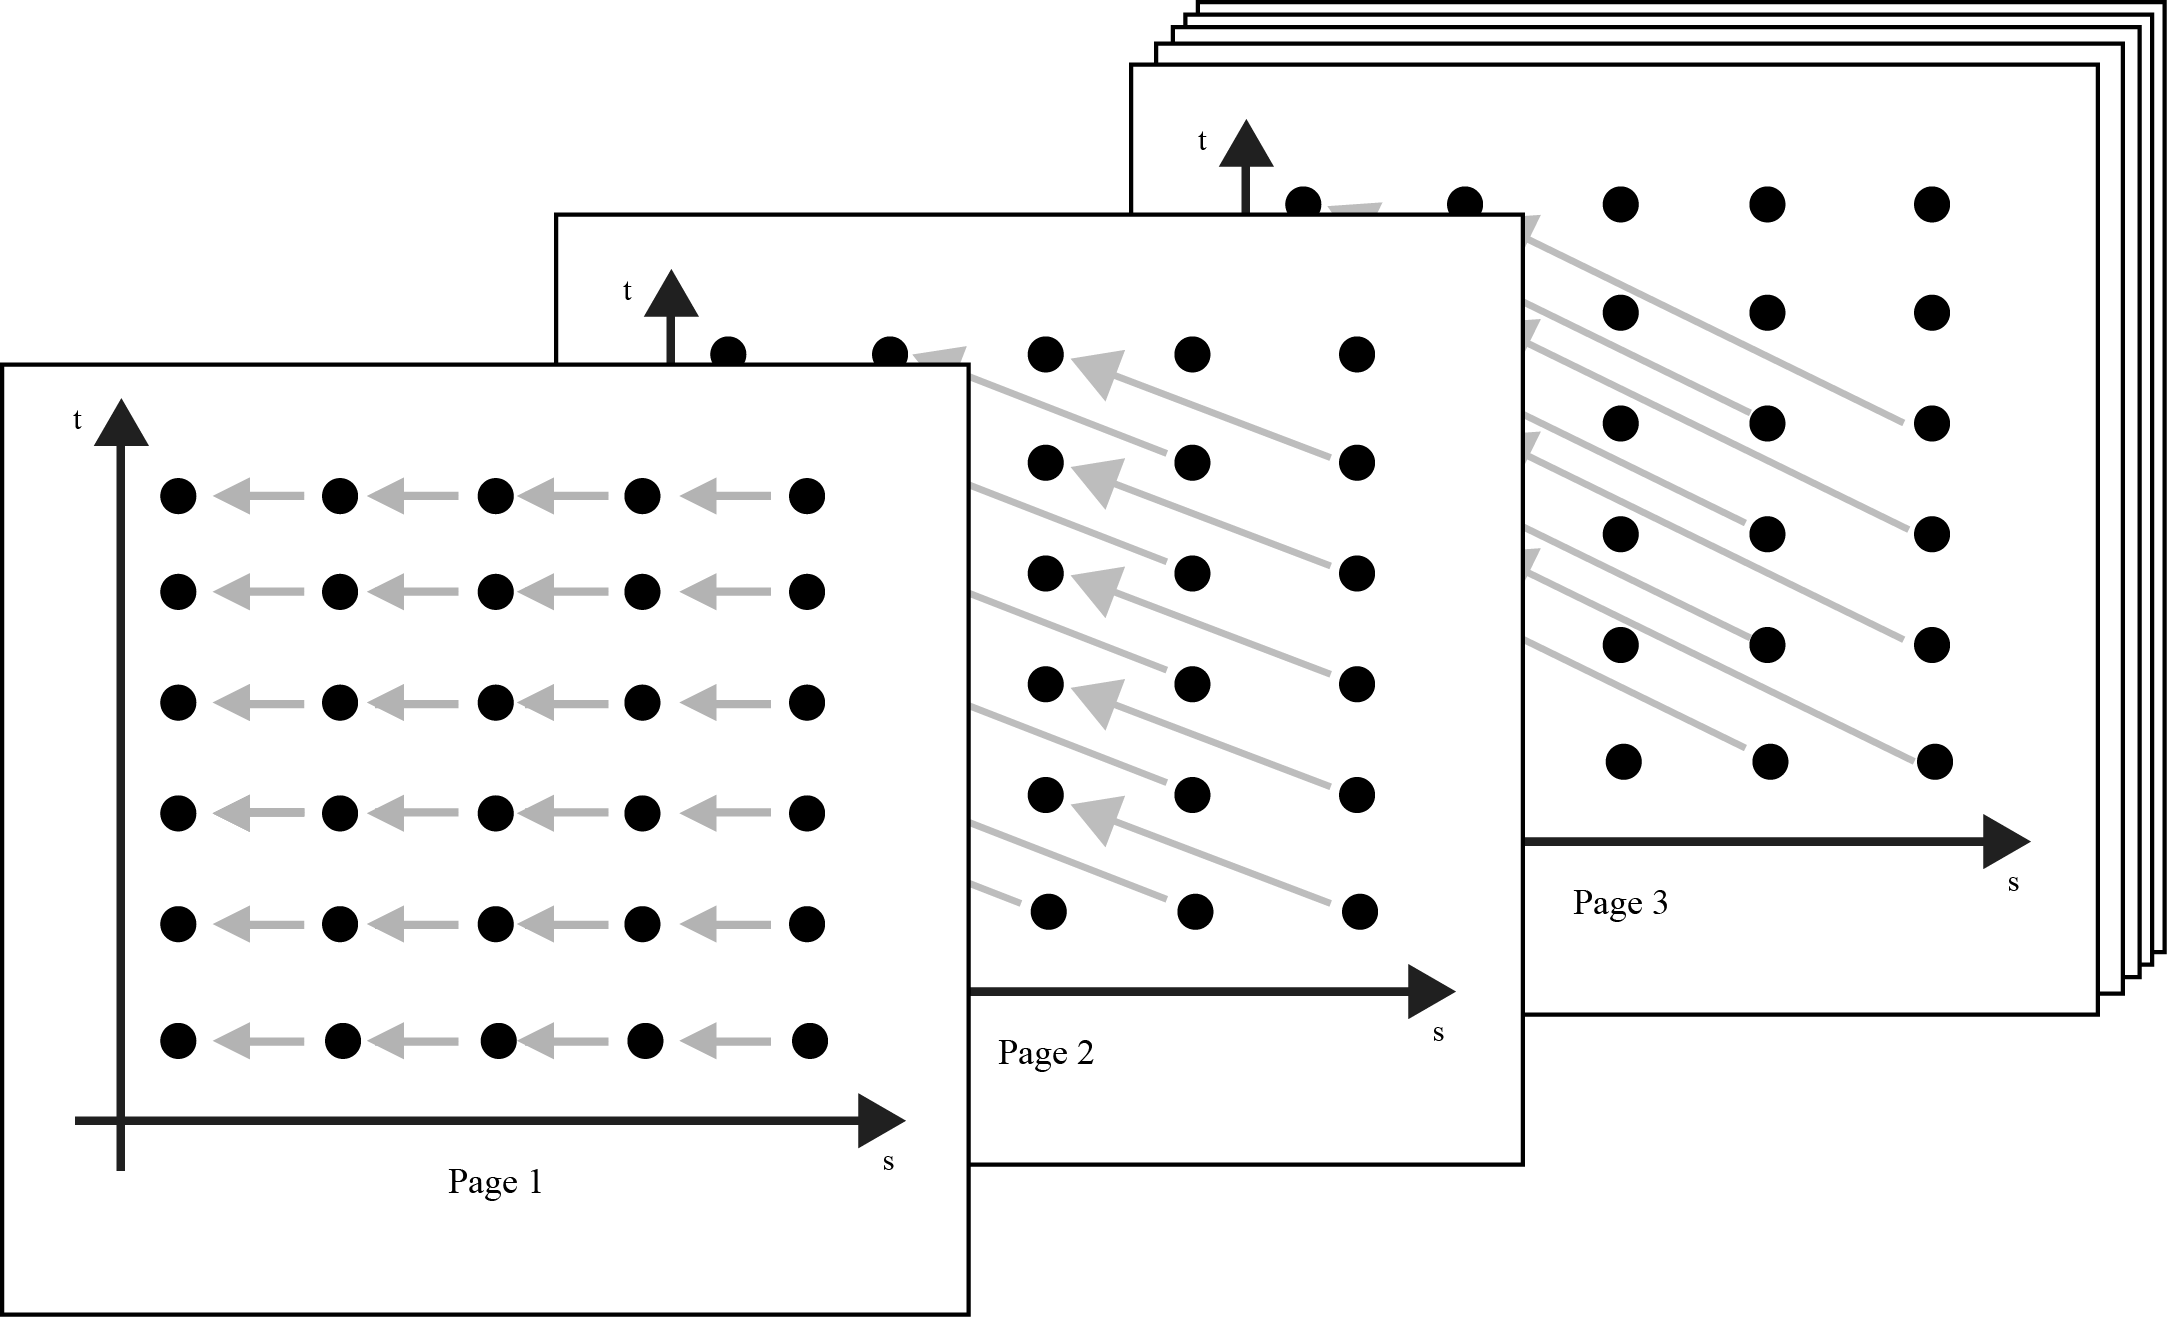
\includegraphics[width=\linewidth,height=0.45\textheight,keepaspectratio]{figures/cover.png}
  \end{center}
       \begin{minipage}{.35\linewidth}
    \begin{flushleft}
      \vspace{2em}
      {\fontsize{6pt}{2pt} \textit{Notes: These are notes live-tex'd
from a graduate course in 4-Manifolds taught by Philip Engel at the
University of Georgia in Spring 2021. As such, any errors or
inaccuracies are almost certainly my own. } } \\
    \end{flushleft}
    \end{minipage}
    \hfill
    \begin{minipage}{.65\linewidth}
    \end{minipage}
  }







\begin{document}

\date{}
\author{D. Zack Garza}
\maketitle
\begin{flushleft}
\textit{D. Zack Garza} \\
\textit{University of Georgia} \\
  \textit{\href{mailto: dzackgarza@gmail.com}{dzackgarza@gmail.com}} \\
{\tiny \textit{Last updated:} 2021-05-11 }
\end{flushleft}


\newpage

% Note: addsec only in KomaScript
\addsec{Table of Contents}
\tableofcontents
\newpage

\hypertarget{tuesday-january-12}{%
\section{Tuesday, January 12}\label{tuesday-january-12}}

\hypertarget{background}{%
\subsection{Background}\label{background}}

From Phil's email:

There are very few references in the notes, and I'll try to update them
to include more as we go. Personally, I found the following online
references particularly useful:

\begin{itemize}
\item
  Dietmar Salamon: Spin Geometry and Seiberg-Witten Invariants
  \autocite{Dietmar99}
\item
  Richard Mandelbaum: Four-dimensional Topology: An Introduction
  \autocite{Mandelbaum1980}

  \begin{itemize}
  \tightlist
  \item
    This book has a nice introduction to surgery aspects of
    four-manifolds, but as a warning: It was published right before
    Freedman's famous theorem. For instance, the existence of an exotic
    R\^{}4 was not known. This actually makes it quite useful, as a
    summary of what was known before, and provides the historical
    context in which Freedman's theorem was proven.
  \end{itemize}
\item
  Danny Calegari: Notes on 4-Manifolds \autocite{Calegari}
\item
  Yuli Rudyak: Piecewise Linear Structures on Topological Manifolds
  \autocite{Rudyak}
\item
  Akhil Mathew: The Dirac Operator \autocite{Matthew}
\item
  Tom Weston: An Introduction to Cobordism Theory \autocite{Weston}

  A wide variety of lecture notes on the Atiyah-Singer index theorem,
  which are available online.
\end{itemize}

\hypertarget{introduction}{%
\subsection{Introduction}\label{introduction}}

\begin{definition}[Topological Manifold]

Recall that a \textbf{topological manifold} (or \(C^0\) manifold) \(X\)
is a Hausdorff topological space \emph{locally homeomorphic} to
\({\mathbb{R}}^n\) with a countable topological base, so we have charts
\(\phi_u: U\to {\mathbb{R}}^n\) which are homeomorphisms from open sets
covering \(X\).

\end{definition}

\begin{example}[The circle]

\(S^1\) is covered by two charts homeomorphic to intervals:

\begin{figure}
\centering
\resizebox{\columnwidth}{!}{%
\begin{tikzpicture}
\node (node_one) at (0,0) { \fontsize{45pt}{1em} \import{/home/zack/SparkleShare/github.com/Notes/Class_Notes/2021/Spring/FourManifolds/sections/figures/}{2021-01-16_21-54.pdf_tex} };
\end{tikzpicture}
}
\end{figure}

\end{example}

\begin{remark}

Maps that are merely continuous are poorly behaved, so we may want to
impose extra structure. This can be done by imposing restrictions on the
transition functions, defined as
\begin{align*}
t_{uv} \coloneqq\varphi_V \to \varphi_U ^{-1} : \varphi_U(U \cap V) \to \varphi_V(U \cap V)
.\end{align*}

\end{remark}

\begin{definition}[Restricted Structures on Manifolds]

\envlist

\begin{itemize}
\item
  We say \(X\) is a \textbf{PL manifold} if and only if \(t_{UV}\) are
  piecewise-linear. Note that an invertible PL map has a PL inverse.
\item
  We say \(X\) is a \textbf{\(C^k\) manifold} if they are \(k\) times
  continuously differentiable, and \textbf{smooth} if infinitely
  differentiable.
\item
  We say \(X\) is \textbf{real-analytic} if they are locally given by
  convergent power series.
\item
  We say \(X\) is \textbf{complex-analytic} if under the identification
  \({\mathbb{R}}^n \cong {\mathbb{C}}^{n/2}\) if they are holomorphic,
  i.e.~the differential of \(t_{UV}\) is complex linear.
\item
  We say \(X\) is a \textbf{projective variety} if it is the vanishing
  locus of homogeneous polynomials on \({\mathbb{CP}}^N\).
\end{itemize}

\end{definition}

\begin{remark}

Is this a strictly increasing hierarchy? It's not clear e.g.~that every
\(C^k\) manifold is PL.

\end{remark}

\begin{question}

Consider \({\mathbb{R}}^n\) as a topological manifold: are any two
smooth structures on \({\mathbb{R}}^n\) diffeomorphic?

\end{question}

\begin{remark}

Fix a copy of \({\mathbb{R}}\) and form a single chart
\({\mathbb{R}}\xrightarrow{\operatorname{id}} {\mathbb{R}}\). There is
only a single transition function, the identity, which is smooth. But
consider
\begin{align*}
X &\to {\mathbb{R}}\\
t &\mapsto t^3
.\end{align*}
This is also a smooth structure on \(X\), since the transition function
is the identity. This yields a different smooth structure, since these
two charts don't like in the same maximal atlas. Otherwise there would
be a transition function of the form \(t_{VU}: t\mapsto t^{1/3}\), which
is not smooth at zero. However, the map
\begin{align*}
X &\to X \\
t &\mapsto t^3
.\end{align*}
defines a diffeomorphism between the two smooth structures.

\end{remark}

\begin{claim}

\({\mathbb{R}}\) admits a unique smooth structure.

\end{claim}

\begin{proof}[sketch]

Let \(\tilde {\mathbb{R}}\) be some exotic \({\mathbb{R}}\), i.e.~a
smooth manifold homeomorphic to \({\mathbb{R}}\). Cover this by
coordinate charts to the standard \({\mathbb{R}}\):

\begin{figure}
\centering
\resizebox{\columnwidth}{!}{%
\begin{tikzpicture}
\node (node_one) at (0,0) { \import{/home/zack/SparkleShare/github.com/Notes/Class_Notes/2021/Spring/FourManifolds/sections/figures}{2021-01-16_22-31.pdf_tex} };
\end{tikzpicture}
}
\end{figure}

\begin{fact}

There exists a cover which is \emph{locally finite} and supports a
\emph{partition of unity}: a collection of smooth functions
\(f_i: U_i \to {\mathbb{R}}\) with \(f_i \geq 0\) and
\({\operatorname{supp}}f \subseteq U_i\) such that \(\sum f_i = 1\)
(\emph{i.e., bump functions}). It is also a purely topological fact that
\(\tilde {\mathbb{R}}\) is orientable.

\end{fact}

So we have bump functions:

\begin{figure}
\centering
\resizebox{\columnwidth}{!}{%
\begin{tikzpicture}
\node (node_one) at (0,0) { \import{/home/zack/SparkleShare/github.com/Notes/Class_Notes/2021/Spring/FourManifolds/sections/figures}{2021-01-16_22-37.pdf_tex} };
\end{tikzpicture}
}
\end{figure}

Take a smooth vector field \(V_i\) on \(U_i\) everywhere aligning with
the orientation. Then \(\sum f_i V_i\) is a smooth nowhere vector field
on \(X\) that is nowhere zero in the direction of the orientation.
Taking the associated flow
\begin{align*}
{\mathbb{R}}&\to \tilde {\mathbb{R}}\\
t &\mapsto \varphi(t)
.\end{align*}
such that \(\varphi'(t) = V(\varphi(t))\). Then \(\varphi\) is a smooth
map that defines a diffeomorphism. This follows from the fact that the
vector field is everywhere positive.

\begin{slogan}

To understand smooth structures on \(X\), we should try to solve
differential equations on \(X\).

\end{slogan}

\end{proof}

\begin{remark}

Note that here we used the existence of a global frame, i.e.~a
trivialization of the tangent bundle, so this doesn't quite work for
e.g.~\(S^2\).

\end{remark}

\begin{question}

What is the difference between all of the above structures? Are there
obstructions to admitting any particular one?

\end{question}

\begin{answer}

\envlist

\begin{enumerate}
\def\labelenumi{\arabic{enumi}.}
\item
  (Munkres) Every \(C^1\) structure gives a unique \(C^k\) and
  \(C^ \infty\) structure.\footnote{Note that this doesn't start at
    \(C^0\), so topological manifolds are genuinely different! There
    exist topological manifolds with no smooth structure.}
\item
  (Grauert) Every \(C^ \infty\) structure gives a unique real-analytic
  structure.
\item
  Every PL manifold admits a smooth structure in \(\dim X \leq 7\), and
  it's unique in \(\dim X\leq 6\), and above these dimensions there
  exists PL manifolds with no smooth structure.
\item
  (Kirby--Siebenmann) Let \(X\) be a topological manifold of
  \(\dim X\geq 5\), then there exists a cohomology class
  \(\operatorname{ks}(X) \in H^4(X; {\mathbb{Z}}/2{\mathbb{Z}})\) which
  is 0 if and only if \(X\) admits a PL structure. Moreover, if
  \(\operatorname{ks}(X) = 0\), then (up to concordance) the set of PL
  structures is given by \(H^3(X; {\mathbb{Z}}/2{\mathbb{Z}})\).
\item
  (Moise) Every topological manifold in \(\dim X\leq 3\) admits a unique
  smooth structure.
\item
  (Smale et al.): In \(\dim X\geq 5\), the number of smooth structures
  on a topological manifold \(X\) is finite. In particular,
  \({\mathbb{R}}^n\) for \(n \neq 4\) has a unique smooth structure. So
  dimension 4 is interesting!
\item
  (Taubes) \({\mathbb{R}}^4\) admits uncountably many non-diffeomorphic
  smooth structures.
\item
  A compact oriented smooth surface \(\Sigma\), the space of
  complex-analytic structures is a complex orbifold \footnote{Locally
    admits a chart to \({\mathbb{C}}^n/ \Gamma\) for \(\Gamma\) a finite
    group.} of dimension \(3g-2\) where \(g\) is the genus of
  \(\Sigma\), up to biholomorphism (i.e.~\emph{moduli}).
\end{enumerate}

\end{answer}

\begin{remark}

Kervaire-Milnor: \(S^7\) admits 28 smooth structures, which form a
group.

\end{remark}

\hypertarget{friday-january-15}{%
\section{Friday, January 15}\label{friday-january-15}}

\begin{remark}

Let
\begin{align*}
V &\coloneqq\left\{{a^2 + b^2 + c^2 + d^3 + e^{6k-1} = 0}\right\} \subseteq {\mathbb{C}}^5 \\
S_\varepsilon&\coloneqq\left\{{ {\left\lvert {a} \right\rvert}^2 + {\left\lvert {b} \right\rvert}^2 + {\left\lvert {c} \right\rvert}^2 + {\left\lvert {d} \right\rvert}^2 + {\left\lvert {e} \right\rvert}^2}\right\}
.\end{align*}
Then \(V_k \cap S_\varepsilon\cong S^7\) is a homeomorphism, and taking
\(k=1,2,\cdots, 28\) yields the 28 smooth structures on \(S^7\). Note
that \(V_k\) is the cone over \(V_k \cap S_\varepsilon\).

\begin{figure}
\centering
\resizebox{\columnwidth}{!}{%
\begin{tikzpicture}
\node (node_one) at (0,0) { 
\fontsize{25pt}{1em} 
\import{/home/zack/SparkleShare/github.com/Notes/Class_Notes/2021/Spring/FourManifolds/sections/figures/}{2021-01-15_13-54.pdf_tex} };
\end{tikzpicture}
}
\end{figure}

\begin{quote}
? Admits a smooth structure, and
\(\mkern 1.5mu\overline{\mkern-1.5muV\mkern-1.5mu}\mkern 1.5mu_k \subseteq {\mathbb{CP}}^5\)
admits no smooth structure.
\end{quote}

\end{remark}

\begin{question}

Is every triangulable manifold PL, i.e.~homeomorphic to a simplicial
complex?

\end{question}

\begin{answer}

No! Given a simplicial complex, there is a notion of the
\textbf{combinatorial link} \(L_V\) of a vertex \(V\):

\begin{figure}
\centering
\resizebox{\columnwidth}{!}{%
\begin{tikzpicture}
\node (node_one) at (0,0) {
\import{/home/zack/SparkleShare/github.com/Notes/Class_Notes/2021/Spring/FourManifolds/sections/figures/}{2021-01-15_13-57.pdf_tex} };
\end{tikzpicture}
}
\end{figure}

It turns out that there exist simplicial manifolds such that the link is
not homeomorphic to a sphere, whereas every PL manifold admits a ``PL
triangulation'' where the links are spheres.

\end{answer}

\begin{remark}

What's special in dimension 4? Recall the \textbf{Kirby-Siebenmann}
invariant \(\operatorname{ks}(x) \in H^4(X; {\mathbb{Z}}_2)\) for \(X\)
a topological manifold where \(\operatorname{ks}(X) = 0 \iff X\) admits
a PL structure, with the caveat that \(\dim X \geq 5\). We can use this
to cook up an invariant of 4-manifolds.

\end{remark}

\begin{definition}[Kirby-Siebenmann Invariant of a 4-manifold]

Let \(X\) be a topological 4-manifold, then
\begin{align*}
\operatorname{ks}(X) \coloneqq\operatorname{ks}(X \times{\mathbb{R}})
.\end{align*}

\end{definition}

\begin{remark}

Recall that in \(\dim X\geq 7\), every PL manifold admits a smooth
structure, and we can note that
\begin{align*}
H^4(X; {\mathbb{Z}}_2) = H^4(X \times{\mathbb{R}}; {\mathbb{Z}}_2) = {\mathbb{Z}}_2,
.\end{align*}
since every oriented 4-manifold admits a fundamental class. Thus
\begin{align*}
\operatorname{ks}(X) = 
\begin{cases}
0 & X \times{\mathbb{R}}\text{ admits a PL and smooth structure} 
\\
1 & X \times{\mathbb{R}}\text{ admits no PL or smooth structures }.
\end{cases}
\end{align*}

\end{remark}

\begin{remark}

\(\operatorname{ks}(X) \neq 0\) implies that \(X\) has no smooth
structure, since \(X \times{\mathbb{R}}\) doesn't. Note that it was not
known if this invariant was nonzero for a while!

\end{remark}

\begin{remark}

Note that \(H^2(X; {\mathbb{Z}})\) admits a symmetric bilinear form
\(Q_X\) defined by
\begin{align*}
{\left\langle { \alpha},~{ \beta} \right\rangle} \mapsto \int_X \alpha\wedge \beta = \alpha \smile\beta([X]) \in {\mathbb{Z}}
.\end{align*}
where \([X]\) is the fundamental class.

\end{remark}

\hypertarget{main-theorems-for-the-course}{%
\section{Main Theorems for the
Course}\label{main-theorems-for-the-course}}

Proving the following theorems is the main goal of this course.

\begin{theorem}[Freedman]

If \(X, Y\) are compact oriented topological 4-manifolds, then
\(X\cong Y\) are homeomorphic if and only if
\(\operatorname{ks}(X) = \operatorname{ks}(Y)\) and \(Q_X \cong Q_Y\)
are isometric, i.e.~there exists an isometry
\begin{align*}
\varphi: H^2(X; {\mathbb{Z}}) \to H^2(Y; {\mathbb{Z}})
.\end{align*}
that preserves the two bilinear forms in the sense that
\({\left\langle {\varphi \alpha},~{ \varphi \beta} \right\rangle} = {\left\langle { \alpha},~{ \beta} \right\rangle}\).

Conversely, every \textbf{unimodular} bilinear form appears as
\(H^2(X; {\mathbb{Z}})\) for some \(X\), i.e.~the pairing induces a map
\begin{align*}
H^2(X; {\mathbb{Z}}) &\to H^2(X; {\mathbb{Z}})^\vee\\
\alpha \mapsto {\left\langle { \alpha },~{ {-}} \right\rangle}
.\end{align*}
which is an isomorphism. This is essentially a classification of
simply-connected 4-manifolds.

\end{theorem}

\begin{remark}

Note that preservation of a bilinear form is a stand-in for ``being an
element of the orthogonal group'', where we only have a lattice instead
of a full vector space.

\end{remark}

\begin{remark}

There is a map
\(H^2(X; {\mathbb{Z}}) \xrightarrow{PD} H_2(X; {\mathbb{Z}})\) from
Poincaré , where we can think of elements in the latter as closed
surfaces \([\Sigma]\), and
\begin{align*}
{\left\langle { \Sigma_1 },~{ \Sigma_2 } \right\rangle} = \text{signed number of intersections points of } \Sigma_1 \pitchfork\Sigma_2
.\end{align*}
Note that Freedman's theorem is only about homeomorphism, and is not
true smoothly. This gives a way to show that two 4-manifolds are
homeomorphic, but this is hard to prove! So we'll black-box this, and
focus on ways to show that two \emph{smooth} 4-manifolds are \emph{not}
diffeomorphic, since we want homeomorphic but non-diffeomorphic
manifolds.

\end{remark}

\begin{definition}[Signature]

The \textbf{signature} of a topological 4- manifold is the signature of
\(Q_X\), where we note that \(Q_X\) is a symmetric nondegenerate
bilinear form on \(H^2(X; {\mathbb{R}})\) and for some \(a, b\)
\begin{align*}
(H^2(X; {\mathbb{R}}), Q_x) \xrightarrow{\text{isometric}} {\mathbb{R}}^{a, b}
.\end{align*}
where \(a\) is the number of \(+1\)s appearing in the matrix and \(b\)
is the number of \(-1\)s. This is \({\mathbb{R}}^{ab}\) where
\(e_i^2 = 1, i=1\cdots a\) and \(e_i^2 = -1, i=a+1, \cdots b\), and is
thus equipped with a specific bilinear form corresponding to the Gram
matrix of this basis.
\begin{align*}
\begin{bmatrix}
1 & 0 & 0 & 0 & 0
\\
0 & 1 & 0 & 0 & 0
\\
0 & 0 & \ddots & 0 & 0
\\
0 & 0 & 0 & -1 & 0
\\
0 & 0 & 0 & 0 & -1
\end{bmatrix}
= I_{a\times a} \oplus -I_{b \times b}
.\end{align*}
Then the signature is \(a-b\), the dimension of the positive-definite
space minus the dimension of the negative-definite space.

\end{definition}

\begin{theorem}[Rokhlin's Theorem]

Suppose
\({\left\langle { \alpha},~{\alpha} \right\rangle} \in 2{\mathbb{Z}}\)
and \(\alpha\in H^2(X; {\mathbb{Z}})\) and \(X\) a simply connected
\textbf{smooth} 4-manifold. Then 16 divides \(\operatorname{sig}(X)\).

\end{theorem}

\begin{remark}

Note that Freedman's theorem implies that there exists topological
4-manifolds with no smooth structure.

\end{remark}

\begin{theorem}[Donaldson]

Let \(X\) be a smooth simply-connected 4-manifold. If \(a=0\) or
\(b=0\), then \(Q_X\) is diagonalizable and there exists an orthonormal
basis of \(H^2(X; {\mathbb{Z}})\).

\end{theorem}

\begin{remark}

This comes from Gram-Schmidt, and restricts what types of intersection
forms can occur.

\end{remark}

\hypertarget{warm-up-mathbbr2-has-a-unique-smooth-structure}{%
\subsection{\texorpdfstring{Warm Up: \({\mathbb{R}}^2\) Has a Unique
Smooth
Structure}{Warm Up: \{\textbackslash mathbb\{R\}\}\^{}2 Has a Unique Smooth Structure}}\label{warm-up-mathbbr2-has-a-unique-smooth-structure}}

\begin{remark}

Last time we showed \({\mathbb{R}}^1\) had a unique smooth structure, so
now we'll do this for \({\mathbb{R}}^2\). The strategy of solving a
differential equation, we'll now sketch the proof.

\end{remark}

\begin{definition}[Riemannian Metrics]

A \textbf{Riemannian metric} \(g\in \operatorname{Sym}^2 T^*X\) for
\(X\) a smooth manifold is a metric on every \(T_p X\) given by
\begin{align*}
g_p: T_pX \times T_p X &\to {\mathbb{R}}\\
g(v, v) \geq 0, g(v,v) = 0 \iff v=0
.\end{align*}

\end{definition}

\begin{definition}[Almost complex structure]

An \textbf{almost complex structure} is a
\(J\in \mathop{\mathrm{End}}(TX)\) such that
\(J^2 = -\operatorname{id}\).

\end{definition}

\begin{remark}

Let \(e\in T_p X\) and \(e\neq 0\), then if \(X\) is a surface then
\(\left\{{e, Je}\right\}\) is a basis of \(T_p X\).

\begin{figure}
\centering
\resizebox{\columnwidth}{!}{%
\begin{tikzpicture}
\node (node_one) at (0,0) { 
\fontsize{25pt}{1em} 
\import{/home/zack/SparkleShare/github.com/Notes/Class_Notes/2021/Spring/FourManifolds/sections/figures/}{2021-01-15_14-33.pdf_tex} };
\end{tikzpicture}
}
\end{figure}

This is a basis because if \(Je\) and \(e\) are parallel, then ??? In
particular, \(J_p\) is determined by a point in
\({\mathbb{R}}^2\setminus\left\{{\text{the }x{\hbox{-}}\text{axis}}\right\}\)

\end{remark}

\hypertarget{sketch-of-proof}{%
\subsubsection{Sketch of Proof}\label{sketch-of-proof}}

Let \(\tilde {\mathbb{R}}^2\) be an exotic \({\mathbb{R}}^2\).

\hypertarget{step-1}{%
\paragraph{Step 1}\label{step-1}}

Choose a metric on \(\tilde {\mathbb{R}}^2\) \(g \coloneqq\sum f_I g_i\)
with \(g_i\) metrics on coordinate charts \(U_i\) and \(f_i\) a
partition of unity.

\hypertarget{step-2}{%
\paragraph{Step 2}\label{step-2}}

Find an almost complex structure on \(\tilde {\mathbb{R}}^2\). Choosing
an orientation of \(\tilde {\mathbb{R}}^2\), \(g\) defines a unique
almost complex structure
\(J_p e \coloneqq f\in T_p \tilde {\mathbb{R}}^2\) such that

\begin{itemize}
\tightlist
\item
  \(g(e, e) = g(f, f)\)
\item
  \(g(e, f) = 0\).
\item
  \(\left\{{e, f}\right\}\) is an oriented basis of
  \(T_p \tilde {\mathbb{R}}^2\)
\end{itemize}

This is because after choosing \(e\), there are two orthogonal vectors,
but only one choice yields an \emph{oriented} basis.

\begin{figure}
\centering
\resizebox{\columnwidth}{!}{%
\begin{tikzpicture}
\node (node_one) at (0,0) {
\fontsize{25pt}{1em} 
  \import{/home/zack/SparkleShare/github.com/Notes/Class_Notes/2021/Spring/FourManifolds/sections/figures/}{2021-01-15_14-39.pdf_tex}
  };
\end{tikzpicture}
}
\end{figure}

\hypertarget{step-3}{%
\paragraph{Step 3}\label{step-3}}

We then apply a theorem:

\begin{theorem}[?]

Any almost complex structure on a surface comes from a complex
structure, in the sense that there exist charts
\(\varphi_i: U_i \to {\mathbb{C}}\) such that \(J\) is multiplication by
\(i\).

\end{theorem}

So \(d \varphi(J \cdot e) = i \cdot d \varphi_i (e)\), and
\((\tilde {\mathbb{R}}^2, J)\) is a complex manifold. Since it's simply
connected, the Riemann Mapping Theorem shows that it's biholomorphic to
\({\mathbb{D}}\) or \({\mathbb{C}}\), both of which are diffeomorphic to
\({\mathbb{R}}^2\).

\begin{quote}
See the Newlander-Nirenberg theorem, a result in complex geometry.
\end{quote}

\hypertarget{lecture-3-wednesday-january-20}{%
\section{Lecture 3 (Wednesday, January
20)}\label{lecture-3-wednesday-january-20}}

Today: some background material on sheaves, bundles, connections.

\hypertarget{sheaves}{%
\subsection{Sheaves}\label{sheaves}}

\begin{definition}[Presheaves and Sheaves]

Recall that if \(X\) is a topological space, a \textbf{presheaf} of
abelian groups \(\mathcal{F}\) is an assignment \(U\to \mathcal{F}(U)\)
of an abelian group to every open set \(U \subseteq X\) together with a
restriction map \(\rho_{UV}: \mathcal{F}(U) \to \mathcal{F}(V)\) for any
inclusion \(V \subseteq U\) of open sets. This data has to satisfying
certain conditions:

\begin{enumerate}
\def\labelenumi{\alph{enumi}.}
\item
  \(\mathcal{F}(\emptyset) = 0\), the trivial abelian group.
\item
  \(\rho_{UU}: \mathcal{F}(U) \to \mathcal{F}(U) = \operatorname{id}_{\mathcal{F}(U) }\)
\item
  Compatibility if restriction is taken in steps:
  \(U \subseteq V \subseteq W \implies \rho_{VW} \circ \rho_{UV} = \rho_{UW}\).
\end{enumerate}

We say \(\mathcal{F}\) is a \textbf{sheaf} if additionally:

\begin{enumerate}
\def\labelenumi{\alph{enumi}.}
\setcounter{enumi}{3}
\tightlist
\item
  Given \(s_i \in \mathcal{F}(U_i)\) such that
  \(\rho_{U_i \cap U_j} (s_i) = \rho_{U_i \cap U_j} (s_j)\) implies that
  there exists a unique \(s\in \mathcal{F}(\bigcup_i U_i)\) such that
  \(\rho_{U_i}(s) = s_i\).
\end{enumerate}

\begin{figure}
\centering
\resizebox{\columnwidth}{!}{%
\begin{tikzpicture}
\node (node_one) at (0,0) { 
\fontsize{45pt}{1em} 
\import{/home/zack/SparkleShare/github.com/Notes/Class_Notes/2021/Spring/FourManifolds/sections/figures}{2021-01-20_13-59.pdf_tex} };
\end{tikzpicture}
}
\end{figure}

\end{definition}

\begin{example}[?]

Let \(X\) be a topological manifold, then
\(\mathcal{F}\coloneqq C^0({-}, {\mathbb{R}})\) the set of continuous
functionals form a sheaf. We have a diagram

\begin{center}
\begin{tikzcd}
    U && {C^0(U; {\mathbb{R}})} \\
    \\
    V && {C^0(V; {\mathbb{R}})}
    \arrow[hook, from=3-1, to=1-1]
    \arrow["{\text{restrict cts. functions}}", dashed, hook, from=1-3, to=3-3]
    \arrow["{\mathcal{F}}", from=1-1, to=1-3]
    \arrow["{\mathcal{F}}"', from=3-1, to=3-3]
\end{tikzcd}
\end{center}

\begin{quote}
\href{https://q.uiver.app/?q=WzAsNCxbMCwwLCJVIl0sWzAsMiwiViJdLFsyLDAsIkNeMChVOyBcXFJSKSJdLFsyLDIsIkNeMChWOyBcXFJSKSJdLFsxLDAsIiIsMCx7InN0eWxlIjp7InRhaWwiOnsibmFtZSI6Imhvb2siLCJzaWRlIjoidG9wIn19fV0sWzIsMywiXFx0ZXh0e3Jlc3RyaWN0IGN0cy4gZnVuY3Rpb25zfSIsMCx7InN0eWxlIjp7InRhaWwiOnsibmFtZSI6Imhvb2siLCJzaWRlIjoidG9wIn0sImJvZHkiOnsibmFtZSI6ImRhc2hlZCJ9fX1dLFswLDIsIlxcbWF0aGNhbHtGfSJdLFsxLDMsIlxcbWF0aGNhbHtGfSIsMl1d}{Link
to diagram}
\end{quote}

Property (d) holds because given sections
\(s_i \in C^0(U_i; {\mathbb{R}})\) agreeing on overlaps, so
\({ \left.{{s_i}} \right|_{{U_i \cap U_j}} } = { \left.{{s_j}} \right|_{{U_i \cap U_j}} }\),
there exists a unique \(s\in C^0(\bigcup_i U_i; {\mathbb{R}})\) such
that \({ \left.{{s}} \right|_{{U_i}} } = s_i\) for all \(i\) --
continuous functions glue.

\end{example}

\begin{remark}

Recall that we discussed various structures on manifolds: PL,
continuous, smooth, complex-analytic, etc. We can characterize these by
their sheaves of functions, which we'll denote \({\mathcal{O}}\). For
example, \({\mathcal{O}}\coloneqq C^0({-}; {\mathbb{R}})\) for
topological manifolds, and
\({\mathcal{O}}\coloneqq C^ \infty ({-}; {\mathbb{R}})\) is the sheaf
for smooth manifolds. Note that this also works for PL functions, since
pullbacks of PL functions are again PL. For complex manifolds, we set
\({\mathcal{O}}\) to be the sheaf of holomorphic functions.

\end{remark}

\begin{example}[Locally Constant Sheaves]

Let \(A\in {\mathsf{Ab}}\) be an abelian group, then \(\underline{A}\)
is the sheaf defined by setting \(\underline{A}(U)\) to be the locally
constant functions \(U\to A\). E.g. let
\(X \in {\mathsf{Mfd}}_{{\mathsf{Top}}}\) be a topological manifold,
then \(\underline{{\mathbb{R}}}(U) = {\mathbb{R}}\) if \(U\) is
connected since locally constant \(\implies\) globally constant in this
case.

\end{example}

\begin{warnings}

Note that the presheaf of constant functions doesn't satisfy (d)! Take
\({\mathbb{R}}\) and a function with two different values on disjoint
intervals:

\begin{figure}
\centering
\resizebox{\columnwidth}{!}{%
\begin{tikzpicture}
\node (node_one) at (0,0) { 
\fontsize{41pt}{1em} 
\import{/home/zack/SparkleShare/github.com/Notes/Class_Notes/2021/Spring/FourManifolds/sections/figures}{2021-01-20_14-11.pdf_tex} };
\end{tikzpicture}
}
\end{figure}

Note that
\({ \left.{{s_1}} \right|_{{U_1 \cap U_2}} } = { \left.{{s_2}} \right|_{{U_1 \cap U_2}} }\)
since the intersection is empty, but there is no constant function that
restricts to the two different values.

\end{warnings}

\hypertarget{bundles}{%
\subsection{Bundles}\label{bundles}}

\begin{remark}

Let \(\pi: \mathcal{E}\to X\) be a \textbf{vector bundle}, so we have
local trivializations \(\pi ^{-1} (U) \xrightarrow{h_u} Y^d \times U\)
where we take either \(Y={\mathbb{R}}, {\mathbb{C}}\), such that
\(h_v \circ h_u ^{-1}\) preserves the fibers of \(\pi\) and acts
linearly on each fiber of \(Y\times(U \cap V)\). Define
\begin{align*}
t_{UV}: U \cap V \to \operatorname{GL}_d(Y)
\end{align*}
where we require that \(t_{UV}\) is continuous, smooth,
complex-analytic, etc depending on the context.

\begin{figure}
\centering
\resizebox{\columnwidth}{!}{%
\begin{tikzpicture}
\node (node_one) at (0,0) { 
\fontsize{47pt}{1em} 
\import{/home/zack/SparkleShare/github.com/Notes/Class_Notes/2021/Spring/FourManifolds/sections/figures}{2021-01-20_14-17.pdf_tex} };
\end{tikzpicture}
}
\end{figure}

\end{remark}

\begin{example}[Bundles over $S^1$]

There are two \({\mathbb{R}}^1\) bundles over \(S^1\):

\begin{figure}
\centering
\resizebox{\columnwidth}{!}{%
\begin{tikzpicture}
\node (node_one) at (0,0) { 
\fontsize{32pt}{1em} 
\import{/home/zack/SparkleShare/github.com/Notes/Class_Notes/2021/Spring/FourManifolds/sections/figures}{2021-01-20_14-20.pdf_tex} };
\end{tikzpicture}
}
\end{figure}

Note that the Mobius bundle is not trivial, but can be locally
trivialized.

\end{example}

\begin{remark}

We abuse notation: \(\mathcal{E}\) is also a sheaf, and we write
\(\mathcal{E}(U)\) to be the set of sections \(s: U\to \mathcal{E}\)
where \(s\) is continuous, smooth, holomorphic, etc where
\(\pi \circ s = \operatorname{id}_U\). I.e. a bundle is a sheaf in the
sense that its sections \emph{form} a sheaf.

\end{remark}

\begin{example}[?]

The trivial line bundle gives the sheaf \({\mathcal{O}}\) : maps
\(U \xrightarrow{s} U\times Y\) for \(Y={\mathbb{R}}, {\mathbb{C}}\)
such that \(\pi \circ s = \operatorname{id}\) are the same as maps
\(U\to Y\).

\end{example}

\begin{definition}[$\OO\dash$modules]

An \textbf{\({\mathcal{O}}{\hbox{-}}\)module} is a sheaf \(\mathcal{F}\)
such that \(\mathcal{F}(U)\) has an action of \(\mathcal{O}(U)\)
compatible with restriction.

\end{definition}

\begin{example}[?]

If \(\mathcal{E}\) is a vector bundle, then \(\mathcal{E}(U)\) has a
natural action of \({\mathcal{O}}(U)\) given by
\(f\curvearrowright s \coloneqq fs\), i.e.~just multiplying functions.

\end{example}

\begin{example}[Non-example]

The locally constant sheaf \(\underline{{\mathbb{R}}}\) is not an
\({\mathcal{O}}{\hbox{-}}\)module: there isn't natural action since the
sections of \({\mathcal{O}}\) are generally non-constant functions, and
multiplying a constant function by a non-constant function doesn't
generally give back a constant function.

\end{example}

We'd like a notion of maps between sheaves:

\begin{definition}[Morphisms of Sheaves]

A \textbf{morphism} of sheaves \(\mathcal{F} \to \mathcal{G}\) is a
group morphism \(\varphi(U): \mathcal{F}(U) \to \mathcal{G}(U)\) for all
opens \(U \subseteq X\) such that the diagram involving restrictions
commutes:

\begin{center}
\begin{tikzcd}
\mathcal{F}(U) 
\ar[r, "\phi(U)"] 
\ar[d, "\rho_{UV}"]
&
\mathcal{G}(U) 
\ar[d, "\rho_{UV}"]
\\
\mathcal{F}(V) 
\ar[r, "\phi(V)"] 
&
\mathcal{F}(V) 
\end{tikzcd}
\end{center}

\end{definition}

\begin{example}[An $\OO\dash$module that is not a vector bundle.]

Let \(X = {\mathbb{R}}\) and define the \textbf{skyscraper sheaf} at
\(p \in {\mathbb{R}}\) as
\begin{align*}
{\mathbb{R}}_p(U) \coloneqq
\begin{cases}
{\mathbb{R}}& p\in U 
\\
0 & p\not\in U.
\end{cases}
.\end{align*}

The \({\mathcal{O}}(U){\hbox{-}}\)module structure is given by
\begin{align*}
{\mathcal{O}}(U) \times{\mathcal{O}}(U) &\to {\mathbb{R}}_p(U) \\
(f, s) &\mapsto f(p) s
.\end{align*}
This is not a vector bundle since \({\mathbb{R}}_p(U)\) is not an
infinite dimensional vector space, whereas the space of sections of a
vector bundle is generally infinite dimensional (?). Alternatively,
there are arbitrarily small punctured open neighborhoods of \(p\) for
which the sheaf makes trivial assignments.

\end{example}

\begin{example}[of morphisms]

Let \(X = {\mathbb{R}}\in {\mathsf{Mfd}}_{\operatorname{Sm}}\) viewed as
a smooth manifold, then multiplication by \(x\) induces a morphism of
structure sheaves:
\begin{align*}
(x \cdot): {\mathcal{O}}&\to {\mathcal{O}}\\
s & \mapsto x\cdot s
\end{align*}
for any \(x\in {\mathcal{O}}(U)\), noting that
\(x\cdot s\in {\mathcal{O}}(U)\) again.

\begin{exercise}[?]

Check that \(\ker \varphi\) is naturally a sheaf and
\(\ker(\varphi)(U) = \ker (\varphi(U)): \mathcal{F}(U) \to \mathcal{G}(U)\)

\end{exercise}

Here the kernel is trivial, i.e.~on any open \(U\) we have
\((x\cdot):{\mathcal{O}}(U) \hookrightarrow{\mathcal{O}}(U)\) is
injective. Taking the cokernel \(\operatorname{coker}(x\cdot)\) as a
presheaf, this assigns to \(U\) the quotient presheaf
\({\mathcal{O}}(U) / x{\mathcal{O}}(U)\), which turns out to be equal to
\({\mathbb{R}}_0\). So \({\mathcal{O}}\to {\mathbb{R}}_0\) by
restricting to the value at \(0\), and there is an exact sequence
\begin{align*}
0 \to {\mathcal{O}}\xrightarrow{(x\cdot)} {\mathcal{O}}\to {\mathbb{R}}_0 \to 0
.\end{align*}

This is one reason sheaves are better than vector bundles: the category
is closed under taking quotients, whereas quotients of vector bundles
may not be vector bundles.

\end{example}

\hypertarget{lecture-4-friday-january-22}{%
\section{Lecture 4 (Friday, January
22)}\label{lecture-4-friday-january-22}}

\hypertarget{the-exponential-exact-sequence}{%
\subsection{The Exponential Exact
Sequence}\label{the-exponential-exact-sequence}}

Let \(X = {\mathbb{C}}\) and consider \({\mathcal{O}}\) the sheaf of
holomorphic functions and \({\mathcal{O}}^{\times}\) the sheaf of
\emph{nonvanishing} holomorphic functions. The former is a vector bundle
and the latter is a sheaf of abelian groups. There is a map
\(\exp: {\mathcal{O}}\to {\mathcal{O}}^{\times}\), the
\textbf{exponential map}, which is the data
\(\exp(U): {\mathcal{O}}(U) \to {\mathcal{O}}^{\times}(U)\) on every
open \(U\) given by \(f\mapsto e^f\). There is a kernel sheaf
\(2\pi i \underline{{\mathbb{Z}}}\), and we get an exact sequence
\begin{align*}
0 \to 2\pi i \underline{{\mathbb{Z}}} \to {\mathcal{O}}\xrightarrow{\exp} {\mathcal{O}}^{\times}\to \operatorname{coker}(\exp) \to 0
.\end{align*}

\begin{question}

What is the cokernel sheaf here?

\end{question}

Let \(U\) be a contractible open set, then we can identify
\({\mathcal{O}}^{\times}(U) / \exp({\mathcal{O}}^{\times}(U)) = 1\).

\begin{figure}
\centering
\resizebox{\columnwidth}{!}{%
\begin{tikzpicture}
\node (node_one) at (0,0) { 
\fontsize{44pt}{1em} 
\import{/home/zack/SparkleShare/github.com/Notes/Class_Notes/2021/Spring/FourManifolds/sections/figures}{2021-01-22_13-58.pdf_tex} 
};
\end{tikzpicture}
}
\end{figure}

Any \(f\in {\mathcal{O}}^{\times}(U)\) has a logarithm, say by taking a
branch cut, since \(\pi_1(U) =0 \implies \log f\) has an analytic
continuation. Consider the annulus \(U\) and the function
\(z\in {\mathcal{O}}^{\times}(U)\), then
\(z\not\in \exp({\mathcal{O}}(U))\) -- if \(z=e^f\) then \(f=\log(z)\),
but \(\log(z)\) has monodromy on \(U\):

\begin{figure}
\centering
\resizebox{\columnwidth}{!}{%
\begin{tikzpicture}
\node (node_one) at (0,0) { 
\fontsize{44pt}{1em} 
\import{/home/zack/SparkleShare/github.com/Notes/Class_Notes/2021/Spring/FourManifolds/sections/figures}{2021-01-22_14-02.pdf_tex} 
};
\end{tikzpicture}
}
\end{figure}

Thus on any sufficiently small open set,
\(\operatorname{coker}(\exp) = 1\). This is only a presheaf: there
exists an open cover of the annulus for which
\({ \left.{{z}} \right|_{{U_i}} }\), and so the naive cokernel doesn't
define a sheaf. This is because we have a locally trivial section which
glues to \(z\), which is nontrivial.

\begin{exercise}[?]

Redefine the cokernel so that it is a sheaf. Hint: look at
sheafification, which has the defining property
\(\mathop{\mathrm{Hom}}_{{\mathsf{Presh}}}(\mathcal{G}, \mathcal{F}^{\mathsf{Presh}}) =\mathop{\mathrm{Hom}}_{{\mathsf{Sh}}}( \mathcal{G}, \mathcal{F}^{{\mathsf{Sh}}})\)
for any sheaf \(\mathcal{G}\).

\end{exercise}

\begin{definition}[Global Sections Sheaf]

The \textbf{global sections} sheaf of \(\mathcal{F}\) on \(X\) is given
by \(H^0( X; \mathcal{F}) = \mathcal{F}(X)\).

\end{definition}

\begin{example}[?]

\envlist

\begin{itemize}
\tightlist
\item
  \(C^ \infty (X) = H^0(X, C^ \infty )\) are the smooth functions on
  \(X\)
\item
  \(VF(X) = H^0(X; T)\) are the smooth vector fields on \(X\) for \(T\)
  the tangent bundle
\item
  If \(X\) is a complex manifold then
  \({\mathcal{O}}(X) = H^0(X; {\mathcal{O}})\) are the globally
  holomorphic functions on \(X\).
\item
  \(H^0(X; {\mathbb{Z}}) = \underline{{\mathbb{Z}}}(X)\) are ??
\end{itemize}

\end{example}

\begin{remark}

Given vector bundles \(V, W\), we have constructions
\(V \oplus W, V \otimes W, V^\vee, \mathop{\mathrm{Hom}}(V, W) = V^\vee\otimes W, \operatorname{Sym}^n V, \bigwedge^p V\),
and so on. Some of these work directly for sheaves:

\begin{itemize}
\tightlist
\item
  \(\mathcal{F} \oplus \mathcal{G}(U) \coloneqq\mathcal{F}(U) \oplus \mathcal{G}(U)\)
\item
  For tensors, duals, and homs
  \(\mathscr{H}\kern-2pt\operatorname{om}(V, W)\) we only get
  presheaves, so we need to sheafify.
\end{itemize}

\end{remark}

\begin{warnings}

\(\mathop{\mathrm{Hom}}(V, W)\) will denote the \emph{global}
homomorphisms \(\mathscr{H}\kern-2pt\operatorname{om}(V, W)(X)\), which
is a sheaf.

\end{warnings}

\begin{example}[?]

Let \(X^n \in {\mathsf{Mfd}}_{{\operatorname{sm}}}\) and let
\(\Omega^p\) be the sheaf of smooth \(p{\hbox{-}}\)forms, i.e
\(\bigwedge^p T^\vee\), i.e.~\(\Omega^p(U)\) are the smooth \(p\) forms
on \(U\), which are locally of the form
\(\sum f_{i_1, \cdots, i_p} (x_1, \cdots, x_n) dx_{i_1} \wedge dx_{i_2} \wedge \cdots dx_{i_p}\)
where the \(f_{i_1, \cdots, i_p}\) are smooth functions.

\begin{example}[Sub-example]

Take \(X= S^1\), writing this as \({\mathbb{R}}/{\mathbb{Z}}\), we have
\(\Omega^1(X) \ni dx\). There are two coordinate charts which differ by
a translation on their overlaps, and \(dx(x + c) =dx\) for \(c\) a
constant:

\begin{figure}
\centering
\resizebox{\columnwidth}{!}{%
\begin{tikzpicture}
\node (node_one) at (0,0) { 
\fontsize{44pt}{1em} 
\import{/home/zack/SparkleShare/github.com/Notes/Class_Notes/2021/Spring/FourManifolds/sections/figures}{2021-01-22_14-22.pdf_tex} 
};
\end{tikzpicture}
}
\end{figure}

\end{example}

\begin{exercise}[?]

Check that on a torus, \(dx_i\) is a well-defined 1-form.

\end{exercise}

\end{example}

\begin{remark}

Note that there is a map \(d: \Omega^p \to \Omega^{p+1}\) where
\(\omega\mapsto d \omega\).

\end{remark}

\begin{warnings}

\(d\) is \textbf{not} a map of \({\mathcal{O}}{\hbox{-}}\)modules:
\(d(f\cdot \omega) = f\cdot \omega + {\color{red} df \wedge \omega}\),
where the latter is a correction term. In particular, it is not a map of
vector bundles, but is a map of sheaves of abelian groups since
\(d ( \omega_1 + \omega_2) = d( \omega_1 ) + d ( \omega_2)\), making
\(d\) a sheaf morphism.

\end{warnings}

Let \(X \in {\mathsf{Mfd}}_{\mathbb{C}}\), we'll use the fact that
\(TX\) is complex-linear and thus a \({\mathbb{C}}{\hbox{-}}\)vector
bundle.

\begin{figure}
\centering
\resizebox{\columnwidth}{!}{%
\begin{tikzpicture}
\node (node_one) at (0,0) { 
\fontsize{44pt}{1em} 
\import{/home/zack/SparkleShare/github.com/Notes/Class_Notes/2021/Spring/FourManifolds/sections/figures}{2021-01-22_14-27.pdf_tex} 
};
\end{tikzpicture}
}
\end{figure}

\begin{remark}[Subtlety 1]

Note that \(\Omega^p\) for complex manifolds is \(\bigwedge^p T^\vee\),
and so if we want to view \(X \in {\mathsf{Mfd}}_{\mathbb{R}}\) we'll
write \(X_{{\mathbb{R}}}\). \(TX_{\mathbb{R}}\) is then a real vector
bundle of rank \(2n\).

\end{remark}

\begin{remark}[Subtlety 2]

\(\Omega^p\) will denote \emph{holomorphic} \(p{\hbox{-}}\)forms,
i.e.~local expressions \(\sum f_I(z_1, \cdots, z_n) \bigwedge dz_I\).
For example, \(e^zdz\in \Omega^1({\mathbb{C}})\) but
\(z\mkern 1.5mu\overline{\mkern-1.5muz\mkern-1.5mu}\mkern 1.5mu dz\) is
not, where \(dz = dx + idy\). We'll use a different notation when we
allow the \(f_I\) to just be smooth: \(A^{p, 0}\), the sheaf of
\((p, 0){\hbox{-}}\)forms. Then
\(z\mkern 1.5mu\overline{\mkern-1.5muz\mkern-1.5mu}\mkern 1.5mu dz\in A^{1, 0}\).

\end{remark}

\begin{remark}

Note that
\(T^\vee X_{\mathbb{R}}\otimes _{\mathbb{C}}= A^{1, 0} \oplus A^{0, 1}\)
since there is a unique decomposition
\(\omega = fdz + gd\mkern 1.5mu\overline{\mkern-1.5muz\mkern-1.5mu}\mkern 1.5mu\)
where \(f,g\) are smooth. Then
\(\Omega^d X_{\mathbb{R}}\otimes_{\mathbb{R}}{\mathbb{C}}= \bigoplus _{p+q=d} A^{p, q}\).
Note that \(\Omega_{\setminus}^p \neq A^{p, q}\) and these are really
quite different: the former are more like holomorphic bundles, and the
latter smooth. Moreover \(\dim \Omega^p(X) < \infty\), whereas
\(\Omega_{\setminus}^1\) is infinite-dimensional.

\end{remark}

\hypertarget{principal-ghbox-bundles-and-connections-monday-january-25}{%
\section{\texorpdfstring{Principal \(G{\hbox{-}}\)Bundles and
Connections (Monday, January
25)}{Principal G\{\textbackslash hbox\{-\}\}Bundles and Connections (Monday, January 25)}}\label{principal-ghbox-bundles-and-connections-monday-january-25}}

\begin{definition}[Principal Bundles]

Let \(G\) be a (possibly disconnected) Lie group. Then a
\textbf{principal \(G{\hbox{-}}\)bundle} \(\pi:P\to X\) is a space
admitting local trivializations \(h_u: \pi ^{-1} (U) \to G \times U\)
such that the transition functions are given by left multiplication by a
continuous function \(t_{UV}: U \cap V \to G\).

\begin{figure}
\centering
\resizebox{\columnwidth}{!}{%
\begin{tikzpicture}
\fontsize{40pt}{1em} 
\node (node_one) at (0,0) { \import{/home/zack/SparkleShare/github.com/Notes/Class_Notes/2021/Spring/FourManifolds/sections/figures}{2021-01-25_13-55.pdf_tex} };
\end{tikzpicture}
}
\end{figure}

\end{definition}

\begin{remark}

Setup: we'll consider \(TX\) for
\(X\in {\mathsf{Mfd}}_{\operatorname{Sm}}\), and let \(g\) be a metric
on the tangent bundle given by
\begin{align*}
g_p: T_pX^{\otimes 2} \to {\mathbb{R}}
,\end{align*}
a symmetric bilinear form with \(g_p(u, v) \geq 0\) with equality if and
only if \(v=0\).

\end{remark}

\begin{definition}[The Frame Bundle]

Define
\(\mathop{\mathrm{Frame}}_p(X) \coloneqq\left\{{\text{bases of } T_p X}\right\}\),
and
\(\mathop{\mathrm{Frame}}(X) \coloneqq\bigcup_{p\in X} \mathop{\mathrm{Frame}}_p(X)\).

\end{definition}

\begin{remark}

More generally, \(\mathop{\mathrm{Frame}}(\mathcal{E})\) can be defined
for any vector bundle \(\mathcal{E}\), so
\(\mathop{\mathrm{Frame}}(X) \coloneqq\mathop{\mathrm{Frame}}(TX)\).
Note that \(\mathop{\mathrm{Frame}}(X)\) is a principal
\(\operatorname{GL}_n({\mathbb{R}}){\hbox{-}}\)bundle where
\(n\coloneqq\operatorname{rank}(\mathcal{E})\). This follows from the
fact that the transition functions are fiberwise in
\(\operatorname{GL}_n({\mathbb{R}})\), so the transition functions are
given by left-multiplication by matrices.

\end{remark}

\begin{remark}[Important]

A principal \(G{\hbox{-}}\)bundle admits a \(G{\hbox{-}}\)action where
\(G\) acts by \emph{right} multiplication:
\begin{align*}
P \times G \to P \\
( (g, x), h) \mapsto (gh, x)
.\end{align*}
This is necessary for compatibility on overlaps. \textbf{Key point}: the
actions of left and right multiplication commute.

\end{remark}

\begin{definition}[Orthogonal Frame Bundle]

The \textbf{orthogonal frame bundle} of a vector bundle \(\mathcal{E}\)
equipped with a metric \(g\) is defined as
\(\mathop{\mathrm{OFrame}}_p(\mathcal{E}) \coloneqq\left\{{\text{orthonormal bases of } \mathcal{E}_p}\right\}\),
also written \(O_r({\mathbb{R}})\) where
\(r \coloneqq\operatorname{rank}( \mathcal{E})\).

\end{definition}

\begin{remark}

The fibers \(P_x \to \left\{{x}\right\}\) of a principal
\(G{\hbox{-}}\)bundle are naturally \textbf{torsors} over \(G\), i.e.~a
set with a free transitive \(G{\hbox{-}}\)action.

\end{remark}

\begin{definition}[Hermitian metric]

Let \(\mathcal{E}\to X\) be a complex vector bundle. Then a
\textbf{Hermitian metric} is a hermitian form on every fiber, i.e.~
\begin{align*}
h_p: \mathcal{E}_p \times\overline{\mathcal{E}_p } \to {\mathbb{C}}
.\end{align*}
where
\(h_p(v, \mkern 1.5mu\overline{\mkern-1.5muv\mkern-1.5mu}\mkern 1.5mu ) \geq 0\)
with equality if and only if \(v=0\). Here we define
\(\overline{\mathcal{E}_p}\) as the fiber of the complex vector bundle
\(\overline{\mathcal{E}}\) whose transition functions are given by the
complex conjugates of those from \(\mathcal{E}\).

\end{definition}

\begin{remark}

Note that \(\mathcal{E}, \overline{\mathcal{E}}\) are genuinely
different as complex bundles. There is a \emph{conjugate-linear} map
given by conjugation,
i.e.~\(L(cv) = \mkern 1.5mu\overline{\mkern-1.5muc\mkern-1.5mu}\mkern 1.5mu L(v)\),
where the canonical example is
\begin{align*}
{\mathbb{C}}^n &\to {\mathbb{C}}^n \\
(z_1, \cdots, z_n) &\mapsto (\mkern 1.5mu\overline{\mkern-1.5muz_1\mkern-1.5mu}\mkern 1.5mu, \cdots, \mkern 1.5mu\overline{\mkern-1.5muz_n\mkern-1.5mu}\mkern 1.5mu)
.\end{align*}

\end{remark}

\begin{definition}[Unitary Frame Bundle]

We define the \textbf{unitary frame bundle}
\(\mathop{\mathrm{UFrame}}(\mathcal{E}) \coloneqq\bigcup_p \mathop{\mathrm{UFrame}}(\mathcal{E})_p\),
where at each point this is given by the set of orthogonal frames of
\(\mathcal{E}_p\) given by \((e_1, \cdots, e_n)\) where
\(h(e_i , \mkern 1.5mu\overline{\mkern-1.5mue_j\mkern-1.5mu}\mkern 1.5mu ) = \delta_{ij}\).

\end{definition}

\begin{remark}

This is a principal \(G{\hbox{-}}\)bundle for \(G = U_r({\mathbb{C}})\),
the invertible matrices \(A_{/{\mathbb{C}}}\) satisfy
\(A \overline{A}^t = \operatorname{id}\).

\end{remark}

\begin{example}[of more principal bundles]

For \(G={\mathbb{Z}}/2{\mathbb{Z}}\) and \(X= S^1\), the Möbius band is
a principal \(G{\hbox{-}}\)bundle:

\begin{figure}
\centering
\resizebox{\columnwidth}{!}{%
\begin{tikzpicture}
\fontsize{43pt}{1em} 
\node (node_one) at (0,0) { \import{/home/zack/SparkleShare/github.com/Notes/Class_Notes/2021/Spring/FourManifolds/sections/figures}{2021-01-25_14-25.pdf_tex} };
\end{tikzpicture}
}
\end{figure}

\end{example}

\begin{example}[more principal bundles]

For \(G={\mathbb{Z}}/2{\mathbb{Z}}\), for any (possibly non-oriented)
manifold \(X\) there is an \textbf{orientation principal bundle} \(P\)
which is locally a set of orientations on \(U\), i.e.~
\begin{align*}
P\coloneqq\left\{{(x, O) {~\mathrel{\Big|}~}x\in X,\, O \text{ is an orientation of }T_p X}\right\}
.\end{align*}
Note that \(P\) is an oriented manifold, \(P\to X\) is a local
isomorphism, and has a canonical orientation. (?) This can also be
written as
\(P = \mathop{\mathrm{Frame}}(X) / \operatorname{GL}_n^+({\mathbb{R}})\),
since an orientation can be specified by a choice of \(n\) linearly
independent vectors where we identify any two sets that differ by a
matrix of positive determinant.

\end{example}

\begin{definition}[Associated Bundles]

Let \(P\to X\) be a principal \(G{\hbox{-}}\)bundle and let
\(G\to \operatorname{GL}(V)\) be a continuous representation. The
\textbf{associated bundle} is defined as
\begin{align*}
P\times_G V = \left\{{(p, v){~\mathrel{\Big|}~}p\in P,\, v\in V}\right\} / \sim && \text{where } (p, v) \sim (pg, g ^{-1} v)
,\end{align*}
which is well-defined since there is a right action on the first
component and a left action on the second.

\end{definition}

\begin{example}[?]

Note that \(\mathop{\mathrm{Frame}}(\mathcal{E})\) is a
\(\operatorname{GL}_r({\mathbb{R}}){\hbox{-}}\)bundle and the map
\(\operatorname{GL}_r({\mathbb{R}}) \xrightarrow{\operatorname{id}} \operatorname{GL}({\mathbb{R}}^r)\)
is a representation. At every fiber, we have
\(G \times_G V = (p, v)/\sim\) where there is a unique representative of
this equivalence class given by \((e, pv)\). So
\(P\times_G V_p \to \left\{{p}\right\} \cong V_x\).

\begin{exercise}[?]

Show that
\(\mathop{\mathrm{Frame}}(\mathcal{E}) \times_{\operatorname{GL}_r({\mathbb{R}})} {\mathbb{R}}^r \cong \mathcal{E}\).
This follows from the fact that the transition functions of
\(P \times_G V\) are given by left multiplication of
\(t_{UV}: U \cap V \to G\), and so by the equivalence relation,
\(\operatorname{im}t_{UV} \in \operatorname{GL}(V)\).

\end{exercise}

\end{example}

\begin{remark}

Suppose that \(M^3\) is an oriented Riemannian 3-manifold. Them
\(TM\to \mathop{\mathrm{Frame}}(M)\) which is a principal
\({\operatorname{SO}}(3){\hbox{-}}\)bundle. The universal cover is the
double cover \({\operatorname{SU}}(2) \to {\operatorname{SO}}(3)\), so
can the transition functions be lifted? This shows up for spin
structures, and we can get a \({\mathbb{C}}^2\) bundle out of this.

\end{remark}

\hypertarget{wednesday-january-27}{%
\section{Wednesday, January 27}\label{wednesday-january-27}}

\hypertarget{bundles-and-connections}{%
\subsection{Bundles and Connections}\label{bundles-and-connections}}

\begin{definition}[Connections]

Let \(\mathcal{E}\to X\) be a vector bundle, then a \textbf{connection}
on \(\mathcal{E}\) is a map of sheaves of abelian groups
\begin{align*}
\nabla: \mathcal{E}\to \mathcal{E}\otimes\Omega^1_X  
\end{align*}
satisfying the \emph{Leibniz rule}:
\begin{align*} 
\nabla (fs) = f \nabla s + s\otimes ds 
\end{align*}
for all opens \(U\) with \(f\in {\mathcal{O}}(U)\) and
\(s\in \mathcal{E}(U)\). Note that this works in the category of complex
manifolds, in which case \(\nabla\) is referred to as a
\textbf{holomorphic connection}.

\end{definition}

\begin{remark}

A connection \(\nabla\) induces a map
\begin{align*}
\tilde{\nabla}: \mathcal{E}\otimes\Omega^p &\to \mathcal{E}\otimes\Omega^{p+1} \\
s \otimes \omega &\mapsto \nabla s \wedge w + s\otimes d \omega
.\end{align*}
where \(\wedge: \Omega^p \otimes\Omega^1 \to \Omega^{p+1}\). The
standard example is
\begin{align*}
d: {\mathcal{O}}&\to \Omega^1 \\
f &\mapsto df
.\end{align*}
where the induced map is the usual de Rham differential.

\end{remark}

\begin{exercise}[?]

Prove that the \emph{curvature} of \(\nabla\), i.e.~the map
\begin{align*}
F_{\nabla} \coloneqq\nabla \circ \nabla: \mathcal{E}\to \mathcal{E}\otimes\Omega^2  
\end{align*}
is \({\mathcal{O}}{\hbox{-}}\)linear, so
\(F_{\nabla}(fs) = f\nabla \circ \nabla(s)\). Use the fact that
\(\nabla s \in \mathcal{E}\otimes\Omega^1\) and \(\omega \in \Omega^p\)
and so
\(\nabla s \otimes \omega \in \mathcal{E} \Omega^1 \otimes \Omega^p\)
and thus reassociating the tensor product yields
\(\nabla s \wedge \omega \in \mathcal{E}\otimes\Omega^{p+1}\).

\end{exercise}

\begin{remark}

Why is this called a connection?

\begin{figure}
\centering
\resizebox{\columnwidth}{!}{%
\begin{tikzpicture}
\fontsize{25pt}{1em} 
\node (node_one) at (0,0) { \import{/home/zack/SparkleShare/github.com/Notes/Class_Notes/2021/Spring/FourManifolds/sections/figures}{2021-01-27_14-05.pdf_tex} };
\end{tikzpicture}
}
\end{figure}

This gives us a way to transport \(v\in \mathcal{E}_p\) over a path
\(\gamma\) in the base, and \(\nabla\) provides a differential equation
(a flow equation) to solve that lifts this path. Solving this is
referred to as \textbf{parallel transport}. This works by pairing
\(\gamma'(t) \in T_{ \gamma(t) } X\) with \(\Omega^1\), yielding
\(\nabla s = ( \gamma'(t)) = s( \gamma(t))\) which are sections of
\(\gamma\).

Note that taking a different path yields an endpoint in the same fiber
but potentially at a different point, and \(F_\nabla = 0\) if and only
if the parallel transport from \(p\) to \(q\) depends only on the
homotopy class of \(\gamma\).

\begin{quote}
Note: this works for any bundle, so can become confusing in Riemannian
geometry when all of the bundles taken are tangent bundles!
\end{quote}

\end{remark}

\begin{example}[A classic example]

The Levi-Cevita connection \(\nabla^{LC}\) on \(TX\), which depends on a
metric \(g\). Taking \(X=S^2\) and \(g\) is the round metric, there is
nonzero curvature:

\begin{figure}
\centering
\resizebox{\columnwidth}{!}{%
\begin{tikzpicture}
\fontsize{45pt}{1em} 
\node (node_one) at (0,0) { \import{/home/zack/SparkleShare/github.com/Notes/Class_Notes/2021/Spring/FourManifolds/sections/figures}{2021-01-27_14-15.pdf_tex} };
\end{tikzpicture}
}
\end{figure}

In general, every such transport will be rotation by some vector, and
the angle is given by the area of the enclosed region.

\end{example}

\begin{definition}[Flat Connection and Flat Sections]

A connection is \textbf{flat} if \(F_\nabla = 0\). A section
\(s \in \mathcal{E}(U)\) is \textbf{flat} if it is given by
\begin{align*}
L(U) \coloneqq\left\{{ s\in \mathcal{E}(U) {~\mathrel{\Big|}~}\nabla s = 0}\right\}
.\end{align*}

\end{definition}

\begin{exercise}[?]

Show that if \(\nabla\) is flat then \(L\) is a \emph{local system}: a
sheaf that assigns to any sufficiently small open set a vector space of
fixed dimension. An example is the constant sheaf
\(\underline{{\mathbb{C}}^d}\). Furthermore
\({\operatorname{rank}}(L) = {\operatorname{rank}}(\mathcal{E})\).

\end{exercise}

\begin{remark}

Given a local system, we can construct a vector bundle whose transition
functions are the same as those of the local system, e.g.~for vector
bundles this is a fixed matrix, and in general these will be constant
transition functions. Equivalently, we can take
\(L\otimes_{\mathbb{R}}{\mathcal{O}}\), and \(L\otimes 1\) form flat
sections of a connection.

\end{remark}

\hypertarget{sheaf-cohomology}{%
\subsection{Sheaf Cohomology}\label{sheaf-cohomology}}

\begin{definition}[Čech complex]

Let \(\mathcal{F}\) be a sheaf of abelian groups on a topological space
\(X\), and let
\(\mathfrak{U} \coloneqq\left\{{U_i}\right\} \rightrightarrows X\) be an
open cover of \(X\). Let
\(U_{i_1, \cdots, i_p} \coloneqq U_{i_1} \cap U_{i_2} \cap\cdots \cap U_{i_p}\).
Then the \textbf{Čech Complex} is defined as
\begin{align*}
C_{\mathfrak{U}}^p(X, \mathcal{F}) \coloneqq\prod_{i_1 < \cdots < i_p} \mathcal{F}(U_{i_1, \cdots, i_p})   
\end{align*}
with a differential
\begin{align*}
{{\partial}}^p: C_{\mathfrak{U}}^p(X, \mathcal{F}) &\to C_{\mathfrak{U}}^{p+1}(X \mathcal{F}) \\
\sigma &\mapsto ({{\partial}}\sigma)_{i_0, \cdots, i_p} \coloneqq\prod_j (-1)^j { \left.{{\sigma_{i_0, \cdots, \widehat{i_j}, \cdots, i_p}}} \right|_{{U_{i_0, \cdots, i_p}}} }
\end{align*}
where we've defined this just on one given term in the product, i.e.~a
\(p{\hbox{-}}\)fold intersection.

\end{definition}

\begin{exercise}[?]

Check that \({{\partial}}^2 = 0\).

\end{exercise}

\begin{remark}

The Čech cohomology \(H^p_{\mathfrak{U}}(X, \mathcal{F})\) with respect
to the cover \(\mathfrak{U}\) is defined as
\(\ker {{\partial}}^p/\operatorname{im}{{\partial}}^{p-1}\). It is a
difficult theorem, but we write \(H^p(X, \mathcal{F})\) for the Čech
cohomology for any sufficiently refined open cover when \(X\) is assumed
paracompact.

\end{remark}

\begin{example}[?]

Consider \(S^1\) and the constant sheaf \(\underline{{\mathbb{Z}}}\):

\begin{figure}
\centering
\resizebox{\columnwidth}{!}{%
\begin{tikzpicture}
\fontsize{42pt}{1em} 
\node (node_one) at (0,0) { \import{/home/zack/SparkleShare/github.com/Notes/Class_Notes/2021/Spring/FourManifolds/sections/figures}{2021-01-27_14-40.pdf_tex} };
\end{tikzpicture}
}
\end{figure}

ere we have
\begin{align*}
C^0(S^1, \underline{{\mathbb{Z}}}) = \underline{{\mathbb{Z}}}(U_1) \oplus \underline{{\mathbb{Z}}}(U_2) = \underline{{\mathbb{Z}}} \oplus \underline{{\mathbb{Z}}}
,\end{align*}
and
\begin{align*}
C^1(S^1, {\mathbb{Z}}) = \bigoplus_{\substack{ \text{double} \\ \text{intersections}} } \underline{{\mathbb{Z}}}(U_{ij})  \underline{{\mathbb{Z}}}(U_{12}) = \underline{{\mathbb{Z}}}(U_1 \cap U_{2}) = \underline{{\mathbb{Z}}} \oplus \underline{{\mathbb{Z}}}
.\end{align*}
We then get
\begin{align*}
C^0(S^1, \underline{{\mathbb{Z}}}) &\xrightarrow{{{\partial}}} C^1(S^1, \underline{{\mathbb{Z}}}) \\
{\mathbb{Z}}\oplus {\mathbb{Z}}&\to {\mathbb{Z}}\oplus {\mathbb{Z}}\\
(a, b) &\mapsto (a-b, a-b)
,\end{align*}

Which yields
\(H^*(S^1, \underline{{\mathbb{Z}}}) = [{\mathbb{Z}}, {\mathbb{Z}}, 0, \cdots]\).

\end{example}

\hypertarget{sheaf-cohomology-friday-january-29}{%
\section{Sheaf Cohomology (Friday, January
29)}\label{sheaf-cohomology-friday-january-29}}

Last time: we defined the Čech complex
\(C_{\mathfrak{U} }^p(X, \mathcal{F} ) \coloneqq\prod_{i_1, \cdots, i_p} \mathcal{F} (U_{i_1} \cap\cdots \cap U_{i_p})\)
for \(\mathfrak{U}\coloneqq\left\{{U_i}\right\}\) is an open cover of
\(X\) and \(F\) is a sheaf of abelian groups.

\begin{fact}

If \(\mathfrak{U}\) is a sufficiently fine cover then
\(H^p_{\mathfrak{U}}(X, \mathcal{F})\) is independent of
\(\mathfrak{U}\), and we call this \(H^p(X; \mathcal{F})\).

\end{fact}

\begin{remark}

Recall that we computed
\(H^p(S^1, \underline{{\mathbb{Z}}} = [{\mathbb{Z}}, {\mathbb{Z}}, 0, \cdots]\).

\end{remark}

\begin{theorem}[?]

Let \(X\) be a paracompact and locally contractible topological space.
Then
\(H^p(X, \underline{{\mathbb{Z}}}) \cong H^p_{{\operatorname{Sing}}}(X, \underline{{\mathbb{Z}}})\).
This will also hold more generally with \(\underline{{\mathbb{Z}}}\)
replaced by \(\underline{A}\) for any \(A\in {\mathsf{Ab}}\).

\end{theorem}

\begin{definition}[Acyclic Sheaves]

We say \(\mathcal{F}\) is \emph{acyclic} on \(X\) if
\(H^{> 0 }(X; \mathcal{F}) = 0\).

\end{definition}

\begin{remark}

How to visualize when \(H^1(X; \mathcal{F}) = 0\):

\begin{figure}
\centering
\resizebox{\columnwidth}{!}{%
\begin{tikzpicture}
\fontsize{45pt}{1em} 
\node (node_one) at (0,0) { \import{/home/zack/SparkleShare/github.com/Notes/Class_Notes/2021/Spring/FourManifolds/sections/figures}{2021-01-29_14-01.pdf_tex} };
\end{tikzpicture}
}
\end{figure}

On the intersections, we have
\(\operatorname{im}{{\partial}}^0 = \left\{{ (s_{i} - s_{j})_{ij} {~\mathrel{\Big|}~}s_i \in \mathcal{F}(U_i)}\right\}\),
which are \emph{cocycles}. We have \(C^1(X; \mathcal{F})\) are
collections of sections of \(\mathcal{F}\) on every double overlap. We
can check that
\(\ker {{\partial}}^1 = \left\{{ (s_{ij}) {~\mathrel{\Big|}~}s_{ij} - s_{ik} + s_{jk} = 0}\right\}\),
which is the cocycle condition. From the exercise from last class,
\({{\partial}}^2 = 0\).

\end{remark}

\begin{theorem}[(Important!)]

Let \(X\) be a paracompact Hausdorff space and let
\begin{align*}
0 \to \mathcal{F}_1 \xrightarrow{\varphi} \mathcal{F}_2 \to \mathcal{F}_3 \to 0   
\end{align*}
be a SES of sheaves of abelian groups,
i.e.~\(\mathcal{F}_3 = \operatorname{coker}(\varphi)\) and \(\varphi\)
is injective. Then there is a LES in cohomology:

\begin{center}
\begin{tikzcd}
    0 && {H^0(X; \mathcal{F}_1)} && {H^0(X; \mathcal{F}_2)} && {H^0(X; \mathcal{F}_3)} \\
    \\
    && {H^1(X; \mathcal{F}_1)} && {H^1(X; \mathcal{F}_2)} && {H^1(X; \mathcal{F}_3)} \\
    \\
    && \cdots
    \arrow[from=1-7, to=3-3]
    \arrow[from=1-1, to=1-3]
    \arrow[from=1-3, to=1-5]
    \arrow[from=1-5, to=1-7]
    \arrow[from=3-3, to=3-5]
    \arrow[from=3-5, to=3-7]
    \arrow[from=3-7, to=5-3]
\end{tikzcd}
\end{center}

\end{theorem}

\begin{example}[?]

For \(X\) a manifold, we can define a map and its cokernel sheaf:

\begin{align*}
0 \to \underline{{\mathbb{Z}}} \xrightarrow{\cdot 2} \underline{{\mathbb{Z}}} \to \underline{{\mathbb{Z}}/2{\mathbb{Z}}} \to 0
.\end{align*}
Using that cohomology of constant sheaves reduces to singular
cohomology, we obtain a LES in homology:

\begin{center}
\begin{tikzcd}
    0 && {H^0(X; {\mathbb{Z}})} && {H^0(X; {\mathbb{Z}})} && {H^0(X; {\mathbb{Z}}/2{\mathbb{Z}})} \\
    \\
    && {H^1(X; {\mathbb{Z}})} && {H^1(X; {\mathbb{Z}})} && {H^1(X; {\mathbb{Z}}/2{\mathbb{Z}})} \\
    \\
    && \cdots
    \arrow[from=1-7, to=3-3]
    \arrow[from=1-1, to=1-3]
    \arrow[from=1-3, to=1-5]
    \arrow[from=1-5, to=1-7]
    \arrow[from=3-3, to=3-5]
    \arrow[from=3-5, to=3-7]
    \arrow[from=3-7, to=5-3]
\end{tikzcd}
\end{center}

\end{example}

\begin{corollary}[of theorem]

Suppose
\(0 \to \mathcal{F}\to I_0 \xrightarrow{d_0} I_1 \xrightarrow{d_1} I_2 \xrightarrow{d_2} \cdots\)
is an exact sequence of sheaves, so on any sufficiently small set
kernels equal images., and suppose \(I_n\) is acyclic for all
\(n\geq 0\). This is referred to as an \textbf{acyclic resolution}. Then
the homology can be computed at
\(H^p(X; \mathcal{F}) = \ker (I_p(X) \to I_{p+1}(X)) / \operatorname{im}(I_{p-1}(X) \to I_p(X) )\).

\begin{quote}
Note that locally having kernels equal images is different than
satisfying this globally!
\end{quote}

\end{corollary}

\begin{proof}[of corollary]

This is a formal consequence of the existence of the LES. We can split
the LES into a collection of SESs of sheaves:

\begin{align*}
0 \to \mathcal{F}\to I_0 \xrightarrow{d_0} \operatorname{im}(d_0) \to 0 && \operatorname{im}(d_0) = \ker(d_1) \\ 
0 \to \ker(d_1) \hookrightarrow I_1 \to I_1/\ker (d_1) = \operatorname{im}(d_1) && \operatorname{im}(d_1) = \ker(d_2) \\ 
.\end{align*}
Note that these are all exact sheaves, and thus only true on small sets.
So take the associated LESs. For the SES involving \(I_0\), we obtain:

\begin{center}
\begin{tikzcd}
    {} \\
    \\
    {} &&&& \cdots \\
    \\
    {H^{p-1}(\mathcal{F})} && {H^{p-1}(\mathcal{I_0}) = 0} && {H^{p-1}(\mathcal{\operatorname{im}(d_0)})} \\
    \\
    {H^p(\mathcal{F})} && {\cdots = 0}
    \arrow[from=5-1, to=5-3]
    \arrow[from=5-3, to=5-5]
    \arrow["\cong", from=5-5, to=7-1]
    \arrow[from=7-1, to=7-3]
    \arrow[from=3-5, to=5-1]
\end{tikzcd}
\end{center}

The middle entries vanish since \(I_*\) was assumed acyclic, and so we
obtain
\(H^p(\mathcal{F}) \cong H^{p-1}(\operatorname{im}d_0) \cong H^{p-1}(\ker d_1)\).
Now taking the LES associated to \(I_1\), we get
\(H^{p-1}(\ker d_1) \cong H^{p-2}(\operatorname{im}d_1)\). Continuing
this inductively, these are all isomorphic to
\(H^p(\mathcal{F}) \cong H^0(\ker d_p)/ d_{p-1}(H^0(I_{p-1}))\) after
the \(p\)th step.

\end{proof}

\begin{corollary}[of the previous corollary]

Suppose \(\mathfrak{U}\rightrightarrows X\), then if \(\mathcal{F}\) is
acyclic on each \(U_{i_1, \cdots, i_p}\), then \(\mathfrak{U}\) is
sufficiently fine to compute Čech cohomology, and
\(H^p_{\mathfrak{U}}(X; \mathcal{F}) \cong H^p(X; \mathcal{F})\).

\end{corollary}

\begin{proof}[?]

See notes.

\end{proof}

\begin{corollary}[of corollary]

Let \(X \in {\mathsf{Mfd}}_\setminus\), then
\(H^p(X, \underline{{\mathbb{R}}}) = H^p_{\mathrm{dR}}(X;\ RR)\).

\end{corollary}

\begin{proof}[?]

Idea: construct an acyclic resolution of the sheaf
\(\underline{{\mathbb{R}}}\) on \(M\). The following exact sequence
works:

\begin{align*}
0 \to \underline{{\mathbb{R}}} \to {\mathcal{O}}\xrightarrow{d} \Omega^1 \xrightarrow{d} \Omega^2 \to \cdots
.\end{align*}
So we start with locally constant functions, then smooth functions, then
smooth 1-forms, and so on. This is an exact sequence of sheaves, but
importantly, not exact on the total space. To check this, it suffices to
show that \(\ker d^p = \operatorname{im}d^{p-1}\) on any contractible
coordinate chart. In other words, we want to show that if \(d \omega=0\)
for \(\omega\in \Omega^p({\mathbb{R}}^n)\) then \(\omega= d \alpha\) for
some \(\alpha\in \Omega^{p-1}({\mathbb{R}}^n)\). This is true by
integration! Using the previous corollary,
\(H^p(X; \underline{{\mathbb{R}}}) = \ker(\Omega^p(X) \xrightarrow{d} \Omega^{p+1}(X) ) / \operatorname{im}(\Omega^{p-1}(X) \xrightarrow{d} \Omega^p(X))\).

\end{proof}

\begin{quote}
Check Hartshorne to see how injective resolutions line up with derived
functors!
\end{quote}

\hypertarget{monday-february-01}{%
\section{Monday, February 01}\label{monday-february-01}}

\begin{remark}

Last time \(\underline{{\mathbb{R}}}\) on a manifold \(M\) has a
resolution by vector bundles:
\begin{align*}
0 \to \underline{{\mathbb{R}}} \hookrightarrow\Omega^1 \xrightarrow{d} \Omega^2 \xrightarrow{d} \cdots
.\end{align*}
This is an exact sequence of sheaves of any smooth manifold, since
locally \(d \omega = 0 \implies \omega = d \alpha\) (by the
\emph{Poincaré \(d {\hbox{-}}\)lemma}). We also want to know that
\(\Omega^k\) is an acyclic sheaf on a smooth manifold.

\end{remark}

\begin{exercise}[?]

Let \(X\in Top\) and
\(\mathcal{F}\in {\mathsf{Sh}}({\mathsf{Ab}})_{/X}\). We say
\(\mathcal{F}\) is \textbf{flasque} if and only if for all
\(U \supseteq V\) the map
\(\mathcal{F}(U) \xrightarrow{\rho_{UV}} \mathcal{F}(V)\) is surjective.
Show that \(\mathcal{F}\) is acyclic, i.e.~\(H^i(X; \mathcal{F}) = 0\).
This can also be generalized with a POU.

\end{exercise}

\begin{example}[?]

The function
\(1/x\in {\mathcal{O}}({\mathbb{R}}\setminus\left\{{0}\right\})\), but
doesn't extend to a continuous map on \({\mathbb{R}}\). So the
restriction map is not surjective.

\end{example}

\begin{remark}

Any vector bundle on a smooth manifold is acyclic. Using the fact that
\(\Omega^k\) is acyclic and the above resolution of
\(\underline{{\mathbb{R}}}\), we can write
\(H^k(X; {\mathbb{R}}) = \ker(d_k) / \operatorname{im}d_{k-1} \coloneqq H^k_{dR}(X; {\mathbb{R}})\).

\end{remark}

\begin{remark}

Now letting \(X \in {\mathsf{Mfd}}_{\mathbb{C}}\), recalling that
\(\Omega^p\) was the sheaf of holomorphic \(p {\hbox{-}}\)forms. Locally
these are of the form
\(\sum_{{\left\lvert {I} \right\rvert} = p} f_I(\mathbf{z}) dz^I\) where
\(f_I(\mathbf{z})\) is holomorphic. There is a resolution
\begin{align*}
0 \xrightarrow{} \Omega^p \xrightarrow{} A^{p, 0}
,\end{align*}
where in \(A^{p, 0}\) we allowed also \(f_I\) are \emph{smooth}. These
are the same as bundles, but we view sections differently. The first
allows only holomorphic sections, whereas the latter allows smooth
sections. What can you apply to a smooth \((p, 0)\) form to check if
it's holomorphic?

\end{remark}

\begin{example}[?]

For \(p=0\), we have
\begin{align*}
0 \to {\mathcal{O}}\to A^{0, 0}
.\end{align*}
where we have the sheaf of holomorphic functions mapping to the sheaf of
smooth functions. We essentially want a version of checking the
Cauchy-Riemann equations.

\end{example}

\begin{definition}[$\del$ and $\delbar$ operators]

Let \(\omega\in A^{p, q}(X)\) where
\begin{align*}
d \omega = \sum {\frac{\partial f_I}{\partial z_j}\,} dz^j \wedge dz^I \wedge d\mkern 1.5mu\overline{\mkern-1.5muz\mkern-1.5mu}\mkern 1.5mu^J + \sum_j {\frac{\partial f_I}{\partial \mkern 1.5mu\overline{\mkern-1.5muz\mkern-1.5mu}\mkern 1.5mu_j}\,} d\mkern 1.5mu\overline{\mkern-1.5muz\mkern-1.5mu}\mkern 1.5mu^j \wedge dz^I d\mkern 1.5mu\overline{\mkern-1.5muz\mkern-1.5mu}\mkern 1.5mu^J\coloneqq{\partial}+ \mkern 1.5mu\overline{\mkern-1.5mu{\partial}\mkern-1.5mu}\mkern 1.5mu 
\end{align*}
with
\({\left\lvert {I} \right\rvert} = p, {\left\lvert {J} \right\rvert} = q\).

\end{definition}

\begin{example}[?]

The function
\(f(z) = z\mkern 1.5mu\overline{\mkern-1.5muz\mkern-1.5mu}\mkern 1.5mu \in A^{0, 0}({\mathbb{C}})\)
is smooth, and
\(df = \mkern 1.5mu\overline{\mkern-1.5muz\mkern-1.5mu}\mkern 1.5mu dz + z d\mkern 1.5mu\overline{\mkern-1.5muz\mkern-1.5mu}\mkern 1.5mu\).
This can be checked by writing \(z^j = x^j + iy^j\) and
\(\mkern 1.5mu\overline{\mkern-1.5muz\mkern-1.5mu}\mkern 1.5mu^j = x^j - iy_j\),
and
\({\frac{\partial }{\partial \mkern 1.5mu\overline{\mkern-1.5muz\mkern-1.5mu}\mkern 1.5mu}\,} g = 0\)
if and only if \(g\) is holomorphic. Here we get
\({\partial}\omega \in A^{p+1, q}(X)\) and
\(\mkern 1.5mu\overline{\mkern-1.5mu{\partial}\mkern-1.5mu}\mkern 1.5mu \in A^{p, q+1}(X)\),
and we can write
\(d(z \mkern 1.5mu\overline{\mkern-1.5muz\mkern-1.5mu}\mkern 1.5mu) = {\partial}(z\mkern 1.5mu\overline{\mkern-1.5muz\mkern-1.5mu}\mkern 1.5mu) + \mkern 1.5mu\overline{\mkern-1.5mu{\partial}\mkern-1.5mu}\mkern 1.5mu(z\mkern 1.5mu\overline{\mkern-1.5muz\mkern-1.5mu}\mkern 1.5mu)\).

\end{example}

\begin{definition}[Cauchy-Riemann Equations]

Recall the Cauchy-Riemann equations: \(\omega\) is a holomorphic
\((p, 0) {\hbox{-}}\)form on \({\mathbb{C}}^n\) if and only if
\(\mkern 1.5mu\overline{\mkern-1.5mu{\partial}\mkern-1.5mu}\mkern 1.5mu\omega = 0\).

\end{definition}

\begin{remark}

Thus to extend the previous resolution, we should take
\begin{align*}
0 \to \Omega^p \hookrightarrow A^{p, 0} \xrightarrow{\mkern 1.5mu\overline{\mkern-1.5mu{\partial}\mkern-1.5mu}\mkern 1.5mu} A^{p, 1} \xrightarrow{\mkern 1.5mu\overline{\mkern-1.5mu{\partial}\mkern-1.5mu}\mkern 1.5mu} A^{p, 2} \to \cdots
.\end{align*}
The fact that this is exact is called the \emph{Poincaré
\(\mkern 1.5mu\overline{\mkern-1.5mu{\partial}\mkern-1.5mu}\mkern 1.5mu{\hbox{-}}\)lemma}.

\end{remark}

\begin{remark}

There are no bump functions in the holomorphic world, and since
\(\Omega^p\) is a holomorphic bundle, it may not be acyclic. However,
the \(A^{p, q}\) \emph{are} acyclic (since they are smooth vector
bundles and thus admit POUs), and we obtain
\begin{align*}
H^q(X; \Omega^p) = \ker( \mkern 1.5mu\overline{\mkern-1.5mu{\partial}\mkern-1.5mu}\mkern 1.5mu_q) / \operatorname{im}(\mkern 1.5mu\overline{\mkern-1.5mu{\partial}\mkern-1.5mu}\mkern 1.5mu_{q-1})
.\end{align*}
Note the similarity to \(H_{\mathrm{dR}}\), using
\(\mkern 1.5mu\overline{\mkern-1.5mu{\partial}\mkern-1.5mu}\mkern 1.5mu\)
instead of \(d\). This is called \textbf{Dolbeault cohomology}, and
yields invariants of complex manifolds: the \textbf{Hodge numbers}
\(h^{p, q}(X) \coloneqq\dim_{\mathbb{C}}H^q(X; \Omega^p)\). These are
analogies:

\begin{longtable}[]{@{}ll@{}}
\toprule
Smooth & Complex \\
\midrule
\endhead
\(\underline{{\mathbb{R}}}\) & \(\Omega^p\) \\
\(\Omega^k\) & \(A^{p, q}\) \\
Betti numbers \(\beta_k\) & Hodge numbers \(h^{p, q}\) \\
\bottomrule
\end{longtable}

Note the slight overloading of terminology here!

\end{remark}

\begin{theorem}[Properties of Singular Cohomology]

Let \(X\in {\mathsf{Top}}\), then
\(H_{{\operatorname{Sing}}}^i(X; {\mathbb{Z}})\) satisfies the following
properties:

\begin{itemize}
\item
  Functoriality: given
  \(f\in \mathop{\mathrm{Hom}}_{\mathsf{Top}}(X, Y)\), there is a
  pullback \(f^*: H^i(Y; {\mathbb{Z}}) \to H^i(X; {\mathbb{Z}})\).
\item
  The cap product: a pairing
  \begin{align*}
  H^i(X; {\mathbb{Z}}) \otimes_{\mathbb{Z}}H_j(X; {\mathbb{Z}}) &\to H_{j-i}(X; {\mathbb{Z}}) \\
  \varphi\otimes\sigma &\mapsto \varphi\qty{{ \left.{{\sigma}} \right|_{{\Delta_{0, \cdots, j}}} }} { \left.{{ \sigma}} \right|_{{\Delta_{i, \cdots, j}}} }
  .\end{align*}
  This makes \(H_*\) a module over \(H^*\).
\item
  There is a ring structure induced by the cup product:
  \begin{align*}
  H^i(X; {\mathbb{R}}) \times H^j(X; {\mathbb{R}})\to H^{i+j}(X; {\mathbb{R}}) && \alpha\cup \beta &= (-1)^{ij} \beta \cup \alpha
  .\end{align*}
\item
  Poincaré Duality: If \(X\) is an oriented manifold, there exists a
  fundamental class
  \([X] \in H_{n}(X; {\mathbb{Z}}) \cong {\mathbb{Z}}\) and
  \(({-})\cap X: H^i \to H_{n-i}\) is an isomorphism.
\end{itemize}

\end{theorem}

\begin{remark}

Let \(M \subset X\) be a submanifold where \(X\) is a smooth oriented
\(n{\hbox{-}}\)manifold. Then \(M \hookrightarrow X\) induces a
pushforward
\(H_n(M; {\mathbb{Z}}) \xrightarrow{\iota_*} H_n(X; {\mathbb{Z}})\)
where \(\sigma \mapsto \iota \circ \sigma\). Using Poincaré duality,
we'll identify
\(H_{\dim M}(X; {\mathbb{Z}}) \to H^{\operatorname{codim}M}(X; {\mathbb{Z}})\)
and identify \([M] = PD( \iota_*( [M]))\). In this case, if
\(M\pitchfork N\) then \([M] \cap [N] = [M \cap N]\), i.e.~the cap
product is given by intersecting submanifolds.

\end{remark}

\begin{warnings}

This can't always be done! There are counterexamples where homology
classes can't be represented by submanifolds.

\end{warnings}

\hypertarget{wednesday-february-03}{%
\section{Wednesday, February 03}\label{wednesday-february-03}}

Consider an oriented surface, and take two oriented submanifolds

\begin{figure}
\centering
\resizebox{\columnwidth}{!}{%
\begin{tikzpicture}
\fontsize{39pt}{1em} 
\node (node_one) at (0,0) { \import{/home/zack/SparkleShare/github.com/Notes/Class_Notes/2021/Spring/FourManifolds/sections/figures}{2021-02-03_13-54.pdf_tex} };
\end{tikzpicture}
}
\end{figure}

We can then take the fundamental classes of the submanifolds, say
\([\alpha], [\beta] \in H^1(X; {\mathbb{Z}}) \xrightarrow{PD} H^1(X, {\mathbb{Z}})\).
Here \(T_p \alpha \oplus T_p \beta = T_p X\), since the intersections
are transverse. Since \(\alpha, \beta\) are oriented, let
\(\left\{{ e }\right\}\) be a basis of \(T_p \alpha\) (up to
\({\mathbb{R}}^+\)) and similarly \(\left\{{ f }\right\}\) a basis of
\(T_p \beta\). We can then ask if \(\left\{{ e, f }\right\}\)
constitutes an \emph{oriented} basis of \(T_pX\). If so, we write
\(\alpha \cdot_p \beta \coloneqq+1\) and otherwise
\(\alpha \cdot_p \beta = - 1\). We thus have
\begin{align*}
[ \alpha] \smile[ \beta] \in H^2(X; {\mathbb{Z}}) \xrightarrow{PD} H_0(X; {\mathbb{Z}}) = {\mathbb{Z}}
\end{align*}
since \(X\) is connected. We can thus define the \textbf{intersection
form} \(\alpha\cdot \beta\coloneqq[ \alpha] \smile[ \beta]\). In general
if \(A, B\) are oriented transverse submanifolds of \(M\) which are
themselves oriented, we'll have \([A] \smile[B] = [A \cap B]\). We need
to be careful: how do we orient the intersection? This is given by
comparing the orientations on \(A\) and \(B\) as before.

\begin{example}[?]

If \(\dim M = \dim A + \dim B\), then any \(p\in A \cap B\) is oriented
by comparing \(\left\{{ \mathrm{or}_A, \mathrm{or}_B}\right\}\) to
\(\mathrm{or}_M\).

\begin{figure}
\centering
\resizebox{\columnwidth}{!}{%
\begin{tikzpicture}
\fontsize{45pt}{1em} 
\node (node_one) at (0,0) { \import{/home/zack/SparkleShare/github.com/Notes/Class_Notes/2021/Spring/FourManifolds/sections/figures}{2021-02-03_14-03.pdf_tex} };
\end{tikzpicture}
}
\end{figure}

Here it suffices to check that \(\left\{{ e, f_1, f_2 }\right\}\) is an
oriented basis of \(T_p M\).

\end{example}

\begin{example}[?]

In this case, \([\alpha] \smile[\beta] = 0\) and so
\(\alpha\cdot \beta = 0\):

\begin{figure}
\centering
\resizebox{\columnwidth}{!}{%
\begin{tikzpicture}
\fontsize{44pt}{1em} 
\node (node_one) at (0,0) { \import{/home/zack/SparkleShare/github.com/Notes/Class_Notes/2021/Spring/FourManifolds/sections/figures}{2021-02-03_14-06.pdf_tex} };
\end{tikzpicture}
}
\end{figure}

\end{example}

\begin{remark}

Note that cohomology with \({\mathbb{Z}}\) coefficients can be defined
for any topological space, and Poincaré duality still holds.

\end{remark}

\begin{remark}

We'll be considering \(M = M^4\), smooth 4-manifolds. How to visualize:
take a 3-manifold and cross it with time!

\begin{figure}
\centering
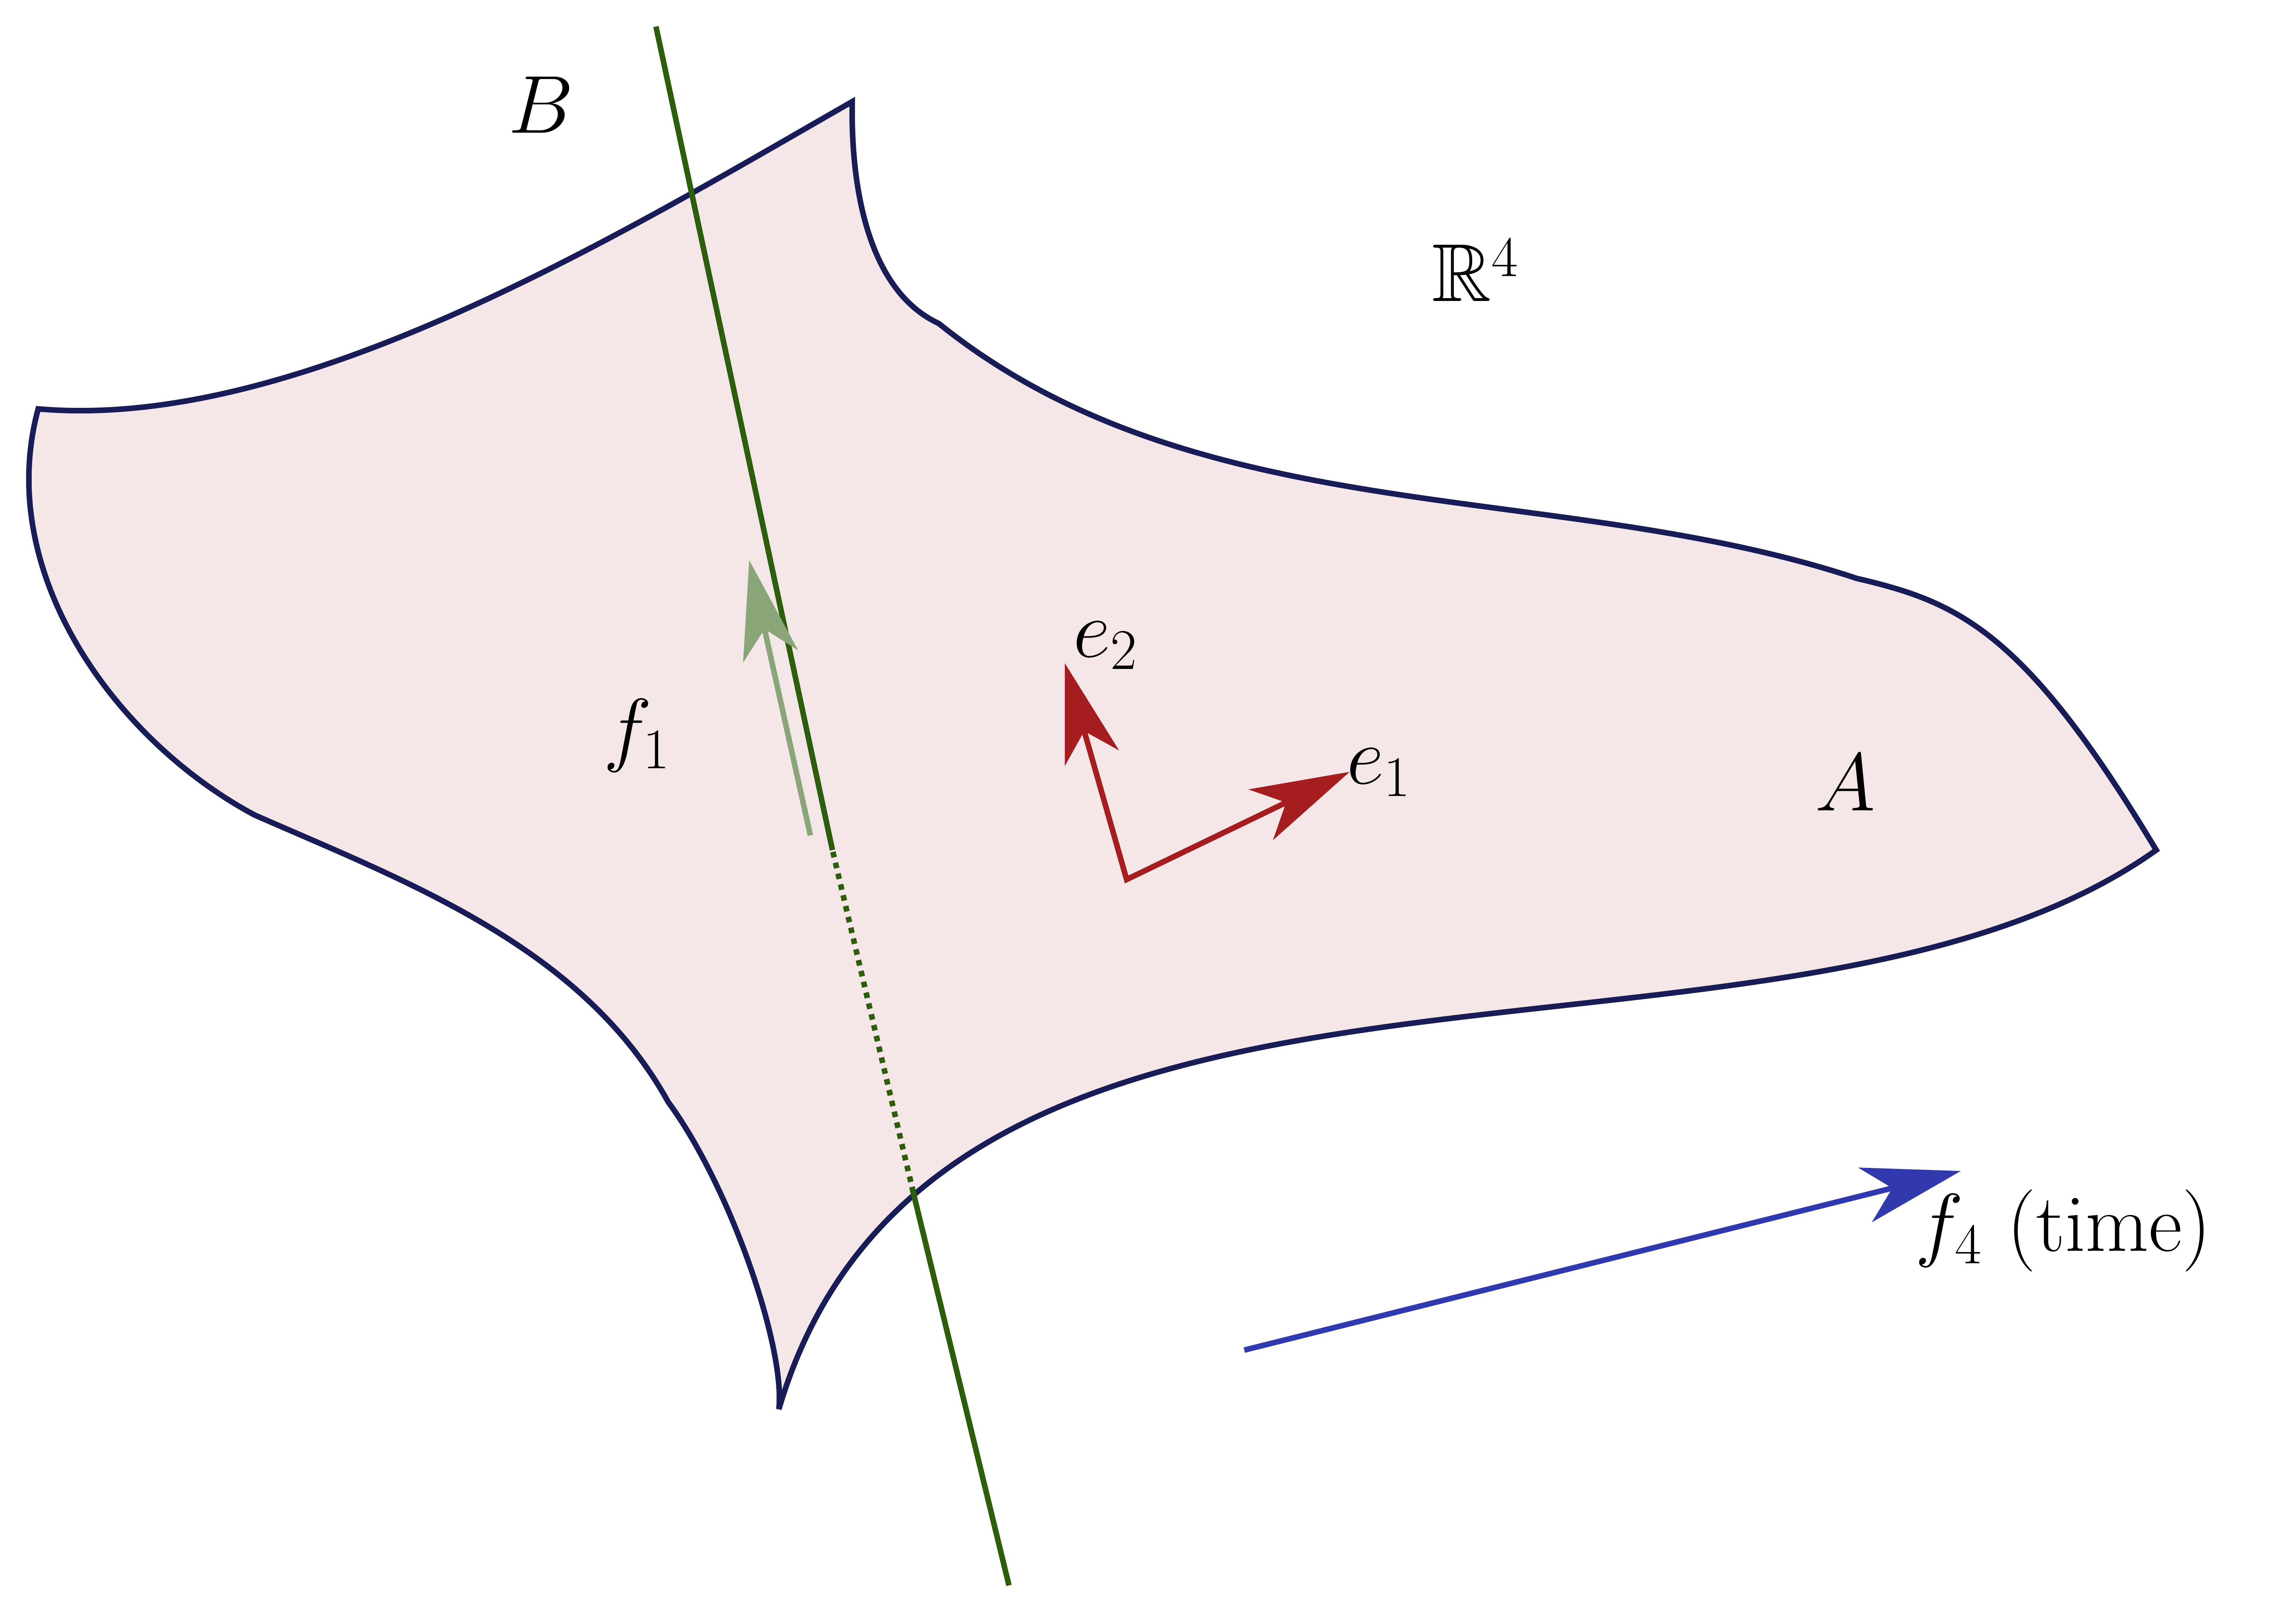
\includegraphics{figures/time_manifold_glitch_workaround.png}
\caption{Picking one basis element in the time direction}
\end{figure}

Here \(?\) is oriented in the ``forward time'' direction, and this is a
surface at time \(t=0\). Where \(A\cdot B = +1\), since
\(\left\{{ e_1, e_2, f_1, f_2 }\right\} = \left\{{ e_x, e_y, e_z, e_t }\right\}\)
is a oriented basis for \({\mathbb{R}}^4\). For \(?^2\), switching the
order of \(\alpha, \beta\) no longer yields an oriented basis, but in
this case it is \(?\) and \(A\cdot B = B \cdot A\). This is because
\begin{align*}
A \coloneqq
\begin{bmatrix}
0 &  1
\\
1 & 0 
\end{bmatrix}
\implies \det(A)
=-1 &&
\det 
\begin{bmatrix}
A &  
\\
 & A 
\end{bmatrix}
 = 1
.\end{align*}

\end{remark}

\begin{remark}

Let \(M^{2n}\) be an oriented manifold, then the cup product yields a
bilinear map
\(H^n(M; {\mathbb{Z}}) \otimes H^n(M; {\mathbb{Z}}) \to {\mathbb{Z}}\)
which is symmetric when \(n\) is odd and antisymmetric (or symplectic)
when \(n\) is even. This is a \textbf{perfect} (or \textbf{unimodular})
pairing (potentially after modding out by torsion) which realizes an
isomorphism:
\begin{align*}
\qty{ H^n(M; {\mathbb{Z}})/{\operatorname{tors}}}^\vee&\xrightarrow{\sim} H^n(M; {\mathbb{Z}})/{\operatorname{tors}}\\
\alpha \smile{-}&\mapsfrom \alpha
,\end{align*}
where the LHS are linear functionals on cohomology.

\end{remark}

\begin{remark}

Recall the universal coefficients theorem:
\begin{align*}
H^i(X; {\mathbb{Z}})/{\operatorname{tors}}\cong \qty{ H_i(X; {\mathbb{Z}})/{\operatorname{tors}}}^\vee
.\end{align*}
The general theorem shows that
\(H^i(X; {\mathbb{Z}})_{\operatorname{tors}}= H_{i-1}(X; {\mathbb{Z}})_{\operatorname{tors}}\).

\end{remark}

\begin{remark}

Note that if \(M\) is an oriented 4-manifold, then

\begin{center}
\begin{tikzcd}
    && {\operatorname{tors}}& {\text{torsionfree}} &&&&& {\operatorname{tors}}& {\text{torsionfree}} \\
    {H^0} && 0 & {\mathbb{Z}}&&& {H_0} && 0 & {\mathbb{Z}}\\
    {H^1} && 0 & \textcolor{rgb,255:red,214;green,92;blue,92}{{\mathbb{Z}}^{\beta_1}} &&& {H_1} && A & \textcolor{rgb,255:red,214;green,92;blue,214}{{\mathbb{Z}}^{\beta_1}} \\
    {H^2} && A & \textcolor{rgb,255:red,92;green,92;blue,214}{{\mathbb{Z}}^{\beta_2}} & {} & {{}} & {H_2} && A & \textcolor{rgb,255:red,92;green,92;blue,214}{{\mathbb{Z}}^{\beta_2}} \\
    {H^3} && A & \textcolor{rgb,255:red,214;green,92;blue,214}{{\mathbb{Z}}^{\beta_1}} &&& {H_3} && 0 & \textcolor{rgb,255:red,214;green,92;blue,92}{{\mathbb{Z}}^{\beta_1}} \\
    {H^4} && 0 & {\mathbb{Z}}&&& {H_4} && 0 & {\mathbb{Z}}
    \arrow["PD", from=4-5, to=4-6]
\end{tikzcd}
\end{center}

In particular, if \(M\) is simply connected, then
\(H_1(M) = {\mathsf{Ab}}(\pi_1(M)) = 0\), which forces \(A = 0\) and
\(\beta_1 = 0\).

\end{remark}

\begin{definition}[Lattice]

A \textbf{lattice} is a finite-dimensional free
\({\mathbb{Z}}{\hbox{-}}\)module \(L\) together with a symmetric
bilinear form
\begin{align*}
\cdot: L^{\otimes 2} &\to {\mathbb{Z}}\\
\ell \otimes m &\mapsto \ell \cdot m
.\end{align*}
The lattice \((L, \cdot)\) is \textbf{unimodular} if and only if the
following map is an isomorphism:
\begin{align*}
L &\to L^\vee\\
\ell &\mapsto \ell \cdot ({-})
.\end{align*}

\end{definition}

\begin{remark}

How to determine if a lattice is unimodular: take a basis
\(\left\{{ e_1, \cdots, e_n }\right\}\) of \(L\) and form the \emph{Gram
matrix}
\(M_{ij} \coloneqq( e_i \cdot e_j) \in \operatorname{Mat}(n\times n, {\mathbb{Z}})^{\operatorname{Sym}}\).
Then \((L, \cdot)\) is unimodular if and only if \(\det(M) = \pm 1\) if
and only if \(M ^{-1}\) is integral. In this case, the rows of
\(M ^{-1}\) will form a basis of the dual basis.

\end{remark}

\begin{definition}[Index of a lattice]

The \textbf{index} of a lattice is
\({\left\lvert { \det M} \right\rvert}\).

\end{definition}

\begin{exercise}[?]

Prove that
\({\left\lvert {\det M} \right\rvert} = {\left\lvert { L^\vee/ L } \right\rvert}\).

\end{exercise}

\begin{remark}

In general, for \(M^{4k}\), the \(H^{2k}/{\operatorname{tors}}\) is
unimodular. For \(M^{4k+2}\), the \(H^{2k+1}/{\operatorname{tors}}\) is
a unimodular \emph{symplectic} lattice, which is obtained by replacing
the word ``symmetric'' with ``antisymmetric'' everywhere above.

\end{remark}

\begin{example}[?]

For the torus, since the dimension is \(2 \pmod 4\), you get the
skew-symmetric matrix
\begin{align*}
\begin{bmatrix}
0  & 1
\\
-1 & 0
\end{bmatrix}
.\end{align*}

\todo[inline]{Check!}

\end{example}

\begin{definition}[Nondegenerate lattices]

A lattice is \textbf{nondegenerate} if \(\det M \neq 0\).

\end{definition}

\begin{definition}[Base change of lattices]

The tensor product \(L \otimes_{\mathbb{Z}}{\mathbb{R}}\) is a vector
space with an \({\mathbb{R}}{\hbox{-}}\)valued symmetric bilinear form.
This allows extending the lattice from \({\mathbb{Z}}^n\) to
\({\mathbb{R}}^n\).

\end{definition}

\begin{remark}

If \((L, \cdot)\) is nondegenerate, then Gram-Schmidt will yield an
orthonormal basis \(\left\{{ v_i }\right\}\). The number of positive
norm vectors is an invariant, so we obtain \({\mathbb{R}}^{p, q}\) where
\(p\) is the number of \(+1\)s in the Gram matrix and \(q\) is the
number of \(-1\)s. The \textbf{signature} of \((L, {-})\) is \((p, q)\),
or by abuse of notation \(p-q\). This is an invariant of the 4-manifold,
as is the lattice itself \(H^2(X; {\mathbb{Z}})/{\operatorname{tors}}\)
equipped with the intersection form.

\end{remark}

\begin{remark}

There is a perfect pairing called the \textbf{linking pairing}:

\begin{align*}
H^i(X; {\mathbb{Q}}/{\mathbb{Z}}) \otimes H^{n-i-1}(X; {\mathbb{Q}}/{\mathbb{Z}}) \to {\mathbb{Q}}/{\mathbb{Z}}
.\end{align*}

\begin{figure}
\centering
\resizebox{\columnwidth}{!}{%
\begin{tikzpicture}
\fontsize{44pt}{1em} 
\node (node_one) at (0,0) { \import{/home/zack/SparkleShare/github.com/Notes/Class_Notes/2021/Spring/FourManifolds/sections/figures}{2021-02-03_14-43.pdf_tex} };
\end{tikzpicture}
}
\end{figure}

\end{remark}

\begin{remark}

\(A \cdot B \coloneqq\sum_{p\in A \cap B} \operatorname{sgn}_p(A, B)\),
where \(A \pitchfork B\) and this turns out to be equal to the cup
product. This works for topological manifolds -- but there are no
tangent spaces there, so taking oriented bases doesn't work so well! You
can also view
\begin{align*}
[A] \smile[\omega] = \int_A \omega
.\end{align*}

\end{remark}

\hypertarget{friday-february-05}{%
\section{Friday, February 05}\label{friday-february-05}}

\begin{remark}

Recall that a lattice is \textbf{unimodular} if the map
\(L\to L^\vee\coloneqq\mathop{\mathrm{Hom}}(L, {\mathbb{Z}})\) is an
isomorphism, where \(\ell \mapsto \ell \cdot ({-})\). To check this, it
suffices to check if the Gram matrix \(M\) of a basis
\(\left\{{e_i}\right\}\) satisfies
\({\left\lvert { \det M } \right\rvert} = 1\).

\end{remark}

\begin{example}[Determinant 1 Integer Matrices]

The matrices \([1]\) and \([-1]\) correspond to the lattice
\({\mathbb{Z}}e\) where either \(e^2 \coloneqq e\cdot e = 1\) or
\(e^2 = -1\). If \(M_1, M_2\) both have absolute determinant \(1\), then
so does
\begin{align*}
\begin{bmatrix}
M_1 & 0 
\\
0 & M_2
\end{bmatrix}
.\end{align*}

So if \(L_1, L_2\) are unimodular, then taking an orthogonal sum
\(L_1 \oplus L_2\) also yields a unimodular lattice. So this yields
diagonal matrices with \(p\) copies of \(+1\) and \(q\) copies of
\(-1\). This is referred to as \(rm{1}_{p, q}\), and is an \emph{odd}
unimodular lattice of signature \((p, q)\) (after passing to
\({\mathbb{R}}\)). Here \emph{odd} means that there exists a \(v\in L\)
such that \(v^2\) is odd.

\end{example}

\begin{example}[Even unimodular lattices]

An even lattice must have no vectors of odd norm, so all of the diagonal
elements are in \(2{\mathbb{Z}}\). This is because
\((\sum n_i e_i)^2 = \sum_i n_i^2 e_i^2 + \sum_{i<j} 2 n_i, n_j e_i \cdot e_j\).
Note that the matrix must be symmetric, and one example that works is
\begin{align*}
\begin{bmatrix}
0 & 1 
\\
1 & 0
\end{bmatrix}
.\end{align*}
We'll refer to this lattice as \(H\), sometimes referred to as the
\emph{hyperbolic cell} or \emph{hyperbolic plane}.

\end{example}

\begin{example}[A harder even unimodular lattice]

This is built from the \(E_8\) Dynkin diagram:

\begin{center}
\begin{tikzcd}
    &&&& {\bullet_{e_8}} \\
    {\bullet_{e_7}} & {\bullet_{e_6}} & {\bullet_{e_5}} & {\bullet_{e_4}} & {\bullet_{e_3}} & {\bullet_{e_2}} & {\bullet_{e_1}}
    \arrow[no head, from=2-1, to=2-2]
    \arrow[no head, from=2-2, to=2-3]
    \arrow[no head, from=2-3, to=2-4]
    \arrow[no head, from=2-4, to=2-5]
    \arrow[no head, from=2-5, to=1-5]
    \arrow[no head, from=2-5, to=2-6]
    \arrow[no head, from=2-6, to=2-7]
\end{tikzcd}
\end{center}

The rule here is
\begin{align*}
e_i \cdot e_j = 
\begin{cases}
-2  & i =  j
\\
1 & e_i \to e_j \\
0 & \text{if not connected}.
\end{cases}
\end{align*}
So for example, \(e_2 \cdot e_6 = 0, e_1 \cdot e_3 = 1, e_2^2 = -2\).
You can check that \(\det(e_i \cdot e_j) = 1\), and this is referred to
as the \(E_8\) lattice. This is of signature \((0, 8)\), and it's
negative definite if and only if \(v^2 < 0\) for all \(v\neq 0\). One
can also negate the intersection form to define \(-E_8\). Note that any
simply-laced Dynkin diagram yields some lattice. For example, \(E_{10}\)
is unimodular of signature \((1, 9)\), and it turns out that
\(E_{10} \cong E_8 \oplus H\).

\end{example}

\begin{definition}[Unimodular lattice II]

Take
\begin{align*} 
\mathbf{II}_{a, a+8b} \coloneqq\bigoplus_{i=1}^a H \oplus \bigoplus_{j=1}^b E_8 
,\end{align*}
which is an even unimodular lattice since the diagonal entries are all
\(-2\), and using the fact that the signature is additive, is of
signature \((a, a+8b)\). Similarly,
\begin{align*} 
\mathbf{II}_{a+8b, a} \coloneqq\bigoplus_{i=1}^a H \oplus \bigoplus_{j=1}^b (-E_8) 
,\end{align*}
which is again even and unimodular.

\end{definition}

\begin{remark}

Thus

\begin{itemize}
\tightlist
\item
  \(\mathbf{I}_{p, q}\) is odd, unimodular, of signature \((p, q)\).
\item
  \(\mathbf{II}_{p, q}\) is even, unimodular, of signature \((p, q)\)
  only for \(p \equiv q \pmod 8\).
\end{itemize}

\end{remark}

\begin{theorem}[Serre]

Every unimodular lattice which is not positive or negative definite is
isomorphic to either \(\mathbf{I}_{p, q}\) or \(\mathbf{II}_{p, q}\)
with \(8\bigm|p-q\).

\end{theorem}

\begin{remark}

So there are obstructions to the existence of even unimodular lattices.
Other than that, the number of (say) positive definite even unimodular
lattices is

\begin{longtable}[]{@{}ll@{}}
\toprule
Dimension & Number of Lattices \\
\midrule
\endhead
8 & 1: \(E_8\) \\
16 & 2: \(E_8^{\oplus 2}, D_{16}^+\) \\
24 & 24: The Neimeir lattices (e.g.~the Leech lattice) \\
32 & \textgreater{}\(8\times 10^{16}\)!!!! \\
\bottomrule
\end{longtable}

Note that the signature of a definite lattice must be divisible by 8.

\end{remark}

\begin{remark}

There is an isometry: \(f: E_8 \to E_8\) where \(f\in O(E_8)\), the
linear maps preserving the intersection form (i.e.~the Weyl group
\(W(E_8)\), given by \(v\mapsto v + (v, e_i) e_i\). The Leech lattice
also shows up in the sphere packing problems for dimensions
\(2,4,8,24\). See Hale's theorem / Kepler conjecture for dimension 3!
This uses an identification of \(L\) as a subset of \({\mathbb{R}}^n\),
namely \(L \otimes_{\mathbb{Z}}{\mathbb{R}}\cong {\mathbb{R}}^{24}\) for
example, and the map \(L \hookrightarrow({\mathbb{R}}^{24}, \cdot)\) is
an isometric embedding into \({\mathbb{R}}^n\) with the standard form.
Connection to classification of Lie groups: root lattices.

\end{remark}

\begin{remark}

If \(M^4\) is a compact oriented 4-manifold and if the intersection form
on \(H^2(M; {\mathbb{Z}})\) is indefinite, then the only invariants we
can extract from that associated lattice are

\begin{itemize}
\tightlist
\item
  Whether it's even or odd, and
\item
  Its signature
\end{itemize}

If the lattice is even, then the signature satisfies \(8\bigm|p-q\). So
Poincaré duality forces unimodularity, and then there are further
number-theoretic restrictions. E.g. this prohibits \(\beta_2 =7\), since
then the signature couldn't possibly be 8 if the intersection form is
even.

\end{remark}

\hypertarget{characteristic-classes}{%
\subsection{Characteristic Classes}\label{characteristic-classes}}

\begin{definition}[Classifying space]

Let \(G\) be a topological group, then a \textbf{classifying space}
\(EG\) is a contractible topological space admitting a free continuous
\(G{\hbox{-}}\)action with a ``nice'' quotient.

\end{definition}

\begin{remark}

Thus there is a map \(EG \to BG \coloneqq EG/G\) which has the structure
of a principal \(G{\hbox{-}}\)bundle.

\begin{figure}
\centering
\resizebox{\columnwidth}{!}{%
\begin{tikzpicture}
\fontsize{40pt}{1em} 
\node (node_one) at (0,0) { \import{/home/zack/SparkleShare/github.com/Notes/Class_Notes/2021/Spring/FourManifolds/sections/figures}{2021-02-05_14-37.pdf_tex} };
\end{tikzpicture}
}
\end{figure}

Here we use a point \(p\) depending on \(U\) in an orbit to identify
orbits \(g\cdot p\) with \(g\), and we want to take transverse slices to
get local trivializations of \(U\in BG\). It suffices to know where
\(\pi ^{-1} (U) \cong U \times G\), and it suffices to consider
\(U \times\left\{{e}\right\}\). Moreover, \(EG\to BG\) is a universal
principal \(G{\hbox{-}}\)bundle in the sense that if \(P\to X\) is a
universal \(G{\hbox{-}}\)bundle, there is an \(f:X\to BG\).

\begin{center}
\begin{tikzcd}
    P && EG \\
    \\
    X && BG
    \arrow[from=1-1, to=3-1]
    \arrow["f", from=3-1, to=3-3]
    \arrow[from=1-3, to=3-3]
    \arrow[dashed, from=1-1, to=1-3]
\end{tikzcd}
\end{center}

\begin{quote}
\href{https://q.uiver.app/?q=WzAsNCxbMCwyLCJYIl0sWzIsMCwiRUciXSxbMiwyLCJCRyJdLFswLDAsIlAiXSxbMywwXSxbMCwyLCJmIl0sWzEsMl0sWzMsMSwiIiwyLHsic3R5bGUiOnsiYm9keSI6eyJuYW1lIjoiZGFzaGVkIn19fV1d}{Link
to Diagram}
\end{quote}

Here bundles will be classified by homotopy classes of \(f\), so
\begin{align*}
\left\{{\text{Principal $G{\hbox{-}}$bundles} {}_{/ X} }\right\} \rightleftharpoons[X, BG]
.\end{align*}

\end{remark}

\begin{warnings}

This only works for paracompact Hausdorff spaces! The line
\({\mathbb{R}}\) with the doubled origin is a counterexample, consider
complex line bundles.

\end{warnings}

\todo[inline]{Revisit this last section, had to clarify a few things for myself!}

\hypertarget{monday-february-08}{%
\section{Monday, February 08}\label{monday-february-08}}

Last time: \(BG\) and \(EG\). See Milnor and Stasheff.

\begin{example}[?]

Let
\(G \coloneqq\operatorname{GL}_n({\mathbb{R}}) = {\mathbb{R}}^{\times}\),
then we can take
\begin{align*}
EG = {\mathbb{R}}^{\infty } \coloneqq\left\{{ (a_1, a_2, \cdots ) {~\mathrel{\Big|}~}a_i \in {\mathbb{R}}, a_{i\gg 0} = 0, a_i \text{ not all zero } }\right\}
.\end{align*}
Then \({\mathbb{R}}^{\times}\) acts on \(EG\) by scaling, and we can
take the quotient
\({\mathbb{R}}^{\infty } \setminus\left\{{0}\right\}/ {\mathbb{R}}^{\times}\),
where \(\mathbf{a} \sim \lambda \mathbf{a}\) for all
\(\lambda \in {\mathbb{R}}^{\times}\). This yields
\({\mathbb{RP}}^{\infty }\) as the quotient. You can check that \(E_G\)
is contractible: it suffices to show that
\(S^{\infty } \coloneqq\left\{{ \sum {\left\lvert {a_i} \right\rvert} = 1 }\right\}\)
is contractible. This works by decreasing the last nonzero coordinate
and increasing the first coordinate correspondingly. Moreover, local
lifts exist, so we can identify
\({\mathbb{RP}}^{\infty } \cong B{\mathbb{R}}^{\times}= BG\). Similarly
\(BC^{\times}\cong {\mathbb{CP}}^{\infty }\) with
\(E{\mathbb{C}}^{\times}\coloneqq{\mathbb{C}}^{\infty } \setminus\left\{{0}\right\}\).

\end{example}

\begin{example}[?]

Consider \(G = \operatorname{GL}_n({\mathbb{R}})\). It turns out that
\(BG = {\operatorname{Gr}}(d, {\mathbb{R}}^{\infty })\), which is the
set of linear subspaces of \({\mathbb{R}}^{\infty }\) of dimension
\(d\). This is spanned by \(d\) vectors \(\left\{{e_ i}\right\}\) in
some large enough \({\mathbb{R}}^N \subseteq {\mathbb{R}}^{\infty }\),
since we can take \(N\) to be the largest nonvanishing coordinate and
include all of the vectors into \({\mathbb{R}}^{\infty }\) by setting
\(a_{> N} = 0\). For any
\(L \in {\operatorname{Gr}}_d({\mathbb{R}}^{\infty })\), since
\({\mathbb{R}}^d\) has a standard basis, there is a natural
\(\operatorname{GL}_d\) torsor: the set of ordered bases of linear
subspaces. So define
\begin{align*}
EG \coloneqq\left\{{ \text{bases of linear subspaces } L \in {\operatorname{Gr}}_d({\mathbb{R}}^{\infty }) }\right\}
,\end{align*}
then any \(A\in \operatorname{GL}_d({\mathbb{R}})\) acts on \(EG\) by
sending
\((L, \left\{{e_i}\right\}) \mapsto (L, \left\{{ Le_i}\right\} )\). We
can identify \(EG\) as \(d{\hbox{-}}\)tuples of linearly independent
elements of \({\mathbb{R}}^{\infty }\), and there is a map
\begin{align*}
EG &\to BG \\
\left\{{e_i}\right\} &\mapsto {\operatorname{span}}_{\mathbb{R}}\left\{{e_i}\right\}
.\end{align*}
Thus there is a universal vector bundle over \(BGL_d\):

\begin{center}
\begin{tikzcd}
\mathcal{E}_L \coloneqq L 
  \ar[r] 
& 
\mathcal{E} 
  \ar[d] 
\\
& 
BGL_d
\end{tikzcd}
\end{center}

So \(\mathcal{E} \subseteq BGL_d \times{\mathbb{R}}^{\infty }\), where
we can define
\(\mathcal{E} \coloneqq\left\{{(L, p) {~\mathrel{\Big|}~}p\in L}\right\}\).
In this case, \(EG = \mathop{\mathrm{Frame}}( \mathcal{E})\) is the
frame bundle of this universal bundle. The same setup applies for
\(G \coloneqq\operatorname{GL}_d({\mathbb{C}})\), except we take
\({\operatorname{Gr}}_d({\mathbb{C}}^{\infty })\).

\end{example}

\begin{example}[?]

Consider \(G = O_d\), the set of orthogonal transformations of
\({\mathbb{R}}^d\) with the standard bilinear form, and \(U_d\) the set
of unitary such transformations. To be explicit:
\begin{align*}
U_d \coloneqq\left\{{ A \in \operatorname{Mat}(d \times d, {\mathbb{C}}) {~\mathrel{\Big|}~}{\left\langle {Av},~{Av} \right\rangle} = {\left\langle {v},~{v} \right\rangle} }\right\}
,\end{align*}
where
\begin{align*}
{\left\langle { {\left[ {v_1, \cdots, v_n} \right]}},~{{\left[ {v_1, \cdots, v_n } \right]} } \right\rangle} = \sum {\left\lvert {v_i} \right\rvert}^2
.\end{align*}
Alternatively, \(A^t A = I\) for \(O_d\) and
\({\overline{{A^t}}} A = I\) for \(U_d\). In this case,
\(BO_d = {\operatorname{Gr}}_d( {\mathbb{R}}^{\infty } )\) and
\(BU_d = {\operatorname{Gr}}_d( {\mathbb{C}}^{ \infty })\), but we'll
make the fibers smaller: set the fiber over \(L\) to be
\begin{align*}
(EO_d)_L \coloneqq\left\{{ \text{orthogonal frames of } L }\right\}
\end{align*}
and similarly \((EU_d)_L\) the unitary frames of \(L\). That there are
related comes from the fact that \(\operatorname{GL}_d\) retracts onto
\(O_d\) using the Gram-Schmidt procedure.

\end{example}

\begin{remark}

Recall that there is a bijective correspondence
\begin{align*}
\left\{{\substack{
  \text{Principal $G{\hbox{-}}$ bundles}
  \\ \text{on } X
}}\right\}
&\rightleftharpoons
  [X, BG]
\end{align*}
and there is also a correspondence
\begin{align*}
\left\{{\substack{
  \text{Principal $\operatorname{GL}_d{\hbox{-}}$bundles }\\
  \text{on } X
}}\right\}
&\rightleftharpoons
\left\{{\substack{
  \text{Principal ${\mathcal{O}}_d{\hbox{-}}$bundles } \\
  \text{on } X
}}\right\}
\end{align*}
Using the associated bundle construction, on the LHS we obtain vector
bundles \(\mathcal{E}\to X\) of rank \(d\), and on the RHS we have
bundles with a metric. In local trivializations
\(U \times{\mathbb{R}}^d \to {\mathbb{R}}^d\), the metric is the
standard one on \({\mathbb{R}}^d\). This is referred to as a
\textbf{reduction of structure group}, i.e.~a principal
\(\operatorname{GL}_d\) bundle admits possibly different trivializations
for which the transition functions lie in the subgroup \(O_d\).

\end{remark}

\begin{example}[?]

Given any trivial principal \(G{\hbox{-}}\)bundle, it has a reduction of
structure group to the trivial group. But the fact that the bundle is
trivial may not be obvious.

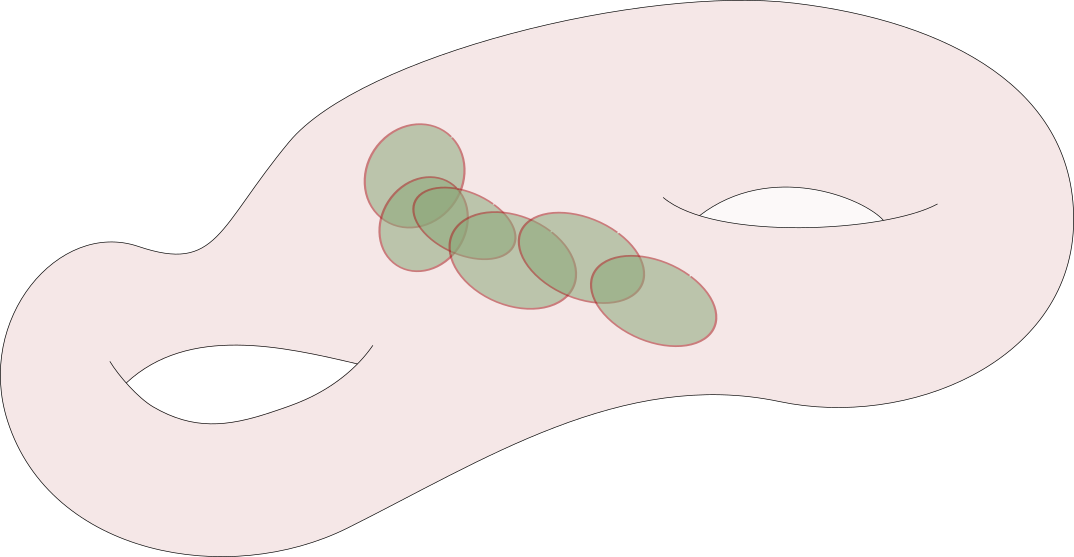
\includegraphics{figures/forbidden_donut.png}

\end{example}

\begin{remark}

We want to compute \(H^*(BU_d; {\mathbb{Z}})\). Why is this important?
Given any complex vector bundle \(\mathcal{E}\to X\) there is an
associated principal \(U_d\) bundle by choosing a metric, so we get a
homotopy class \([X, BU_d]\). Given any \(f\in [X, BU_d]\) and any
\(\alpha\in H^k(BU_d; {\mathbb{Z}})\), we can take the pullback
\(f^* \alpha \in H^k(X; {\mathbb{Z}})\), which are \textbf{Chern
classes}.

\end{remark}

\begin{exercise}[?]

Show that \(H^*(BU_d; {\mathbb{Z}})\) stabilizes as \(d\to \infty\) to
an infinitely generated polynomial ring
\({\mathbb{Z}}[c_1, c_2, \cdots]\) with each \(c_i\) in cohomological
degree \(2i\), so \(c_i \in H^{2i}(BU_d, {\mathbb{Z}})\).

\end{exercise}

\begin{definition}[?]

There is a map \(BU_{d-1} \to BU_d\), which we can identify as
\begin{align*}
{\operatorname{Gr}}_{d-1}(C^{\infty }) &\to {\operatorname{Gr}}_d({\mathbb{C}}^{\infty }) \\
\left\{{v_1, \cdots, v_{d-1}}\right\} &\mapsto {\operatorname{span}}\left\{{ (1, 0, 0, \cdots), sv_1, \cdots, sv_{d-1} }\right\}
.\end{align*}
This is defined by sending a basis where
\(s: {\mathbb{C}}^{\infty } \to {\mathbb{C}}^{\infty}\) is the map that
shifts every coordinate to the right by one.

\todo[inline]{
  Question: does ${\operatorname{Gr}}_d({\mathbb{C}}^{\infty})$ deformation retract onto the image of this map?
}

This will yield a fiber sequence
\begin{align*}
S^{2d-1} \to BU_{d-1} \to BU_d
\end{align*}
and using connectedness of the sphere and the LES in homotopy this will
identify
\begin{align*}
H^*(BU_d) = H^*(BU_{d-1})[c_d] && \text{where } c_d \in H^{2d}(BU_d)
.\end{align*}
The \textbf{Chern class} of a vector bundle \(\mathcal{E}\) , denoted
\(c_k( \mathcal{E} )\), will be defined as the pullback \(f^* c_k\).

\end{definition}

\hypertarget{wednesday-february-10}{%
\section{Wednesday, February 10}\label{wednesday-february-10}}

\begin{theorem}[?]

As \(n\to \infty\), we have
\begin{align*}
H^*(BO_n, {\mathbb{Z}}/2{\mathbb{Z}}) = {\mathbb{Z}}/2{\mathbb{Z}}[w_1, w_2, \cdots]
&& w_i \in H^i
.\end{align*}

\end{theorem}

\begin{definition}[Stiefel-Whitney class]

Given any principal \(O_n{\hbox{-}}\)bundle \(P\to X\), there is an
induced map \(X \xrightarrow{f} BO_n\), so we can pull back the above
generators to define the \textbf{Stiefel-Whitney classes} \(f^* w_i\).

\end{definition}

\begin{remark}

If \(P \coloneqq\mathop{\mathrm{OFrame}}TX\), then \(f^* w_1\) measures
whether \(X\) has an orientation, i.e.~\(f^* w_1 = 0 \iff X\) can be
oriented. We also have \(f^* w_i(P) = w_i( \mathcal{E} )\) where
\(P = \mathop{\mathrm{OFrame}}( \mathcal{E} )\). In general, we'll just
write \(w_i\) for Stiefel-Whitney classes and \(c_i\) for Chern classes.

\end{remark}

\begin{definition}[Pontryagin Classes]

The \textbf{Pontryagin classes} of a real vector bundle \(\mathcal{E}\)
are defined as
\begin{align*}
p_i( \mathcal{E} ) = (-1)^i c_{2i}( \mathcal{E} \otimes_{\mathbb{R}}{\mathbb{C}})
.\end{align*}
Note that the complexified bundle above is a complex vector bundle with
the same transition functions as \(\mathcal{E}\), but has a reduction of
structure group from \(\operatorname{GL}_n({\mathbb{C}})\) to
\(\operatorname{GL}_n({\mathbb{R}})\).

\end{definition}

\begin{observation}

\({\mathbb{RP}}^{\infty }\) and \({\mathbb{CP}}^{\infty }\) are examples
of \(K(\pi, n)\) spaces, which are the unique-up-to-homotopy spaces
defined by
\begin{align*}
\pi_k K (\pi, n) = 
\begin{cases}
\pi &  k=n
\\
0 & \text{else}.
\end{cases}
\end{align*}

\end{observation}

\begin{theorem}[Brown Representability]

\begin{align*}
H^n(X; \pi) \cong [X, K( \pi, n) ]
.\end{align*}

\end{theorem}

\begin{example}[?]

\begin{align*}
[X, {\mathbb{RP}}^{\infty } ] &\cong H^1(X; {\mathbb{Z}}/2{\mathbb{Z}}) \\
[X, {\mathbb{CP}}^{\infty } ] &\cong H^2(X; {\mathbb{Z}})
.\end{align*}

\end{example}

\begin{proposition}[?]

There is a correspondence
\begin{align*}
\left\{{\substack{
  \text{Complex line bundles}
}}\right\}
\rightleftharpoons
[X, {\mathbb{CP}}^{\infty }] = [X, BC^{\times}]
\rightleftharpoons
H^2(X; {\mathbb{Z}})
\end{align*}
Importantly, note that for \(X \in {\mathsf{Mfd}}_{\mathbb{C}}\),
\(H^2(X; {\mathbb{Z}})\) measures \emph{smooth} complex line bundles and
not holomorphic bundles.

\end{proposition}

\begin{proof}[?]

We'll take an alternate direct proof. Consider the exponential exact
sequence on \(X\):
\begin{align*}
0 \to \underline{Z} \to {\mathcal{O}}\xrightarrow{\exp} {\mathcal{O}}^{\times}
.\end{align*}
Note that \(\underline{{\mathbb{Z}}}\) consists of locally constant
\({\mathbb{Z}}{\hbox{-}}\)valued functions, \({\mathcal{O}}\) consists
of smooth functions, and \({\mathcal{O}}^{\times}\) are ???.

\todo[inline]{Can't read screenshot! :(}

This yields a LES in homology:

\begin{center}
\begin{tikzcd}
    {H^0(X; \underline{{\mathbb{Z}}})} && {H^0(X; {\mathcal{O}})} && {H^0(X; {\mathcal{O}}^{\times})} \\
    \\
    {H^1(X; \underline{{\mathbb{Z}}})} && \textcolor{rgb,255:red,214;green,92;blue,92}{H^1(X; {\mathcal{O}})} && {H^1(X; {\mathcal{O}}^{\times})} \\
    \\
    {H^2(X; \underline{{\mathbb{Z}}})} && \textcolor{rgb,255:red,214;green,92;blue,92}{H^2(X; {\mathcal{O}})} && {H^2(X; {\mathcal{O}}^{\times})}
    \arrow[from=1-1, to=1-3]
    \arrow[from=1-3, to=1-5]
    \arrow[from=1-5, to=3-1, out=0, in=180]
    \arrow[from=3-1, to=3-3]
    \arrow[from=3-3, to=3-5]
    \arrow[from=3-5, to=5-1, out=0, in=180]
    \arrow[from=5-1, to=5-3]
    \arrow[from=5-3, to=5-5]
\end{tikzcd}
\end{center}

\begin{quote}
\href{https://q.uiver.app/?q=WzAsOSxbMCwwLCJIXjAoWDsgXFxjb25zdGFudHtcXFpafSkiXSxbMCwyLCJIXjEoWDsgXFxjb25zdGFudHtcXFpafSkiXSxbMCw0LCJIXjIoWDsgXFxjb25zdGFudHtcXFpafSkiXSxbMiwwLCJIXjAoWDsgXFxPTykiXSxbMiwyLCJIXjEoWDsgXFxPTykiLFswLDYwLDYwLDFdXSxbMiw0LCJIXjIoWDsgXFxPTykiLFswLDYwLDYwLDFdXSxbNCwwLCJIXjAoWDsgXFxPT1xcdW5pdHMpIl0sWzQsMiwiSF4xKFg7IFxcT09cXHVuaXRzKSJdLFs0LDQsIkheMihYOyBcXE9PXFx1bml0cykiXSxbMCwzXSxbMyw2XSxbNiwxXSxbMSw0XSxbNCw3XSxbNywyXSxbMiw1XSxbNSw4XV0=}{Link
to Diagram}
\end{quote}

Since \({\mathcal{O}}\) admits a partition of unity,
\(H^{>0}(X; {\mathcal{O}}) = 0\) and all of the red terms vanish. For
complex line bundles \(L\),
\(H^1(X, {\mathcal{O}}^{\times}) \cong H^2(X; {\mathbb{Z}})\). Taking a
local trivialization
\({ \left.{{L}} \right|_{{U}} } \cong U \times{\mathbb{C}}\), we obtain
transition functions
\begin{align*}
t_{UV} \in C^{\infty }(U \cap V, \operatorname{GL}_1({\mathbb{C}}) )
\end{align*}
where we can identify
\(\operatorname{GL}_1({\mathbb{C}}) \cong {\mathbb{C}}^{\times}\). We
then have
\begin{align*}
(t_{U_{ij}}) \in \prod_{i < j} {\mathcal{O}}^{\times}(U_i \cap U_j) = C^1(X; {\mathcal{O}}^{\times})
.\end{align*}
Moreover,
\begin{align*}
\qty{ 
t_{U_{ij}}
t_{U_{ik}} ^{-1}
t_{U_{jk}}
}_{i,j,k} 
= {{\partial}}( t_{U_{ij} } ) _{i, j} = 0
,\end{align*}
since transitions functions satisfy the cocycle condition. So in fact
\((t_{U_{ij}}) \in Z^1(X; {\mathcal{O}}^{\times}) = \ker {{\partial}}^1\),
and we can take its equivalence class
\([ ( t_{U_{ij} } ) ] \in H^1(X; {\mathcal{O}}^{\times}) = \ker {{\partial}}^1 / \operatorname{im}{{\partial}}^0\).
Changing trivializations by some
\(s_i \in \prod_i {\mathcal{O}}^{\times}(U_i)\) yields a composition
which is a different trivialization of the same bundle:

\begin{center}
\begin{tikzcd}
    {{ \left.{{L}} \right|_{{U_i}} }} && {U_i \times{\mathbb{C}}} &&& {U_i \times{\mathbb{C}}}
    \arrow["{h_i}", from=1-1, to=1-3]
    \arrow["{\cdot s_i}", from=1-3, to=1-6]
    \arrow[curve={height=30pt}, from=1-1, to=1-6]
\end{tikzcd}
\end{center}

\begin{quote}
\href{https://q.uiver.app/?q=WzAsMyxbMCwwLCJcXHJve0x9e1VfaX0iXSxbMiwwLCJVX2kgXFxjcm9zcyBcXENDIl0sWzUsMCwiVV9pIFxcY3Jvc3MgXFxDQyJdLFswLDEsImhfaSJdLFsxLDIsIlxcY2RvdCBzX2kiXSxbMCwyLCIiLDIseyJjdXJ2ZSI6NX1dXQ==}{Link
to Diagram}
\end{quote}

So the \((t_{ U_{ij}}\) change \emph{exactly} by an
\({{\partial}}^0( s_i)\). Thus the following map is well-defined:
\begin{align*}
L \mapsto [ (t_{U_{ij}} ) ] \in H^1(X; {\mathcal{O}}^{\times})
.\end{align*}

There is another construction of the map
\begin{align*}
\left\{{L}\right\} &\to H^2(X; {\mathbb{Z}}) \\
L &\mapsto c_1(L)
.\end{align*}
Take a smooth section of \(L\) and \(s\in H^0(X; L)\) that intersects an
\({\mathcal{O}}{\hbox{-}}\)section of \(L\) transversely. Then
\begin{align*}
V(s) \coloneqq\left\{{ x\in X {~\mathrel{\Big|}~}s(x) = 0 }\right\}
\end{align*}
is a submanifold of real codimension 2 in \(X\), and
\(c_1(L) = [ V(s) ] \in H^2(X; {\mathbb{Z}})\).

\end{proof}

\begin{theorem}[Splitting Principle for Complex Vector Bundles]

\envlist

\begin{enumerate}
\def\labelenumi{\arabic{enumi}.}
\item
  Suppose that \(\mathcal{E} = \bigoplus_{i=1}^r L_i\) and let
  \(c(\mathcal{E}) \coloneqq\sum c_i(\mathcal{E}\). Then
  \begin{align*}
    c(\mathcal{E}) = \prod_{i=1}^r \qty{ 1 + c_i (L_i) }
    .\end{align*}
\item
  Given any vector bundle \(\mathcal{E} \to X\), there exists some \(Y\)
  and a map \(Y\to X\) such that
  \(f^*: H^k(X; {\mathbb{Z}}) \hookrightarrow H^k(Y; {\mathbb{Z}})\) is
  injective and \(f^* \mathcal{E} = \bigoplus_{i=1}^r L_i\).
\end{enumerate}

\end{theorem}

\begin{slogan}

To verify any identities on characteristic classes, it suffices to prove
them in the case where \(\mathcal{E}\) splits into a direct sum of line
bundles.

\end{slogan}

\begin{example}[?]

\begin{align*}
c( \mathcal{E} \oplus \mathcal{F}) = c( \mathcal{E} ) c( \mathcal{F} )
.\end{align*}
To prove this, apply the splitting principle. Choose \(Y, Y'\) splitting
\(\mathcal{E}, \mathcal{E}'\) respectively, this produces a space \(Z\)
and a map \(f:Z\to X\) where both split. We can write
\begin{align*}
f^* \mathcal{E} &= \bigoplus L_i 
&& c(f^* \mathcal{E} ) = \prod \qty{ 1 + c_1(L_i) } \\
f^* \mathcal{F} &= \bigoplus M_j 
&& c(f^* \mathcal{E} ) = \prod \qty{ 1 + c_1(M_j) }
.\end{align*}

We thus have
\begin{align*}
c( f^* \mathcal{E} \oplus f^* \mathcal{F} ) 
&= \prod \qty{1 + c_1(L_i) } \qty{1 + c_1(M_j)} \\
&= c(f^* \mathcal{E} ) c(f^* \mathcal{F} )
,\end{align*}
and
\(f^* (c( \mathcal{E} \oplus \mathcal{F} ) = f^* (c (\mathcal{E}) c( \mathcal{F}))\).
Since \(f^*\) is injective, this yields the desired identity.

\end{example}

\begin{example}[?]

We can compute \(c(\operatorname{Sym}^2 \mathcal{E})\), and really any
tensorial combination involving \(\mathcal{E}\), and it will always
yield some formula in the \(c_i( \mathcal{E} )\).

\end{example}

\hypertarget{friday-february-12}{%
\section{Friday, February 12}\label{friday-february-12}}

\begin{remark}

Last time: the splitting principle. Suppose we have
\(\mathcal{E} = L_1 \oplus \cdots \oplus L_r\) and let
\(x_i \coloneqq c_i(L_i)\). Then \(c_k(\mathcal{E})\) is the degree
\(2k\) part of \(\prod_{i=1}^r (1 + x_i )\) where each \(x_i\) is in
degree \(2\). This is equal to \(e_k(x_1, \cdots, x_r)\) where \(e_k\)
is the \(k\)th elementary symmetric polynomial.

\end{remark}

\begin{example}[?]

For example,

\begin{itemize}
\item
  \(e_1 = x_1 + \cdots x_r\).
\item
  \(e_2 = x_1 x_2 + x_1 x_3 + \cdots = \sum_{i < j} x_i x_j\)
\item
  \(e_3 = \sum_{i<j<k} x_i x_j x_k\), etc.
\end{itemize}

\end{example}

\begin{remark}

The theorem is that any symmetric polynomial is a polynomial in the
\(e_i\). For example, \(p_2 = \sum x_i^2\) can be written as
\(e_1^2 - 2e_2\). Similarly,
\(p_3 = \sum x_i^3 = e_1^3 - 3e_1 e_2 -3e_3\) Note that the coefficients
of these polynomials are important for representations of \(S_n\), see
\emph{Schur polynomials}.

\end{remark}

\begin{remark}

Due to the splitting principle, we can pretend that \(x_i = c_i(L_i)\)
exists even when \(\mathcal{E}\) doesn't split. If
\(\mathcal{E} \to X\), the individual symbols \(x_i\) don't exist, but
we can write '
\begin{align*}
x_1^3 + \cdots + x_r^3 = e_1^3 - 3e_1 e_2 - 3e_3 \coloneqq c_1(\mathcal{E})^3 + 3c_1(\mathcal{E}) c_2(\mathcal{E}) + \cdots
,\end{align*}
which is a well-defined element of \(H^6(X; {\mathbb{Z}})\). So this
polynomial defines a characteristic class of \(\mathcal{E}\), and this
can be done for any symmetric polynomial. We can change basis in the
space of symmetric polynomials to now define different characteristic
classes.

\end{remark}

\begin{definition}[Chern Character]

The \textbf{Chern character} is defined as
\begin{align*}
\operatorname{ch}(\mathcal{E}) 
&\coloneqq\sum_{i=1}^r e^{x_i}\in H^*(X; {\mathbb{Q}}) \\
&\coloneqq\sum_{i=1}^r \sum_{k=0}^{\infty } {x_i^k \over k!} \\
&= \sum_{k=0}^{\infty } {p_k(x_1, \cdots, x_r) \over k!} \\
&= \operatorname{rank}(\mathcal{E}) + c_1(\mathcal{E}) + { c_1(\mathcal{E}) - c_2(\mathcal{E}) \over 2!} + { c_1(\mathcal{E})^3 - 3c_1(\mathcal{E}) c_2(\mathcal{E}) - 3 c_3(\mathcal{E}) \over 3!} + \cdots \\
& \qquad \in H^0 + H^2 + H^4 + H^6 \\
&=\operatorname{ch}_0(\mathcal{E}) + \operatorname{ch}_1(\mathcal{E}) + \operatorname{ch}_2( \mathcal{E} ) + \cdots, \\
&   \quad \operatorname{ch}_i(\mathcal{E}) \in H^{2i}(X; {\mathbb{Q}}) 
.\end{align*}

\end{definition}

\begin{definition}[Total Todd class]

The \textbf{total Todd class}
\begin{align*}
\mathrm{td}(\mathcal{E})
\coloneqq
\prod_{i=1}^r { x_i \over 1 - e^{-x_i} }
.\end{align*}

Note that
\begin{align*}
{x_i \over 1 - e^{-x_i} } = 1 + {x_i \over 2} + {x_i^2 \over 12} + {x_i^4 \over 720} + \cdots = 1 + {x_i \over 2} + \sum_{i=1}^{\infty } { (-1)^{i-1} B_i \over (2i)! } x^{2i}
.\end{align*}
where L'Hopital shows that the derivative at \(x_i = 0\) exists, so it's
analytic at zero and the expansion makes sense, and the \(B_i\) are
Bernoulli numbers.

\end{definition}

\begin{remark}[Very important and useful!!]

\(\operatorname{ch}(\mathcal{E} \oplus \mathcal{F}) = \operatorname{ch}(\mathcal{E}) + \operatorname{ch}(\mathcal{F})\)
and
\(\operatorname{ch}( \mathcal{E} \otimes\mathcal{F} ) = \sum_{i,j} e^{x_i + y_j} = \operatorname{ch}( \mathcal{E} ) \operatorname{ch}(\mathcal{F} )\)
using the fact that \(c_1(L_1 \otimes L_2) = c_1(L_1) c_1(L_2)\). So
\(\operatorname{ch}\) is a ``ring morphism'' in the sense that it
preserves multiplication \(\otimes\) and addition \(\oplus\), making the
Chern character even better than the total Chern class.

\end{remark}

\begin{definition}[Todd Class]

Let \(X \in {\mathsf{Mfd}}_{\mathbb{C}}\), then define the \textbf{Todd
class} of \(X\) as
\(\mathrm{td}_{\mathbb{C}}(X) \coloneqq\mathrm{td}(TX)\) where \(TX\) is
viewed as a complex vector bundle. If
\(X\in {\mathsf{Mfd}}_{\mathbb{R}}\), define
\(\mathrm{td}_{\mathbb{R}}= \mathrm{td}(TX \otimes_{\mathbb{R}}{\mathbb{C}})\).

\end{definition}

\hypertarget{section-5-riemann-roch-and-generalizations}{%
\subsection{Section 5: Riemann-Roch and
Generalizations}\label{section-5-riemann-roch-and-generalizations}}

\begin{remark}

Let \(X\in {\mathsf{Top}}\) and let \(\operatorname{\mathcal{F}}\) be a
sheaf of vector spaces. Suppose
\(h^i(X; \operatorname{\mathcal{F}}) \coloneqq\dim H^i(X; \operatorname{\mathcal{F}}) < \infty\)
for all \(i\) and is equal to 0 for \(i \gg 0\).

\end{remark}

\begin{definition}[Euler Characteristic of a Sheaf]

The \textbf{Euler characteristic} of \(\operatorname{\mathcal{F}}\) is
defined as
\begin{align*}
\chi(X; \operatorname{\mathcal{F}}) \coloneqq\chi(\operatorname{\mathcal{F}}) \coloneqq\sum_{i=0}^{\infty } (-1)^i h_i(X; \operatorname{\mathcal{F}} )
.\end{align*}

\end{definition}

\begin{warnings}

This is not always well-defined!

\end{warnings}

\begin{example}[?]

Let \(X\in {\mathsf{Mfd}}_{\text{cpt}}\) and take
\(\operatorname{\mathcal{F}} \coloneqq\underline{{\mathbb{R}}}\), we
then have
\begin{align*}
\chi(X; \underline{{\mathbb{R}}}) = h^0(X; {\mathbb{R}}) - h^1(X; {\mathbb{R}}) + \cdots = b_0 - b_1 + b_2 - \cdots \coloneqq\chi_{{\mathsf{Top}}}(X)
.\end{align*}

\end{example}

\begin{example}[?]

Let \(X = {\mathbb{C}}\) and take
\(\operatorname{\mathcal{F}} \coloneqq{\mathcal{O}}\coloneqq{\mathcal{O}}^{\text{holo}}\)
the sheaf of holomorphic functions. We then have
\(h^{> 0}(X; {\mathcal{O}}) = 0\), but \(H^0(X; {\mathcal{O}})\) is the
space of all holomorphic functions on \({\mathbb{C}}\), making
\(\dim_{\mathbb{C}}h^0(X; {\mathcal{O}})\) infinite.

\end{example}

\begin{example}[?]

Take \(X = {\mathbb{P}}^1\) with \({\mathcal{O}}\) as above,
\(h^0({\mathbb{P}}^1; {\mathcal{O}}) = 1\) since \({\mathbb{P}}^1\) is
compact and the maximum modulus principle applies, so the only global
holomorphic functions are constant. We can write
\({\mathbb{P}}^1 = {\mathbb{C}}_1 \cup{\mathbb{C}}_2\) as a cover and
\(h^i({\mathbb{C}}, {\mathcal{O}}) = 0\), so this is an acyclic cover
and we can use it to compute \(h^1({\mathbb{P}}^1; {\mathcal{O}})\)
using Čech cohomology. We have

\begin{itemize}
\item
  \(C^0({\mathbb{P}}^1; {\mathcal{O}}) = {\mathcal{O}}({\mathbb{C}}_1) \oplus {\mathcal{O}}({\mathbb{C}}_2)\)
\item
  \(C^1({\mathbb{P}}^1; {\mathcal{O}}) = {\mathcal{O}}({\mathbb{C}}_1 \cap{\mathbb{C}}_2) = {\mathcal{O}}({\mathbb{C}}^{\times})\).
\item
  The boundary map is given by
  \begin{align*}
  {\partial}_0: C^0 &\to C^1 \\
  ( f(z), g(z) ) &\mapsto g(1/z) - f(z)
  \end{align*}
  and there are no triple intersections.
\end{itemize}

Is every holomorphic function on \({\mathbb{C}}^{\times}\) of the form
\(g(1/z) - f(z)\) with \(f,g\) holomorphic on \({\mathbb{C}}\). The
answer is yes, by Laurent expansion, and thus \(h^1 = 0\). We can thus
compute \(\chi({\mathbb{P}}^1; {\mathcal{O}}) = 1-0 = 1\).

\end{example}

\hypertarget{monday-february-15}{%
\section{Monday, February 15}\label{monday-february-15}}

\begin{remark}

Last time: we saw that \(\chi({\mathbb{P}}^1, {\mathcal{O}}) = 1\), and
we'd like to generalize to holomorphic line bundles on a Riemann
surface. This will be the main ingredient for Riemann-Roch.

\end{remark}

\begin{theorem}[?]

Let \(X \in {\mathsf{Mfd}}_{\mathbb{C}}\) be compact and let
\(\mathcal{F}\) be a holomorphic vector bundle on \(X\) \footnote{Or
  more generally a finitely-generated \({\mathcal{O}}{\hbox{-}}\)module,
  i.e.~a coherent sheaf.} Then \(\chi\) is well-defined and
\begin{align*} h^{> \dim_{\mathbb{C}}X}(X; \mathcal{F} ) = 0.\end{align*}

\end{theorem}

\begin{remark}

The locally constant sheaf \(\underline{{\mathbb{C}}}\) is not an
\({\mathcal{O}}{\hbox{-}}\)module,
i.e.~\(\underline{{\mathbb{C}}}(U) \not\in {\mathsf{{\mathcal{O}}(U)}{\hbox{-}}\mathsf{Mod}}\).
In fact, \(h^{2i}(X, \underline{{\mathbb{C}}}) = {\mathbb{C}}\) for all
\(i\).

\end{remark}

\begin{proof}[?]

We'll can resolve \(\mathcal{F}\) as a sheaf by first mapping to its
smooth sections and continuing in the following way:
\begin{align*}
0 \to \mathcal{F} \to C^{\infty } \mathcal{F} \xrightarrow{\mkern 1.5mu\overline{\mkern-1.5mu{\partial}\mkern-1.5mu}\mkern 1.5mu} F \otimes A^{0, 1} \to \cdots
,\end{align*}
where
\(\mkern 1.5mu\overline{\mkern-1.5mu{\partial}\mkern-1.5mu}\mkern 1.5muf = \sum_i {\frac{\partial f}{\partial {\overline{{z}}}_i}\,} \, d{\overline{{z}}}_i\).
Suppose we have a holomorphic trivialization of
\({ \left.{{\mathcal{F} }} \right|_{{U}} } \cong {\mathcal{O}}_{U}^{\oplus r}\)
and we have sections
\((s_1, \cdots, s_r) \in C^{\infty } \mathcal{F}(U)\), which are smooth
functions on \(U\). In local coordinates we have
\begin{align*}
\mkern 1.5mu\overline{\mkern-1.5mu{\partial}\mkern-1.5mu}\mkern 1.5mus \coloneqq(\mkern 1.5mu\overline{\mkern-1.5mu{\partial}\mkern-1.5mu}\mkern 1.5mus_1, \cdots, \mkern 1.5mu\overline{\mkern-1.5mu{\partial}\mkern-1.5mu}\mkern 1.5mus_r)
,\end{align*}
but is this well-defined globally? Given a different trivialization over
\(V \subseteq X\), the \(s_i\) are related by transition functions, so
the new sections are \(t_{UV}(s_1, \cdots, s_r)\) where
\(t_{UV}: U \cap V \to \operatorname{GL}_r({\mathbb{C}})\). Since
\(t_{UV}\) are holomorphic, we have
\begin{align*}
\mkern 1.5mu\overline{\mkern-1.5mu{\partial}\mkern-1.5mu}\mkern 1.5mu( t_{UV} (s_1, \cdots, s_r)) = t_{UV} \mkern 1.5mu\overline{\mkern-1.5mu{\partial}\mkern-1.5mu}\mkern 1.5mu(s_1, \cdots, s_r)
.\end{align*}
This makes
\(\mkern 1.5mu\overline{\mkern-1.5mu{\partial}\mkern-1.5mu}\mkern 1.5mu: C^{\infty } \mathcal{F} \to F\otimes A^{0, 1}\)
a well-defined (but not \({\mathcal{O}}{\hbox{-}}\)linear) map. We can
thus continue this resolution using the Leibniz rule:

\begin{align*}
0 \to \mathcal{F} \to C^{\infty } \mathcal{F} \xrightarrow{\mkern 1.5mu\overline{\mkern-1.5mu{\partial}\mkern-1.5mu}\mkern 1.5mu} F \otimes A^{0, 1} \xrightarrow{\mkern 1.5mu\overline{\mkern-1.5mu{\partial}\mkern-1.5mu}\mkern 1.5mu} \cdots F \otimes A^{0, 2} \xrightarrow{\mkern 1.5mu\overline{\mkern-1.5mu{\partial}\mkern-1.5mu}\mkern 1.5mu} \cdots
,\end{align*}
which is an exact sequence of sheaves since
\((A^{0, {-}}, \mkern 1.5mu\overline{\mkern-1.5mu{\partial}\mkern-1.5mu}\mkern 1.5mu)\)
is exact.

\todo[inline]{Why? Split into line bundles?}

We can identify
\(C^{\infty }\operatorname{\mathcal{F}} = \operatorname{\mathcal{F}} \otimes A^{0, 0}\),
and \(\operatorname{\mathcal{F}} \otimes A^{0, q}\) is a smooth vector
bundle on \(X\). Using partitions of unity, we have that
\(\operatorname{\mathcal{F}} \otimes A^{0, q}\) is acyclic, so its
higher cohomology vanishes, and
\begin{align*}
H^i(X; \operatorname{\mathcal{F}} ) \cong 
\frac
{ \ker ( \mkern 1.5mu\overline{\mkern-1.5mu{\partial}\mkern-1.5mu}\mkern 1.5mu: \operatorname{\mathcal{F}}\otimes A^{0, i} \to \operatorname{\mathcal{F}} \otimes A^{0, i+1} }
{ \operatorname{im}( \mkern 1.5mu\overline{\mkern-1.5mu{\partial}\mkern-1.5mu}\mkern 1.5mu: \operatorname{\mathcal{F}}\otimes A^{0, i-1} \to \operatorname{\mathcal{F}} \otimes A^{0, i} }
.\end{align*}
However, we know that \(A^{0, p} = 0\) for all
\(p> n \coloneqq\dim_{\mathbb{C}}X\), since any wedge of \(p>n\) forms
necessarily vanishes since there are only \(n\) complex coordinates.

\end{proof}

\begin{warnings}

This only applies to holomorphic vector bundles or
\({\mathcal{O}}{\hbox{-}}\)modules!

\end{warnings}

\hypertarget{riemann-roch}{%
\subsection{Riemann-Roch}\label{riemann-roch}}

\begin{theorem}[Riemann-Roch]

Let \(C\) be a compact connected Riemann surface,
i.e.~\(X\in {\mathsf{Mfd}}_{\mathbb{C}}\) with
\(\dim_{\mathbb{C}}(X) = 1\), and let \(\mathcal{L}\to C\) be a
holomorphic line bundle. Then
\begin{align*}
\chi(C, \mathcal{L}) = \deg(L) + (1-g) && \text{where } \deg(L) \coloneqq\int_C c_1(\mathcal{L})
\end{align*}
and \(g\) is the genus of \(C\).

\end{theorem}

\begin{proof}[?]

We'll introduce the notion of a ``point bundle'', which are particularly
nice line bundles, denoted \({\mathcal{O}}(p)\) for
\(p\in {\mathbb{C}}\).

\begin{figure}
\centering
\resizebox{\columnwidth}{!}{%
\begin{tikzpicture}
\fontsize{34pt}{1em} 
\node (node_one) at (0,0) { \import{/home/zack/SparkleShare/github.com/Notes/Class_Notes/2021/Spring/FourManifolds/sections/figures}{2021-02-15_14-16.pdf_tex} };
\end{tikzpicture}
}
\end{figure}

Taking \({\mathbb{D}}\) to be a disc of radius \(1/2\) and \(V\) to be
its complement, we have
\(t_{uv}(z) = z^{-1}\in {\mathcal{O}}^*(U \cap V)\). We can take a
holomorphic section \(s_p \in H^0( C, {\mathcal{O}}(p) )\), where
\({ \left.{{s_p}} \right|_{{U}} } = z\) and
\({ \left.{{s_p}} \right|_{{V}} } = 1\). Then
\(t_{uv}( { \left.{{s_p}} \right|_{{U}} } ) = { \left.{{s_p}} \right|_{{V}} }\)
on the overlaps. We have a function which precisely vanishes to first
order at \(p\). Recall that \(c_1( {\mathcal{O}}(p) )\) is represented
by \([ V(s) ] = [p]\), and moreover
\(\int_C c_1 ( {\mathcal{O}}(p) ) = 1\). We now want to generalize this
to a \textbf{divisor}: a formal \({\mathbb{Z}}{\hbox{-}}\)linear
combination of points.

\begin{example}[?]

Take \(p, q,r\in C\), then a divisor can be defined as something like
\(D \coloneqq 2[p] - [q] + 3[r]\).

\end{example}

Define
\({\mathcal{O}}(D) \coloneqq\bigotimes_{i} {\mathcal{O}}(p_i)^{\otimes n_i}\)
for any \(D = \sum n_i [p_i]\). Here tensoring by negatives means taking
duals,
i.e.~\({\mathcal{O}}( -[p] ) \coloneqq{\mathcal{O}}^{\otimes_{-1}} \coloneqq{\mathcal{O}}(p)^\vee\),
the line bundle with inverted transition functions. \({\mathcal{O}}(D)\)
has a meromorphic section given by
\begin{align*}
s_D \coloneqq\prod s_{p_i}^{n_i} \in \operatorname{Mero}(C, {\mathcal{O}}(D) )
\end{align*}
where we take the sections coming from point bundles. We can compute
\begin{align*}
\int_C c_1 ( {\mathcal{O}}(D) ) = \sum n_i \coloneqq\deg(D)
.\end{align*}
.

\begin{example}[?]

\begin{align*}
\deg( 2[p] -[q] + 3[r]) = 4
.\end{align*}

\end{example}

\begin{remark}

Assume our line bundle \(L\) is \({\mathcal{O}}(D)\), we'll prove
Riemann-Roch in this case by induction on
\(\sum {\left\lvert {n_i} \right\rvert}\). The base case is
\({\mathcal{O}}\), which corresponds to taking an empty divisor. Then
either

\begin{itemize}
\tightlist
\item
  Take \(D = D_0 + [p]\) with
  \(\deg(D_0) < \sum {\left\lvert {n_i} \right\rvert}\) (for which we
  need some positive coefficient), or
\item
  Take \(D_0 = D + [p]\).
\end{itemize}

\end{remark}

\begin{claim}

There is an exact sequence
\begin{align*}
0 \to {\mathcal{O}}(D_0) &\to {\mathcal{O}}(D) \to {\mathbb{C}}_p \to 0\\
s\in {\mathcal{O}}(D_0)(U) &\mapsto s \cdot s_p \in {\mathcal{O}}( D_0 + [p] ) (U)
,\end{align*}
where the last term is the skyscraper sheaf at \(p\).

\end{claim}

\begin{proof}[?]

The given map is \({\mathcal{O}}{\hbox{-}}\)linear and injective, since
\(s_p\neq 0\) and \(s s_p=0\) forces \(s=0\). Recall that we looked at
\({\mathcal{O}}\xrightarrow{\cdot z} {\mathcal{O}}\) on
\({\mathbb{C}}\), and this section only vanishes at \(p\) (and to first
order). The same situation is happening here.

\end{proof}

Thus there is a LES

\begin{center}
\begin{tikzcd}
    &&&& 0 \\
    \\
    {H^0( {\mathcal{O}}(D_0) )} && {H^0( {\mathcal{O}}(D) )} && {H^0( {\mathcal{O}}({\mathbb{C}}_p) )} \\
    \\
    {H^1( {\mathcal{O}}(D_0) )} && {H^1( {\mathcal{O}}(D) )} && {H^1( {\mathcal{O}}({\mathbb{C}}_p) ) = 0} \\
    \\
    0
    \arrow[from=3-5, to=5-1, out=0, in=180]
    \arrow[from=3-1, to=3-3]
    \arrow[from=3-3, to=3-5]
    \arrow[from=5-1, to=5-3]
    \arrow[from=5-3, to=5-5]
    \arrow[from=1-5, to=3-1, out=0, in=180]
    \arrow[from=5-5, to=7-1, out=0, in=180]
\end{tikzcd}
\end{center}

\begin{quote}
\href{https://q.uiver.app/?q=WzAsOCxbMCwyLCJIXjAoIFxcT08oRF8wKSApIl0sWzIsMiwiSF4wKCBcXE9PKEQpICkiXSxbNCwyLCJIXjAoIFxcT08oXFxDQ19wKSApIl0sWzAsNCwiSF4xKCBcXE9PKERfMCkgKSJdLFsyLDQsIkheMSggXFxPTyhEKSApIl0sWzQsNCwiSF4xKCBcXE9PKFxcQ0NfcCkgKSA9IDAiXSxbNCwwLCIwIl0sWzAsNiwiMCJdLFsyLDNdLFswLDFdLFsxLDJdLFszLDRdLFs0LDVdLFs2LDBdLFs1LDddXQ==}{Link
to Diagram}
\end{quote}

We also have \(h^1({\mathbb{C}}_p) = 0\) by taking a sufficiently fine
open cover where \(p\) is only in one open set. So just checking Čech
cocycles yields
\(C_U^1(C, {\mathbb{C}}_p) \coloneqq\prod_{i<j} {\mathbb{C}}_p(U_i \cap U_j) = 0\)
since \(p\) is in no intersection.

\begin{figure}
\centering
\resizebox{\columnwidth}{!}{%
\begin{tikzpicture}
\fontsize{35pt}{1em} 
\node (node_one) at (0,0) { \import{/home/zack/SparkleShare/github.com/Notes/Class_Notes/2021/Spring/FourManifolds/sections/figures}{2021-02-15_14-38.pdf_tex} };
\end{tikzpicture}
}
\end{figure}

We obtain \(\chi( {\mathcal{O}}(D) = \chi( {\mathcal{O}}(D_0) ) + 1\),
using that it is additive in SESs
\begin{align*}
0 \to 
\operatorname{\mathcal{E}}_1 \to
\operatorname{\mathcal{E}}_2 \to
\operatorname{\mathcal{E}}_3 \to
0
\implies && 
\chi(\operatorname{\mathcal{E}}_2) = \chi( \operatorname{\mathcal{E_1}}) + \chi( \operatorname{\mathcal{E}}_3 )
\end{align*}
and thus
\begin{align*}
\int_C c_1 ({\mathcal{O}}(D) ) = \sum n_i = \deg(D) = \deg D_0 + 1
.\end{align*}
The last step is to show that \(\chi(C, {\mathcal{O}}) = 1-g\), so just
define \(g\) so that this is true!

\end{proof}

\begin{remark}

Why is every \(L \cong {\mathcal{O}}(D)\) for some \(D\)? Easy to see if
\(L\) has meromorphic sections: if \(s\) is a meromorphic section of
\(L\), then the following works:
\begin{align*}
D = \operatorname{Div}(s) = \sum_p {\operatorname{Ord}}_p(s) [p]
.\end{align*}
Then \({\mathcal{O}}\cong L\otimes{\mathcal{O}}(-D)\) has a meromorphic
section \(s s_{-D}\), a global nonvanishing section with
\(\operatorname{Div}(s s_{-D} ) = \emptyset\). Proving that every
holomorphic line bundle has a meromorphic section is hard!

\end{remark}

\hypertarget{friday-february-19}{%
\section{Friday, February 19}\label{friday-february-19}}

\hypertarget{applications-of-riemann-roch}{%
\subsection{Applications of
Riemann-Roch}\label{applications-of-riemann-roch}}

\begin{definition}[Curves]

A \textbf{curve} is a compact complex manifold of complex dimension 1.

\end{definition}

\begin{example}[?]

Let \(C\) be a curve, then \(\Omega_C^1\) is the sheaf of holomorphic
1-forms, and \(\Omega_C^{>1} = 0\). We also have the sheaves
\(A^{1, 0}, A^{0, 1}, A^{1, 1},\) the sheaves of smooth
\((p, q){\hbox{-}}\)forms. Here the only nonzero combinations are
\((0, 0), (0, 1), (1, 0), (1, 1)\) by dimensional considerations. Let
\(L\) be a holomorphic line bundle on \(C\), then
\begin{align*} \chi(C, L) = h^0(L) - h^1(L) = \deg(L) + 1 - g .\end{align*}

\end{example}

\begin{remark}

In general it can be hard to compute \(h^1(L)\), since this is sheaf
cohomology (sections over double overlaps, cocycle conditions, etc). On
the other hand, \(h^0\) is easy to understand, since
\(h^0( \Omega^1_C)\) is the dimension of the global holomorphic sections
\(H^0(C, L) = L(C)\). A key tool here is the following:

\end{remark}

\begin{proposition}[Serre Duality]

\begin{align*}
H^1(C, L) \cong H^0(C, L ^{-1} \otimes\Omega_C^1)^\vee
,\end{align*}
noting that these are both global sections of a line bundle.

\end{proposition}

\begin{proof}[?]

Recall that we had a resolution of the sheaf \(L\) given by by smooth
vector bundles:
\begin{align*}
0 \to L \hookrightarrow L\otimes A^{0, 0} \xrightarrow{\mkern 1.5mu\overline{\mkern-1.5mu{\partial}\mkern-1.5mu}\mkern 1.5mu} L \otimes A^{0, 1} \xrightarrow{\mkern 1.5mu\overline{\mkern-1.5mu{\partial}\mkern-1.5mu}\mkern 1.5mu} 0
.\end{align*}
So we know that
\begin{align*}
H^1(C, L) = H^0(L\otimes A^{0, 1}) / \mkern 1.5mu\overline{\mkern-1.5mu{\partial}\mkern-1.5mu}\mkern 1.5muH^0(L\otimes A^{0, 0})
.\end{align*}
Choose a Hermitian metric \(h\) on \(L\), i.e.~a map
\(h: L\otimes{\overline{{L}}} \to {\mathcal{O}}\). On fibers, we have
\(h_p: L_p \otimes\mkern 1.5mu\overline{\mkern-1.5mu L_p \mkern-1.5mu}\mkern 1.5mu \to {\mathbb{C}}\).
We'll also choose a metric on \(C\), say \(g\). Since \(C\) is a Riemann
surface, we have an associated volume form \(\nu\) on \(C\) (essentially
the determinant), so we can define a pairing between sections of
\(L\otimes A^{0, 0}\):
\begin{align*}
{\left\langle {s},~{t} \right\rangle} \coloneqq\int_C h(s, {\overline{{t}}} ) \,d\nu
.\end{align*}
Note that
\begin{align*}
{\left\langle {s},~{s} \right\rangle} = \int_C h(s, {\overline{{s}}}) \,d\nu \geq 0
&& \text{since }
h(s, {\overline{{s}}})(p) = 0 \iff s_p = 0
,\end{align*}
and moreover this integral is zero if and only if \(s=0\). So we have an
inner product on \(H^0(L\otimes A^{0, 0})\). We can also define a
pairing on sections of \(L\otimes A^{0, 1}\), say
\begin{align*}
{\left\langle { s \otimes \alpha},~{ t \otimes \beta} \right\rangle} = \int_C h(s, {\overline{{t}}}) \alpha\wedge {\overline{{\beta}}}
.\end{align*}
Note that \(h\) is a smooth function and
\(\alpha\wedge {\overline{{\beta}}}\) is a \((1, 1){\hbox{-}}\)form.
Moreover, this is positive and nondegenerate. We want to understand the
cokernel of the linear map
\begin{align*}
H^0(L \otimes A^{0, 0}) \xrightarrow{\mkern 1.5mu\overline{\mkern-1.5mu{\partial}\mkern-1.5mu}\mkern 1.5mu} H^0( L \otimes A^{0, 1})
.\end{align*}
To compute
\(\operatorname{coker}(\mkern 1.5mu\overline{\mkern-1.5mu{\partial}\mkern-1.5mu}\mkern 1.5mu)\),
we can look at the kernel of the adjoint, and it suffices to find the
orthogonal complement of
\(\operatorname{im}( \mkern 1.5mu\overline{\mkern-1.5mu{\partial}\mkern-1.5mu}\mkern 1.5mu)\),
i.e.~
\begin{align*}
\operatorname{coker}(\mkern 1.5mu\overline{\mkern-1.5mu{\partial}\mkern-1.5mu}\mkern 1.5mu) = \left\{{ t\in H^0(L\otimes A^{0, 1}) {~\mathrel{\Big|}~}{\left\langle {\mkern 1.5mu\overline{\mkern-1.5mu{\partial}\mkern-1.5mu}\mkern 1.5mus},~{t} \right\rangle} = 0 \, \forall s}\right\} 
.\end{align*}

\begin{figure}
\centering
\resizebox{\columnwidth}{!}{%
\begin{tikzpicture}
\fontsize{44pt}{1em} 
\node (node_one) at (0,0) { \import{/home/zack/SparkleShare/github.com/Notes/Class_Notes/2021/Spring/FourManifolds/sections/figures}{2021-02-19_14-18.pdf_tex} };
\end{tikzpicture}
}
\end{figure}

So we want to understand sections \(t\in H^0(L\otimes A^{0, 1})\) such
that
\begin{align*}
\int_C (\mkern 1.5mu\overline{\mkern-1.5mu{\partial}\mkern-1.5mu}\mkern 1.5mus){\overline{{t}}} = 0 && \forall s\in H^0(L\otimes A^{0, 0})
,\end{align*}
where \({{\partial}}C = \emptyset\). We'll basically want to do
integration by parts on this. Note that \(h(s, t) = hst\) here where we
view \(h\) as a certain section. Note that
\({\overline{{t}}} \in H^0({\overline{{L}}} \otimes A^{1, 0})\), so we
can replace \({\partial}\) with
\(d = \mkern 1.5mu\overline{\mkern-1.5mu{\partial}\mkern-1.5mu}\mkern 1.5mu+ {\partial}\)
and apply Stokes' theorem:
\begin{align*}
\int_C s d(h {\overline{{t}}}) &= 0 && \forall s\in H^0(L\otimes A^{0, 0}) \\
0 
&= \int_C s\mkern 1.5mu\overline{\mkern-1.5mu{\partial}\mkern-1.5mu}\mkern 1.5mu(h {\overline{{t}}}) \\
&= \int_C s {\mkern 1.5mu\overline{\mkern-1.5mu{\partial}\mkern-1.5mu}\mkern 1.5mu(h {\overline{{t}}}) \over d\nu}d\nu\\
&= {\left\langle {s},~{{\overline{{\mkern 1.5mu\overline{\mkern-1.5mu{\partial}\mkern-1.5mu}\mkern 1.5mu(h {\overline{{t}}}) \over d\nu }}}} \right\rangle}
\end{align*}
where \(h \in C^{\infty }(L ^{-1} \otimes{\overline{{L}}}^{-1})\) and
\(h{\overline{{t}}} \in C^{\infty }(L^{-1}\otimes A^{1, 0})\). But the
right-hand side is in \(H^0(L \otimes A^{0, 0} )\) and by nondegeneracy
we can conclude
\begin{align*}
{\overline{{\mkern 1.5mu\overline{\mkern-1.5mu{\partial}\mkern-1.5mu}\mkern 1.5mu(h {\overline{{t}}}) \over d\nu }}} = 0
\iff \mkern 1.5mu\overline{\mkern-1.5mu{\partial}\mkern-1.5mu}\mkern 1.5mu(h{\overline{{t}}}) = 0
.\end{align*}
We thus have \(h{\overline{{t}}} \in H^0( L ^{-1}\otimes A^{1, 0}\)
which is a holomorphic line bundle tensored with \(A^{0, 0}\). Thus
\(\operatorname{coker}(\mkern 1.5mu\overline{\mkern-1.5mu{\partial}\mkern-1.5mu}\mkern 1.5mu) \cong_h H^0( L ^{-1} \otimes\Omega^1)\).

\end{proof}

\begin{remark}

We showed
\({\left\langle {\mkern 1.5mu\overline{\mkern-1.5mu{\partial}\mkern-1.5mu}\mkern 1.5mus},~{t} \right\rangle} = {\left\langle {s},~{Y (t)} \right\rangle}\)
where \(Y\) is the adjoint given above. Then the kernel of \(Y\) wound
up being where
\(\mkern 1.5mu\overline{\mkern-1.5mu{\partial}\mkern-1.5mu}\mkern 1.5mu\)
vanishes, i.e.~holomorphic sections of a separate bundle. Here we had

\begin{itemize}
\tightlist
\item
  \(t \in H^0(L\otimes A^{0, 1})\)
\item
  \({\overline{{t}}} \in H^0({\overline{{L}}}\otimes A^{1,0})\)
\item
  \(h\in H^0( L ^{-1} \otimes{\overline{{ L ^{-1} }}})\)
\end{itemize}

\end{remark}

\hypertarget{monday-february-22}{%
\section{Monday, February 22}\label{monday-february-22}}

\begin{remark}

Last time: Serre duality, and we'll review Riemann-Roch. Recall that
this depended on the statement that every holomorphic line bundle
\(L\to C\) for \(C\) a complex curve is of the form
\(L = {\mathcal{O}}(D)\) for some divisor \(D\). Then
\begin{align*}
\chi(C, L) = h^0(L) - h^1(L) = \deg L + 1 - g, && \deg L = \int_C c_1(L)
,\end{align*}
Serre duality said that the space of sections \(H^1(C; L)\) is naturally
isomorphic to \(H^0(C, L ^{-1} \otimes\Omega_C^1)^\vee\). Notation:
given \(X \in {\mathsf{Mfd}}_{\mathbb{C}}^n\) of complex, dimension
\(n\), the \textbf{canonical bundle} is written
\(K_X \coloneqq\Omega_X^n\) and is the sheaf of holomorphic
\(n{\hbox{-}}\)forms. Serre duality will generalize: if
\(\mathcal{E}\to X\) is a holomorphic vector bundle, then
\(H^i(X; \mathcal{E}) \cong H^{n-i}(X; \mathcal{E}^\vee\otimes K_X)^\vee\).
Note that only \(H^0, H^1\) are the only nontrivial degrees for a curve.
For 4-manifolds, we'll have an \(H^2\) as well.

\end{remark}

\hypertarget{applications-of-riemann-roch-1}{%
\subsection{Applications of
Riemann-Roch}\label{applications-of-riemann-roch-1}}

\begin{proposition}[?]

There is a unique complex \(X\in {\mathsf{Mfd}}_{\mathbb{C}}\)
diffeomorphic to \(S^2\).

\end{proposition}

\begin{proof}[of proposition]

Note existence is clear, since we can take
\({\mathbb{CP}}^1 \coloneqq({\mathbb{C}}^2 \setminus\left\{{0}\right\}) / \mathbf{x} \sim \lambda\mathbf{x}\)
for \(\lambda\in {\mathbb{C}}^{\times}\), which is identified as the set
of complex lines through \(0\) in \({\mathbb{C}}^2\). This decomposes as
\({\mathbb{C}}\cup{\mathbb{C}}= \left\{{ [1, *] }\right\} \cup\left\{{ [*, 1] }\right\}\).
We now want to show that any two such complex manifolds are
biholomorphic. Let \(X \in {\mathsf{Mfd}}_{\mathbb{C}}^1\) with
\(X\cong_{C^{\infty }} S^2\), and consider for \(p\in X\) the point
bundle \({\mathcal{O}}(p) \to X\). The defining property was that there
exists a section \(s_p \in H^0(X; {\mathcal{O}}(p) )\) which vanishes at
first order at \(p\):

\begin{figure}
\centering
\resizebox{\columnwidth}{!}{%
\begin{tikzpicture}
\fontsize{43pt}{1em} 
\node (node_one) at (0,0) { \import{/home/zack/SparkleShare/github.com/Notes/Class_Notes/2021/Spring/FourManifolds/sections/figures}{2021-02-22_14-03.pdf_tex} };
\end{tikzpicture}
}
\end{figure}

We have
\begin{align*}
\chi(X; {\mathcal{O}}(p)) 
= \deg {\mathcal{O}}(p) + 1 - g(x) = 1 + 1 - 0 = 2
.\end{align*}

\begin{exercise}[?]

Check that \(\deg {\mathcal{O}}(p) = 1\).

\end{exercise}

On the other hand we have
\begin{align*}
\chi(X; {\mathcal{O}}(p)) 
=
h^0({\mathcal{O}}(p)) - h^1( {\mathcal{O}}(p) )
.\end{align*}

We have \(h^1( {\mathcal{O}}(p) ) = H60( K \otimes{\mathcal{O}}(-p)\),
and \(K_X = \Omega_X^1 = T^\vee X\), so the question is: what is the
degree of \(TX\) for \(X\cong S^2\)? We need to compute
\(\int_X c_1(TX)\). How many zeros does a vector field on the sphere
have? You can take the gradient vector field for a height function to
get \(2\), noting that the two zeros come in with a positive orientation

\begin{figure}
\centering
\resizebox{\columnwidth}{!}{%
\begin{tikzpicture}
\fontsize{44pt}{1em} 
\node (node_one) at (0,0) { \import{/home/zack/SparkleShare/github.com/Notes/Class_Notes/2021/Spring/FourManifolds/sections/figures}{2021-02-22_14-10.pdf_tex} };
\end{tikzpicture}
}
\end{figure}

In coordinates on \({\mathbb{CP}}^1\), the coordinate is given by \(z\)
and
\(z {\frac{\partial }{\partial z}\,} \mapsto -2 {\frac{\partial }{\partial w}\,}\)
for the coordinate \(w = 1/z\). We get \(\int_X c_1(TX) = 2\) and thus
\(\deg K_X = -2\) by dualizing.

\begin{fact}

\(\deg K_X = 2g-2\). Use the existence of a smooth vector field on
\(X\).

\end{fact}

\begin{lemma}[?]

If \(\deg L < 0\) on \(C\)\textless{} the \(h^0(C, L) = 0\).

\end{lemma}

\begin{proof}[?]

If \(s\in H^0(C, L)\) is nonzero, then since \(s\) is a holomorphic
section,
\begin{align*}
0 \leq \sum_{p\in C} {\operatorname{Ord}}_P (s) = \deg L
.\end{align*}

\end{proof}

By this lemma, \(h^1({\mathcal{O}}(p)) = 0\). We have
\(H^0(X; {\mathcal{O}}(p)) = {\mathbb{C}}s_p \oplus {\mathbb{C}}s\) for
our specific section \(s_p\) and some other section
\(s \neq \lambda s_p\). Note that \(s/s_p\) is a meromorphic section of
\({\mathcal{O}}(p) \times{\mathcal{O}}(-p) = {\mathcal{O}}\), so we have
a map
\begin{align*}
\varphi: {s \over s_p} : X\to {\mathbb{P}}^1
.\end{align*}
Note that \(P\mapsto \infty \in {\mathbb{P}}^1\) under this \(\varphi\),
and it's only the ratio that is well-defined. We have
\(\varphi ^{-1} (u) = \left\{{ s/s_p = u }\right\} = \left\{{ s - us_p =0 }\right\}\)
which is a single point. So \(\varphi\) is a degree 1 map, and \(X\) is
biholomorphic to \({\mathbb{P}}^1\) via \(\varphi\).

\end{proof}

\begin{remark}

So there is only one genus 0 Riemann surface. What about genus 1?

\begin{figure}
\centering
\resizebox{\columnwidth}{!}{%
\begin{tikzpicture}
\fontsize{44pt}{1em} 
\node (node_one) at (0,0) { \import{/home/zack/SparkleShare/github.com/Notes/Class_Notes/2021/Spring/FourManifolds/sections/figures}{2021-02-22_14-23.pdf_tex} };
\end{tikzpicture}
}
\end{figure}

By Riemann-Roch we know
\begin{align*}
\chi(C; {\mathcal{O}}) = \deg {\mathcal{O}}+ l - 1 = 0 = h^0({\mathcal{O}}) - h^1({\mathcal{O}})
.\end{align*}
We know \(h^0({\mathcal{O}}) = 1\) by the maximum modulus principle and
\(h^1(C; {\mathcal{O}}) = 1\). By Serre duality, \(h^0(C, K) = 1\), and
since \(\deg K = 2g-2 = 0\). So let \(s\in H^0(C, K)\) by a nonzero
section, which we know exists. We then get
\({\operatorname{Ord}}_p s = 0\) for all \(p\), so \(s\) vanishes
nowhere. But then we get an isomorphism of sheaves, since \(s\)
everywhere nonvanishing implies trivial cokernel:
\begin{align*}
{\mathcal{O}}\xrightarrow{\cdot s} K
.\end{align*}
So \(K_C = {\mathcal{O}}_C\) if \(g(C) = 1\), and such a Riemann surface
is an \textbf{elliptic curve}.

\end{remark}

\begin{example}[?]

Let \(C \coloneqq{\mathbb{C}}/ \Lambda\) for \(\Lambda\) some lattice.

\begin{figure}
\centering
\resizebox{\columnwidth}{!}{%
\begin{tikzpicture}
\fontsize{34pt}{1em} 
\node (node_one) at (0,0) { \import{/home/zack/SparkleShare/github.com/Notes/Class_Notes/2021/Spring/FourManifolds/sections/figures}{2021-02-22_14-28.pdf_tex} };
\end{tikzpicture}
}
\end{figure}

All transition functions are of the form \(z \mapsto z + \lambda\) for
some \(\lambda\in \Lambda\). What is a nonvanishing section of \(K_C\),
i.e.~a holomorphic one form \(\omega \coloneqq f(z) dz\) on
\({\mathbb{C}}\) that descends to \({\mathbb{C}}/\Lambda\). We would
need \(f(z)dz = f(z + \lambda)d(z+ \lambda)\) for all \(\lambda\).
Something like \(f=1\) works, so \(\omega= dz\) descends. In fact, \(f\)
must be constant, since
\(H^0( {\mathbb{C}}/ \Lambda, {\mathcal{O}}) = {\mathbb{C}}\,dz\) by the
maximum modulus principle. Now let \(p, q\in C\) and apply Riemann-Roch
to the line bundle \({\mathcal{O}}(p+q)\) yields
\begin{align*}
\chi( {\mathcal{O}}(p+q) ) &=
h^0( {\mathcal{O}}(p+q) )-
h^1( {\mathcal{O}}(-p-q) ) \\
&=
h^0( {\mathcal{O}}(p+q) )-0\\
&=
\deg {\mathcal{O}}(p+q)+1-1 \\
&=2
.\end{align*}
Thus there is a section \(s_{p+q} \in H^0( {\mathcal{O}}(p+q)) \ni s\)
that vanishes at \(p+q\), and similarly a map
\begin{align*}
{s\over s_{p+q}}: C \xrightarrow{\varphi} {\mathbb{P}}^1
.\end{align*}
We can check \(\varphi ^{-1} ( \infty ) = p+q\) and
\(\deg \varphi = 2\). Thus genus 1 surfaces have a generically 2-to-1
map to \({\mathbb{P}}^1\).

\begin{figure}
\centering
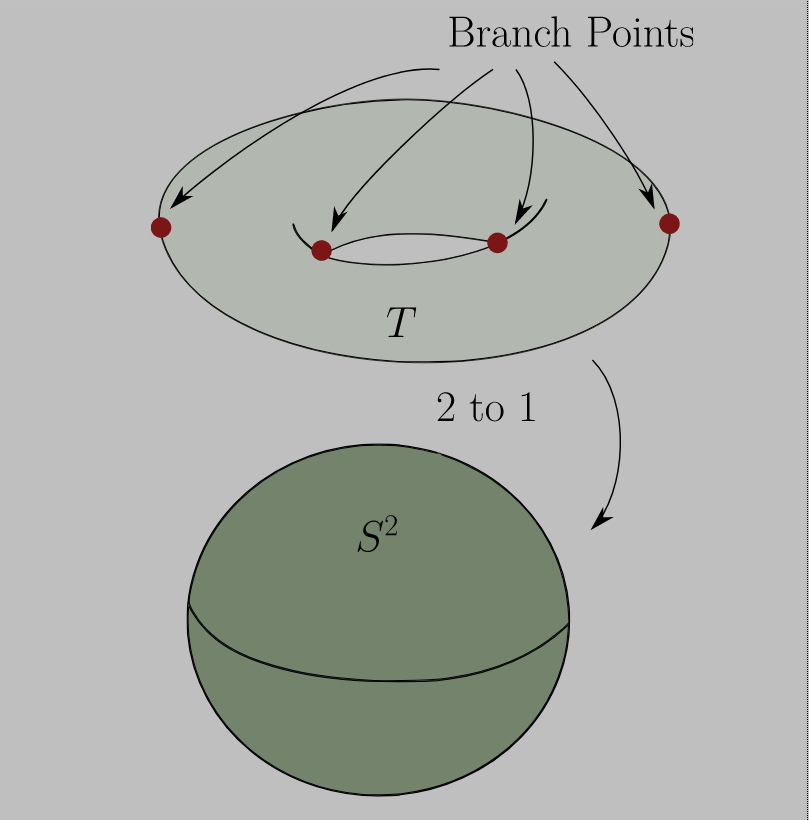
\includegraphics{figures/image_2021-02-25-20-41-53.png}
\caption{image\_2021-02-25-20-41-53}
\end{figure}

Note that homothetic lattices define an isomorphism between the elliptic
curves, and lattices mod homothety are in correspondence of elliptic
curves. By acting
\(\operatorname{PGL}_2(C) \curvearrowright{\mathbb{P}}^1\) since
\(\operatorname{GL}_2\) acts on lines since scaling an element fixes a
line. This is dimension 3. So elliptic curves are also in correspondence
with
\(\left\{{ 4 \text{ points on } {\mathbb{P}}^1}\right\} / \operatorname{PGL}_2({\mathbb{C}})\)
since this is now dimension 1. Note that by applying homothety, the two
basis vectors for a lattice can be rescaled so one is length 1 and the
other is a complex number \(\tau\), and we can identify this space with
\({\mathbb{H}}/ {\operatorname{SL}}_2({\mathbb{Z}})\).

\end{example}

\begin{exercise}[?]

Show that any \(g(C) = 2\) curve has a degree 2 map to
\({\mathbb{P}}^1\).

\end{exercise}

\begin{remark}

Similarly \(g(C) = 3\) are usually a curve of degree \(4\) in
\({\mathbb{CP}}^2\). Severi proof in the 50s: false! issues with
building moduli space for \(g\geq 23\). Need to use orbifold structure
to take into account automorphisms.

\end{remark}

\hypertarget{wednesday-february-24}{%
\section{Wednesday, February 24}\label{wednesday-february-24}}

Last time:
\begin{align*}
\chi(C, L) 
&= h^0(C, L) - h^1(C, L) \\
&= h^0(C, L) - h^0(C, L ^{-1} \otimes K_C) \\
&= \deg L + 1 -g
,\end{align*}
which is determined by purely topological information. We can generalize
this to arbitrary ranks of the bundle and arbitrary dimensions of
manifold:

\begin{theorem}[Hirzebruch-Riemann-Roch (HRR) Formula]

Let \(X\) be a compact complex manifold and let \(\mathcal{E} \to X\) be
a holomorphic vector bundle. Then
\begin{align*}
\chi( \mathcal{E} ) = \int_C \operatorname{ch}( \mathcal{E} ) \mathrm{td}(X)
.\end{align*}
The constituents here:

\begin{itemize}
\item
  The \textbf{Chern character}, summed over \(R\) the \emph{Chern
  roots}, which is in mixed cohomological degree.
  \begin{align*}
  \operatorname{ch}( \mathcal{E} ) \coloneqq\sum_{x_i \in R} e^{x_i} = \operatorname{ch}_0( \mathcal{E} ) + \operatorname{ch}_1( \mathcal{E} ) + \cdots + \operatorname{ch}_i( \mathcal{E} ) \in H^{2i}(X; {\mathbb{Q}})
  .\end{align*}
\item
  The \textbf{Todd class}, defined as
  \begin{align*}
  \mathrm{td}( F) \coloneqq\prod_{x_i \in R} {x_i \over 1 - e^{-x_i} }
  \end{align*}
  where \(\mathrm{td}(X) \coloneqq\mathrm{td}(TX)\) is viewed as a
  complex vector bundle, which is again in mixed cohomological degree.
\end{itemize}

\end{theorem}

\begin{remark}

Note that integrating over cohomology classes in mixed degree is just
equal to the integral over the top degree terms. Applying this to
\(X = C\) a curve and \(\mathcal{E} \coloneqq{\mathcal{O}}\), we obtain
\begin{align*}
\chi(C, {\mathcal{O}}) 
= \int_C \operatorname{ch}( {\mathcal{O}}) \mathrm{td}(C)
.\end{align*}

We have

\begin{itemize}
\item
  \(\operatorname{ch}({\mathcal{O}}) = e^{c_1({\mathcal{O}})} = e^0 = 1\)
\item
  \(\mathrm{td}(C) \coloneqq\mathrm{td}(TC) = c_1(TC) / (1- e^{ - c_1(TC) } )\),
  whose Taylor coefficients are the Bernoulli numbers. We can expand
  \(x/(1 -e^{-x}) = 1 + (x/2) + (x^2/12) - x^4(720) + \cdots\), and
  since terms above degree 2 vanish, we have
  \begin{align*}
  \cdots 
  &= \int_C 1 + \qty{ 1 + {c_1(TC) \over 2} } \\
  &= \int_C \qty{c_1(TC) \over 2 }\\
  &= {1\over 2} \chi_{\mathsf{Top}}(C) && \text{Chern-Gauss-Bonnet} \\
  &= {2-2g \over 2} \\
  &= 1-g
  .\end{align*}
\end{itemize}

We thus obtain
\begin{align*}
\chi(C, L) 
&= \int_C \operatorname{ch}(L) \mathrm{td}(C) \\
&= \int_C (1 + c_1(L) ) \qty {1 + {c_1(L) \over 2} }\\
&= \int_C c_1(L) + {c_1(TC) \over 2} \\
&= \deg L + 1-g
.\end{align*}

\end{remark}

\begin{remark}

Note that this is a better definition of genus than the previous one,
which was just the correction term in Riemann-Roch. Here we can define
it as \(g \coloneqq h^1/2\).

\end{remark}

\begin{exercise}[?]

Try to state and prove a Riemann-Roch formula for vector bundles on
curves.

\end{exercise}

\begin{proposition}[?]

Let \(S\) be a compact complex surface,
i.e.~\(S\in {\mathsf{Mfd}}_{\mathbb{C}}^2\). An example might be
\(C\times D\) for \(C,D\) two complex curves, or \({\mathbb{CP}}^2\).
Let \(L\to S\) be a holomorphic vector bundle. Then
\begin{align*}
\chi(L) = \chi({\mathcal{O}}_S) + {1\over 2} \qty{ L^2 - L \cdot K}
.\end{align*}
Note that \(L^2 \coloneqq\int_S c_1(L) c_1(L)\) is just shorthand for
taking the intersection of \(L\) with itself. Recall that
\(K \coloneqq\Omega_S^2\) is the space of holomorphic top forms.

\end{proposition}

\begin{proof}[?]

Let \(x_1, x_2\) be the Chern roots of \(TS\). By HRR, we have
\begin{align*}
\chi(L) 
&= \int_S \operatorname{ch}(L) \mathrm{td}(S) \\
&= \int_S \qty{ 1 + c_1(L) + {c_1(L)^2 \over 2!} } \qty{ {x_1 \over 1 - e^{-x_1} } {x_2 \over 1-e^{-x_2}} }\\
&= \int_S \qty{ 1 + c_1(L) + {c_1(L)^2 \over 2!} } \qty{1 + {x_1 \over 2} + {x_1^2 \over 12} }\qty{ 1 + {x_2 \over 2} + {x_2^2\over 12}} \\
&= \int_S \qty{ 1 + c_1(L) + {c_1(L)^2 \over 2!} } \qty{1 + {x_1 + x_2 \over 2} + {x_1^2 + x_2^2 + 3x_1 x_2 \over 12} } \\
&= \int_S \qty{ 1 + c_1(L) + {c_1(L)^2 \over 2!} } \qty{1 + {c_1(x_1, x_2) \over 2} + {c_1(x_1, x_2)^2 + c_2(x_1, x_2) \over 12 } } \\
&= \int_S \qty{ 1 + c_1(L) + {c_1(L)^2 \over 2!} } \qty{1 + { c_1(T) \over 2} + {c_1(T)^2 + c_2(T) \over 2 } } \\
&= \int_S {c_1(L)^2 \over 2} + {c_1(L) c_1(T) \over 2} + {c_1(T)^2 \over 2} + {c_2(T) \over 12} \quad \text{Take deg 4} \\
&= \int_S \qty{ c_1(L)^2 + c_1(L) c_1(T) \over 2} + \chi({\mathcal{O}}_S) \quad \text{HRR on last two terms}
.\end{align*}
where we've applied HRR to \({\mathcal{O}}_S\). It remains to show that
\(c_1(T) = -c_1(K)\). We have
\begin{align*}
K = \Omega_S^2 = \bigwedge\nolimits^2 T^\vee
.\end{align*}
Note that
\(\bigwedge\nolimits^{\text{top}} \mathcal{E} \coloneqq\det( \mathcal{E} )\)
for any bundle \(\mathcal{E}\) since this is a 1-dimensional bundle. We
have \(c_1(T) = -c_1(T^\vee)\) since the Chern roots of \(T^\vee\) are
\(-x_1, -x_2\). So it suffices to show \(c_1(T^\vee) = c_1(K)\), but
there is a general result that
\(c_1(\mathcal{E}) = c_1( \det \mathcal{E} )\). This uses the splitting
principle \(\mathcal{E} = \bigoplus_{i=1}^r L_i\) with
\(x_i = c_1(L_i)\). We have \(c_1(\mathcal{E}) = \sum x_i\) and
\(\det\mathcal{E} = \bigotimes_{i=1}^r L_i\), so
\(\sum x_i = c_1(L_1\otimes\cdots \otimes L_r)\).

\end{proof}

\begin{remark}

We want to use the following formula:
\begin{align*}
\chi(S, L) = \chi({\mathcal{O}}_S) = {1\over 2}(L^2 - L\cdot K)
.\end{align*}
This requires knowing \(\chi({\mathcal{O}}_S)\). Applying HRR yields
\begin{align*}
\chi({\mathcal{O}}_S) 
&= \int_S {c_1(T)^2 + c_2(T) \over 12}\\
&= \int_S { (-c_1(K))^2 + c_2(T) \over 12}\\
&= {K^2 + \displaystyle\int_S c_2(T) \over 12}
,\end{align*}
so we just need to understand \(\int_S c_2(T)\). But for
\(n=\operatorname{rank}\mathcal{E}\), \(c_n( \mathcal{E} )\) (the top
Chern class) is the fundamental class of a zero locus of a section of
\(\mathcal{E}\). Note that \(S \in {\mathsf{Mfd}}_{\mathbb{R}}^4\) is
oriented, so \(\int_S c_2(T)\) is the signed number of zeros of a smooth
vector field.

\begin{figure}
\centering
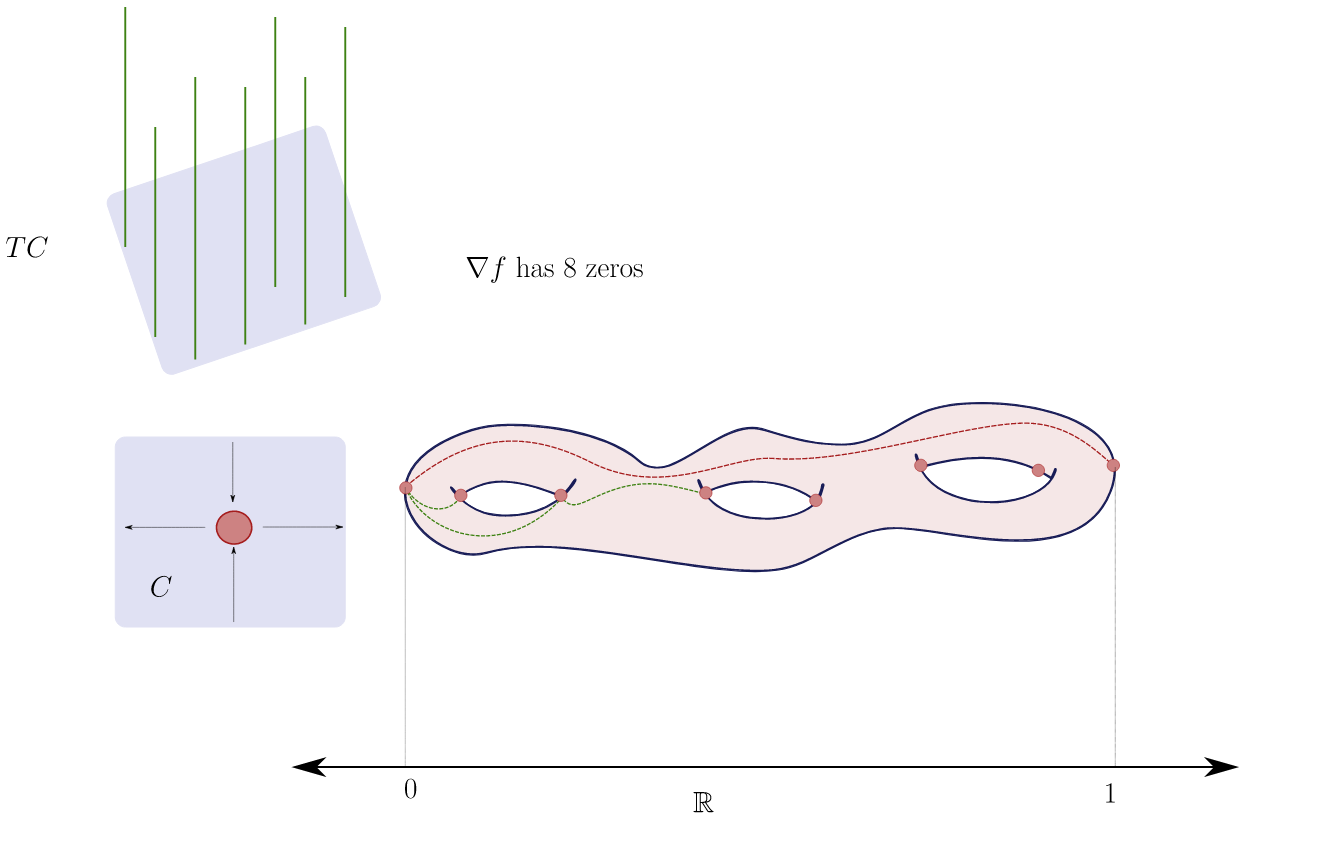
\includegraphics{figures/image_2021-02-25-20-42-49.png}
\caption{image\_2021-02-25-20-42-49}
\end{figure}

Looking at the tangent bundle of the surface, the local sign of an
intersection will be the number of incoming directions \(\pmod 2\),
i.e.~the index of the critical point. Then the signed number of zeros
here yields \(1-6+1 = -4 = \chi_{{\mathsf{Top}}}(C)\). More generally,
we have
\begin{align*}
\chi_{{\mathsf{Top}}}(M^n) = \int_C c_{n}(TM)
,\end{align*}
the \textbf{Chern-Gauss-Bonnet} formula. We can thus write
\begin{align*}
\chi({\mathcal{O}}_S) = {K^2 + \chi_{\mathsf{Top}}(S) \over 12 }
.\end{align*}

\end{remark}

\hypertarget{friday-february-26}{%
\section{Friday, February 26}\label{friday-february-26}}

\begin{remark}

Last time: Riemann-Roch for surfaces, today we'll discuss some examples.
Recall that if \(S \in {\mathsf{Mfd}}_{\mathbb{C}}^2\) is closed and
compact (noting that \(S\in {\mathsf{Mfd}}_{\mathbb{R}}^4\)) and
\(L\to S\) is a holomorphic line bundle then
\begin{align*}
\chi(S, L) = \chi({\mathcal{O}}_S) + {1\over 2}(L^2 - L \cdot K)
\end{align*}
where \(K = c_1(K_S)\) for \(K_S \coloneqq\Omega_S^2\) the canonical
bundle and \(L = c_1(L)\). We also saw
\begin{align*}
\chi({\mathcal{O}}_S) = {1\over 12}(K^2 + \chi_{{\mathsf{Top}}}(S))
,\end{align*}
where \(\chi_{\mathsf{Top}}\) is the Euler characteristic and is given
by
\begin{align*}
\chi_{\mathsf{Top}}(S) = 2 h^0(S; {\mathbb{C}}) - 2 h^1(S, {\mathbb{C}}) + h^2(S; {\mathbb{C}})
.\end{align*}

\end{remark}

\begin{example}[?]

Let \(S = {\mathbb{CP}}^2\), which can be given in local coordinates by
\begin{align*} 
\left\{{ [x_0: x_1: x_2 ] {~\mathrel{\Big|}~}(x_0, x_1, x_2) \in {\mathbb{C}}^3\setminus\left\{{0}\right\}}\right\} 
\end{align*}
where we only take equivalence classes of ratios
\([x,y,z] = [\lambda x, \lambda y, \lambda z]\) for any
\(\lambda\in {\mathbb{C}}^{\times}\). This decomposes as
\begin{align*}
{\mathbb{CP}}^2 \cup{\mathbb{C}}\cup\left\{{ {\operatorname{pt}}}\right\} = \left\{{ [1: x_1: x_2] }\right\} \cup\left\{{ [0 : x_1: x_2] }\right\} \cup\left\{{ [0:0:1] }\right\}
,\end{align*}
i.e.~we take \(x_0 \neq 0\), then \(x_0 = 0, x_1\neq 0\), then
\(x_0 = x_1 = 0\). Note that
\begin{align*}
h^i({\mathbb{CP}}^n; {\mathbb{Z}}) = 
\begin{cases}
{\mathbb{Z}}&  0 \leq i \leq 2n \text{ even} 
\\
0 & \text{else}.
\end{cases}
\end{align*}

We can use this to conclude that
\(\chi_{\mathsf{Top}}({\mathbb{CP}}^n) = n+1\) and
\(\chi_{\mathsf{Top}}({\mathbb{CP}}^2) = 3\). Over \({\mathbb{CP}}^n\)
we have a \textbf{tautological line bundle} \({\mathcal{O}}(-1)\) given
by sending each point to the corresponding line in
\({\mathbb{C}}^{n+1}\), i.e.~\({\mathcal{O}}(-1) \to {\mathbb{CP}}^n\)
given by
\begin{align*}
\lambda (x_0, \cdots, x_n) \mapsto [x_0: \cdots: x_n]
.\end{align*}
Note that the total space is
\(\mathop{\mathrm{Bl}}_0({\mathbb{C}}^{n+1})\) is the \textbf{blowup} at
zero, which separates the tangents at 0.

\end{example}

\begin{remark}

Let \(X\) be an algebraic variety, i.e.~spaces cut out by polynomial
equations, for example
\(\left\{{ xy = 0 }\right\} \subseteq {\mathbb{C}}^2\) which has a
singularity at the origin. A \textbf{divisor} is a
\({\mathbb{Z}}{\hbox{-}}\)linear combination of subvarieties of
codimension 1. Note that for a curve \(X\), this recovers the definition
involving points. For \(D\) a divisor on \(X\), we associated a bundle
\({\mathcal{O}}_X(D)\) which had a meromorphic section with a zero/pole
locus whose divisor was precisely \(D\).

Recall the construction: we chose a point, then a trivializing
neighborhood where the transition functions where \(V\).

\begin{figure}
\centering
\resizebox{\columnwidth}{!}{%
\begin{tikzpicture}
\fontsize{41pt}{1em} 
\node (node_one) at (0,0) { \import{/home/zack/SparkleShare/github.com/Notes/Class_Notes/2021/Spring/FourManifolds/sections/figures}{2021-02-26_14-12.pdf_tex} };
\end{tikzpicture}
}
\end{figure}

For a higher dimensional algebraic variety or complex manifold, for
\(D\) a complex submanifold, pick a chart around a point that the nearby
portion of \(D\) to a coordinate axis in \({\mathbb{C}}^n\), which
e.g.~can be given by \(\left\{{ z_1 = 0 }\right\}\).

\begin{figure}
\centering
\resizebox{\columnwidth}{!}{%
\begin{tikzpicture}
\fontsize{42pt}{1em} 
\node (node_one) at (0,0) { \import{/home/zack/SparkleShare/github.com/Notes/Class_Notes/2021/Spring/FourManifolds/sections/figures}{2021-02-26_15-58.pdf_tex} };
\end{tikzpicture}
}
\end{figure}

As before there's a distinguished section
\(s_D \in H^0(X; {\mathcal{O}}_X(D) )\) vanishing along \(D\). Note that
a line bundle is a free rank 1 \({\mathcal{O}}{\hbox{-}}\)module, and
analogously here the functions vanishing along \(D\) are
\({\mathcal{O}}{\hbox{-}}\)modules generated by (here) \(z_1\).

\end{remark}

\begin{definition}[Hyperplane]

A \textbf{hyperplane} in \({\mathbb{CP}}^n\) is any set of the form
\begin{align*}
H = \left\{{ [x_0: \cdots : x_1 ] {~\mathrel{\Big|}~}\sum a_i x_i = 0 }\right\} \cong {\mathbb{CP}}^{n-1}
.\end{align*}

\end{definition}

\begin{example}[?]

Take \({\mathbb{CP}}^{n-1} \subseteq {\mathbb{CP}}^n\),
e.g.~\(\left\{{ x_0 = 0 }\right\}\). This is an example of a
\textbf{divisor} on \({\mathbb{CP}}^n\), i.e.~a complex codimension 1
``submanifold''. We can take the line bundle constructed above to get
\({\mathcal{O}}_{{\mathbb{CP}}^n}({\mathbb{CP}}^{n-1})\) which vanishes
along \({\mathbb{CP}}^{n-1}\). More generally, for any hyperplane \(H\)
we can take \({\mathcal{O}}_{{\mathbb{CP}}^n}(H)\), and these are all
isomorphic, so we'll denote them all by
\({\mathcal{O}}_{{\mathbb{CP}}^n}(1)\). The implicit claim is that is
the inverse line bundle of the tautological bundle, so
\({\mathcal{O}}(1) \otimes{\mathcal{O}}(-1)\) is the trivial bundle
since the transition functions are given by reciprocals and multiplying
them yields 1. We can classify complex line bundles on
\({\mathbb{CP}}^n\) using the SES
\begin{align*}
0 \to \underline{{\mathbb{Z}}} \to {\mathcal{O}}\xrightarrow{\exp} {\mathcal{O}}^{\times}\to 1
.\end{align*}

We know that \(H^1(X; {\mathcal{O}}^{\times})\) were precisely
holomorphic line bundles, since they were functions agreeing on double
overlaps with a cocycle condition. We have a LES coming from sheaf
cohomology:

\begin{center}
\begin{tikzcd}
    &&&& \cdots \\
    \\
    {H^1(X; {\mathcal{O}})} && {H^1(X; {\mathcal{O}})} && {H^1(X; {\mathcal{O}}^{\times})} \\
    \\
    {H^2(X; {\mathcal{O}})} && \cdots
    \arrow["{c_1}", from=3-5, to=5-1, out=0, in=180]
    \arrow[from=3-1, to=3-3]
    \arrow[from=3-3, to=3-5]
    \arrow[from=5-1, to=5-3]
    \arrow[from=1-5, to=3-1, out=0, in=180]
\end{tikzcd}
\end{center}

\begin{quote}
\href{https://q.uiver.app/?q=WzAsNixbMiwyLCJIXjEoWDsgXFxPTykiXSxbNCwyLCJIXjEoWDsgXFxPT1xcdW5pdHMpIl0sWzAsNCwiSF4yKFg7IFxcT08pIl0sWzAsMiwiSF4xKFg7IFxcT08pIl0sWzQsMCwiXFxjZG90cyJdLFsyLDQsIlxcY2RvdHMiXSxbMSwyLCJjXzEiXSxbMywwXSxbMCwxXSxbMiw1XSxbNCwzXV0=}{Link
to Diagram}
\end{quote}

Applying this to \(X\coloneqq{\mathbb{CP}}^n\), we have
\(H^1({\mathcal{O}}) = H^2({\mathcal{O}}) = 0\). This can be computed
directly using that \({\mathbb{CP}}^n = \cup_{n\geq 1} {\mathbb{C}}^n\)
by taking charts \(x_i\neq 0\), and this yields an acyclic cover. Thus
\(c_1\) is an isomorphism above, and
\({\operatorname{Pic}}({\mathbb{CP}}^n) \cong {\mathbb{Z}}\), where
\({\operatorname{Pic}}\) denotes isomorphism classes of line bundles. We
can identify
\({\operatorname{Pic}}({\mathbb{CP}}^n) = \left\{{ {\mathcal{O}}_{{\mathbb{CP}}^n}(k) {~\mathrel{\Big|}~}k\in {\mathbb{Z}}}\right\}\).

\end{example}

\hypertarget{monday-march-01}{%
\section{Monday, March 01}\label{monday-march-01}}

\begin{remark}

Last time: we defined \({\operatorname{Pic}}({\mathbb{CP}}^n)\) as the
set of line bundles on \({\mathbb{CP}}^n\).

\end{remark}

\begin{definition}[Picard Group of a Manifold]

Given any \(X\in {\mathsf{Mfd}}_{\mathbb{C}}\), define
\({\operatorname{Pic}}(X)\) as the set of isomorphism classes of
holomorphic line bundles on \(X\). This is an abelian group given by
\(L \otimes L'\) and inversion \(L\to L^{-1}\).

\end{definition}

\begin{remark}

We saw that
\({\operatorname{Pic}}(X) \cong H^1(X; {\mathcal{O}}^{\times})\) as
groups, noting that \(H^1\) has a natural group structure here. We
defined a \textbf{tautological bundle} on \({\mathbb{CP}}^n\) and saw it
was isomorphic to \({\mathcal{O}}(-1)\), and moreover
\({\mathcal{O}}(H) \cong {\mathcal{O}}(1)\) for \(H\) a hyperplane. The
fiber was given by
\begin{align*}
\mathrm{Taut} &\to {\mathbb{CP}}^n \\
\left\{{ \lambda (x_0, \cdots, x_n) {~\mathrel{\Big|}~}\lambda\in {\mathbb{C}}}\right\} &\mapsto [x_0: \cdots : x_n]
,\end{align*}
i.e.~the entire line corresponding to the given projective point. We
also have \({\mathcal{O}}(H)(U)\) is the sect of rational homogeneous
functions \(\phi\) on \(U\) of degree 1 such that
\(\operatorname{Div}\phi + H \geq 0\) where
\(H \coloneqq\left\{{x_0 = 0}\right\}\). We want \(\phi/x_0\) to be a
well-defined function, so \(\phi\) should scale like \(x_0\) in the
sense that
\begin{align*}
\phi( \lambda x_0, \cdots, \lambda x_n) = \lambda\phi( x_0, \cdots, x_n)
.\end{align*}
Note that there is a natural map
\begin{align*}
\mathop{\mathrm{Taut}}\otimes{\mathcal{O}}(H) \xrightarrow{} {\mathcal{O}}
,\end{align*}
given by taking the line over a point and evaluating the homogeneous
function on that line. Thus \(\mathop{\mathrm{Taut}}\) is the inverse of
\({\mathcal{O}}(H)\).

\end{remark}

\begin{remark}

We want to understand what Noether's formula says for
\({\mathbb{CP}}^2\), which requires understanding the canonical bundle
\(K_{{\mathbb{CP}}^n}\). We'll do this by writing down a meromorphic
section \(\omega\) (since it's a meromorphic volume form) which will
yield \(K_{{\mathbb{CP}}^n} = {\mathcal{O}}(\operatorname{Div}\omega)\).
So take
\begin{align*}
\omega \coloneqq x_1^{-1}dx_1 \wedge \cdots \wedge x_n^{-1}dx_n 
,\end{align*}
noting that we leave out the first coordinate \(x_0\) and divide by
coordinates to make this scale-invariant. Here we work in a
\({\mathbb{C}}^n\) chart of points of the form
\([1: x_1 : \cdots : x_n]\). Where does \(\omega\) have poles? Along
\(x_i = 0\) for any \(1\leq i \leq n\), and similarly in any other
coordinate chart. We also have a 1st order pole along \(x_0 = 0\). We
then get
\begin{align*}
K_{{\mathbb{CP}}^n} = {\mathcal{O}}(\operatorname{Div}\omega) = {\mathcal{O}}( -H_0 -H_1 - \cdots - H_n) = {\mathcal{O}}(-n-1)
,\end{align*}
where \(H_i = \left\{{x_i = 0}\right\}\).

Note that \({\mathbb{CP}}^n\) is like a simplex:

\begin{figure}
\centering
\resizebox{\columnwidth}{!}{%
\begin{tikzpicture}
\fontsize{45pt}{1em} 
\node (node_one) at (0,0) { \import{/home/zack/SparkleShare/github.com/Notes/Class_Notes/2021/Spring/FourManifolds/sections/figures}{2021-03-01_14-12.pdf_tex} };
\end{tikzpicture}
}
\end{figure}

Applying this to \({\mathbb{CP}}^2\), we obtain
\begin{align*}
K_{{\mathbb{CP}}^2} = {\mathcal{O}}(-3)
.\end{align*}
What is the intersection form? We know
\(H^2({\mathbb{CP}}^2; {\mathbb{Z}}) \cong {\mathbb{Z}}\) and the
intersection form is unimodular. So write
\({\mathbb{Z}}\coloneqq{\mathbb{Z}}\alpha\) for \(\alpha\) some
generator. Then \(\alpha \cdot \alpha = \pm 1\) since \(\det G = \pm 1\)
for the Gram matrix for this to be unimodular. Note that
\((- \alpha) \cdot (- \alpha) = \pm 1\) with the same sign.

\begin{claim}

\({\mathcal{O}}(1) = {\mathcal{O}}(H)\) generates
\({\operatorname{Pic}}({\mathbb{CP}}^2) = H^2({\mathbb{CP}}^2; {\mathbb{Z}})\).

\end{claim}

This is because
\(c_1 {\mathcal{O}}(H) \cdot c_1 {\mathcal{O}}(H) = H\cdot H = \left\{{ x_0 = 0 }\right\} \pitchfork\left\{{ x_1 = 0 }\right\} = \left\{{ [0:0:1] }\right\}\)
here we note that the two hyperplanes can be oriented transversely and
intersected. This is an oriented intersection.

Recall Noether's formula, which was HRR applied to \({\mathcal{O}}\) and
the Chern-Gauss-Bonet theorem:
\begin{align*}
\chi({\mathcal{O}}) 
&= {1\over 12}(K^2 + \chi_{\mathsf{Top}})\\
&= h^0({\mathcal{O}}) - h^1({\mathcal{O}}) + h^2({\mathcal{O}})\\
&= 1 -1 + 1\\
&= 1
.\end{align*}
The right-hand side can be written as
\begin{align*}
{1\over 12} \qty{ (-3H) \cdot (-3H) + 3} = {1\over 12}(9+3) = 1
.\end{align*}

\end{remark}

\begin{proposition}[?]

\(S^4\) has no complex structure.

\end{proposition}

\begin{proof}[?]

We know that \(\chi_{\mathsf{Top}}(S^4) = 2\). If \(S^4\) had a complex
structure, then \(c_1(K_{S^4}) \in H^2(S^4; {\mathbb{Z}}) = 0\). Thus
would make \(K_{S^4}^2 = 0\), and so
\begin{align*}
\chi( {\mathcal{O}}_{S^4} ) = {1\over 12}( 0 + 2) = {1\over 6} \not\in {\mathbb{Z}}
,\end{align*}

which is a contradiction. \(\contradiction\)

\end{proof}

\begin{example}[?]

Consider
\(\mkern 1.5mu\overline{\mkern-1.5mu{\mathbb{CP}}\mkern-1.5mu}\mkern 1.5mu^2\),
a 4-manifold diffeomorphic to \({\mathbb{CP}}^2\) with the opposite
orientation. What is the intersection form? Taking \(H\cdot H = -1\)
since the orientations aren't compatible, and more generally the Gram
matrix is negated when the orientation is reversed.

\end{example}

\begin{proposition}[?]

\(\mkern 1.5mu\overline{\mkern-1.5mu{\mathbb{CP}}\mkern-1.5mu}\mkern 1.5mu^2\)
is not diffeomorphic to a complex surface by an orientation-preserving
diffeomorphism (or any homeomorphism).

\end{proposition}

\begin{proof}[?]

We have \(\chi_{\mathsf{Top}}= 3\), and
\(K_{\mkern 1.5mu\overline{\mkern-1.5mu{\mathbb{CP}}\mkern-1.5mu}\mkern 1.5mu^2} = -c_1(T \mkern 1.5mu\overline{\mkern-1.5mu{\mathbb{CP}}\mkern-1.5mu}\mkern 1.5mu^2) = \pm 3H\).
Then
\begin{align*}
\chi({\mathcal{O}}) = {1\over 12}\qty{ K_{\mkern 1.5mu\overline{\mkern-1.5mu{\mathbb{CP}}\mkern-1.5mu}\mkern 1.5mu^2}^2 + \chi_{\mathsf{Top}}} = {1\over 12}(-9+3) \not\in {\mathbb{Z}}
.\end{align*}

\end{proof}

\begin{remark}

Consider \({\mathcal{O}}_{{\mathbb{CP}}^n}(d)\), what are its global
sections \(H^0({\mathbb{CP}}^n, {\mathcal{O}}_{{\mathbb{CP}}^n}(d))\).
Locally we have \({\mathcal{O}}_{{\mathbb{CP}}^n}(d)(U)\) given by
holomorphic functions in \((x_0, \cdots, x_n) \in \pi^{-1}(U)\) where
\(\pi: {\mathbb{C}}^{n+1} \to {\mathbb{CP}}^n\) and the functions
satisfy \(f(\lambda \mathbf{x}) = \lambda^d f(\mathbf{x})\). The global
sections will be the homogeneous degree \(d\) polynomials in the
coordinates of \(\mathbf{x}\).

\end{remark}

\begin{remark}

Why does a holomorphic function
\(f: {\mathbb{C}}^{n+1} \to {\mathbb{C}}\) such that
\(f(\lambda \mathbf{x}) = \lambda^d f(\mathbf{x})\) necessarily a
polynomial? Use the result that any such function with at most
polynomial growth is itself a polynomial. If
\({ \left.{{f}} \right|_{{S^{2d+1}}} }\) is bounded by \(C\), we have
\({\left\lVert {f} \right\rVert}_{L^2} \leq C {\left\lvert {x} \right\rvert}^{2d}\).
Since \(({{\partial}}_{x_1} \cdots {{\partial}}_{x_k})^d f\) is globally
bounded \(k\geq 2d\), applying Liouville's theorem makes it constant,
and so a finite number of derivatives kill \(f\) and this forces it to
be polynomial.

\end{remark}

\begin{remark}

So how many homogeneous degree \(d\) functions are there? Here
\(h^0({\mathbb{CP}}^n, {\mathcal{O}}(d)) =\) will be the number of
linearly independent degree \(d\) polynomials in the variables
\(x_0, \cdots, x_n\), which is
\({\left(\kern-.3em\left(\genfrac{}{}{0pt}{}{n+1}{d}\right)\kern-.3em\right)} = {n + d\choose n}\),
using the fact that monomials span this space.

\end{remark}

\begin{exercise}[?]

Using that
\(h^0({\mathbb{CP}}^2; {\mathcal{O}}(k))= h^2({\mathbb{CP}}^2; {\mathcal{O}}(-3-k) )\)
by Serre duality and Riemann-Roch, compute
\(h^i({\mathbb{CP}}^2; {\mathcal{O}}(k))\) for all \(i, k\).

\end{exercise}

\begin{fact}

\(h^i({\mathbb{CP}}^n; {\mathcal{O}}(k)) = 0\) unless \(i=0, n\).

\end{fact}

\hypertarget{wednesday-march-03}{%
\section{Wednesday, March 03}\label{wednesday-march-03}}

Find first 5m.

\begin{remark}

When we considered
\(\mkern 1.5mu\overline{\mkern-1.5mu{\mathbb{CP}}\mkern-1.5mu}\mkern 1.5mu^2\),
we implicitly assumed
\(T\mkern 1.5mu\overline{\mkern-1.5mu{\mathbb{CP}}\mkern-1.5mu}\mkern 1.5mu^2\)
was a complex rank 2 vector bundle with some purported complex
structure.

\end{remark}

\begin{claim}

\begin{align*}
c_1( T\mkern 1.5mu\overline{\mkern-1.5mu{\mathbb{CP}}\mkern-1.5mu}\mkern 1.5mu^2) = \pm 3H
,\end{align*}
although it's not clear that
\(c_1(K) \in H^2( \mkern 1.5mu\overline{\mkern-1.5mu{\mathbb{CP}}\mkern-1.5mu}\mkern 1.5mu^2; {\mathbb{Z}}) \cong ({\mathbb{Z}}, [-1] )\).

\end{claim}

\begin{remark}

We had
\(\chi({\mathcal{O}}) = {1\over 12} \qty{ K^2 + \chi_{\mathsf{Top}}} = {1\over 12}(3-n^2)\),
and since \(3-n^2 \in 12{\mathbb{Z}}\), we have
\(n^2 \in 3 + 12{\mathbb{Z}}\subset 3 + 4{\mathbb{Z}}\) and this forces
\(n^2 \equiv 3 \pmod 4\).

\end{remark}

\begin{definition}[Differential Complex]

Let
\begin{align*}
0 \to \mathcal{E}^0 \xrightarrow{d_0} \mathcal{E}^1 \xrightarrow{d_1} \cdots \to \mathcal{E}^n \to 0
\end{align*}
be a complex (so \(d^2 = 0\)) of smooth vector bundles on a smooth
manifold \(X\operatorname{im}{\mathsf{Mfd}}_{\mathbb{R}}^{C^\infty}\).
Suppose that the \(d_i\) are \textbf{differential operators}, i.e.~in
local trivializing charts over \(U\) we have

\begin{align*}
\mathcal{E}^i \cong {\mathcal{O}}^{\oplus r_i} {\mathcal{O}}^{\oplus r_{i+1}} \cong \mathcal{E}^{i+1}
\end{align*}
where in every matrix coordinate, \(d_i\) is of the form
\(\sum_{{\left\lvert {I} \right\rvert} < N} g_I {{\partial}}_I\) where
\({{\partial}}_I \coloneqq{{\partial}}_{i_1} \cdots {{\partial}}_{i_N}\)
is a partial derived and the \(g_I\) are smooth functions.

\end{definition}

\begin{example}[?]

For \(X\in {\mathsf{Mfd}}_{\mathbb{R}}^{C^ \infty }\), we can take
\begin{align*}
0 \to {\mathcal{O}}\xrightarrow{d} \Omega^1 \xrightarrow{d} \Omega^2 \xrightarrow{d} \cdots
.\end{align*}
In local coordinates,

\begin{itemize}
\tightlist
\item
  \(\Omega^1\) is spanned over \({\mathcal{O}}\) by
  \(dx_1, \cdots, dx_n\) where \(n = \dim_{\mathbb{R}}(X)\)
\item
  \(\Omega^2\) is spanned over \({\mathcal{O}}\) by \(dx_i \wedge dx_j\)
  for \(1\leq i, j \leq n\).
\end{itemize}

Then the component of \(d\) sending \(dx_i \to dx_i \wedge dx_j\) is of
the form
\begin{align*}
fdx_i &\mapsto -{\frac{\partial f}{\partial x_j}\,} dx_i \wedge dx_j
.\end{align*}

\end{example}

\begin{example}[?]

For \(X\in {\mathsf{Mfd}}_{\mathbb{C}}\) and \(\mathcal{E} \to X\) a
holomorphic vector bundle, take
\begin{align*}
\mathcal{E} \otimes A^{0,0} \xrightarrow{\mkern 1.5mu\overline{\mkern-1.5mu{\partial}\mkern-1.5mu}\mkern 1.5mu} \mathcal{E} \otimes A^{0, 1} \xrightarrow{\mkern 1.5mu\overline{\mkern-1.5mu{\partial}\mkern-1.5mu}\mkern 1.5mu} \mathcal{E} \otimes A^{0, 2} \to \cdots
.\end{align*}
This is because for \(s_i\) local holomorphic sections and \(\omega\) a
smooth form we have
\begin{align*}
\mkern 1.5mu\overline{\mkern-1.5mu{\partial}\mkern-1.5mu}\mkern 1.5mu\qty{ (s_1, \cdots, s_r) \otimes\omega } = \qty{s_1, \cdots, s_r} \otimes\mkern 1.5mu\overline{\mkern-1.5mu{\partial}\mkern-1.5mu}\mkern 1.5mu\omega
.\end{align*}

\end{example}

\begin{definition}[Order of an operator]

The maximal \(N\) that appears in
\(\sum_{ {\left\lvert {I} \right\rvert} \leq N} g_I {{\partial}}_I\) is
the \textbf{order}.

\end{definition}

\begin{definition}[Symbol Complex]

The \textbf{symbol complex} is a sequence of vector bundles on
\(T^\vee X\). Noting that we have \(\pi: T^\vee X\to X\), and using
pullbacks we can obtain bundles over the cotangent bundle:
\begin{align*}
0 \to \pi^* \mathcal{E}_0 \xrightarrow{\sigma(d_0)} \pi^* \mathcal{E}_1 \xrightarrow{\sigma(d_1)} \cdots \to \pi^* \mathcal{E}_n \to 0
.\end{align*}
The \textbf{symbol} of the differential operator \(d_i\) is
\(\sigma(d_i)\). It is defined by replacing \({\partial}_i\) in
\(\sum_{{\left\lvert {I} \right\rvert} {\color{red} =} N } g_I {\partial}_I\)
with \(y_i\) where
\begin{align*}
y_i: T^\vee U \to {\mathbb{R}}
\end{align*}
is the coordinate function on the second factor of
\(T^\vee U = U \times{\mathbb{R}}^n\) associated to the local coordinate
\(i\). Using that \(TU = (T^\vee)^\vee U\), we can view \({\partial}_i\)
as functions on the cotangent bundle, \(\sigma(d_i)\) is given in local
trivializations by multiplication by a smooth function
\(\sum_{{\left\lvert {I} \right\rvert} = N} g_I y^I\).

\end{definition}

\begin{example}[?]

Consider \({\mathcal{O}}\xrightarrow{d} \Omega^1\). In local
coordinates, this is given by
\(d = \qty{{\partial}_1, \cdots, {\partial}_n}\), i.e.~coordinate-wise
differentiation, since we can write a local trivialization
\(\Omega^1 = {\mathcal{O}}dz_1 \oplus \cdots \oplus {\mathcal{O}}dz_n\).
Then the symbol of \(d\) is given by
\begin{align*}
\sigma(d): \pi^* {\mathcal{O}}&\to \pi^* \Omega^1 \\
1 &\mapsto (y_1, \cdots, y_n) 
,\end{align*}
thought of as vector bundles over \(T^\vee X\), and this is projection
onto to cotangent factor. Locally, the image of 1 is given by
\(y_1 dx_1 + \cdots y_n dx_n\), which is a point in \(T_p^\vee X\) for
all \((p, \alpha) \in T^\vee X\) which is an assignment to every point
\((p, \alpha) \in T_p^\vee X\) a point in
\((\pi^* \Omega^1)_{p, \alpha} \cong T_p^\vee X\). There is a
tautological section
\((p, \alpha) \to \alpha\in T_p^\vee X\in (\pi^* \Omega^1)_{p, \alpha}\),
or really \((p, \alpha) \mapsto ( (p, \alpha), \alpha)\).

\end{example}

\begin{remark}

See similarly to the canonical symplectic structure of the cotangent
bundle.

\end{remark}

\begin{remark}

More generally, for \(d: \Omega^p \to \Omega^{p+1}\), \(\sigma(d)\) acts
on the frame \(dx_{i_1} \wedge \cdots dx_{i_p}\) in the following way:
\begin{align*}
\sigma(d)(dx_{i_1} \wedge \cdots \wedge dx_{i_p}) = \sum_y y_y dx_j \wedge dx_{i_1} \wedge \cdots dx_{i_p}
\end{align*}
where
\begin{align*}
d: fdx_{i_1} \wedge \cdots \wedge dx_{i_p} \mapsto \sum_j {\frac{\partial f}{\partial x_j}\,} dx_j \wedge \qty{dx_{i_1} \wedge \cdots \wedge dx_{i_p}}
.\end{align*}
The symbol complex is
\begin{align*}
\pi^* {\mathcal{O}}\xrightarrow{\sigma(d)} \pi^* \Omega^1 \xrightarrow{\sigma(d)} \pi^* \Omega^2 \to \cdots \to \pi^* \Omega^n \to 0
\end{align*}
for \(n\) the dimension. In this case, \(\sigma(d)\) has the same
formula everywhere, since it's \(C^ \infty {\hbox{-}}\)linear:
\begin{align*}
\sigma(d) = \sum_j y_j dx_j \wedge \qty{\cdots}
.\end{align*}

\end{remark}

\begin{definition}[Elliptic Complex]

A differential complex \(({\mathcal{E}}_{*}, d)\) is \textbf{elliptic}
if the symbol complex \((\pi^* {\mathcal{E}}_{*}, \sigma(d))\) is an
exact sequence of sheaves (importantly) on
\(T^\vee X \setminus\left\{{s_z}\right\}\) for \(s_z\) the zero section.

\end{definition}

\begin{claim}

\(({\Omega}_{*}, d)\) is elliptic. To check exactness of a sequence of
vector bundles, it suffices to check exactness on every fiber. Fix
\((p, \alpha) \in T^\vee X \setminus\left\{{ s_z }\right\}\), then
\begin{align*}
0 \to {\mathbb{C}}\xrightarrow{\wedge \alpha}  T^\vee_p X \xrightarrow{\wedge \alpha}  \bigwedge^2 T_p^\vee X \xrightarrow{\wedge \alpha}  \bigwedge^3 T_p^\vee X \to \cdots
.\end{align*}
Moreover, if \(\alpha\wedge \beta = 0\) implies that
\(\beta = \alpha\wedge \gamma\) for some \(\gamma\), which implies that
this sequence is exact.

\end{claim}

\hypertarget{friday-march-05}{%
\section{Friday, March 05}\label{friday-march-05}}

\begin{remark}

Recall that we set up a differential complex, whose objects were vector
bundles and differentials were differential operators (i.e.~linear
combinations of partial derivatives) in local trivializations. We pulled
back to tangent bundles (?) and defined the \emph{symbol} of an
operator, and saw that when taking the symbol complex of the deRham
complex. the sequence of maps was given by wedging against a
tautological one-form. This was an \emph{elliptic complex} because the
maps became wedging with a covector.

\end{remark}

\begin{example}[of an elliptic complex]

Let \(X\in {\mathsf{Mfd}}_{\mathbb{C}}\) and
\(\mathcal{E}\to X \in {\mathsf{VectBundle}}_{\mathbb{C}}\) be
holomorphic. There is a resolution
\begin{align*}
0 \to \mathcal{E} \xrightarrow{i} \mathcal{E} \otimes A^{0, 0} \xrightarrow{\mkern 1.5mu\overline{\mkern-1.5mu{\partial}\mkern-1.5mu}\mkern 1.5mu} \mathcal{E} \otimes A^{0, 1} \xrightarrow{\mkern 1.5mu\overline{\mkern-1.5mu{\partial}\mkern-1.5mu}\mkern 1.5mu} \cdots
.\end{align*}
What is the symbol complex? Consider the projection
\(\pi: T^\vee X\to X\), and use pullbacks to get a sequence
\begin{align*}
0 \to \pi^* \mathcal{E} \otimes A^{0, 0} \xrightarrow{\sigma( \mkern 1.5mu\overline{\mkern-1.5mu{\partial}\mkern-1.5mu}\mkern 1.5mu)} \pi^* \mathcal{E} \otimes A^{0, 1} \xrightarrow{\sigma( \mkern 1.5mu\overline{\mkern-1.5mu{\partial}\mkern-1.5mu}\mkern 1.5mu)} \cdots
.\end{align*}
Here the symbol
\(\sigma(\mkern 1.5mu\overline{\mkern-1.5mu{\partial}\mkern-1.5mu}\mkern 1.5mu)\)
replace \({\frac{\partial }{\partial t {\overline{{z}}}_i}\,}\) with the
corresponding function on \(T^\vee X\), say \({\overline{{y}}}_i\). Then
\(\sigma( \mkern 1.5mu\overline{\mkern-1.5mu{\partial}\mkern-1.5mu}\mkern 1.5mu) = \sum_i {\overline{{y}}}_i \, d{\overline{{z}}}_i \wedge ({-}) = {\overline{{ \alpha }}} \wedge ({-})\).
As before, at a point \((p, \alpha)\) where \(\alpha\neq 0\) in
\(T^\vee X\), we get
\begin{align*}
0 \to \mathcal{E}_p \xrightarrow{{\overline{{ \alpha}}} \wedge ({-})} \mathcal{E}_p \otimes\bigwedge^{0, 1}_p X \xrightarrow{{\overline{{ \alpha }}} \wedge ({-})} \mathcal{E}_p \otimes\bigwedge^{0, 2} X \to \cdots
,\end{align*}
which is an exact sequence of vector spaces. So
\(( \mathcal{E} \otimes A^{0, p}, \mkern 1.5mu\overline{\mkern-1.5mu{\partial}\mkern-1.5mu}\mkern 1.5mu)\)
is an elliptic complex.

\end{example}

\begin{slogan}

The symbol being exact is approximately the top-order part being
nowhere-vanishing.

\end{slogan}

\begin{remark}

The next theorem computes the cohomology of an elliptic complex using
Chern and Todd classes.

\end{remark}

\begin{theorem}[Atiyah-Singer Index Theorem]

If \(( {\mathcal{E}}_{*}, d)\) is an elliptic complex of smooth vector
bundles on a compact oriented \(X\in {\mathsf{Mfd}}^n_{\mathbb{R}}\),
then
\begin{align*}
\chi({ \mathcal{E} }_{*}, d) = \sum (-1)^i \dim \qty{\ker d^i \over \operatorname{im}d^{i-1} } = 
(-1)^{\dim(X) \choose 2}
\int_X {\operatorname{ch}\over {\operatorname{eul}}}( {\mathcal{E}}_{*} ) \mathrm{td}(TX \otimes_{\mathbb{R}}{\mathbb{C}})
.\end{align*}

\end{theorem}

\begin{remark}

Here we define
\(\operatorname{ch}( {\mathcal{E}}_{*} ) \coloneqq\sum_i (-1)^i \operatorname{ch}( \mathcal{E}^i )\).
What does it mean to divide by the Euler class? Let
\(\left\{{ x_i, -x_i }\right\}\) be the Chern roots of the complexified
tangent bundle \(TX\otimes{\mathbb{C}}\), then
\({\operatorname{eul}}(X) \coloneqq\prod x_i\) is the product where we
pick one of each of the Chern roots from each of the pairs. The
preferred sign to choose is the one for which
\(\int_X \prod x_i = \chi_{\mathsf{Top}}(X)\). Dividing just means to
take the Chern character, then if it's divisible by \(\prod x_i\), we do
so. We have
\begin{align*}
\mathrm{td}(TX\otimes{\mathbb{C}}) = \prod_i 
\qty{x_i \over 1 - e^{-x_i}} 
\qty{-x_i \over 1 - e^{-x_i}} 
.\end{align*}

Thus
\begin{align*}
{\mathrm{td}(TX\otimes{\mathbb{C}}) \over {\operatorname{eul}}(X) } = 
\prod_i {1\over x_i}
\qty{x_i \over 1 - e^{-x_i}} 
\qty{-x_i \over 1 - e^{-x_i}} 
,\end{align*}
but note that this doesn't necessarily make sense. However, all all
computations we'll see, there will be enough cancellation to make this
well-defined.

\end{remark}

\begin{exercise}[Chern character of the de Rham complex]

\(\operatorname{ch}( {\Omega}_{*}X \otimes{\mathbb{C}}) = \prod_i (1-e^{x_i}) (1 - e^{-x_i})\)
for \(X\in {\mathsf{Mfd}}_{\mathbb{R}}^{2n}\) even dimensional.

\end{exercise}

\begin{example}[?]

Supposing \(X\in {\mathsf{Mfd}}_{\mathbb{R}}^2\) is a genus \(g\)
surface, we have
\begin{align*}
{\mathcal{O}}\to \Omega^1\otimes{\mathbb{C}}\to \Omega^2 \otimes{\mathbb{C}}
,\end{align*}
and
\(\operatorname{ch}({ \Omega }_{*}) = \operatorname{ch}( {\mathcal{O}}) - \operatorname{ch}( \Omega^1 \otimes{\mathbb{C}}) + \operatorname{ch}(\Omega^2\otimes{\mathbb{C}})\).
The Chern roots of \(TX \otimes{\mathbb{C}}\) are
\(\left\{{ x_i, -x_i }\right\}\), which come in pairs. So
\begin{align*}
\operatorname{ch}( {\Omega}_{*} ) 
= 1 - e^{x_i} - e^{x_i} + e^{-x_i + x_i}
= (1 - e^{-x_i})( 1 - e^{x_i} )
.\end{align*}
From the theorem, we're supposed to have
\begin{align*}
\chi( {\Omega}_{*}, d) 
&= 
(-1)^{n(n-1) \over 2}
\int_X
{\prod_i (1 - e^{-x_i})( 1 - e^{x_i} ) \over \prod_{i=1}^n x_i }
\prod_i 
\qty{x_i \over 1 - e^{-x_i}} 
\qty{-x_i \over 1 - e^{-x_i}} \\
&= 
(-1)^{n(n-1) \over 2}
\int_X
\prod_{i=1}^n (-x_i)\\
& = \int_X 
\prod_i x_i \\
&=
\chi_{\mathsf{Top}}(X) && \text{C-G-B}
.\end{align*}
Letting \(d=\dim X = 2n\), we have
\begin{align*}
(-1)^n (-1)^{d(d-1) \over 2} = (-1)^n (-1)^{n(2n-1)} = (-1)^2n = 1 .
\end{align*}

\end{example}

\begin{example}[?]

We can prove HRR using this theorem: we have
\begin{align*}
\chi(X, \mathcal{E} ) = \chi( \mathcal{E} \otimes A^{0, {-}}, \mkern 1.5mu\overline{\mkern-1.5mu{\partial}\mkern-1.5mu}\mkern 1.5mu) \overset{\text{ASIT}}{=} \int_X { \operatorname{ch}(\mathcal{E} \otimes A^{0, {-}} ) \over {\operatorname{eul}}(X) } \mathrm{td}(TX \otimes_R {\mathbb{C}})
.\end{align*}
We have
\(\operatorname{ch}( \mathcal{E} \otimes A^{0, {-}} ) = \operatorname{ch}(\mathcal{E}) \operatorname{ch}( A^{0, {-}} )\)
where
\(\operatorname{ch}(A^{0, 1}) = \sum_I (-1)^i \operatorname{ch}(\bigwedge^i A^{0, 1} )\).
The Chern roots of

\begin{itemize}
\tightlist
\item
  \(TX\) are \(\left\{{ x_i }\right\}\)\\
\item
  \(A^{1, 0} = T^\vee X\) are \(\left\{{ -x_i }\right\}\)\\
\item
  \(A^{0, 1}\) are \(\left\{{ -x_i }\right\}\)
\end{itemize}

So we obtain
\begin{align*}
\chi( \mathcal{E} ) 
&= (-1)^n \int_X {\prod ( 1- e^{x_i}) \over \prod x_i}
\prod_i 
\qty{x_i \over 1 - e^{-x_i}} 
\qty{-x_i \over 1 - e^{-x_i}} \\
&= \int_X \operatorname{ch}( \mathcal{E} ) \prod_i {x_i \over 1-e^{-x_i} } \\
&= \int_X \operatorname{ch}( \mathcal{E} ) \mathrm{td}(TX)
,\end{align*}
which is HRR.

\end{example}

\hypertarget{monday-march-08}{%
\section{Monday, March 08}\label{monday-march-08}}

\begin{remark}

Recall that given a differential complex \(({ \mathcal{E} }_{*}, d)\) we
had a symbol complex \(( \pi^* {\mathcal{E}}_{*}, \sigma(d) )\) where
\(\pi: T^\vee X\to X\) and
\begin{align*} \sigma\qty{  \sum_{{\left\lvert {I} \right\rvert} \leq N} f_I {{\partial}}_I } \coloneqq\sum_{{\left\lvert {I} \right\rvert} = N} f_I y^I 
,\end{align*}
where we take the top-order differentials,
\({\frac{\partial }{\partial x_j}\,} \mapsto y_j\) and
\begin{align*}
T^\vee X &\to {\mathbb{R}}\\
\alpha &\mapsto \alpha\qty{{\frac{\partial }{\partial x_j}\,} }
.\end{align*}
We say that \(( {\mathcal{E} }_{*}, d )\) is \textbf{elliptic} if the
symbol complex is exact on \(T^\vee X \setminus\left\{{0}\right\}\)
where we delete the zero section. The Atiyah-Singer index theorem stated
\begin{align*}
\chi( {\mathcal{E}}_{*}, d) = \int_X { \operatorname{ch}( { \mathcal{E} }_{*}) \over {\operatorname{eul}}(X) } \mathrm{td}( TX\otimes_{\mathbb{R}}{\mathbb{C}})
.\end{align*}
What's the connection to elliptic operators? Given a 2-term complex
\begin{align*}
0 \to \mathcal{E}^0 \xrightarrow{D} \mathcal{E}^1 \to 0
,\end{align*}
then \(D\) is an \textbf{elliptic operator} if this is an elliptic
complex. This means the symbol complex is an isomorphism, i.e.~
\begin{align*}
0 \to \pi^* \mathcal{E}^0 \xrightarrow{\sigma(D)} \pi^* \mathcal{E}^1 \to 0
\end{align*}
where \(\sigma(D)\) is an isomorphism away from the zero section.

\end{remark}

\begin{remark}

Every elliptic complex can be converted into a 2-term complex using a
hermitian metric. Given
\begin{align*}
\mathcal{E}^0 \xrightarrow{d^0} \mathcal{E}^1 \xrightarrow{d^1} \mathcal{E}^2 \to \cdots
,\end{align*}
we map this to
\begin{align*}
0 \to \mathcal{E}^{\text{even}} \coloneqq\bigoplus_{i \text{ even} } \mathcal{E}^i 
\mathrel{\operatorname*{\rightleftharpoons}_{D^{\text{odd} }}^{D^\text{even}}} 
\mathcal{E}^{\text{odd}} \coloneqq\bigoplus_{i \text{ odd}} \to 0
\end{align*}
where
\begin{align*}
D \coloneqq((d^{2i-1})^{\dagger} , d^{2i} ) : \mathcal{E}^{2i} \to \mathcal{E}^{2i-1} \oplus \mathcal{E}^{2i+2} \\
\end{align*}
and \((d^{2i-1})^{\dagger}\) is defined by the following property: for
\(\alpha\in \mathcal{E}^{2i-1}\) and \(\beta \in \mathcal{E}^{2i}(X)\),
\begin{align*}
{\left\langle { d^{2i-1} \alpha},~{\beta} \right\rangle}_h = {\left\langle { \alpha },~{ ( (d^{2i-1})^{\dagger} \beta} \right\rangle}_h
.\end{align*}
Here this pairing depends on a hermitian metric \(h\), which is a
hermitian form on each fiber:
\begin{align*}
h_i: \mathcal{E}^i \otimes{\overline{{ \mathcal{E}^i}}} \to {\mathbb{C}}
.\end{align*}
Using this, we can fix a volume form \(dV\) on \(X\) and define
\begin{align*}
{\left\langle {u},~{v} \right\rangle}_h \coloneqq\int_X h_i(u, {\overline{{v}}}) \, dV && u, v\in \mathcal{E}^i(X)
.\end{align*}
This yields the desired two-term complex, and
\(( {\mathcal{E}}_{*}, d)\) is elliptic if and only if
\(D^e \circ D^o: \mathcal{E}^o {\circlearrowleft}\) and
\(D^o \circ D^e: \mathcal{E}^e {\circlearrowleft}\) are elliptic
operators.

\end{remark}

\begin{example}[?]

Taking the de Rham complex
\begin{align*}
0 \to {\mathcal{O}}\xrightarrow{d} \Omega^1 \xrightarrow{d} \Omega^2 \to \cdots
,\end{align*}
one can define
\begin{align*}
\Omega^{\text{even}} \mathrel{\operatorname*{\rightleftharpoons}_{ d + d^{\dagger}}^{d + d^\dagger}} \Omega^{\text{odd}}
.\end{align*}
Then using adjoint properties, we have
\begin{align*}
{\left\langle {\alpha},~{ d^\dagger d^\dagger \beta} \right\rangle} = 
{\left\langle { d \alpha},~{ d^\dagger \beta} \right\rangle} =
{\left\langle { d^2 \alpha},~{ \beta } \right\rangle} = 
0
,\end{align*}
using that \(d^2 = 0\), and since this is true for all \(\alpha, \beta\)
we have \((d^\dagger)^2 \beta = 0\) for all \(\beta\). Noting that
\(d d^\dagger + d^\dagger d: \Omega^i(X) {\circlearrowleft}\), and this
operator is \textbf{the Laplacian}. Moreover
\(\ker (d d^\dagger + d^\dagger d )\) is the space of \textbf{harmonic
\(i{\hbox{-}}\)forms}.

\end{example}

\begin{remark}

Note that this space of harmonic forms depended on the Hermitian metrics
on \(\mathcal{E}^i\) and the volume form \(dV\). In the case
\(\mathcal{E}^i \coloneqq\Omega^i\), there is a natural metric
determined by any Riemannian metric on \(X\). Recall that this is given
by a metric
\begin{align*}
g: TX \otimes TX \to {\mathbb{R}}
.\end{align*}
This determines an isomorphism
\begin{align*}
T_p X &\xrightarrow{\sim} T_p^\vee X\\
v &\mapsto g(v, {-})
,\end{align*}
which we can invert to get a metric on the cotangent bundle
\(T^\vee X\). This induces a metric on \(i{\hbox{-}}\)forms using the
identification \(\Omega^i \coloneqq\bigwedge^i T^\vee X\) and induces a
volume form
\begin{align*}
dV \coloneqq\sqrt{ \det g}: \bigwedge^{\text{top}} TX \to {\mathbb{R}}
.\end{align*}

In this case, \(d d^\dagger + d^\dagger d\) on \(\Omega^i(X)\) is called
the \textbf{metric Laplacian}.

\end{remark}

\begin{remark}

Let \((X, g)\) be a Riemannian manifold. We thus have a symmetric
bilinear form on \(\Omega^p(X)\) given by pairing sections:
\begin{align*}
{\left\langle { \alpha},~{ \beta} \right\rangle} \coloneqq\int_X g( \alpha, \beta)
.\end{align*}
Note that we have orthonormal frames on \(\Omega^p(X)\) of the form
\(e_{i_1} \wedge \cdots \wedge e_{i_p}\) where the
\(\left\{{ e_i }\right\}\) are orthonormal frames on \(T^\vee X\).

\end{remark}

\begin{definition}[Hodge Star Operator]

Let \(n\coloneqq\dim(X)\). The \textbf{Hodge star} operator is a map
\begin{align*}
\star: \Omega^p \to \Omega^{n-p}
.\end{align*}
defined by the property
\begin{align*}
\alpha\wedge \star\beta= g( \alpha, \beta) dV
.\end{align*}
Concretely, we have
\begin{align*}
\star\qty{ \sum f_I dx_{i_1} \wedge \cdots \wedge dx_{i_p} } 
&= \star\qty{ \sum f_I e_{i_1} \wedge \cdots \wedge e_{i_p} } \\
&= (-1)^\ell \sum_{j_k \in \left\{{ 1, \cdots, n }\right\} \setminus I} f_I e_{j_1} \wedge \cdots \wedge e_{j_{n-p}}
\end{align*}
for some sign \(\ell\).

\end{definition}

\begin{example}[?]

Let \(X\coloneqq{\mathbb{R}}^4\) and \(g\) the standard metric,
i.e.~\(d = dx_1^2 + \cdots + dx_4^2\). Take an orthonormal basis of
\(T^\vee{\mathbb{R}}^4\), say \(\left\{{ e_1, e_2, e_3, e_4 }\right\}\)
where \(e_i \coloneqq dx_i\). Then the induced volume form is
\(dV \coloneqq e_1 \wedge e_2 \wedge e_3 \wedge e_4\). We can then
compute \(\star(e_1 \wedge e_2)\) which is defined by the property
\begin{align*}
\alpha\wedge \star( e_1 \wedge e_2) = g( \alpha, e_1 \wedge e_2) dV
.\end{align*}
On the right-hand side,
\(g( \alpha, e_1 \wedge e_2) = c_{12}(\alpha) e_1 \wedge e_2 \wedge e_3 \wedge e_4\)
where \(c_{12}\) is the coefficient of \(e_1 \wedge e_2\). To extract
that coefficient, we can take \(\alpha( e_3 \wedge e_4\), writing
\(\alpha = \sum c_{ij} e_i \wedge e_j\). Similarly,
\(\star)e_1 \wedge e_3) = -e_2 \wedge e_4\). This follows from writing
\begin{align*}
\alpha \wedge \star(e_1 \wedge e_3) =
c_{13}(\alpha) {\color{blue} e_1} \wedge e_2 \wedge {\color{blue} e_3 } \wedge e_4 =
(-1) c_{13}(\alpha) e_1 \wedge {\color{blue} e_3 \wedge e_2} \wedge e_4
.\end{align*}

From this, \(\star: \Omega^p \to \Omega^{n-p}\) is defined fiber-wise as
\begin{align*}
{\left\langle { \alpha},~{ \beta} \right\rangle} = \int_X \alpha\wedge \star\beta
.\end{align*}

\end{example}

\begin{exercise}[?]

Show that \(\star^2 = (-1)^{p(n-p)}\).

\end{exercise}

\begin{proposition}[Formula for the adjoint of the Hodge star]

Let \(d^\dagger \coloneqq(-1)^{n(p-1) +1} \star d \star\). Then
\begin{align*}
{\left\langle {\alpha},~{ d \beta} \right\rangle} = {\left\langle {d^\dagger \alpha},~{ \beta} \right\rangle} && \alpha\in \Omega^p(X), \beta\in \Omega^{p-1}(X)
.\end{align*}

\end{proposition}

\begin{proof}[?]

A slick application of Stokes' theorem! Using that \(\star\) is an
isometry, we have
\begin{align*}
{\left\langle { \alpha},~{ d \beta} \right\rangle} 
&= \int_X \alpha\wedge \star d \beta \\
&= \int_X \star\alpha \wedge d \beta 
(-1)^{p(n-p)} 
&& \text{applying $\star$ to both} \\
&= -\int_X d( \star\alpha) \wedge \beta (-1)^{p(n-p)}
&& \text{Stokes/IBP} \\
&= (-1)^{p(n-p)+1} \int_X \star d \star\alpha \wedge \star\beta 
&& \text{isometry}\\
&= (-1)^{p(n-p)+1} {\left\langle {\star d \star\alpha},~{ \beta} \right\rangle}
,\end{align*}
which shows that the term in the left-hand side of the inner product
above is the adjoint of \(d^\dagger\).

\end{proof}

\hypertarget{wednesday-march-10}{%
\section{Wednesday, March 10}\label{wednesday-march-10}}

\begin{warnings}

Missing some stuff from the first few minutes here!

\end{warnings}

\begin{remark}

Can we always get a Hermitian metric? Let
\(X \in {\mathsf{Mfd}}_{C^{\infty }({\mathbb{R}})}\) and
\(\mathcal{E} \to X \in {\mathsf{VectBundle}}_{{\mathbb{C}}}\) a smooth
complex vector bundle. Then any section
\(h\in \mathcal{E}^\vee\otimes{\overline{{\mathcal{E}}}}^\vee(X)\), we
have
\begin{align*}
h: \mathcal{E} \otimes{\overline{{\mathcal{E}}}} \to {\mathcal{O}}\\
h( e\otimes f) 
.\end{align*}
for \(e, f \in \mathcal{E}_p\) is a Hermitian form for all \(p\). In
local trivializations,
\({ \left.{{\mathcal{E}}} \right|_{{U}} } \cong {\mathcal{O}}_U^{\oplus r}\),
and one can take the standard Hermitian form here. Then for
\((f_1, \cdots, f_r) \in {\mathcal{O}}^{\oplus r}(U)\), we have
\(\sum f_i \mkern 1.5mu\overline{\mkern-1.5muf\mkern-1.5mu}\mkern 1.5mu_i\in {\mathcal{O}}(U)\).
This can be extended to all of \(X\) using a partition of unity
subordinate to the coordinate charts.

The thing to check here is that on \({\mathbb{C}}^r\), for any
collection \(h_1, \cdots, h_n\), any positive linear combination
\(\sum a_i h_i\) is again a Hermitian metric for any
\(a_i \in {\mathbb{R}}^+\). One can regard these as skew-symmetric
matrices, which are closed under addition, and the positive-definite
property ensures it's still a metric since
\(h(v, v) = \sum a_i h_i(v, v) > 0\) for \(v\neq 0\).

\end{remark}

\begin{remark}

Recall that we start with a Riemannian manifold \((X, g)\) where
\(g: TX^{\otimes 2} \to {\mathcal{O}}\) is a metric on the tangent
bundle. Locally choose \(f_1,\cdots, f_n\) an orthogonal frame of
\(TX\), then setting \(e_i \coloneqq f_i^\vee\) yields an orthogonal
frame of \(T^\vee X\) and thus an orthogonal frame
\(e_{i_1} \wedge \cdots e_{i_p}\) of
\(\bigwedge^p T^\vee X \coloneqq\Omega^p X\). So we get a metric on the
smooth \(p{\hbox{-}}\)forms \(\Omega^p X\). We defined the Hodge star
operator
\begin{align*}
\star: \Omega^p &\to \Omega^{n-p} \\
e_{i_1} \wedge \cdots e_{i_p} &\mapsto \pm e_{j_1} \wedge \cdots \wedge e_{j_{n-p}}
.\end{align*}
where
\(\left\{{ i_1, \cdots, i_p, j_1, \cdots, j_{n-p} }\right\} = \left\{{ e_1, \cdots, e_n }\right\}\).
We saw that
\begin{align*}
e_{i_1} \wedge \cdots \wedge e_{i_p} \star\qty{ e_1 \wedge \cdots e_{i_p}} &= e_1 \wedge \cdots \wedge e_n \\
\star\qty{ \sum_{{\left\lvert {I} \right\rvert} = p } f_I e_I} &= \sum_{ {\left\lvert {I} \right\rvert} = p} e_{I^c} (-1)^{\operatorname{sign}(I)}
.\end{align*}

Moreover,
\begin{align*}
{\left\langle { \alpha},~{ \beta} \right\rangle} = \int_X g( \alpha, \beta) dV = \int_X \alpha\wedge \qty{\star\beta}
,\end{align*}
and we showed that
\begin{align*}
{\left\langle { \alpha},~{ d \beta} \right\rangle} = \pm {\left\langle { d^\dagger \alpha},~{ \beta} \right\rangle}
&& 
d^\dagger \coloneqq\star d \star, \beta\in \Omega^{p-1}(X), \alpha\in \Omega^p(X)
,\end{align*}
yielding an adjoint operator
\begin{align*}
d^\dagger: \Omega^p(X) \to \Omega^{p-1}(X)
.\end{align*}

\end{remark}

\begin{definition}[Laplacian]

The \textbf{Laplacian} is the differential operator
\begin{align*}
\Delta \coloneqq dd^\dagger + d^\dagger d: \Omega^p(X) \to \Omega^p(X)
.\end{align*}

\end{definition}

\begin{definition}[Harmonic Forms]

A \(p{\hbox{-}}\)form \(\omega\) is \textbf{harmonic} if and only if
\(\Delta \omega = 0\). We define \(\mathcal{H}^p(X)\) as the space of
harmonic \(p{\hbox{-}}\)forms.

\end{definition}

\begin{remark}

This operator is \({\mathbb{R}}{\hbox{-}}\)linear, so
\(\mathcal{H}^p(X) \in {\mathsf{Vect}}_{\mathbb{R}}\). Note that this
whole construction can be made to work over \({\mathbb{C}}\) by adding
conjugates in appropriate places.

\end{remark}

\begin{proposition}[?]

A smooth \(p{\hbox{-}}\)form \(\omega\) is harmonic if and only if
\(d \omega = d^\dagger \omega = 0\).

\end{proposition}

\begin{proof}[?]

\(\impliedby\): This direct is easy, since
\(\Delta \omega \coloneqq(dd^\dagger + d^\dagger d) \omega = d(0) + d^\dagger 0 = 0\).

\(\implies\): A nice trick! Using the adjunction \(d, d^\dagger\) we
have
\begin{align*}
{\left\langle { \Delta \omega},~{ \omega} \right\rangle}
&=
{\left\langle { d d^\dagger \omega},~{ \omega} \right\rangle} +
{\left\langle {d^\dagger \omega},~{ \omega} \right\rangle}
\\
&=
{\left\langle { d^\dagger \omega},~{ d^\dagger \omega} \right\rangle} +
{\left\langle {d \omega},~{ d \omega} \right\rangle}
.\end{align*}
We now use that since \(g\) is positive definite, it is a non-negative
smooth function, and
\begin{align*}
{\left\langle { \alpha},~{ \alpha} \right\rangle} \coloneqq\int_X g( \alpha, \alpha) \, dV \geq 0 \text{ with equality } \iff \alpha \equiv 0 \text{ on } X
.\end{align*}
So we can conclude that \(d^\dagger \omega = d \omega = 0\).

\end{proof}

\begin{warnings}

Note that we've used that the inner product is symmetric over
\({\mathbb{R}}\). Over \({\mathbb{C}}\), there are bars introduced from
conjugation when swapping the variables.

\end{warnings}

\begin{proposition}[?]

The following three subspaces of \(\Omega^p(X)\) are mutually
orthogonal:
\begin{align*}
d \Omega^{p-1}(X), \mathcal{H}^p(X), d^\dagger \Omega^{p+1}(X) 
.\end{align*}

\end{proposition}

\begin{proof}[?]

We can write
\begin{align*}
{\left\langle { d \alpha},~{ d^\dagger } \right\rangle} = 
{\left\langle { d^2 \alpha},~{ \beta} \right\rangle} =
{\left\langle {0},~{ \beta} \right\rangle}
,\end{align*}
showing that the 1st and 3rd spaces are orthogonal. If
\(\alpha\in \mathcal{H}^p(X)\) then by the above proposition,
\(d \alpha = d^\dagger \alpha = 0\), and so
\begin{align*}
{\left\langle { \alpha },~{ d \beta} \right\rangle} = {\left\langle {d^\dagger \alpha},~{ \beta} \right\rangle} = 0 \\
{\left\langle { \alpha },~{ d^\dagger \beta} \right\rangle} = {\left\langle {d \alpha},~{ \beta} \right\rangle} = 0
.\end{align*}
Thus the 2nd space is orthogonal to the 1st and 3rd.

\end{proof}

\begin{observation}

Suppose something false (\(\danger\)): that \(\Omega^p(X)\) is a
\emph{complete} vector space with respect to the inner product. Remember
that it is \textbf{not}! But if it were, there would be a decomposition
\begin{align*}
\Omega^p(X) = d \Omega^{p-1}(X) \oplus \mathcal{H}^p(X) \oplus d^\dagger \Omega^{p+1}(X) 
.\end{align*}
Let
\(\alpha\in \qty{ d \Omega^{p-1}(X) \oplus d^\dagger \Omega^{p+1}(X)}^\perp\)
where we take the orthogonal complement with respect to the inner
product. Then
\begin{align*}
{\left\langle { \alpha },~{ d \beta } \right\rangle} &= 0 \forall \beta \\
{\left\langle { \alpha },~{ d^\dagger \gamma } \right\rangle} &= 0 \forall \gamma\\ \\
\implies {\left\langle { d^\dagger \alpha},~{ \beta} \right\rangle} = 0 \forall \beta \\
\implies d^\dagger \alpha \equiv 0 && \text{setting} \beta\coloneqq d^\dagger \alpha
.\end{align*}
Similarly, \(d \alpha = 0\) and so \(\alpha\in \mathcal{H}^p(X)\).

The conclusion (which is true \emph{without} the false assumption) is
that
\begin{align*}
\qty{ d \Omega^{p-1}(X) \oplus d^\dagger \Omega^{p+1}(X)}^\perp = \mathcal{H}^p 
.\end{align*}
However, this doesn't yield the full direct sum decomposition: if
\(W \subseteq V\), then it's not necessarily true that
\(V \cong W \oplus W^\perp\), which only holds if

\begin{itemize}
\item
  \(V\) is complete,
\item
  \(W\) is closed.
\end{itemize}

\end{observation}

\begin{fact}

For smooth \(p{\hbox{-}}\)forms, this decomposition \textbf{does} hold
despite the false assumption:
\begin{align*}
\Omega^p(X) = d \Omega^{p-1}(X) \oplus \mathcal{H}^p(X) \oplus d^\dagger \Omega^{p+1}(X) 
.\end{align*}

\end{fact}

\begin{corollary}[?]

Thus \(\mathcal{H}^p(X)\) represents \(H^p(X; {\mathbb{R}})\).

\end{corollary}

\begin{remark}

We have
\begin{align*}
H^p(X; {\mathbb{R}}) 
&= {\ker d \over \operatorname{im}d} \\
&= { d \Omega^{p-1}(X) \oplus \mathcal{H}^p(X) \over d \Omega^{p-1}(X) } \\
&= \mathcal{H}^p(X) 
.\end{align*}
Note that there is a map
\begin{align*}
\mathcal{H}^p(X) \to H^p(X; {\mathbb{R}}) 
\end{align*}
since \(\alpha\in \mathcal{H}^p(X)\) satisfies \(d \alpha = 0\) in
addition to \(d^\dagger \alpha = 0\).

\end{remark}

\begin{remark}

Note that one can complete these spaces using Sobolev spaces, but there
are issues. Take \(S^1\), then
\begin{align*}
L_2(S^1) \coloneqq\left\{{ \sum a_n e^{2\pi i n z} {~\mathrel{\Big|}~}\sum {\left\lvert {a} \right\rvert}_i < \infty  }\right\}
,\end{align*}
but for \(f\in L_2(S^1)\) we have
\(df = \sum 2\pi i n a_n e^{2\pi i n z}\) which may not converge.

\end{remark}

\hypertarget{review-monday-march-15}{%
\section{Review (Monday, March 15)}\label{review-monday-march-15}}

\begin{remark}

Recall that a \emph{sheaf of rings} \(\operatorname{\mathcal{F}}\) on
\(X\in {\mathsf{Top}}\) is an assignment of a ring
\(\operatorname{\mathcal{F}}(U)\) to each open set \(U\subseteq X\) and
restriction maps
\(\operatorname{\mathcal{F}}(U) \xrightarrow{\rho_{UV}} \operatorname{\mathcal{F}}(V)\)
for \(V \subseteq U\) that is a presheaf, so

\begin{enumerate}
\def\labelenumi{\arabic{enumi}.}
\tightlist
\item
  This diagram commutes:
\end{enumerate}

\begin{center}
\begin{tikzcd}
    U && V && W
    \arrow["{\rho_{UV}}", from=1-1, to=1-3]
    \arrow["{\rho_{VW}}", from=1-3, to=1-5]
    \arrow["{\rho_{UW}}"', curve={height=30pt}, from=1-1, to=1-5]
\end{tikzcd}
\end{center}

\begin{quote}
\href{https://q.uiver.app/?q=WzAsMyxbMCwwLCJVIl0sWzIsMCwiViJdLFs0LDAsIlciXSxbMCwxLCJcXHJob197VVZ9Il0sWzEsMiwiXFxyaG9fe1ZXfSJdLFswLDIsIlxccmhvX3tVV30iLDIseyJjdXJ2ZSI6NX1dXQ==}{Link
to Diagram}
\end{quote}

\begin{enumerate}
\def\labelenumi{\arabic{enumi}.}
\setcounter{enumi}{1}
\tightlist
\item
  \(\phi_{UU} = \one_{\operatorname{\mathcal{F}}(U)}\) and
  \(\operatorname{\mathcal{F}}(\emptyset) = 0\).
\end{enumerate}

That additionally satisfies unique gluing on double overlaps.

\end{remark}

\begin{example}[?]

Any reasonable class of functions whose behavior is only locally
restricted. Examples are being smooth or continuous, but e.g.~being
constant is a global condition. Other examples include
\(X\in {\mathsf{Mfd}}^n(C^\infty({-}, {\mathbb{R}}))\), denoting
\({\mathcal{O}}\) the sheaf of smooth functions. This also carries a
sheaf of \emph{abelian groups} \(\Omega^p\). In the special case where
\(U\) is a coordinate chart, we have functions
\(\varphi_U: U\to {\mathbb{R}}^n\). Writing \(S \coloneqq\varphi_U(U)\),
we can define
\begin{align*} 
\Omega^p(U) \cong \Omega^p(S) \coloneqq\left\{{ \sum f_I(\mathbf{x}) dx_I {~\mathrel{\Big|}~}f_I \in C^\infty({\mathbb{R}}^n, {\mathbb{R}})}\right\}
.\end{align*}

\end{example}

\begin{remark}

More generally, for an arbitrary open \(U\), cover it by coordinate
charts \(\left\{{ U_i }\right\} \rightrightarrows U\). Then we want
\(\omega_i \in \Omega^p(U_i)\) which are compatible on double overlaps,
so such a collection defines a section
\(\left\{{ \omega_i {~\mathrel{\Big|}~}i\in I }\right\} \in \Gamma( \Omega^p(U) )\).
The compatibility is given by taking coordinate charts
\(\varphi_i: U_i \to {\mathbb{R}}^n\) with
\(\omega_i \in \Omega^p(U_i)\), we consider
\begin{align*}
t_{ij}: \varphi_i \circ \varphi_2 ^{-1} : \varphi_j(U_i \cap U_j) \to \varphi_i( U_i \cap U_j)
,\end{align*}
and we require that the pullback satisfies
\(t_{ij}^*(\omega_1) = \omega_2\) This pullback can be thought of as a
coordinate change for the forms. Writing \(x_I\) as coordinates on
\(U_i\) and \(y_J\) on \(U_j\), we can write
\begin{align*}
x_1 &= h_1(y_J) \\
x_2 &= h_2(y_J) \\
\vdots& \\
x_n &= h_n(y_J) \\
\end{align*}
which expresses \(t_{ij}\) in coordinates. This allows us to give
meaning to the formal symbols \(dx_I\):
\begin{align*}
dx_1 &\coloneqq\sum_{i=1}^n {\frac{\partial h_1}{\partial y_i}\,} dy_i \\
dx_2 &\coloneqq\sum_{i=1}^n {\frac{\partial h_2}{\partial y_i}\,} dy_i \\
\vdots& \\
dx_k &\coloneqq\sum_{i=1}^n {\frac{\partial h_k}{\partial y_i}\,} dy_i \\
,\end{align*}
and under these substitutions in the original expression we obtain
\begin{align*} 
\omega_1 = \sum_{{\left\lvert {I} \right\rvert} = p} f_I(\mathbf{x}) dx_I \mapsto \omega_2
.\end{align*}

\begin{remark}

For \(X \in {\mathsf{Mfd}}(\mathop{\mathrm{Hol}}({-}, {\mathbb{C}}))\)
such that
\(\varphi_V \circ \varphi_U ^{-1} : \varphi_U( U \cap V) \to \varphi_V(U \cap V)\)
is holomorphic, so
\(\mkern 1.5mu\overline{\mkern-1.5mu{\partial}\mkern-1.5mu}\mkern 1.5muz_i = 0\).
Then
\(\Omega^p(U) = \left\{{ \sum_{{\left\lvert {I} \right\rvert} = p} f_I( \mathbf{z}) dz_I }\right\}\),
and the \emph{key difference} is that the \(f_I\) be holomorphic. This
matters since POUs exist in the smooth setting but not the complex
setting. Note that \({\mathcal{O}}, \Omega^p\) denote smooth/holomorphic
functions and smooth/holomorphic \(p{\hbox{-}}\)forms in the
smooth/complex settings. So we need a new notation for \emph{smooth
holomorphic} \(p{\hbox{-}}\)forms in the complex setting. We defined
\(A^{p, 0}\) to be the smooth \(p{\hbox{-}}\)forms, and \(A^{p, q}\) the
smooth \((p, q){\hbox{-}}\)forms. In local coordinates, these look like
\begin{align*}
A^{p, q}(U) = \left\{{ \sum_{{\left\lvert {I} \right\rvert} = p, {\left\lvert {J} \right\rvert} = q} f_{I, J} (\mathbf{z}) dz_I \wedge d\mkern 1.5mu\overline{\mkern-1.5muz\mkern-1.5mu}\mkern 1.5mu_J }\right\} 
.\end{align*}

\end{remark}

\begin{example}[?]

\envlist

\begin{itemize}
\tightlist
\item
  \(\Re(z) \,dz\in A^{1, 0}({\mathbb{C}})\) is a smooth
  \((1, 0){\hbox{-}}\)form.
\item
  \(z\,dw- w\,dz\in \Omega^1({\mathbb{C}}^2)\) is a holomorphic 1-form.
\item
  On \({\mathbb{C}}^3\),
  \(z_1 dz_2 \wedge d\mkern 1.5mu\overline{\mkern-1.5muz\mkern-1.5mu}\mkern 1.5mu_3 - \Re(z_3) dz_1 d\mkern 1.5mu\overline{\mkern-1.5muz\mkern-1.5mu}\mkern 1.5mu_1 \in A^{1, 1}({\mathbb{C}}^3)\).
\end{itemize}

\end{example}

\begin{remark}

Why are these \(A^{p, q}\) useful? They give a resolution of
\(\Omega^p\) on a complex manifold. There are maps of sheaves
\begin{align*}
0 \to \Omega^p \xrightarrow{i} A^{p, 0}
,\end{align*}
where being a map of sheaves means there are maps
\(\Omega^p(U) \to A^{p, 0}(U)\) for all opens \(U\) which are compatible
with restriction:

\begin{center}
\begin{tikzcd}
    {\Omega^p(U)} && {A^{p, 0}(U)} \\
    \\
    {\Omega^p(V)} && {A^{p, 0}(U)}
    \arrow["{i_U}", from=1-1, to=1-3]
    \arrow["{i_V}", from=3-1, to=3-3]
    \arrow["{\rho_{UV}^*}"{description}, no head, from=1-1, to=3-1]
    \arrow["{\rho_{UV}^*}", no head, from=1-3, to=3-3]
\end{tikzcd}
\end{center}

\begin{quote}
\href{https://q.uiver.app/?q=WzAsNCxbMCwwLCJcXE9tZWdhXnAoVSkiXSxbMCwyLCJcXE9tZWdhXnAoVikiXSxbMiwwLCJBXntwLCAwfShVKSJdLFsyLDIsIkFee3AsIDB9KFUpIl0sWzAsMiwiaV9VIl0sWzEsMywiaV9WIl0sWzAsMSwiXFxyaG9fe1VWfV4qIiwxLHsic3R5bGUiOnsiaGVhZCI6eyJuYW1lIjoibm9uZSJ9fX1dLFsyLDMsIlxccmhvX3tVVn1eKiIsMCx7InN0eWxlIjp7ImhlYWQiOnsibmFtZSI6Im5vbmUifX19XV0=}{Link
to Diagram}
\end{quote}

It's clear that this works for \(i\), since any holomorphic function
simply \emph{is} smooth. We could continue this resolution:

\begin{align*}
0 \to \Omega^p \xrightarrow{i} A^{p, 0} \xrightarrow{\mkern 1.5mu\overline{\mkern-1.5mu{\partial}\mkern-1.5mu}\mkern 1.5mu} A^{p, 1}
\end{align*}
where
\begin{align*}
\mkern 1.5mu\overline{\mkern-1.5mu{\partial}\mkern-1.5mu}\mkern 1.5mu\qty{ \sum_{I, J} f_{I, J} dz_I \wedge d\mkern 1.5mu\overline{\mkern-1.5muz\mkern-1.5mu}\mkern 1.5mu_J } 
\coloneqq
\sum_{I, J, K} {\frac{\partial f_{I, J}}{\partial z_k}\,} d \mkern 1.5mu\overline{\mkern-1.5muz\mkern-1.5mu}\mkern 1.5mu_k \wedge dz_I \wedge d\mkern 1.5mu\overline{\mkern-1.5muz\mkern-1.5mu}\mkern 1.5mu_J
.\end{align*}
We then defined Dolbeaut cohomology,
\(H^q(X, \Omega^p) = \ker \mkern 1.5mu\overline{\mkern-1.5mu{\partial}\mkern-1.5mu}\mkern 1.5mu_{p, q} / \operatorname{im}\mkern 1.5mu\overline{\mkern-1.5mu{\partial}\mkern-1.5mu}\mkern 1.5mu_{p, q-1}\).

\end{remark}

\hypertarget{wednesday-march-17}{%
\section{Wednesday, March 17}\label{wednesday-march-17}}

\hypertarget{inverting-bundles}{%
\subsection{Inverting Bundles}\label{inverting-bundles}}

\begin{remark}

Continuing review: let
\(\mathcal{E} \to X \in \mathop{\mathrm{Bun}}({\mathbb{R}}^n)\). A
\textbf{metric} on \(\mathcal{E}\) is a smoothly varying positive
definite inner product on the fibers.

\begin{figure}
\centering
\resizebox{\columnwidth}{!}{%
\begin{tikzpicture}
\fontsize{42pt}{1em} 
\node (node_one) at (0,0) { \import{/home/zack/SparkleShare/github.com/Notes/Class_Notes/2021/Spring/FourManifolds/sections/figures}{2021-03-17_13-55.pdf_tex} };
\end{tikzpicture}
}
\end{figure}

\todo[inline]{Fix this diagram! Need to remember what it was demonstrating.}

For \(v, w\in \mathcal{E}_p\), we want a pairing
\(g_p(v, w): \mathcal{E}_p^{\otimes 2} \to {\mathbb{R}}\). To think
about this globally, this should be a map
\begin{align*}
g: \mathcal{E}^{\otimes 2} \to {\mathcal{O}}
.\end{align*}
where \(g_p: \mathcal{E}_p^{\otimes 2} \to {\mathbb{R}}\). Note that
this map is \({\mathcal{O}}{\hbox{-}}\)linear, which follows from the
fact that it's \({\mathbb{R}}{\hbox{-}}\)linear on each fiber, or
equivalently it is a map of vector bundles. We should also have that
\(g(s\otimes s) \in {\mathcal{O}}(X)\) is a smooth function, and we
require \(g(s\otimes s) \geq 0\). We also require
\(g(s\otimes s)(p) = 0 \iff s_0 = 0\) and
\(g(s\otimes t) = g(t\otimes s)\). This implies that
\(g\in (\mathcal{E}^{\otimes 2})^\vee\otimes{\mathcal{O}}= (\mathcal{E}^\vee)^{\otimes 2}(X)\).
The symmetric condition means that
\(g\in \operatorname{Sym}^2 \mathcal{E}^\vee(X)\).

\end{remark}

\begin{remark}

For Hermitian forms, we take
\begin{align*}
h: ({\mathbb{C}}^n)^{\otimes 2}\to {\mathbb{C}}
\end{align*}
where \(h\) is conjugate linear, so
\(h(cv, c'w) = \mkern 1.5mu\overline{\mkern-1.5muc\mkern-1.5mu}\mkern 1.5muc' h(v, w)\).
Note that we can write \(h(v, w) = {\overline{{v}}}^t H w\) where \(H\)
is Hermitian, so \({\overline{{H}}}^t = H\). This implies that
\(h(v,v) \in {\mathbb{R}}^{\geq 0}\) and \(h(v,v) = 0 \iff v=0\) with
\(h(v, w) = {\overline{{h(v, w)}}}\) The great thing about metrics: we
can identify zero sections by self-pairing, multiplying by a volume
form, and integrating. For
\(\mathcal{E}\to X \in \mathop{\mathrm{Bun}}({\mathbb{C}})\), there is
another bundle
\({\overline{{\mathcal{E}}}} \to X \in \mathop{\mathrm{Bun}}({\mathbb{C}})\).
Supposing that
\({ \left.{{ \mathcal{E}}} \right|_{{U}} } \xrightarrow{\varphi_U} {\mathcal{O}}_U^{\oplus n}\)
in a local trivialization, conjugating all of the transition functions
gives the transition functions
\({ \left.{{ {\overline{{ \mathcal{E}}}} }} \right|_{{U}} } \xrightarrow{\mathrm{conj} \circ \varphi_U} {\mathcal{O}}_U^{\oplus n}\).
This yields a map
\begin{align*}
h: {\overline{{ \mathcal{E} }}} \otimes_{\mathbb{C}}\mathcal{E} \to {\mathcal{O}}\in ( {\overline{{\mathcal{E}}}} \otimes\mathcal{E} )^\vee
.\end{align*}
In local trivializations we have
\({ \left.{{ \mathcal{E} }} \right|_{{U}} } = {\mathcal{O}}_U^{\oplus n} = {\mathbb{C}}^n \times U\),
and \(h\) is described by
\(h_U \in ({\overline{{ {\mathcal{O}}}}}^{\oplus n} \otimes{\mathcal{O}}^{\oplus n})(U)\).

\end{remark}

\begin{remark}

When \(\operatorname{rank}\mathcal{E} = 1\) we abuse notation! For
\(h\in ({\overline{{\mathcal{E}}}}^\vee\otimes\mathcal{E}^\vee)(X)\),
this is locally a \(1\times 1\) Hermitian matrix, thus of the form
\([a]\) for \(a\in {\mathbb{R}}^{\geq 0}\). So we write
\begin{align*}
h(s, t) = hs{\overline{{t}}} \coloneqq h\otimes s \otimes{\overline{{t}}} \in ({\overline{{\mathcal{E}}}}^\vee\otimes\mathcal{E}^\vee) \otimes\mathcal{E} \otimes{\overline{{\mathcal{E}}}} = {\mathcal{O}}
\end{align*}
if \(\mathcal{E}\) is a line bundle. Why is
\(V\otimes V^\vee= {\mathcal{O}}\) in this case? There is a pairing
\(v\otimes\lambda \mapsto \lambda(v)\), or more generally a trace
pairing.

\end{remark}

\hypertarget{serre-duality-revisited}{%
\subsection{Serre Duality Revisited}\label{serre-duality-revisited}}

\begin{remark}

Let \(X\) be a Riemann surface, so
\(X\in {\mathsf{Mfd}}^1({\mathbb{C}})\). Let
\(L\to X \in \mathop{\mathrm{Bun}}^1(\mathop{\mathrm{Hol}})\), then we
have a resolution
\begin{align*}
0 \to L \hookrightarrow L\otimes A^{0, 0} \xrightarrow{\mkern 1.5mu\overline{\mkern-1.5mu{\partial}\mkern-1.5mu}\mkern 1.5mu} L \otimes A^{0, 1} \to 0
,\end{align*}
where the first map is inclusion of smooth holomorphic sections into
smooth sections. What is this cut out by? We had
\(s\mapsto \mkern 1.5mu\overline{\mkern-1.5mu{\partial}\mkern-1.5mu}\mkern 1.5mus\)
and thus
\(f \mapsto {\frac{\partial f}{\partial \mkern 1.5mu\overline{\mkern-1.5muz\mkern-1.5mu}\mkern 1.5mu }\,} \,d\mkern 1.5mu\overline{\mkern-1.5muz\mkern-1.5mu}\mkern 1.5mu\).
Note that
\(H_1(L) = \operatorname{coker}\mkern 1.5mu\overline{\mkern-1.5mu{\partial}\mkern-1.5mu}\mkern 1.5mu\).

\end{remark}

\begin{remark}

Serre duality said that
\begin{align*}
h^1(L) = \dim H^1(L) = h^0( L^\vee\otimes K) && K = \Omega^1
,\end{align*}
where \(\Omega^1\) is the sheaf of holomorphic 1-forms. Choose a metric
to identify \(H^1(L)\) and \(H^0(L^\vee\otimes K)\). Choose a hermitian
metric on \(L\) and take
\(s, t\in H^0(L\otimes A^{0, 0}) = C^\infty(L; {\mathbb{C}})\), then we
get \(h(s, t) \in C^{\infty }(X; {\mathbb{C}})\) a smooth complex
function. We abuse notation by writing this as
\(h(s, t) = hs{\overline{{t}}}\), viewing
\(h\in C^{\infty }(L^\vee\otimes{\overline{{L}}}^\vee)\) locally. Note
that we can't integrate a function on a manifold without a form, so
choosing a volume for \(dV\) we can define a pairing on sections
\begin{align*}
{\left\langle {s},~{t} \right\rangle} \coloneqq\int_X hs{\overline{{t}}} dV
.\end{align*}

Now for two sections \(\alpha, \beta\in H^0(L\otimes A^{0, 1})\) we can
write
\begin{align*}
\int_X h \alpha {\overline{{ \beta}}} = \int_X \omega
,\end{align*}
where \(\omega\) is a smooth \((1, 1){\hbox{-}}\)form since
\(h\in {\overline{{L}}}^\vee\otimes L^\vee\),
\(\alpha\in L\otimes A^{0, 1}\), and
\({\overline{{ \beta}}} \in \mkern 1.5mu\overline{\mkern-1.5muL\mkern-1.5mu}\mkern 1.5mu \otimes A^{1, 0}\).
We now have metric on both the source and target spaces here:
\begin{align*}
H^0( L\otimes A^{0, 0}) \xrightarrow{\mkern 1.5mu\overline{\mkern-1.5mu{\partial}\mkern-1.5mu}\mkern 1.5mu} H^0(L\otimes A^{0, 1})
,\end{align*}
where on the left-hand side we take
\((s, t) \mapsto \int_X hs{\overline{{t}}}dV\) and on the right-hand
side we have
\((\alpha, \beta) \mapsto \int_X h \alpha{\overline{{\beta}}}\).

\end{remark}

\begin{remark}

Given a map of metric vector spaces \(V \xrightarrow{\varphi} W\), the
\emph{adjoint} \(\varphi^\dagger\) satisfies
\begin{align*}
{\left\langle { \varphi(v) },~{w} \right\rangle} = {\left\langle {v},~{ \varphi^\dagger(w)} \right\rangle}
.\end{align*}
and \(\operatorname{coker}( \varphi) = \ker( \varphi^\dagger)\). So
\(H^1(L) = \operatorname{coker}\mkern 1.5mu\overline{\mkern-1.5mu{\partial}\mkern-1.5mu}\mkern 1.5mu= \ker \mkern 1.5mu\overline{\mkern-1.5mu{\partial}\mkern-1.5mu}\mkern 1.5mu^\dagger\),
and after integrating by parts we have
\begin{align*}
{\left\langle { \alpha},~{ \mkern 1.5mu\overline{\mkern-1.5mu{\partial}\mkern-1.5mu}\mkern 1.5mus} \right\rangle} 
&\coloneqq\int_X \alpha{\overline{{ \mkern 1.5mu\overline{\mkern-1.5mu{\partial}\mkern-1.5mu}\mkern 1.5mus }}} h \\
&= \int_X \alpha{\partial}({\overline{{s}}}) h \\
&= -\int_X {\overline{{s}}} {\partial}( \alpha h) && \text{IBP} \\
&= -\int_X {\overline{{s}}} {{\partial}(\alpha h) \over dV} dV \\
&= {\left\langle { - { {\partial}( \alpha h ) \over dV}},~{s} \right\rangle}
.\end{align*}
So we could define
\begin{align*}
\mkern 1.5mu\overline{\mkern-1.5mu{\partial}\mkern-1.5mu}\mkern 1.5mu^\dagger \alpha = {\overline{{- {\mkern 1.5mu\overline{\mkern-1.5mu{\partial}\mkern-1.5mu}\mkern 1.5mu({\overline{{\alpha}}} h )} \over dV }}}
.\end{align*}
Note that \(\alpha\mapsto {\overline{{ \alpha}}} h\), so
\(\alpha\in \ker \mkern 1.5mu\overline{\mkern-1.5mu{\partial}\mkern-1.5mu}\mkern 1.5mu^\dagger \iff {\overline{{ \alpha}}}h\in \ker \mkern 1.5mu\overline{\mkern-1.5mu{\partial}\mkern-1.5mu}\mkern 1.5mu\).
Then
\(\ker (\mkern 1.5mu\overline{\mkern-1.5mu{\partial}\mkern-1.5mu}\mkern 1.5mu^\dagger) = H^0(L^\vee\otimes K)\).

\end{remark}

\hypertarget{friday-march-19}{%
\section{Friday, March 19}\label{friday-march-19}}

\begin{remark}

Recall Serre duality: let
\(C\in {\mathsf{Mfd}}_{\mathbb{C}}({ \text{compact} } ,{ \text{oriented} } )\)
and \(L\to C \in \mathop{\mathrm{Bun}}(\mathop{\mathrm{Hol}})\). Then
\begin{align*}
h^1(L) = h^0(L^\vee\otimes K_C)
.\end{align*}
We also have Riemann-Roch, a very important tool:
\begin{align*}
h^0(L) - h^1(L) = \deg L + 1 - g(C)
,\end{align*}
where \(\deg L = \int_C c_1(L)\), which is also equal to
\(\deg [ \left\{{ s = 0 }\right\}] = \deg(\operatorname{Div}s)\). Note
that \(c_1\) is the most important Chern class to know, thanks to the
splitting principle. How was it defined? There are several definitions:

\begin{enumerate}
\def\labelenumi{\arabic{enumi}.}
\item
  \(L\) defines an element of
  \begin{align*}
  H^1(C, {\mathcal{O}}^{\times}) 
  &= \left\{{ t_{UV}: U \cap V \to {\mathbb{C}}^{\times}{~\mathrel{\Big|}~}t_{UV} t_{UW}^{-1}t_{VW} = 1 }\right\} / {{\partial}}\left\{{ h_u: U\to {\mathbb{C}}^{\times}}\right\} \\
  &= \ker {{\partial}}^1 / \operatorname{im}{{\partial}}^0
  \end{align*}
  in Čech cohomology. By definition
  \({{\partial}}\left\{{ h_U {~\mathrel{\Big|}~}U\in \mathcal{U} }\right\} = \left\{{ h_u h_v^{-1}{~\mathrel{\Big|}~}U, V \in \mathcal{U} }\right\}\),
  where \({{\partial}}^2 = 1\) since
  \begin{align*} 
    (h_U h_V)^{-1}\qty{h_U h_W ^{-1}}^{-1}(h_V h_W ^{-1}) = 1 && \text{on } U \cap V \cap W 
    .\end{align*}
  By assigning \(L\) to its transition functions, we get a map
  \(L\to H^1\). We have the exponential exact sequence:
  \begin{align*}
    0 \to \underline{{\mathbb{Z}}} \to {\mathcal{O}}\xrightarrow{\exp} {\mathcal{O}}^{\times}\to 1
    ,\end{align*}
  which induces a map
  \begin{align*}
    H^1(C, {\mathcal{O}}^{\times}) &\to H^2(C, {\mathbb{Z}}) \\
    L &\mapsto c_1(L)
    .\end{align*}
\item
  \(L\) defines an element
  \(\mathop{\mathrm{Fr}}L \in \mathop{\mathrm{Bun}}^\mathop{\mathrm{prin}}({\mathbb{C}}^{\times})\)
  (which only works for line bundles), which is defined by
  \(\mathop{\mathrm{Fr}}L = L \setminus s_0\) where \(s_0\) is the zero
  section of \(L\). By topology, we get a classifying map
  \begin{align*}
  C \xrightarrow{\phi_L}  B{\mathbb{C}}^{\times}= {\mathbb{CP}}^\infty = ({\mathbb{C}}^{\infty} \setminus\left\{{0}\right\}) / {\mathbb{C}}^{\times}
    .\end{align*}
  There is a universal
  \(c_1\in H^2({\mathbb{CP}}^{\infty}; {\mathbb{Z}})\), so we take the
  pullback to define \(c_1(L) \coloneqq\phi_L^*(c_1)\). We can use that
  there is a cell decomposition
  \({\mathbb{CP}}^{\infty } = {\mathbb{C}}^0 \cup{\mathbb{C}}^1 \cup{\mathbb{C}}^2 \cup\cdots\),
  and so there is a unique generator in its \(H^2\).
\item
  Consider a smooth section \(s\in C^{\infty }(L)\), then we can define
  \(c_1(L) \coloneqq[ \left\{{ s = 0 }\right\} ]\) by taking the
  fundamental class, assuming that \(s\) is transverse to the zero
  section \(s_z\) of \(L\). Here we view the zero set as an oriented
  submanifold. See picture: in this case
  \([\left\{{ s = 0 }\right\} ] = [p] - [q] + [r]\).
\end{enumerate}

\todo[inline]{Add picture.}

\end{remark}

\begin{remark}

Applying Serre duality to the left-hand side in Riemann-Roch yields the
dimension of the space of holomorphic sections of some \emph{other}
bundle, \(L^\vee\otimes K\).

\end{remark}

\begin{example}[The structure sheaf]

Applying Riemann-Roch to \(L \coloneqq{\mathcal{O}}\), we get
\begin{align*}
\chi({\mathcal{O}}) = h^0({\mathcal{O}}) - h^1({\mathcal{O}}) = 0 + 1 - g
,\end{align*}

which is equal to \(h^0({\mathcal{O}}) - h^0(K)\). But the only
holomorphic functions on \({\mathbb{C}}\) are constant, so
\(h^0({\mathcal{O}}) = 1\). In particular, \(h^0(K) = g\), so any
Riemann surface of genus \(g\) has a \(g{\hbox{-}}\)dimensional space of
holomorphic 1-forms.

\end{example}

\begin{example}[The Canonical Bundle]

Applying Riemann-Roch to \(L\coloneqq K\), we get
\begin{align*}
\chi(K) = h^0(K) - h^0(K^\vee\otimes K) = \deg(K) + 1 - g
.\end{align*}
Since \(K^\vee\otimes K = {\mathcal{O}}\), we obtain
\(g-1 = \deg(K) + 1 - g\), so \(\deg(K) = 2g-2\).

We also proved this using that \(K\) was the dual of holomorphic vector
fields, i.e.~\(\int_C c_1(K) = -\int_C c_1(T)\), which by Gauss-Bonnet
equals \(-\chi_{\mathsf{Top}}(C) = -(2-2g) = 2g-2\).

\end{example}

\begin{example}[Genus 2 Riemann Surfaces]

Taking \(C\) of genus 2, we have \(h^0(K_C) = g= 2\), so
\(\deg K_C = 2(2) - 2 = 2\). Thus there exist linearly independent
sections \(s, t \in H^0(K_C)\), i.e.~two linearly independent
holomorphic 1-forms. We can take the ratio \(s/t\), which defines a map
\begin{align*}
{s\over t}: C\to {\mathbb{P}}^1
.\end{align*}
Locally we have \(s = f(z) \,dz\) for \(z\) a local holomorphic
coordinate on \(C\) and \(f\in \mathop{\mathrm{Hol}}(C, {\mathbb{C}})\),
and similarly \(t = g(z) \,dz\). So \(s/t = f(z) / g(z)\) is meromorphic
in this chart. Choosing a new coordinate chart \(w\), this yields a
transition function \(z(w)\) -- not of \(L\), but from the atlas on
\(C\). We can write \(s =f(z(w)) \, d(z(w)) = f(z(w)) z'(w) \, dw\) by
the chain rule. Thus
\begin{align*}
{s\over t}(z) = {f(z(w)) z'(w) \,dw\over g(z(w)) z'(w) \,dw} = {s \over t}(w)
.\end{align*}
So although \(s/t\) was only defined in a coordinate chart, it winds up
being independent of coordinates. This works in general for any
holomorphic line bundle: for \(s, t\in H^0(L)\), there is a map
\({s\over t}: C\to {\mathbb{P}}^1\) since writing
\(s_V = \varphi_{UV} s_U, t_V = \varphi_{UV} t_U\) where
\(\varphi_{UV}\) is the transition function for \(L\).

\begin{fact}

Important fact: we can take these ratios to get maps to
\({\mathbb{P}}^1\).

\end{fact}

\begin{slogan}

The canonical bundle is the line bundle whose transition functions are
the Jacobians of the change of variables for the atlas.

\end{slogan}

\begin{question}

What is the degree of this map generically? I.e. given
\([x_0: x_1] \in {\mathbb{P}}^1\) fixed, what is the size of the inverse
image \(\qty{s\over t}^{-1}\qty{ [x_0: x_1] }\)?

\end{question}

\begin{answer}

Writing \(s/t = x_1/x_0\), we have \(x_0 s - x_1 t=0\). This is in
\(H^0(K_C)\), and we computed \(\deg K_C = 2\), meaning there are two
zeros of this function. Thus is \(g(C) = 2\), there is a generically
2-to-1 map \(C \to {\mathbb{P}}^1\), a degree 2 meromorphic function.
Note that this section could have a double zero.

\end{answer}

\end{example}

\begin{example}[?]

Consider the curve \(y^2 = (z-1)(z-2)\cdots (z-5)\), where we think of
\(z, y\in {\mathbb{P}}^1\). This has roots \(z=1,\cdots, 5\), and is
equal to \(\infty\) if \(z=\infty\). These are the only points of
\({\mathbb{P}}^1\) with just one square root, all other points have two
square roots.

\begin{figure}
\centering
\resizebox{\columnwidth}{!}{%
\begin{tikzpicture}
\fontsize{42pt}{1em} 
\node (node_one) at (0,0) { \import{/home/zack/SparkleShare/github.com/Notes/Class_Notes/2021/Spring/FourManifolds/sections/figures}{2021-03-19_14-37.pdf_tex} };
\end{tikzpicture}
}
\end{figure}

\begin{figure}
\centering
\resizebox{\columnwidth}{!}{%
\begin{tikzpicture}
\fontsize{45pt}{1em} 
\node (node_one) at (0,0) { \import{/home/zack/SparkleShare/github.com/Notes/Class_Notes/2021/Spring/FourManifolds/sections/figures}{2021-03-19_14-40.pdf_tex} };
\end{tikzpicture}
}
\end{figure}

\end{example}

\hypertarget{monday-march-22}{%
\section{Monday, March 22}\label{monday-march-22}}

\begin{remark}

Last time: we reviewed Riemann-Roch, Serre duality, sheaves of
\(p{\hbox{-}}\)forms. Recall a theorem from a few weeks ago:

\end{remark}

\begin{theorem}[The Hodge Theorem]

If \((X,g)\) is a compact oriented Riemannian manifold, then there is a
decomposition of the smooth \(p{\hbox{-}}\)forms on \(X\):
\begin{align*}
\Omega^p(X) = d \Omega^{p-1}(X) \oplus {\mathcal{H}}^p(X) + d^\dagger \Omega^{p+1}(X)
.\end{align*}

\end{theorem}

\begin{remark}

Note that \(\mathcal{H}\) was the space of harmonic
\(p{\hbox{-}}\)forms, and \(d^\dagger: \coloneqq(-1)^? \star d\star\)
where
\begin{align*}
\star: \Omega^{p}(X) &\to \Omega^{n-p}(X) \\
e_{i_1} \wedge \cdots \wedge e_{i_p} 
&\mapsto 
\pm e_{j_1} \wedge \cdots e_{j_{n-p}}
\end{align*}
where \(\left\{{ e_i}\right\}\) is an orthonormal basis of basis of
\(T^\vee X\). Note that this formula is replacing the \(e_i\) that do
appear with the \(e_i\) that don't appear, up to a sign. The harmonic
forms were defined as
\({\mathcal{H}}^p(X) = \ker (dd^\dagger + d^\dagger d ) = \ker (d) \cap\ker(d^\dagger)\).
We proved that assuming this decomposition, there is an isomorphism
\begin{align*}
{\mathcal{H}}^p(X) \cong H^p_{\mathrm{dR}}(X; {\mathbb{R}})
.\end{align*}

\end{remark}

\begin{example}[The circle $S^1$]

There's a standard flat metric \(g_\text{std}\) on \(S^1\) where
\(g_\text{std}= \,dx^2\) with \(x\) the coordinate on \({\mathbb{R}}\)
which is the universal cover of \(S^1\). We can write
\begin{align*} 
\Omega^1(S^1) = \left\{{ f(x)\,dx{~\mathrel{\Big|}~}f \in C^{\infty }(S^1, {\mathbb{R}}) }\right\} 
,\end{align*}
since every 1-form \(\omega\) looks like this. Then \(d \omega = 0\)
since this is a 2-form on \(S^1\). On the other hand, what is
\(d^\dagger\)? We know that \(\star\omega\) is a 0-form, so a function.
The volume form is given by
\(\sqrt{ \det g_\text{std}} = \sqrt{ [\,dx^2 ] }\), and you can wedge
\(1\wedge dx = dx\), so \(\star\omega = f(x)\). Then
\(d \star\omega = f'(x) \,dx\) and \(d^\dagger x \omega = f'(x)\). If
this is zero, \(f'(x) = 0\) and \(f\) is a constant function. So in this
metric,
\({\mathcal{H}}^1(S^1) = {\mathbb{R}}\left\langle{ \,dx}\right\rangle \cong H^1(S^1; {\mathbb{R}})\).

\end{example}

\begin{remark}[Important]

The harmonic forms \({\mathcal{H}}^p(X)\) depend on the metric \(g\),
despite mapping isomorphically to de Rham cohomology.

\end{remark}

\begin{remark}

This was just in the case of a real smooth Riemannian manifold. What
extra structure to we have for
\(X \in {\mathsf{Mfd}}(\mathop{\mathrm{Hol}}({-}, {\mathbb{C}}) )\)?

\end{remark}

\begin{definition}[Kähler Forms (Important!)]

Let \(X\in {\mathsf{Mfd}}( \mathop{\mathrm{Hol}}({-}, {\mathbb{C}}) )\)
be a complex manifold. A \textbf{Kähler form}
\(\omega\in \Omega^2(X_{\mathbb{R}})\) is a closed real (possibly
needed: \(J{\hbox{-}}\)invariant) 2-form on the underlying real manifold
of \(X\) for which \(\omega(v, Jw) \coloneqq g(v, w)\) is a metric on
\(TX_{\mathbb{R}}\) where \(J\) is an almost complex structure. The
associated \textbf{hermitian metric} is \(h\coloneqq g + i \omega\),
which defines a hermitian form on
\(TX \in {\mathsf{Vect}}_{\mathbb{C}}\).

\end{definition}

\begin{example}[?]

Take \(X \coloneqq{\mathbb{C}}^n\) and \(J(v) \coloneqq i\cdot v\). Note
that \(X_{\mathbb{R}}= {\mathbb{R}}^{2n}\), so write its coordinates as
\(x_k, y_k\) for \(k = 1, \cdots, n\) where \(z_k = x_k + iy_k\) are the
complex coordinates. Consider \(g = g_\text{std}\) on
\({\mathbb{R}}^{2n}\) -- does this come from a closed 2-form
\(g_\text{std}= \sum (\,dx_k)^2 + (dy_k)^2\)? Using
\(\omega(v, Jw) = g(v, w)\), we have \(\omega(v, J^2 w) = g(v, Jw)\).
The left-hand side is equal to \(- \omega(v, w)\) and the right-hand
side is \(\omega(v, w) = -g(v, Jw)\). What 2-form does this give? We
have
\begin{align*}
\omega\qty{ {\frac{\partial }{\partial x_k}\,}, {\frac{\partial }{\partial x_\ell}\,} } 
&= -g \qty{ {\frac{\partial }{\partial x_k}\,}, {\frac{\partial }{\partial y_\ell}\,} } = 0 \\
\omega\qty{ {\frac{\partial }{\partial y_k}\,}, {\frac{\partial }{\partial x_\ell}\,} } 
&= -g \qty{ {\frac{\partial }{\partial y_k}\,}, {\frac{\partial }{\partial y_\ell}\,} } = 0 \\
\omega\qty{ {\frac{\partial }{\partial x_k}\,}, {\frac{\partial }{\partial y_\ell}\,} } 
&= -g \qty{ {\frac{\partial }{\partial x_k}\,}, {\frac{\partial }{\partial y_\ell}\,} } = 0 && \forall k\neq \ell \\
\omega\qty{ {\frac{\partial }{\partial x_k}\,}, {\frac{\partial }{\partial y_k}\,} } 
&= -g \qty{ {\frac{\partial }{\partial x_k}\,}, {\frac{\partial }{\partial y_k}\,} } \\
&= (-1)^2 g \qty{ {\frac{\partial }{\partial x_k}\,} , {\frac{\partial }{\partial x_k}\,} } \\
&= 1 \\
\omega\qty{ {\frac{\partial }{\partial y_k}\,}, {\frac{\partial }{\partial x_k}\,} } 
&= -1
.\end{align*}
So we can write this in block form using blocks
\begin{align*}
M = 
\begin{bmatrix}
0 & 1 
\\
-1 & 0
\end{bmatrix} &&
\omega =
\begin{bmatrix}
M &  & 
\\
 & M & 
\\
 &  & M
\end{bmatrix}
,\end{align*}
which is a closed (\(d\omega = 0\)) antisymmetric 2-form, i.e.~a
symplectic form, and
\begin{align*}
\omega_\text{std}= dx_1 \wedge dy_1 + dx_2 \wedge dy_2 + \cdots + dx_n \wedge dy_n
,\end{align*}

\end{example}

\begin{remark}

So the Kähler geometry is determined by the data
\(({\mathbb{C}}^n, g_\text{std}, J, \omega_\text{std})\), i.e.~a metric,
an almost complex structure, and a symplectic form. Note that the
relation \(\omega(x, y) = g(x, Jy)\) can be used to determine the 3rd
piece of data from any 2. This is the fiberwise/local model, i.e.~every
tangent space at a point looks like this.

\end{remark}

\begin{warnings}

But note that a form being closed is not a tensorial property! So this
local data (looking at a single fiber) is not quite enough to determine
the global geometry.

\end{warnings}

\begin{remark}

Given \(g\) and \(J\), \(\omega\) is automatically a 2-form. That it's
antisymmetric follows from
\begin{align*}
-\omega(w, v)
&= -g(w, Jv) \\
&= -g(Jv, w) \\
&= -g(J^2 v, Jw)\\
&= g(v, Jw)\\
&= \omega(v, w)
.\end{align*}

Conversely, we can always define \(g(v, w) \coloneqq- \omega(v, Jw)\),
but a priori this may not be a metric. This will be symmetric, but
potentially not positive-definite.

\end{remark}

\begin{definition}[$\omega\dash$tame almost complex structures]

An almost complex structure \(J\) is \textbf{\(\omega{\hbox{-}}\)tame}
if \(g(v, w) = - \omega(v, Jw)\) is positive definite.

\end{definition}

\begin{remark}

Next time: we'll see that if \(X\) is Kähler, then
\begin{align*} 
{\mathcal{H}}^k(X) = \bigoplus_{p+q=k} {\mathcal{H}}^{p, q}(X), 
\end{align*}
so this is compatible with the Hodge decomposition. This is what people
usually call the Hodge decomposition theorem, and gives some invariants
of complex manifolds. By a miracle, this decomposition only depends on
\(g\) and the complex structure.

\end{remark}

\begin{remark}

Note that there is a notion of \emph{hyperkähler} manifolds, which have
3 complex structures \(I, J, K\) such that
\(I^2=J^2=K^2 = IJK = -\one\), yielding 3 ``parallel'' 2-forms
\(\omega_I, \omega_J, \omega_K\) such that the covariant derivative
vanishes,
i.e.~\(\nabla_g \left\{{ \omega_I, \omega_J, \omega_K }\right\} = 0\).
With respect to the complex structure \(I\), \(\omega_J + \omega_K\) is
a holomorphic 2-form. There is a sphere's worth of almost complex
structures, and there is an action
\({\operatorname{SO}}(4, b_2 - 4) \curvearrowright H^*(X)\). There's no
known example where the hyperkähler metric has been explicitly written
down.

\end{remark}

\hypertarget{wednesday-march-24}{%
\section{Wednesday, March 24}\label{wednesday-march-24}}

\begin{remark}

Last time: we defined a \textbf{Kähler manifold}:
\(X\in {\mathsf{Mfd}}({\mathbb{C}})_{ \text{compact} }\) and
\(\omega \in \Omega^2(X_{\mathbb{R}})\) a closed real 2-form such that
\(g(x, y) \coloneqq\omega(x, Jy)\) is a metric. By the Hodge theorem, we
have a space \({\mathcal{H}}^k(X)\) of harmonic \(k{\hbox{-}}\)forms for
\((X, g)\) which represents \(H^k_{\mathrm{dR}}(X; {\mathbb{R}})\). We
can consider the \({\mathbb{C}}{\hbox{-}}\)valued harmonic forms
\({\mathcal{H}}^k_{\mathbb{C}}\coloneqq{\mathcal{H}}^k(X) \otimes_{\mathbb{R}}{\mathbb{C}}\),
which represents \(H^k_\mathrm{dR}(X; {\mathbb{C}})\)

\end{remark}

\begin{question}

How does this interact with the decomposition of the smooth
\(k{\hbox{-}}\)forms
\begin{align*}
\Omega^k(X_{\mathbb{R}})\otimes_{\mathbb{R}}{\mathbb{C}}= \bigoplus_{p+q=k}^K A^{p, q}(X)
,\end{align*}
where \({\mathcal{H}}^k_{\mathbb{C}}(X)\) is contained in this. Note
that this is a small finite dimensional space in an infinite dimensional
space! The following miracle occurs:

\end{question}

\begin{theorem}[?]

If \(X \in {\mathsf{Mfd}}(\text{Kähler})\),
\begin{align*}
{\mathcal{H}}^k_{\mathbb{C}}= \bigoplus_{p+q = k} {\mathcal{H}}^{p, q}(X)
,\end{align*}
where
\begin{align*}
{\mathcal{H}}^{p, q}(X) \coloneqq
\qty{ {\mathcal{H}}^K(X) \otimes_{\mathbb{R}}{\mathbb{C}}} \cap A^{p, q}(X) \subseteq \Omega^k(X_{\mathbb{R}})
.\end{align*}

\end{theorem}

\begin{example}[?]

Let \(X = {\mathbb{C}}/ \Lambda\) be an elliptic curve where \(\Lambda\)
is a lattice. The standard metric \(dx^2 + dy^2\) on \({\mathbb{C}}\)
descends to a metric on \(X\) since translation is an isometry on the
metric space \(({\mathbb{C}}, dx^2 + dy^2)\). Let \(z=x+iy\) be a
complex coordinate on \({\mathbb{C}}\) so \(dz = dx + idy\) and
\(d\mkern 1.5mu\overline{\mkern-1.5muz\mkern-1.5mu}\mkern 1.5mu = dx - idy\),
then
\(dx^2 + dy^2 = dz d\mkern 1.5mu\overline{\mkern-1.5muz\mkern-1.5mu}\mkern 1.5mu \in \operatorname{Sym}^2(\mathop{\mathrm{{T}}}{\mathbb{C}})\).
The symplectic form is given by
\begin{align*} 
\omega(v, w) = \pm g(v, Jw) = i \,dz\,d\mkern 1.5mu\overline{\mkern-1.5muz\mkern-1.5mu}\mkern 1.5mu (v, w) 
\end{align*}
since \(J\) is given by \(i\) on \({\mathbb{C}}\). Then
\(\omega(v, w) = i \,dz(v) \,d\mkern 1.5mu\overline{\mkern-1.5muz\mkern-1.5mu}\mkern 1.5mu (w)\),
i.e.~\(\omega = i\,dz\wedge \,d\mkern 1.5mu\overline{\mkern-1.5muz\mkern-1.5mu}\mkern 1.5mu\).
So
\begin{align*} 
\mkern 1.5mu\overline{\mkern-1.5mu \omega\mkern-1.5mu}\mkern 1.5mu = \mkern 1.5mu\overline{\mkern-1.5mui\mkern-1.5mu}\mkern 1.5mu \,d\mkern 1.5mu\overline{\mkern-1.5muz\mkern-1.5mu}\mkern 1.5mu \wedge \,dz= -i \,d\mkern 1.5mu\overline{\mkern-1.5muz\mkern-1.5mu}\mkern 1.5mu \wedge \,dz= i\,dz\,d\mkern 1.5mu\overline{\mkern-1.5muz\mkern-1.5mu}\mkern 1.5mu = \omega
, \end{align*}
and this determines the Kähler geometry on \(X\). What are the harmonic
1-forms on \(X\),
\({\mathcal{H}}^1(X) \otimes_{\mathbb{R}}{\mathbb{C}}\)? Note that
\(\omega= \,dV\) is the volume form. The smooth 1-forms are given by
\begin{align*} 
\Omega^1(X_{\mathbb{R}}) \otimes_{\mathbb{R}}{\mathbb{C}}= A^{1, 0}(X) \oplus A^{0, 1}(X) = \left\{{ f(z, \mkern 1.5mu\overline{\mkern-1.5muz\mkern-1.5mu}\mkern 1.5mu )\,dz}\right\} \oplus \left\{{ g(z, \mkern 1.5mu\overline{\mkern-1.5muz\mkern-1.5mu}\mkern 1.5mu)\,d\mkern 1.5mu\overline{\mkern-1.5muz\mkern-1.5mu}\mkern 1.5mu }\right\}
,\end{align*}
where \(f,g\) are smooth and \(\Lambda{\hbox{-}}\)periodic on
\({\mathbb{C}}\) to make them well-defined. We can find the Hodge star:
\begin{align*}
\star: ? &\to ? \\
\,dz& \mapsto i\,d\mkern 1.5mu\overline{\mkern-1.5muz\mkern-1.5mu}\mkern 1.5mu \\
\,d\mkern 1.5mu\overline{\mkern-1.5muz\mkern-1.5mu}\mkern 1.5mu &\mapsto -i\,dz
.\end{align*}
Writing
\(\alpha\coloneqq f(z, \mkern 1.5mu\overline{\mkern-1.5muz\mkern-1.5mu}\mkern 1.5mu)\,dz+ g(z, \mkern 1.5mu\overline{\mkern-1.5muz\mkern-1.5mu}\mkern 1.5mu) \,d\mkern 1.5mu\overline{\mkern-1.5muz\mkern-1.5mu}\mkern 1.5mu\),
this is harmonic if \(d \alpha = 0\) and
\(\star{d} \mkern-5mu \star\alpha = 0\). The first implies
\(\partial_{\mkern 1.5mu\overline{\mkern-1.5muz\mkern-1.5mu}\mkern 1.5mu} f - \partial_{z} g = 0\).
What does the second imply? We can compute
\begin{align*}
\star\alpha 
&= if(z, \mkern 1.5mu\overline{\mkern-1.5muz\mkern-1.5mu}\mkern 1.5mu ) \,d\mkern 1.5mu\overline{\mkern-1.5muz\mkern-1.5mu}\mkern 1.5mu - ig(z, \mkern 1.5mu\overline{\mkern-1.5muz\mkern-1.5mu}\mkern 1.5mu) \,dz\\
\implies \partial_z f + \partial_{\mkern 1.5mu\overline{\mkern-1.5muz\mkern-1.5mu}\mkern 1.5mu} g 
&= 0
,\end{align*}
and so
\(\partial_{\mkern 1.5mu\overline{\mkern-1.5muz\mkern-1.5mu}\mkern 1.5mu} f = \partial_z g\)
and
\(\partial_{\mkern 1.5mu\overline{\mkern-1.5muz\mkern-1.5mu}\mkern 1.5mu}^2 f = \partial_{\mkern 1.5mu\overline{\mkern-1.5muz\mkern-1.5mu}\mkern 1.5mu} \partial_z g = - \partial_z^2 f\),
so
\begin{align*}
\qty{ \partial_{\mkern 1.5mu\overline{\mkern-1.5muz\mkern-1.5mu}\mkern 1.5mu}^2 + \partial_z^2 }f &= 0 \\
\qty{ \partial_{\mkern 1.5mu\overline{\mkern-1.5muz\mkern-1.5mu}\mkern 1.5mu}^2 + \partial_z^2 }g &= 0 
.\end{align*}

Note that this recovers the usual notion of harmonic functions on
\({\mathbb{C}}\), i.e.~being in the kernel of the Laplacian. The only
biperiodic functions that satisfy these equations are constants, since
there is a maximum modulus principle for harmonic functions. Thus
\begin{align*}
{\mathcal{H}}^1(X) \otimes_{\mathbb{R}}{\mathbb{C}}= \left\{{ c_1 \,dz+ c_2 \,d\mkern 1.5mu\overline{\mkern-1.5muz\mkern-1.5mu}\mkern 1.5mu }\right\} = {\mathbb{C}}\,dz\oplus {\mathbb{C}}\,d\mkern 1.5mu\overline{\mkern-1.5muz\mkern-1.5mu}\mkern 1.5mu = H^{1, 0}(X) \oplus H^{0, 1}(X) 
.\end{align*}

\end{example}

\begin{remark}

There is a generalization to higher genus curves. Recall the following
theorem:

\end{remark}

\begin{theorem}[Uniformization]

Let \(C \in {\mathsf{Mfd}}^1({\mathbb{C}})_{ \text{compact} }\) of genus
\(g\geq 2\). Then the universal cover admits a biholomorphism
\begin{align*}
\tilde C \cong {\mathbb{H}}\coloneqq\left\{{ z\in {\mathbb{C}}{~\mathrel{\Big|}~}\Im(z) > 0 }\right\}
.\end{align*}

\end{theorem}

\begin{remark}

This essentially follows from the Riemann mapping principle.

\end{remark}

\begin{corollary}[?]

Any curve \(C\) of genus \(g\geq 2\) is of the form
\(C = {\mathbb{H}}/ \Gamma\) where
\(\Gamma \leq \mathop{\mathrm{BiHol}}({\mathbb{H}})\) is a subgroup that
acts freely. By covering space theory, \(\Gamma = \pi_1(C)\), and it's
known that
\(\mathop{\mathrm{BiHol}}({\mathbb{H}}) \cong {\operatorname{PSL}}_2({\mathbb{R}})\)
by the map
\begin{align*}
\begin{bmatrix}
a & b 
\\
c & d
\end{bmatrix}
z
\mapsto 
{az + b \over cz + d}
.\end{align*}

\end{corollary}

\begin{proposition}[?]

The upper half plane \({\mathbb{H}}\) admits a \textbf{hyperbolic
metric} which is invariant under
\({\operatorname{PSL}}_2({\mathbb{R}})\) given by
\begin{align*}
g_{\text{hyp}} = {dx^2 + dy^2 \over y^2 } = {\,dz\,d\mkern 1.5mu\overline{\mkern-1.5muz\mkern-1.5mu}\mkern 1.5mu \over \Im(z)^2 }
.\end{align*}

\end{proposition}

\begin{proof}[?]

This follows from a computation:
\begin{align*}
d\qty{ az + b \over cz + d} 
&= {a\,dz\over cz + d} - {c (az+b)\,dz\over (dz+d)^2 } \\
&= {a (cz+d) - c(az+b) \,dz\over (cz+d)^2} \\
&= { (ad-bc)\,dz\over  (cz + d)^2 } \\
&= {\,dz\over  (cz + d)^2 } \\
&= { d\qty{ az+b \over cz+d} d \qty{\mkern 1.5mu\overline{\mkern-1.5mu az + b \over cz + d\mkern-1.5mu}\mkern 1.5mu} \over \Im\qty{az+b \over cz+d}^2 } \\
&= { \,dz\,d\mkern 1.5mu\overline{\mkern-1.5muz\mkern-1.5mu}\mkern 1.5mu \over (cz+d)^2(c \mkern 1.5mu\overline{\mkern-1.5muz\mkern-1.5mu}\mkern 1.5mu + d)^2 \Im\qty{az+b \over cz+d} } \\
&= { \,dz\,d\mkern 1.5mu\overline{\mkern-1.5muz\mkern-1.5mu}\mkern 1.5mu \over \Im(z)^2 } 
.\end{align*}

\end{proof}

\begin{remark}

It's miraculous! The biholomorphisms of \({\mathbb{H}}\) preserve a
metric. So \(C\) has a canonical metric, \(g_\text{hyp}\), which
descends along the quotient map
\({\mathbb{H}}\to {\mathbb{H}}/\Gamma \cong {\mathbb{C}}\).

\end{remark}

\begin{question}

What are the harmonic 1-forms on \((C, g_\text{hyp})\)?

\end{question}

\begin{remark}

By lifting we can write
\begin{align*} 
\Omega^1(C_{\mathbb{R}}) \otimes_{\mathbb{R}}{\mathbb{C}}= A^{1, 0}(C) \oplus A^{0, 1}(C) 
= 
\left\{{ f(z, \mkern 1.5mu\overline{\mkern-1.5muz\mkern-1.5mu}\mkern 1.5mu)\,dz+ g(z, \mkern 1.5mu\overline{\mkern-1.5muz\mkern-1.5mu}\mkern 1.5mu) \,d\mkern 1.5mu\overline{\mkern-1.5muz\mkern-1.5mu}\mkern 1.5mu {~\mathrel{\Big|}~}z\in {\mathbb{H}}, \, f,g\in C^{\infty }({\mathbb{C}}, {\mathbb{R}}) }\right\}  
\end{align*}
But \(\,dz\) is \emph{not} invariant under the map
\(z\mapsto {az+b \over cz+d}\), since
\(\,dz\mapsto {\,dz\over (cz+d)^2 }\). In order to descend \(f(z)\) to
\(C\), we need
\begin{align*}
f\qty{az +b \over cz + d} = (cz+d)^2 f(z)
&&
\text{ for all } 
\begin{bmatrix}
a & b 
\\
c & d
\end{bmatrix}
\in \Gamma
\end{align*}
This says that \(f\) is a \textbf{modular form of weight 2}.

\end{remark}

\begin{exercise}[?]

Check that this implies that \(f\) must be holomorphic and \(g\) must be
antiholomorphic.

\end{exercise}

\begin{fact}

There is a decomposition
\begin{align*}
{\mathcal{H}}^1(C_{\mathbb{R}}) \otimes_{\mathbb{R}}{\mathbb{C}}= {\mathcal{H}}^{1, 0}(C) \oplus {\mathcal{H}}^{0, 1}(C)
,\end{align*}
and the first space will be the space of holomorphic 1-forms
\(H^0(K_C)\), and the second term will be
\(\mkern 1.5mu\overline{\mkern-1.5muH^0(K_C)\mkern-1.5mu}\mkern 1.5mu\).
This shows the power of the Hodge decomposition theorem!

\end{fact}

\hypertarget{friday-march-26th}{%
\section{Friday, March 26th}\label{friday-march-26th}}

\begin{remark}

Recall the Hodge decomposition theorem. Let
\((M, g) \in {\mathsf{Mfd}}_{\mathbb{R}}^n(\mathsf{Riem}, { \text{compact} } )\),
then choosing an orthonormal basis \(\left\{{ v_j }\right\}\) for
\(T_p M\) yields a corresponding orthonormal basis in
\(T_p^\vee M \coloneqq\mathop{\mathrm{Hom}}_{\mathbb{R}}(T_p M, {\mathbb{R}})\)
given by taking
\(\left\{{ e_i {~\mathrel{\Big|}~}e_i(v_j) = \delta_{ij} }\right\}\).

\begin{figure}
\centering
\resizebox{\columnwidth}{!}{%
\begin{tikzpicture}
\fontsize{44pt}{1em} 
\node (node_one) at (0,0) { \import{/home/zack/SparkleShare/github.com/Notes/Class_Notes/2021/Spring/FourManifolds/sections/figures}{2021-04-15_23-21.pdf_tex} };
\end{tikzpicture}
}
\end{figure}

There is a map
\begin{align*}
\star: \bigwedge^k T_p^\vee M &\to \bigwedge^{n-k} T_p^\vee M \\
\bigwedge_{j=1}^k e_{i_j} &\mapsto \pm \bigwedge_{\ell = 1}^{n-k} e_{j_\ell}
\end{align*}
where the \(e_{j}\) are defined such that
\(\bigwedge_{j=1}^k e_{i_j} \wedge \bigwedge_{\ell = 1}^{n-k} e_{j_\ell} \coloneqq\,dV\),
where \(\,dV\) is the volume form on \(M\) at \(p\). Thus we have a map
\begin{align*}
\star: \Omega^k &\to \Omega^{n-k} \\ 
1 &\mapsto \,dV
.\end{align*}
We defined \(d^\dagger \coloneqq\star{d} \mkern-5mu \star\), and said a
form \(\omega\) was \emph{harmonic} iff \(\Delta \omega=0\), where
\(\Delta \coloneqq dd^\dagger + d^\dagger d\). The space of such forms
was denoted \(\mathcal{H}^k(M) \subseteq \Omega^k(M)\).

\end{remark}

\begin{theorem}[Hodge Theorem]

\begin{align*}
\mathcal{H}^k(M) \cong H^k_{\mathrm{dR}}(M; {\mathbb{R}}) 
.\end{align*}

\end{theorem}

\begin{question}

What kinds of extra structure can we put on a complex manifold?

\end{question}

\begin{definition}[Kähler Form]

A \textbf{Kähler form} is a closed 2-form
\(\omega\in \Omega^2_{\mathbb{R}}\) such that the following equation
defines a metric on \(T_p M\):
\begin{align*}
g(u, v) \coloneqq\omega(u, iv)
.\end{align*}
I.e., this is a closed symplectic form that defines a metric.

\end{definition}

\begin{example}[?]

Consider \(M = {\mathbb{C}}^n\) with holomorphic coordinates
\({ {z}_1, {z}_2, \cdots, {z}_{n}}\), where
\(z_{j} \coloneqq x_j + iy_j\). Then take
\begin{align*}
\omega \coloneqq\sum_{j=1}^n \,dx_j \wedge \,dy_j
.\end{align*}

Note that multiplication by \(i\) induces a map
\begin{align*}
\cdot i: T_p {\mathbb{C}}^n &{\circlearrowleft}\\
{\frac{\partial }{\partial x_j}\,} &\mapsto {\frac{\partial }{\partial y_j}\,} \\
{\frac{\partial }{\partial y_j}\,} &\mapsto - {\frac{\partial }{\partial x_j}\,} \\
.\end{align*}
Moreover, \(\omega(u, iv)\) recovers the standard metric on
\({\mathbb{C}}^n\) given by
\begin{align*}
g_{\text{std}} = \sum (\,dx_j)^2 + (\,dy_j)^2 \in \operatorname{Sym}^2 T^\vee{\mathbb{C}}^n
,\end{align*}
which is incidentally positive-definite, where
\((\,dx)^2(u, v) \coloneqq({\frac{\partial }{\partial x_j}\,})u \cdot *({\frac{\partial }{\partial y_j}\,}) v\).
Is this closed? We need to check to see if \(d\omega = 0\), but this is
true: applying \(d\) to all of the coefficients yields the constant 1.

\end{example}

\begin{remark}

So for \(M\in {\mathsf{Mfd}}({\mathbb{C}})\) a complex manifold, we have
a decomposition
\begin{align*}
\Omega^k(M) &= \bigoplus_{p+q=k} A^{p, q}(M) \\ \\ 
A^{p, q} &\coloneqq\left\{{ 
  \sum_{\substack{ {\left\lvert {I} \right\rvert} = p \\ {\left\lvert {J} \right\rvert} = q}} 
  \qty{\,dz_{i_1} \wedge \cdots \,dz_{i_p} } 
  \wedge 
  \qty{ \,dz_{j_1} \wedge \cdots \,dz_{j_q} } 
}\right\}
.\end{align*}

For \(M\) a Kähler manifold, we have
\begin{align*}
\mathcal{H}^k(M) = \bigoplus _{p+q = k} \mathcal{H}^{p, q}(M) 
\\  \\
\mathcal{H}^{p, q}(M) = \mathcal{H}^k(M) \cap A^{p, q}(M)   
.\end{align*}

\begin{figure}
\centering
\resizebox{\columnwidth}{!}{%
\begin{tikzpicture}
\fontsize{45pt}{1em} 
\node (node_one) at (0,0) { \import{/home/zack/SparkleShare/github.com/Notes/Class_Notes/2021/Spring/FourManifolds/sections/figures}{2021-04-17_19-13.pdf_tex} };
\end{tikzpicture}
}
\end{figure}

\end{remark}

\begin{remark}

Why is this true? We have a map
\begin{align*}
d: A^{p, q}(M) \to A^{p+1, q}(M) \oplus A^{p, q+1}(M)
,\end{align*}
where for example if
\(f(z) \coloneqq z \mkern 1.5mu\overline{\mkern-1.5muz\mkern-1.5mu}\mkern 1.5mu \in A^{0, 0}({\mathbb{C}})\),
we have
\(df = \mkern 1.5mu\overline{\mkern-1.5muz\mkern-1.5mu}\mkern 1.5mu \,dz+ z\,d\mkern 1.5mu\overline{\mkern-1.5muz\mkern-1.5mu}\mkern 1.5mu\)
where the first is a \((1, 0)\) form and the latter is a \((0, 1)\)
form. Write
\(d = {\partial}+ \mkern 1.5mu\overline{\mkern-1.5mu{\partial}\mkern-1.5mu}\mkern 1.5mu\)
where \({\partial}\coloneqq\sum \,dz_j\) and
\(\mkern 1.5mu\overline{\mkern-1.5mu{\partial}\mkern-1.5mu}\mkern 1.5mu= \sum \,d\mkern 1.5mu\overline{\mkern-1.5muz\mkern-1.5mu}\mkern 1.5mu _j\),
as well as
\begin{align*}
d^\dagger: A^{p, q}(M) \to A^{p-1, q}(M) \oplus A^{p, q-1}(M)
.\end{align*}
Now \(\star\) of a \((p, q)\) form is an \((n-p, n-q)\) form, and so
\begin{align*}
\star\qty{ \,dz_{i_1} \wedge \cdots \wedge \,dz_{i_r} \wedge \,d\mkern 1.5mu\overline{\mkern-1.5muz\mkern-1.5mu}\mkern 1.5mu _{j_1} \wedge \cdots \wedge \,d\mkern 1.5mu\overline{\mkern-1.5muz\mkern-1.5mu}\mkern 1.5mu _q } \coloneqq\star(\,dz_I \wedge \,d\mkern 1.5mu\overline{\mkern-1.5muz\mkern-1.5mu}\mkern 1.5mu _J) = \pm \,dz_{I^c} \wedge \,d\mkern 1.5mu\overline{\mkern-1.5muz\mkern-1.5mu}\mkern 1.5mu _{J^c}
,\end{align*}
and we have
\(d^\dagger = {\partial}^\dagger + \mkern 1.5mu\overline{\mkern-1.5mu{\partial}\mkern-1.5mu}\mkern 1.5mu^\dagger\).
We can thus move around the bigraded group in several ways:

\begin{center}
\begin{tikzcd}
    {A^{2, 0}} && {A^{2, 1}} && {A^{2, 2}} \\
    \\
    {A^{1, 0}} && {A^{1, 1}} && {A^{1, 2}} \\
    \\
    {A^{0, 0}} && {A^{0, 1}} && {A^{0, 2}}
    \arrow["{\partial}", dashed, from=5-1, to=3-1]
    \arrow["{\partial}", dashed, from=3-1, to=1-1]
    \arrow["{\partial}", dashed, from=3-3, to=1-3]
    \arrow["{\partial}", dashed, from=5-5, to=3-5]
    \arrow["{\partial}", dashed, from=3-5, to=1-5]
    \arrow["\mkern 1.5mu\overline{\mkern-1.5mu{\partial}\mkern-1.5mu}\mkern 1.5mu", dashed, from=1-1, to=1-3]
    \arrow["\mkern 1.5mu\overline{\mkern-1.5mu{\partial}\mkern-1.5mu}\mkern 1.5mu", dashed, from=1-3, to=1-5]
    \arrow["\mkern 1.5mu\overline{\mkern-1.5mu{\partial}\mkern-1.5mu}\mkern 1.5mu", dashed, from=3-1, to=3-3]
    \arrow["\mkern 1.5mu\overline{\mkern-1.5mu{\partial}\mkern-1.5mu}\mkern 1.5mu", dashed, from=3-3, to=3-5]
    \arrow["\mkern 1.5mu\overline{\mkern-1.5mu{\partial}\mkern-1.5mu}\mkern 1.5mu", dashed, from=5-1, to=5-3]
    \arrow["\mkern 1.5mu\overline{\mkern-1.5mu{\partial}\mkern-1.5mu}\mkern 1.5mu", dashed, from=5-3, to=5-5]
    \arrow["{\partial}", dashed, from=5-3, to=3-3]
    \arrow["{\mkern 1.5mu\overline{\mkern-1.5mu{\partial}\mkern-1.5mu}\mkern 1.5mu^\dagger}", color={rgb,255:red,214;green,92;blue,92}, curve={height=-18pt}, from=5-3, to=5-1]
    \arrow["{\mkern 1.5mu\overline{\mkern-1.5mu{\partial}\mkern-1.5mu}\mkern 1.5mu^\dagger}", color={rgb,255:red,214;green,92;blue,92}, curve={height=-18pt}, from=5-5, to=5-3]
    \arrow["{{\partial}^\dagger}"', color={rgb,255:red,92;green,92;blue,214}, curve={height=24pt}, from=1-1, to=3-1]
    \arrow["{{\partial}^\dagger}"', color={rgb,255:red,92;green,92;blue,214}, curve={height=24pt}, from=3-1, to=5-1]
\end{tikzcd}
\end{center}

\begin{quote}
\href{https://q.uiver.app/?q=WzAsOSxbMCw0LCJBXnswLCAwfSJdLFswLDIsIkFeezEsIDB9Il0sWzAsMCwiQV57MiwgMH0iXSxbMiwwLCJBXnsyLCAxfSJdLFs0LDAsIkFeezIsIDJ9Il0sWzIsMiwiQV57MSwgMX0iXSxbNCwyLCJBXnsxLCAyfSJdLFsyLDQsIkFeezAsIDF9Il0sWzQsNCwiQV57MCwgMn0iXSxbMCwxLCJcXGRlbCIsMCx7InN0eWxlIjp7ImJvZHkiOnsibmFtZSI6ImRhc2hlZCJ9fX1dLFsxLDIsIlxcZGVsIiwwLHsic3R5bGUiOnsiYm9keSI6eyJuYW1lIjoiZGFzaGVkIn19fV0sWzUsMywiXFxkZWwiLDAseyJzdHlsZSI6eyJib2R5Ijp7Im5hbWUiOiJkYXNoZWQifX19XSxbOCw2LCJcXGRlbCIsMCx7InN0eWxlIjp7ImJvZHkiOnsibmFtZSI6ImRhc2hlZCJ9fX1dLFs2LDQsIlxcZGVsIiwwLHsic3R5bGUiOnsiYm9keSI6eyJuYW1lIjoiZGFzaGVkIn19fV0sWzIsMywiXFxkZWxiYXIiLDAseyJzdHlsZSI6eyJib2R5Ijp7Im5hbWUiOiJkYXNoZWQifX19XSxbMyw0LCJcXGRlbGJhciIsMCx7InN0eWxlIjp7ImJvZHkiOnsibmFtZSI6ImRhc2hlZCJ9fX1dLFsxLDUsIlxcZGVsYmFyIiwwLHsic3R5bGUiOnsiYm9keSI6eyJuYW1lIjoiZGFzaGVkIn19fV0sWzUsNiwiXFxkZWxiYXIiLDAseyJzdHlsZSI6eyJib2R5Ijp7Im5hbWUiOiJkYXNoZWQifX19XSxbMCw3LCJcXGRlbGJhciIsMCx7InN0eWxlIjp7ImJvZHkiOnsibmFtZSI6ImRhc2hlZCJ9fX1dLFs3LDgsIlxcZGVsYmFyIiwwLHsic3R5bGUiOnsiYm9keSI6eyJuYW1lIjoiZGFzaGVkIn19fV0sWzcsNSwiXFxkZWwiLDAseyJzdHlsZSI6eyJib2R5Ijp7Im5hbWUiOiJkYXNoZWQifX19XSxbNywwLCJcXGRlbGJhcl5cXGRhZ2dlciIsMCx7ImN1cnZlIjotMywiY29sb3VyIjpbMCw2MCw2MF19LFswLDYwLDYwLDFdXSxbOCw3LCJcXGRlbGJhcl5cXGRhZ2dlciIsMCx7ImN1cnZlIjotMywiY29sb3VyIjpbMCw2MCw2MF19LFswLDYwLDYwLDFdXSxbMiwxLCJcXGRlbF5cXGRhZ2dlciIsMix7ImN1cnZlIjo0LCJjb2xvdXIiOlsyNDAsNjAsNjBdfSxbMjQwLDYwLDYwLDFdXSxbMSwwLCJcXGRlbF5cXGRhZ2dlciIsMix7ImN1cnZlIjo0LCJjb2xvdXIiOlsyNDAsNjAsNjBdfSxbMjQwLDYwLDYwLDFdXV0=}{Link
to Diagram}
\end{quote}

\end{remark}

\begin{theorem}[Kähler Identities]

Let
\begin{align*}
\Delta_{\mkern 1.5mu\overline{\mkern-1.5mu{\partial}\mkern-1.5mu}\mkern 1.5mu} &\coloneqq\mkern 1.5mu\overline{\mkern-1.5mu{\partial}\mkern-1.5mu}\mkern 1.5mu\mkern 1.5mu\overline{\mkern-1.5mu{\partial}\mkern-1.5mu}\mkern 1.5mu^\dagger + \mkern 1.5mu\overline{\mkern-1.5mu{\partial}\mkern-1.5mu}\mkern 1.5mu^\dagger\mkern 1.5mu\overline{\mkern-1.5mu{\partial}\mkern-1.5mu}\mkern 1.5mu\\
\Delta_{\partial}&\coloneqq{\partial}{\partial}^\dagger + {\partial}^\dagger {\partial}\\
\Delta_d &\coloneqq dd^\dagger + d^\dagger d
.\end{align*}
Then
\begin{align*}
{1\over 2} \Delta_d = \Delta_{\mkern 1.5mu\overline{\mkern-1.5mu{\partial}\mkern-1.5mu}\mkern 1.5mu} = \Delta_{\partial}
.\end{align*}

\end{theorem}

\begin{remark}

See Griffiths-Harris for details. Note that this is a local statement,
i.e.~it can be checked in coordinate charts.

\end{remark}

\begin{remark}

The upshot:
\begin{align*}
\mathcal{H}^k(M) = \ker \Delta_d = \ker \Delta_{\mkern 1.5mu\overline{\mkern-1.5mu{\partial}\mkern-1.5mu}\mkern 1.5mu} 
,\end{align*}
and moreover
\begin{align*}
\Delta_{\mkern 1.5mu\overline{\mkern-1.5mu{\partial}\mkern-1.5mu}\mkern 1.5mu}: A^{p, q}(M) {\circlearrowleft}
\end{align*}
which implies that on \(\Omega^k(M)\),
\begin{align*}
\ker \Delta_{\mkern 1.5mu\overline{\mkern-1.5mu{\partial}\mkern-1.5mu}\mkern 1.5mu} \circ \bigoplus _{p+q=k} \ker \qty{ A^{p, q}(M) \xrightarrow{\Delta_{\mkern 1.5mu\overline{\mkern-1.5mu{\partial}\mkern-1.5mu}\mkern 1.5mu}} A^{p, q}(M) }
&= \bigoplus _{p+q = k} \ker \Delta_d
,\end{align*}
which yields the Hodge decomposition theorem
\begin{align*}
\mathcal{H}^k(M) = \bigoplus _{p+q=k} \mathcal{H}^{p, q}(M)  
.\end{align*}

\end{remark}

\begin{remark}

This is a strong restriction on what manifolds can admit a Kähler
structure. Moreover, since \(\Delta_d\) is a real operator, we obtain
\(\mkern 1.5mu\overline{\mkern-1.5mu \mathcal{H}^{p, q}(M) \mkern-1.5mu}\mkern 1.5mu \cong \mathcal{H}^{p, q}(M)\).

\end{remark}

\begin{remark}

Some consequences:

For \(M\) a Kähler manifold, the odd Betti numbers
\(\beta_{2i+1}(M) \coloneqq\dim H_{\mathrm{dR}}^{2i+1}(M; {\mathbb{C}})\)
are even. This is because
\begin{align*}
\bigoplus _{p+q=k} \mathcal{H}^{p, q} \cong \mathcal{H}^{2i+1}(M) \cong H_{\mathrm{dR}}^{2i+1}(M) 
.\end{align*}
If we define
\(h^{p, q}(M) \coloneqq\dim_{\mathbb{C}}\mathcal{H}^{p, q}(M)\), we
clearly have
\begin{align*}
\beta_{2i+1} = \sum_{p+q = 2i+1} h^{p, q}(M)
.\end{align*}
Now using that
\(\mkern 1.5mu\overline{\mkern-1.5mu\mathcal{H} \mkern-1.5mu}\mkern 1.5mu \cong \mathcal{H}\),
we can rewrite this as
\begin{align*}
\beta_{2i+1} 
&= \sum_{p+q = 2i+1} h^{p, q}(M) \\
&= 2 \sum_{\substack{ p+q = 2i+1 \\ p < q} } h^{p, q}(M)
.\end{align*}

\end{remark}

\begin{remark}

Is this just some fact about arbitrary complex manifolds, with no extra
structure? The answer is no, and the counterexample is the \emph{Hopf
surface}
\begin{align*}
X \coloneqq\qty{ {\mathbb{C}}^2 \setminus\left\{{\mathbf{0}}\right\}} / (x,y)\sim (2x, 2y)
,\end{align*}
which we can roughly identify as \({\mathbb{R}}^4\) ``modulo doubling''.
We can take a fundamental domain
\(1\leq {\left\lvert {r} \right\rvert} \leq 3\), this yields an
annulus-like sphere with the inner shell glued to the outer:

\begin{figure}
\centering
\resizebox{\columnwidth}{!}{%
\begin{tikzpicture}
\fontsize{45pt}{1em} 
\node (node_one) at (0,0) { \import{/home/zack/SparkleShare/github.com/Notes/Class_Notes/2021/Spring/FourManifolds/sections/figures}{2021-04-17_19-49.pdf_tex} };
\end{tikzpicture}
}
\end{figure}

This is homeomorphic to \(S^1 \times S^3\), but \(\beta_1(M) = 1\), so
this won't yield a Kähler structure.

\end{remark}

\hypertarget{monday-march-29}{%
\section{Monday, March 29}\label{monday-march-29}}

\begin{remark}

Last time: the Hodge decomposition theorem. Let
\((X, g) \in {\mathsf{Mfd}}_{\mathbb{C}}^{ \text{compact} } ({ \text{Kähler} } )\),
then the space of harmonic \(k{\hbox{-}}\)forms
\(\mathcal{H}^k(X) \otimes_{\mathbb{R}}{\mathbb{C}}\) decomposes as
\(\bigoplus_{p+q = k} \mathcal{H}^{p, q}(X)\). There is also a symmetry
\(\mkern 1.5mu\overline{\mkern-1.5mu\mathcal{H}^{p, q}(X) \mkern-1.5mu}\mkern 1.5mu = \mathcal{H}^{q, p}(X)\).
We have an isomorphism to the de Rham cohomology
\(\mathcal{H}^k(X) \otimes_{\mathbb{R}}{\mathbb{C}}\cong H^k_\mathrm{dR}(X; {\mathbb{C}})\).
We know the constituent pieces as well, as well as several
relationships:
\begin{align*} 
\mathcal{H}^{p, q}(X) &= \ker (\Delta_d: A^{p, q}(X) {\circlearrowleft}) \\
\Delta_{\mkern 1.5mu\overline{\mkern-1.5mu{\partial}\mkern-1.5mu}\mkern 1.5mu} &= \mkern 1.5mu\overline{\mkern-1.5mu{\partial}\mkern-1.5mu}\mkern 1.5mu\mkern 1.5mu\overline{\mkern-1.5mu{\partial}\mkern-1.5mu}\mkern 1.5mu^\dagger + \mkern 1.5mu\overline{\mkern-1.5mu{\partial}\mkern-1.5mu}\mkern 1.5mu^\dagger \mkern 1.5mu\overline{\mkern-1.5mu{\partial}\mkern-1.5mu}\mkern 1.5mu\\
\Delta_d &= 2 \Delta_{\mkern 1.5mu\overline{\mkern-1.5mu{\partial}\mkern-1.5mu}\mkern 1.5mu} 
.\end{align*}
There was a proposition that
\(\ker(\Delta_d) = \ker(d) \cap\ker(d^\dagger)\), and the same
proposition holds for
\(\Delta_{\mkern 1.5mu\overline{\mkern-1.5mu{\partial}\mkern-1.5mu}\mkern 1.5mu}\).
In this case we have
\(\ker(\Delta_{\mkern 1.5mu\overline{\mkern-1.5mu{\partial}\mkern-1.5mu}\mkern 1.5mu}) = \ker(\mkern 1.5mu\overline{\mkern-1.5mu{\partial}\mkern-1.5mu}\mkern 1.5mu) \cap\ker( \mkern 1.5mu\overline{\mkern-1.5mu{\partial}\mkern-1.5mu}\mkern 1.5mu^\dagger)\)
on \(A^{p, q}(X)\), and this is isomorphic to
\(\ker(\mkern 1.5mu\overline{\mkern-1.5mu{\partial}\mkern-1.5mu}\mkern 1.5mu) / \operatorname{im}(\mkern 1.5mu\overline{\mkern-1.5mu{\partial}\mkern-1.5mu}\mkern 1.5mu)\).
Recall that we resolved the sheaf \(\Omega^p\) of holomorphic
\(p{\hbox{-}}\)forms by taking the Dolbeault resolution
\begin{align*}
0 \to \Omega^p \to A^{p, 0} \xrightarrow{\mkern 1.5mu\overline{\mkern-1.5mu{\partial}\mkern-1.5mu}\mkern 1.5mu} A^{p, 1} \xrightarrow{\mkern 1.5mu\overline{\mkern-1.5mu{\partial}\mkern-1.5mu}\mkern 1.5mu} A^{p, 2} \to \cdots
.\end{align*}
Thus we can identify
\(\ker(\mkern 1.5mu\overline{\mkern-1.5mu{\partial}\mkern-1.5mu}\mkern 1.5mu)/\operatorname{im}(\mkern 1.5mu\overline{\mkern-1.5mu{\partial}\mkern-1.5mu}\mkern 1.5mu) \cong { \mathcal{H} }( X; \Omega^p)\)
as sheaf cohomology. We defined
\(h^{p, q}(X) \coloneqq\dim_{\mathbb{C}}H^{p, q}(X)\).

\end{remark}

\begin{corollary}[?]

\(h^{p,q }(X)\) is independent of the Kähler form, noting that the
isomorphism to sheaf cohomology doesn't involve taking adjoints, and
\(\dim_{\mathbb{C}}{ \mathcal{H} }^q(X; \Omega^p)\) doesn't depend on
the complex structure.

\end{corollary}

\begin{remark}

A priori, one could vary the Kahler form and have some \(h^{p, q}\) jump
or drop dimension. It also turns out that varying the complex structure
will also not change these dimensions.

\end{remark}

\begin{remark}

Whenever the Hodge-de Rham spectral sequence degenerates, one generally
gets \(\sum_{p+q} h^{p,q } = h^k\). Note that there is a resolution:
\begin{align*}
0 \to \underline{{\mathbb{C}}} \to {\mathcal{O}}\xrightarrow{d} \Omega^1 \xrightarrow{d} \Omega^2 \xrightarrow{d} \cdots
,\end{align*}
which is not acyclic and thus has homology. In general, the spectral
sequence is
\begin{align*}
E^1_{p,q} = { \mathcal{H} }^q(X; \Omega^p) \Rightarrow{ \mathcal{H} }^{p+q}(X; \underline{{\mathbb{C}}})
.\end{align*}

\end{remark}

\begin{fact}

A fact about the cohomology of vector bundles: given a family of Kähler
manifolds \(X_t\), one can consider \(H^q(X_t; \mathcal{E}_t\) where
\(\mathcal{E}_t\) is a family of holomorphic vector bundles. This can
only jump upward in dimension,
i.e.~\(\dim_{\mathbb{C}}H^q(X_t; \mathcal{E}_t)\) is \textbf{lower
semicontinuous}.

\end{fact}

\begin{example}[?]

Consider
\begin{align*}
X_t \coloneqq\left\{{ x^3 + y^3 + z^3 + txyz = 0 }\right\} \subseteq {\mathbb{CP}}^2
,\end{align*}
where \(t\) varies in \({\mathbb{C}}\). These all admit a line bundle
\(\mathcal{L}_t \coloneqq{ \left.{{ {\mathcal{O}}(1) }} \right|_{{X_t}} }\),
the anti-tautological line bundle on \({\mathbb{P}}^2\).

\begin{figure}
\centering
\resizebox{\columnwidth}{!}{%
\begin{tikzpicture}
\fontsize{45pt}{1em} 
\node (node_one) at (0,0) { \import{/home/zack/SparkleShare/github.com/Notes/Class_Notes/2021/Spring/FourManifolds/sections/figures}{2021-03-29_14-14.pdf_tex} };
\end{tikzpicture}
}
\end{figure}

The real points of this vanishing locus form an elliptic curve, and each
\(X_t\) is a Riemann surface of genus 1. Note that \(h^{0, 1}\) can jump
on closed sets, but \(H^1\) is constant since Riemann-Roch involves
genus and degree. What is
\(\deg { \left.{{{\mathcal{O}}(1)}} \right|_{{X_t}} }\)? Take a section
\(s \in H^0({\mathbb{P}}^2; {\mathcal{O}}(1))\) which vanishes on a line
in \({\mathbb{P}}^2\). How many points lie in a line intersected with
\(X_t\)? Looking at fundamental classes, we have \([X_t] = 3\ell\), and
by Bezout \(3\ell \cdot \ell = 3\).

The point is that \(H^q(X_t; \Omega^p)\) can only possibly increase at
special values of \(t\). Assuming the \(X_t\) are all diffeomorphic,
then \(h^k(X_t)\) is constant and \(h^{p, q}(X_t)\) can't jump. So the
\(h^{p, q}\) are invariants of families.

\end{example}

\begin{definition}[Hodge Diamond]

The \textbf{Hodge Diamond} of
\(X \in {\mathsf{Mfd}}({ \text{Kähler} } )\) (which won't depend on the
choice of Kahler form) is given by

\begin{center}
\begin{tikzcd}
    &&& {h^{n, n}} \\
    && {h^{n-1, n}} && {h^{n, n-1}} \\
    & \ddots &&&& \ddots \\
    \ddots &&& \vdots &&& \ddots \\
    & {h^{2, 0}} && {h^{1, 1}} && {h^{0, 2}} \\
    && {h^{1, 0}} && {h^{0, 1}} \\
    &&& {h^{0, 0}}
    \arrow["\star"{pos=0}, dotted, tail reversed, from=6-3, to=2-5]
    \arrow["{z\mapsto \mkern 1.5mu\overline{\mkern-1.5muz\mkern-1.5mu}\mkern 1.5mu}"', dotted, tail reversed, from=6-5, to=2-5]
    \arrow["{z\mapsto \mkern 1.5mu\overline{\mkern-1.5muz\mkern-1.5mu}\mkern 1.5mu}", dotted, tail reversed, from=6-3, to=2-3]
    \arrow["\star"{description, pos=0.1}, dotted, tail reversed, from=6-5, to=2-3]
\end{tikzcd}
\end{center}

\begin{quote}
\href{https://q.uiver.app/?q=WzAsMTQsWzMsNiwiaF57MCwgMH0iXSxbMiw1LCJoXnsxLCAwfSJdLFs0LDUsImheezAsIDF9Il0sWzEsNCwiaF57MiwgMH0iXSxbMyw0LCJoXnsxLCAxfSJdLFs1LDQsImheezAsIDJ9Il0sWzAsMywiXFxkZG90cyJdLFszLDAsImhee24sIG59Il0sWzIsMSwiaF57bi0xLCBufSJdLFs0LDEsImhee24sIG4tMX0iXSxbNiwzLCJcXGRkb3RzIl0sWzEsMiwiXFxkZG90cyJdLFs1LDIsIlxcZGRvdHMiXSxbMywzLCJcXHZkb3RzIl0sWzEsOSwiXFxob2RnZXN0YXIiLDAseyJsYWJlbF9wb3NpdGlvbiI6MCwic3R5bGUiOnsidGFpbCI6eyJuYW1lIjoiYXJyb3doZWFkIn0sImJvZHkiOnsibmFtZSI6ImRvdHRlZCJ9fX1dLFsyLDksInpcXG1hcHN0byBcXGJhcnt6fSIsMix7InN0eWxlIjp7InRhaWwiOnsibmFtZSI6ImFycm93aGVhZCJ9LCJib2R5Ijp7Im5hbWUiOiJkb3R0ZWQifX19XSxbMSw4LCJ6XFxtYXBzdG8gXFxiYXJ7en0iLDAseyJzdHlsZSI6eyJ0YWlsIjp7Im5hbWUiOiJhcnJvd2hlYWQifSwiYm9keSI6eyJuYW1lIjoiZG90dGVkIn19fV0sWzIsOCwiXFxob2RnZXN0YXIiLDEseyJsYWJlbF9wb3NpdGlvbiI6MTAsInN0eWxlIjp7InRhaWwiOnsibmFtZSI6ImFycm93aGVhZCJ9LCJib2R5Ijp7Im5hbWUiOiJkb3R0ZWQifX19XV0=}{Link
to Diagram}
\end{quote}

Note that there are symmetries, e.g.~\(\star\) takes
\(h^{1, 0} = h^{n-1, n}\) and
\(\mkern 1.5mu\overline{\mkern-1.5muh^{p, q}\mkern-1.5mu}\mkern 1.5mu = h^{q, p}\).

\end{definition}

\begin{proposition}[?]

If \(X\) is \textbf{Calabi-Yau}, so \(K_X = {\mathcal{O}}_X\) (i.e the
canonical bundle is trivial), then the Hodge diamond has an orientation
preserving \(({\mathbb{Z}}/2)^2\) symmetry, i.e.~there is a rotation by
\(\pi/2\).

\begin{quote}
Note: this isn't extra symmetry! Just a proof of the symmetry in this
case.
\end{quote}

\end{proposition}

\begin{proof}[?]

Let \(\Omega^k_X\) be the sheaf of holomorphic \(k{\hbox{-}}\)forms,
then there is a map

\begin{align*}
\Omega_X^k \otimes\Omega_X^{n-k} &\to \Omega_X^n \coloneqq K_X \\
\alpha \otimes\beta &\mapsto \alpha \wedge \beta
.\end{align*}
Fiberwise, this is a perfect pairing. If one takes
\(\alpha \coloneqq e_{i_1} \wedge \cdots e_{i_k} \in \bigwedge^k T_x^\vee X\),
there is a unique basis wedge
\(\beta \coloneqq e_{j_1} \wedge \cdots \wedge e_{j_n - k}\) then
\(\alpha\wedge \beta\) is a basis wedge
\(e_1 \wedge \cdots \wedge e_n\). So
\(\Omega_X^k \cong ( \Omega_X^{n-k} )^\vee\) if \(X\) is Calabi-Yau. By
Serre duality,
\begin{align*}
{ \mathcal{H} }^p(X; \Omega_X^q)^\vee\cong { \mathcal{H} }^{n-p}(X; (\Omega_X^q)^\vee\otimes K_X )
.\end{align*}

\end{proof}

\begin{example}[?]

In dimension 3, take
\begin{align*}
X \coloneqq\left\{{ x_0^5 + \cdots + x_4^5 = 0 }\right\} \subseteq {\mathbb{P}}^4 \in {\mathsf{Mfd}}^3({\mathbb{C}})
.\end{align*}

See Hodge diamond.

\end{example}

\begin{remark}

Note that \(K3\)s are special CYs. An example is
\({\mathbb{C}}^2 / \Lambda\) for \(\Lambda\) a rank 4 lattice. This is
diffeomorphic to \((S^1)^4\), for example \(E\times E\).

\end{remark}

\hypertarget{wednesday-march-31}{%
\section{Wednesday, March 31}\label{wednesday-march-31}}

\hypertarget{polyvector-fields}{%
\subsection{Polyvector Fields}\label{polyvector-fields}}

\begin{remark}

We have a perfect pairing
\begin{align*}
\Omega^k \otimes\Omega^{n-k} \to K
,\end{align*}
and thus \(\Omega^{n-k} \cong K \otimes(\Omega^{k})^\vee\). So we have
\begin{align*}
H^p( \Omega^k )^\vee\cong H^{n-p}( (\Omega^{k})^\vee\otimes K  ) = H^{n-p}( \Omega^{n-k}) 
,\end{align*}
and thus \(h^{p, k} = h^{n-p, n-k}\), which recovers what we knew about
\(\star: \mathcal{H}^{p, q} \to \mathcal{H} ^{n-p, n-q}\).

So we don't get anything new from the Serre duality argument.

What is special when \(X\in { \text{CY} }\) is that
\begin{align*}
\Omega^{n-k} \cong ( \Omega^k )^\vee= \bigwedge^k TX
\end{align*}
for \(TX\) the tangent bundle. Note that taking the cotangent bundle
gives forms, and instead this gives a bundle of \emph{polyvector
fields}. For \(k=1\), we get a holomorphic vector field, which one might
think of as an infinitesimal biholomorphism.

\begin{figure}
\centering
\resizebox{\columnwidth}{!}{%
\begin{tikzpicture}
\fontsize{45pt}{1em} 
\node (node_one) at (0,0) { \import{/home/zack/SparkleShare/github.com/Notes/Class_Notes/2021/Spring/FourManifolds/sections/figures}{2021-03-31_13-58.pdf_tex} };
\end{tikzpicture}
}
\end{figure}

\end{remark}

\begin{example}[?]

\({\mathbb{P}}^1\) has a holomorphic vector field in coordinate charts
\({\mathbb{C}}\cong \left\{{ [z: 1] \in {\mathbb{P}}^1 }\right\}\) which
we'll write as \(z{\frac{\partial }{\partial z}\,}\). The coordinate
chart is \({\mathbb{P}}^1 \setminus\infty\), so we obtain

\begin{figure}
\centering
\resizebox{\columnwidth}{!}{%
\begin{tikzpicture}
\fontsize{45pt}{1em} 
\node (node_one) at (0,0) { \import{/home/zack/SparkleShare/github.com/Notes/Class_Notes/2021/Spring/FourManifolds/sections/figures}{2021-03-31_14-00.pdf_tex} };
\end{tikzpicture}
}
\end{figure}

Does this vector field \(V\) extend over \(\infty\)? The local
coordinate at \(\infty\) is \(w = 1/z\), so \(z=1/w\) and we can compute
\begin{align*}
{1\over w} {\frac{\partial }{\partial  {1\over w} }\,} = {1\over w} {\partial \over {-1\over w^2} \partial w} = -w {\frac{\partial }{\partial w}\,}
.\end{align*}
We have \({\operatorname{Ord}}_0V = 1\) and
\({\operatorname{Ord}}_{\infty } V = 1\), and so
\(\deg T{\mathbb{P}}^1 = 2\).

\end{example}

\begin{example}[?]

For \(\bigwedge^2 T\), the local sections are of the form
\(\sum f_I {\frac{\partial }{\partial x_I}\,} \wedge {\frac{\partial }{\partial x_J}\,}\)
instead of e.g.~\({d\over d x_I}\). This yields a \textbf{Poisson
structure} \(H^0(X, \bigwedge^2 T)\), which is a generalization of
symplectic structure, which would be a section
\(\omega \in H^0( X, \bigwedge^2 T^\vee)\) which is nondegenerate. This
would yield an isomorphism \(\omega: T\xrightarrow{\sim} T^\vee\) which
is alternating, in which case
\(\omega^{-1}: T^\vee\xrightarrow{\sim} T\) which is also alternating,
so \(\omega ^{-1}\in H^0(X, \bigwedge^2 T)\). However the Poisson
structure need not be nondegenerate.

\end{example}

\begin{remark}

Polyvector fields show up in Hochschild homology!

\end{remark}

\hypertarget{algebraic-surfaces}{%
\subsection{Algebraic Surfaces}\label{algebraic-surfaces}}

\begin{definition}[Algebraic Surface]

An \textbf{algebraic surface} is a compact complex 2-fold (so of complex
dimension and real dimension 4, admitting local charts to
\({\mathbb{C}}^2\)) which admits a holomorphic embedding into
\({\mathbb{CP}}^N\) for some \(N\).

\end{definition}

\begin{remark}

This implies that \(S\) is a \textbf{projective variety} cut out by
homogeneous polynomials in \(N+1\) variables in \({\mathbb{CP}}^N\).

\end{remark}

\begin{example}[?]

A non-example would be
\({\mathbb{C}}^2 \setminus\left\{{ (0, 0) }\right\} / (x, y) \sim (2x, 2y)\),
The \emph{Hopf surface}. This is a complex manifold of complex dimension
2. It is compact, but has no projective embedding!

\end{example}

\begin{example}[?]

Another non-example is
\({\mathbb{C}}^2 \setminus\left\{{0}\right\}/ (x, y) \sim (2x, 2 e^{i\theta} y)\),
a \emph{twisted Hopf surface}. This admits no nontrivial holomorphic
line bundles.

\end{example}

\begin{remark}

What makes having a projective embedding special? If
\(S \hookrightarrow{\mathbb{CP}}^N\), it admits a line bundle:
\({\mathcal{O}}_S(1) \coloneqq{ \left.{{ {\mathcal{O}}_{{\mathbb{CP}}^N}(1) }} \right|_{{S}} }\).

\end{remark}

\begin{proposition}[?]

\({\mathbb{CP}}^N\) is a Kähler manifold, and admits a distinguished
2-form \(\omega \coloneqq\omega_{\text{FS}}\) the \textbf{Fubini-Study
form} which induces the Fubini-Study metric \(g_{\text{FS}}\).

\end{proposition}

\begin{remark}

This can be written down as
\({i\over 2} {\partial}\mkern 1.5mu\overline{\mkern-1.5mu{\partial}\mkern-1.5mu}\mkern 1.5mu\log( \sum_{i=1}^N z_i \mkern 1.5mu\overline{\mkern-1.5muz\mkern-1.5mu}\mkern 1.5mu_i )\),
which is well-defined since scaling comes out as a constant. Being
closed follows from
\({\partial}\mkern 1.5mu\overline{\mkern-1.5mu{\partial}\mkern-1.5mu}\mkern 1.5mu= d\mkern 1.5mu\overline{\mkern-1.5mu{\partial}\mkern-1.5mu}\mkern 1.5mu\)
since
\(\mkern 1.5mu\overline{\mkern-1.5mu{\partial}\mkern-1.5mu}\mkern 1.5mu^2 = 0\),
which implies
\(d({\partial}\mkern 1.5mu\overline{\mkern-1.5mu{\partial}\mkern-1.5mu}\mkern 1.5mu\cdots) = d^2 \mkern 1.5mu\overline{\mkern-1.5mu{\partial}\mkern-1.5mu}\mkern 1.5mu(\cdots) = 0\).
This defines a metric: this follows from checking in local coordinate
charts, say \(z_0 = 1\), and checking that
\(g(x ,y) \coloneqq\omega(x, Jy)\) yields a metric. This involves taking
a fussy derivative!

\end{remark}

\begin{remark}

Thus given \(S\xhookrightarrow{\phi} {\mathbb{CP}}^N\), we can restrict
or take the pullback of \(\omega_{{ \text{FS} }}\) to \(S\). Then
\(\omega \coloneqq\phi^* \omega_{ \text{FS} }\) is still Kähler:

\begin{enumerate}
\def\labelenumi{\arabic{enumi}.}
\item
  \(\omega\) is closed: this is true for any smooth map at the level of
  smooth manifolds because of the chain rule.
\item
  \(\omega\) defines a metric: this is true because \(S\) is a complex
  submanifold. Suppose \(v,w \in T_p S\), and we want to check if
  \(g(v, w) \coloneqq\omega(v, Jw)\). This equals
  \(\omega_{{ \text{FS} }}(v, JW)\), viewing
  \(T_p S \subseteq T_p {\mathbb{CP}}^N\), so this is equal to
  \(g_{ \text{FS} }(v, w)\).
\end{enumerate}

\end{remark}

\begin{remark}

Note that a submanifold of a \emph{symplectic} manifold is not
necessarily a symplectic submanifold, since there are Lagrangian
submanifolds for which the symplectic form restricts to 0 and isn't
nondegenerate. However, Kähler forms do restrict.

\end{remark}

\begin{remark}

So we get a Hodge diamond:

\begin{center}
\begin{tikzcd}
    && {h^{2, 2}} \\
    & {h^{2, 1}} && {h^{1, 2}} \\
    {h^{2, 0}} && {h^{1, 1}} && {h^{0, 2}} \\
    & {h^{1, 0}} && {h^{0, 1}} \\
    && {h^{0, 0}}
\end{tikzcd}
\end{center}

\begin{quote}
\href{https://q.uiver.app/?q=WzAsOSxbMiw0LCJoXnswLCAwfSJdLFsxLDMsImheezEsIDB9Il0sWzMsMywiaF57MCwgMX0iXSxbMCwyLCJoXnsyLCAwfSJdLFsyLDIsImheezAsIDB9Il0sWzQsMiwiaF57MCwgMn0iXSxbMSwxLCJoXnsyLCAxfSJdLFszLDEsImheezEsIDJ9Il0sWzIsMCwiaF57MiwgMn0iXV0=}{Link
to Diagram}
\end{quote}

Here \(h^{2, 0} = h^0( \Omega^2) = h^0(K) = g\) is called the
\emph{genus} in analogy with curves. Similarly,
\(h^{1, 0} = h^0( \Omega^1)\) is the space of holomorphic 1-forms,
sometimes referred to as the \emph{irregularity}. There is some
symmetry:

\begin{center}
\begin{tikzcd}
    && 1 \\
    & q && q \\
    g && {h^{0, 0}} && g \\
    & q && q \\
    && 1
\end{tikzcd}
\end{center}

\begin{quote}
\href{https://q.uiver.app/?q=WzAsOSxbMiw0LCIxIl0sWzEsMywicSJdLFszLDMsInEiXSxbMCwyLCJnIl0sWzIsMiwiaF57MCwgMH0iXSxbNCwyLCJnIl0sWzEsMSwicSJdLFszLDEsInEiXSxbMiwwLCIxIl1d}{Link
to Diagram}
\end{quote}

\end{remark}

\begin{exercise}[?]

Solve for \(h^{1, 1}\) in terms of \(q\) and \(g\).

\end{exercise}

\hypertarget{friday-april-02}{%
\section{Friday, April 02}\label{friday-april-02}}

\hypertarget{when-line-bundles-are-mathcalo-of-a-divisor}{%
\subsection{\texorpdfstring{When Line Bundles are \({\mathcal{O}}\) of a
Divisor}{When Line Bundles are \{\textbackslash mathcal\{O\}\} of a Divisor}}\label{when-line-bundles-are-mathcalo-of-a-divisor}}

\begin{remark}

Last time: if we have such a Hodge diamond, can we solve for
\(h^{1, 1}\)?

\begin{center}
\begin{tikzcd}
    && 1 \\
    & q && q \\
    p && {h^{1, 1}} && p \\
    & q && q \\
    && 1
\end{tikzcd}
\end{center}

\begin{quote}
\href{https://q.uiver.app/?q=WzAsOSxbMiwyLCJoXnsxLCAxfSJdLFswLDIsInAiXSxbNCwyLCJwIl0sWzEsMywicSJdLFszLDMsInEiXSxbMiw0LCIxIl0sWzEsMSwicSJdLFszLDEsInEiXSxbMiwwLCIxIl1d}{Link
to Diagram}
\end{quote}

Recall Noether's formula
\begin{align*}
\chi(S, {\mathcal{O}}_S)
&= \int \operatorname{ch}({\mathcal{O}}_S) \mathrm{td}(S) \\
&= \int_S {x_1 \over 1-e^{-x_1} } {x_2 \over 1- e^{-x_2} } \\
&= {K^2 + \chi_{\mathsf{Top}}(S) \over 12}
,\end{align*}
where \(c_1(TS) = - K\) and \(\chi_{\mathsf{Top}}\) is due to the
Chern-Gauss-Bonet formula. We have
\begin{align*}
\chi({\mathcal{O}}_S) = h^0({\mathcal{O}}_S) - h_1({\mathcal{O}}_S) + h^2({\mathcal{O}}_S) = 1-q+p
.\end{align*}

On the other hand,
\begin{align*}
\chi_{\mathsf{Top}}(S) = 1 -2q + (2p + h^{1, 1}) -4q = 1-4q + 2^p + h^{1, 1}
,\end{align*}
so
\begin{align*}
12(1-q+p) = K^2 + 2-4g + 2p + h^{1, 1} \implies h^{1, 1} = 110 - 8q + 10p-K^2
.\end{align*}

\end{remark}

\begin{remark}

Recall the extraordinarily important exact sequence
\begin{align*}
0 \to {\mathcal{O}}(-p) \to {\mathcal{O}}\to {\mathcal{O}}_p \to 0
,\end{align*}
where the right-hand side is the sheaf of holomorphic functions
vanishing at \(p\) and this is an inclusion into the sheaf of
holomorphic functions, and the right-hand term is the skyscraper sheaf.
There is a similar exact sequence for an embedded curve
\(C\hookrightarrow S\) in a surface:
\begin{align*}
0 \to {\mathcal{O}}_S(-C) \to {\mathcal{O}}_S \to {\mathcal{O}}_C \to 0
,\end{align*}
where the left term is the sheaf of holomorphic functions vanishing on
\(C\). Note that this has no global sections! Any function vanishing
along a compact subset (?) are constant (?). Locally on an open set
\(U\), one can write \(C \cap U = V(f_u)\), since algebraically this
ring is locally a PID. So this is a line bundle, where we can map into
the trivial bundle by \(\phi \mapsto \phi/f_u\). Thus
\begin{align*}
{\mathcal{O}}_S(U) / {\mathcal{O}}_S(-C)(U) \cong {\mathcal{O}}_C(C \cap U )
.\end{align*}
We then get surjectivity since every holomorphic function on \(C\)
extends to a holomorphic function on \(S\).

Now letting \(\mathcal{E} \in{\mathsf{Vect}}(\mathop{\mathrm{Hol}})\),
we can tensor this exact sequence to get
\begin{align*}
0 \to \mathcal{E}(-C) \to \mathcal{E} \to { \left.{{\mathcal{E}}} \right|_{{C}} } \to 0
,\end{align*}
which is also exact since locally we have the splitting principle.

\end{remark}

\begin{proposition}[?]

Let \(X\) be a smooth projective \footnote{So \(X\) admits an embedding
  into some \({\mathbb{CP}}^N\).} complex manifold. Then every line
bundle over \(X\) is of the form \(L = {\mathcal{O}}_X(D)\) for some
divisor
\(D = \sum n_i D_i \in {\mathbb{Z}}[\mathop{\mathrm{SubMfds}}(\operatorname{codim}_1)]\).

\end{proposition}

\hypertarget{proof}{%
\subsection{Proof}\label{proof}}

\begin{proof}[?]

Let \(H\) be a \textbf{hyperplane section}, i.e.~an intersection of
\(X\) with a generic hyperplane in \({\mathbb{CP}}^N\).

\begin{lemma}[Serre Vanishing Theorem]

For any vector bundle \(\mathcal{E}\) and all \(i>0\), for \(k\gg 0\) we
have
\begin{align*}
h^i(X, \mathcal{E} \otimes{\mathcal{O}}(kH) ) = 0
.\end{align*}

\end{lemma}

\begin{remark}

We'll not prove this! It requires some heavy analysis and the Kahler
identities, see Huybrechts complex geometry Prop 5.27.

\end{remark}

We can write
\begin{align*}
\chi(L\otimes{\mathcal{O}}(kH)) 
&= \int_X \operatorname{ch}(L\otimes{\mathcal{O}}(kH)) \mathrm{td}(X) \\
&= \int_X \operatorname{ch}(L) \operatorname{ch}(H)^k \mathrm{td}(X) \\
&= \int_X \qty{ 1 + c_1(L) + {c_1(L)^2 \over 2} + \cdots } 
\cdot \qty{1+ kh + {(kh)^2 \over 2 } + \cdots + {(kh)^{\dim X} \over (\dim X)!} }
\cdot \qty{1 + \mathrm{td}_1(X) + \mathrm{td}_2(X) + \cdots }
.\end{align*}

where \(h\) is the restriction of the generator of
\(H^2({\mathbb{CP}}^N; {\mathbb{Z}})\) to \(X\). Note that for \(k\)
large, the dominating term grows like \((kh)^{\dim X}\), so
asymptotically we have
\begin{align*}
\cdots \sim \int_X { k^{\dim X} h^{\dim X} \over (\dim X)! }
.\end{align*}

What is this \(\dim(X){\hbox{-}}\)fold intersection?

\begin{figure}
\centering
\resizebox{\columnwidth}{!}{%
\begin{tikzpicture}
\fontsize{43pt}{1em} 
\node (node_one) at (0,0) { \import{/home/zack/SparkleShare/github.com/Notes/Class_Notes/2021/Spring/FourManifolds/sections/figures}{2021-04-02_14-25.pdf_tex} };
\end{tikzpicture}
}
\end{figure}

We can slice \(X\) by multiple hyperplanes, each homologically
perturbed, and so \(\int_X h^{\dim X}\) is the number of points where
\(\dim X\) generic hyperplanes intersect \(X\), which is called the
\textbf{degree} \(\deg X\). This roughly follows from
\(\int_X \omega_{ \text{FS} }^{\dim X} > 0\). Alternatively, suppose
\(X \cap H = \emptyset\), then
\(X \hookrightarrow H^c = {\mathbb{A}}^N\). Then each holomorphic
coordinate restricts to a constant on \(X\) by the maximal principle.

Back to what we were proving: we have
\begin{align*}
\chi(L \otimes{\mathcal{O}}(kH) ) \sim ck^{\dim X}
,\end{align*}
for \(c\) some constant. By Serre Vanishing,
\(h^i(L\otimes{\mathcal{O}}(kH)) = 0\) for \(k\gg 0\), and so we obtain
\begin{align*}
h^0(L\otimes{\mathcal{O}}(kH)) \sim ck^{\dim X} \implies \exists k \text{ s.t. } h^0(L\otimes{\mathcal{O}}(kH)) > 0
.\end{align*}
We conclude that there is some nonzero section
\(s\in { \mathcal{H} }^0(X; L\otimes{\mathcal{O}}(kH))\) for which
\({\mathcal{O}}(\operatorname{Div}s) \cong L\otimes{\mathcal{O}}(kH)\).
Thus \(L \cong {\mathcal{O}}(\operatorname{Div}s - kH)\), where
\(\operatorname{Div}s- kH\) is some divisor.

\end{proof}

\begin{remark}

With some more work, one can show \(L\cong {\mathcal{O}}(C-D)\) for
\(C,D\) \emph{smooth} divisors.

\end{remark}

\hypertarget{aside}{%
\subsection{Aside}\label{aside}}

\begin{remark}

Felix Klein has a ``proof'' of the existence of a meromorphic function
on a Riemann surface. The argument roughly goes as follows: take your
Riemann surface and make it out of metal. Attach it to a battery:

\begin{figure}
\centering
\resizebox{\columnwidth}{!}{%
\begin{tikzpicture}
\fontsize{44pt}{1em} 
\node (node_one) at (0,0) { \import{/home/zack/SparkleShare/github.com/Notes/Class_Notes/2021/Spring/FourManifolds/sections/figures}{2021-04-02_14-39.pdf_tex} };
\end{tikzpicture}
}
\end{figure}

This induces an electric potential function \(V: C\to {\mathbb{R}}\),
where \(V\) is the real part of the meromorphic function. Here \(V\) is
a harmonic function away from \(p\) and \(q\).

\end{remark}

\hypertarget{monday-april-05}{%
\section{Monday, April 05}\label{monday-april-05}}

\begin{remark}

Last time: line bundles are of the form \({\mathcal{O}}(D)\) for \(D\) a
divisor, and the extremely important SES
\begin{align*}
0 \to {\mathcal{O}}_S(-D) \to {\mathcal{O}}_S \to {\mathcal{O}}_D \to 0
.\end{align*}
We now want to discuss an alternative characterization of the
intersection form on an algebraic surface. The next result comes from
Beauville's ``Complex Algebraic Surfaces'':

\end{remark}

\begin{proposition}[?]

Let \(S \in {\mathsf{Mfd}}^2({\mathbb{C}})^{ \text{compact} }\), then
the intersection number between complex curves \(C, D\) can be computed
in the following ways:
\begin{align*}
C\cdot D = \deg {\mathcal{O}}_S(C) { \left.{{}} \right|_{{D}} } = \sum_{p\in C \cap D } \mathop{\mathrm{len}}_p(C \cap D )
,\end{align*}
where we'll define \(\mathop{\mathrm{len}}_p\) soon.

\end{proposition}

\begin{remark}

This will count intersection points after a small perturbation. Note
that not every two curves will intersect transversely: consider
\({\mathbb{P}}_2\) with a line \(C\) and a tangent conic \(D\):

\begin{figure}
\centering
\resizebox{\columnwidth}{!}{%
\begin{tikzpicture}
\fontsize{41pt}{1em} 
\node (node_one) at (0,0) { \import{/home/zack/SparkleShare/github.com/Notes/Class_Notes/2021/Spring/FourManifolds/sections/figures}{2021-04-05_13-57.pdf_tex} };
\end{tikzpicture}
}
\end{figure}

\end{remark}

\begin{proof}[?]

We have the first equality because
\begin{align*}
C\cdot D = \int_S [C] \frown[D] = \int_C i^* [D]
,\end{align*}
where \(i: C\hookrightarrow S\) is the inclusion. This equality holds
because if \(\alpha\in \Omega^2\) is a 2-form,
\begin{align*}
\int_S [C] \cdot \alpha = \int { \left.{{ \alpha}} \right|_{{C}} }
.\end{align*}
Using the pullback commutes with taking Chern classes, we can write the
\begin{align*}
\int_C i^* [D] = \int_C i^* (c_1 ({\mathcal{O}}(D))) = \int_C c_1( i^* {\mathcal{O}}(D) ) = \int_C {\mathcal{O}}(D){ \left.{{}} \right|_{{C}} } = \deg {\mathcal{O}}(D) { \left.{{}} \right|_{{C}} }
.\end{align*}
Note that this formula was symmetric, so we could have done this the
other way to obtain
\(\deg {\mathcal{O}}_S(C){ \left.{{}} \right|_{{D}} } = \deg {\mathcal{O}}_S(D) { \left.{{}} \right|_{{C}} }\).

For the second equality, consider the following 4-term exact sequence:
\begin{align*}
0 \to {\mathcal{O}}_S(-C -D) 
\underset{p_1}{ \overset{{\left[ { s_D, s_C} \right]}}\hookrightarrow } {\mathcal{O}}_S(-C) \oplus {\mathcal{O}}_S(-D) 
\underset{p_2}{ \xrightarrow{{\left[ {s_D, -s_C} \right]}^t} } {\mathcal{O}}_S 
\underset{p_3}{\to} {\mathcal{O}}_{C \cap D} 
\to 0
.\end{align*}
For the first map, we have
\begin{align*}
\left\{{ \text{Functions vanishing on } C+D}\right\} \hookrightarrow
\left\{{ \text{Functions vanishing on } C}\right\}
\oplus
\left\{{ \text{Functions vanishing on } D}\right\}
.\end{align*}

Locally we can write \(C = V(f)\) and \(D = V(g)\) for some holomorphic
functions \(f,g\in \mathop{\mathrm{Hol}}(U, {\mathbb{C}})\). We have the
following picture:

\begin{figure}
\centering
\resizebox{\columnwidth}{!}{%
\begin{tikzpicture}
\fontsize{43pt}{1em} 
\node (node_one) at (0,0) { \import{/home/zack/SparkleShare/github.com/Notes/Class_Notes/2021/Spring/FourManifolds/sections/figures}{2021-04-05_14-06.pdf_tex} };
\end{tikzpicture}
}
\end{figure}

We have \(s_C \in H^0(S; {\mathcal{O}}_S(C))\) and
\(s_D \in H^0(S; {\mathcal{O}}_S(D))\) as global sections where
\(V(s_c) = C, V(s_D) = D\). In a local trivialization, we can assume
\({ \left.{{s_C}} \right|_{{U}} } = f\) and
\({ \left.{{s_D}} \right|_{{U}} } = g\). So the first map is
\((s_D, s_C)\). The next map is \({\left[ {s_C, -s_D} \right]}^t\) as a
column vector, i.e.~given a section we map it in the following way:
\begin{align*} 
(\varphi_1, \varphi_2) \in H^0(U, {\mathcal{O}}_S(-C) \oplus {\mathcal{O}}_S(-D) ) \mapsto \phi_1 \cdot s_D - \phi_2 \cdot s_C
.\end{align*}
Why is this exact? Considering the composition, we have
\begin{align*}
\phi \xrightarrow{p_1}
(\phi s_D, \phi s_C)
\xrightarrow{p_2}
(\phi s_D) s_C - (\phi s_C) s_D = 0
.\end{align*}

So we get \(\operatorname{im}p_1 \subseteq \ker p_2\). Why do we have
the reverse containment for exactness? Looking locally, given a pair
\(\phi_1, \phi_2 \in \mathop{\mathrm{Hol}}(U; {\mathbb{C}})\) such that
\(\phi_1 \varphi- \phi_2 g = 0\) and locally
\((\phi_1, \phi_2) \in \ker p_2\), we want to show that
\(\phi_1 = g \phi, \phi_2 = f\phi\) for some
\(f,g \in \mathop{\mathrm{Hol}}(U; {\mathbb{C}})\). Equivalently, we
want to show that
\begin{align*}
\phi_1 f = \phi_2 g \implies g\bigm|\phi_1
.\end{align*}
If this is true, then we can set \(\phi \coloneqq{\phi_1 \over g}\),
since this would yield \(g\phi = \phi_1\) and
\(f\phi = {f\phi_1 \over g} = \phi_2\). Note that we can divide here
because the ring \(\mathop{\mathrm{Hol}}(U;{\mathbb{C}})\) is a domain
(i.e.~it has no zero divisors) on small sets.

\begin{question}

Is \(\mathop{\mathrm{Hol}}(U, {\mathbb{C}})\) a PID in general?

\end{question}

\begin{answer}

No! Take \(U \subseteq {\mathbb{C}}^2\) a ball around \(z=0\), then
\(\left\langle{x, y}\right\rangle\) is not principal.

\end{answer}

However, this will form a UFD, which is weaker but still enough here.
This is not obvious, but can be proved using the Weierstrass preparation
theorem. This should be believable since \(R\) a UFD implies \(R[x]\) is
a UFD, and
\({\mathbb{C}}[x, y] \subsetneq \mathop{\mathrm{Hol}}(U; {\mathbb{C}}) \subsetneq {\mathbb{C}}[[x, y]]\),
and the latter is a UFD. So we do get exactness at this position.

For exactness at the next position
\({\mathcal{O}}_S(-C) \oplus {\mathcal{O}}_S(-D) \to {\mathcal{O}}_S\),
locally we have
\((\varphi_1, \varphi_2 ) \mapsto \varphi_1 f- \varphi_2 g\) where
\(V(f) = C \cap U\) and \(V(g) = D \cap U\). We can write
\(\phi_1 f- \phi_2 g = \left\langle{f, g}\right\rangle\) locally, so the
cokernel sheaf of \(p_2\) is given by
\begin{align*}
\operatorname{coker}p_2(U) \coloneqq{{\mathcal{O}}_S(U) \over \operatorname{im}p_2} = { {\mathcal{O}}_S(U) \over \left\langle{f, g}\right\rangle}
.\end{align*}
By definition, this is equal to
\({\mathcal{O}}_{V(f, g)} = {\mathcal{O}}_{C \cap D}\), and if
\(C \cap D \cap U = \emptyset\) then
\({\mathcal{O}}_{C \cap D}(U) = 0\). So let
\(p \in {\mathcal{O}}_{C \cap D}\) and let \(U_p \ni p\) which contains
no other points \(q\in C \cap D\), since the set of intersection points
is isolated (and thus finite). Note that compactness here prevents
accumulation of intersection points. In this case,
\({\mathcal{O}}_{C \cap D}(U_p)\) will be a finite-dimensional vector
space \({\mathbb{C}}^d\), and we'll define
\(\mathop{\mathrm{len}}_p(C \cap D) \coloneqq d\).

\end{proof}

\begin{example}[?]

Let \(U={\mathbb{C}}^2\) and take \(f=y\) so \(C\coloneqq V(f)\) is the
x-axis, and set \(g = y-x^2\) so \(D\coloneqq V(g)\) is a parabola.
We're then considering
\begin{align*} 
{ \mathop{\mathrm{Hol}}({\mathbb{C}}^2) \over y \mathop{\mathrm{Hol}}({\mathbb{C}}^2) + (y-x^2) \mathop{\mathrm{Hol}}({\mathbb{C}}^2)} = {\mathop{\mathrm{Hol}}({\mathbb{C}}^2) \over \left\langle{ y, x^2 }\right\rangle  }
.\end{align*}
Elements in the ideal can be expanded as power series of the form
\(a_{0,1}y + a_{2, 0}x^2 + a_{1, 1} xy + a_{2,2} y^2\), where there is
no \(a_{1, 0} \sim x^1 y_0\) coefficient, nor any
\(a_{0, 0} \sim x^0 y^0\) coefficient. So this quotient is isomorphic to
\({\mathbb{C}}1 \oplus {\mathbb{C}}x\), which is 2-dimensional, so
\(\mathop{\mathrm{len}}_{(0, 0)} V(y) \cap V(x) = 2\). Geometrically we
have the following, where this is picking up the multiplicity 2
intersection:

\begin{figure}
\centering
\resizebox{\columnwidth}{!}{%
\begin{tikzpicture}
\fontsize{43pt}{1em}3
\node (node_one) at (0,0) { \import{/home/zack/SparkleShare/github.com/Notes/Class_Notes/2021/Spring/FourManifolds/sections/figures}{2021-04-05_14-35.pdf_tex} };
\end{tikzpicture}
}
\end{figure}

\end{example}

\begin{remark}

What's the payoff of this algebraic work? We can compute the Euler
characteristic as
\begin{align*}
\chi( {\mathcal{O}}_{C \cap D}) = h^0({\mathcal{O}}_{C \cap D}) = \sum_{p\in C \cap D} \mathop{\mathrm{len}}_p(C \cap D )
.\end{align*}
But by additivity of \(\chi\) over exact sequences, we also have
\begin{align*}
\chi({\mathcal{O}}_{C \cap D}) 
&= \chi({\mathcal{O}}_S) - \chi({\mathcal{O}}_S(-C)) - \chi({\mathcal{O}}_S(-D)) + \chi( {\mathcal{O}}_S( -C -D))\\
&\overset{HRR}{=}
\int_S \qty{ \operatorname{ch}({\mathcal{O}}_S) - \operatorname{ch}({\mathcal{O}}_S(-C)) - \operatorname{ch}( {\mathcal{O}}_S(-D)) + \operatorname{ch}( {\mathcal{O}}_S(-C-D)) } \mathrm{td}(S) \\
&= c_1( {\mathcal{O}}_S(-C)) \cdot c_1({\mathcal{O}}_S(-D)) \\
&= \qty{ -[C] } \cdot \qty{ -[D] } \\
&= C\cdot D
.\end{align*}

\end{remark}

\begin{remark}

Next time: adjunction formula that allows computing genus for surfaces.

\end{remark}

\hypertarget{wednesday-april-07}{%
\section{Wednesday, April 07}\label{wednesday-april-07}}

\begin{remark}

Last time: let \(C, D \subset S\) be distinct curves, then the
intersection number is given by
\begin{align*}
C\cdot D = \deg {\mathcal{O}}_S(C) { \left.{{}} \right|_{{D}} } = \sum_{p \in C \cap D } \mathop{\mathrm{len}}_p( C \cap D)
\end{align*}
where
\(\mathop{\mathrm{len}}_p(C \cap D) \coloneqq\dim_{\mathbb{C}}{\mathcal{O}}(U) / \left\langle{ f, g }\right\rangle\)
where \(V(f) = C \cap U\) and \(V(g) = D \cap U\) with
\(f, g \in {\mathcal{O}}(U) = \mathop{\mathrm{Hol}}(U)\). Here we're
also assuming that \(C \cap D \cap U = \left\{{ p }\right\}\).

\end{remark}

\hypertarget{adjunction-formula}{%
\subsection{Adjunction Formula}\label{adjunction-formula}}

\begin{remark}

We'll now discuss a way to compute the genus of a curve in a surface.

\end{remark}

\begin{proposition}[Adjunction Formula]

Let \(C \subset S\) be a smooth curve, then
\(K_C = (K_S \otimes{\mathcal{O}}_S(C)) { \left.{{}} \right|_{{C}} }\),
which is restriction of a line bundle. Note that \(K_C = \Omega^1_C\) is
the sheaf of holomorphic 1-forms, but \(K_S = \Omega^2_S\) since we take
the sheaf of top forms.

\end{proposition}

\begin{proof}[?]

Let \(s\in \Omega^2_S \otimes{\mathcal{O}}(C)(U)\) be a section, then
\(s_C\) is a section of \({\mathcal{O}}_C\) vanishing along \(c\) and
have \(s/s_C\) a meromorphic section of \(\Omega^2_S(U)\). Here dividing
by \(s_C\) is like tensoring with \({\mathcal{O}}(-C)\). This can have
poles along \(\left\{{ s_C = 0 }\right\} = C\) up to first order.

There is a residue map: let \(p\in C\) be a point and \(\gamma_p(r)\) be
an oriented loop in \(S\setminus C\) around \(p\in C\) of radius \(r\)
(a meridian):

\begin{figure}
\centering
\resizebox{\columnwidth}{!}{%
\begin{tikzpicture}
\fontsize{44pt}{1em} 
\node (node_one) at (0,0) { \import{/home/zack/SparkleShare/github.com/Notes/Class_Notes/2021/Spring/FourManifolds/sections/figures}{2021-04-07_14-01.pdf_tex} };
\end{tikzpicture}
}
\end{figure}

We can assemble a 1-form from the following contour integral:
\begin{align*}
\mathop{\mathrm{Res}}_C {s\over s_C} \coloneqq\lim_{r\to 0} {1\over 2\pi i} \oint_{\gamma_p(r)} {s\over s_C} \in \Omega^1(U \cap C)
.\end{align*}

Locally \(C = V(x)\) in a coordinate chart of \({\mathbb{C}}^2\) where
\(s_C = x\), so this is roughly of the form
\(\oint_{{\left\lvert {x} \right\rvert} = r} {f(x, y) \over x} \,dx\wedge \,dy\),
which is a one form in the variable \(y\). Note that if \(f\) were
analytic, writing
\(f = a_{0,0} + a_{0, 1} y + a_{0, 2} y^2 + \cdots + a_{1, 0}x + \cdots\),
we would have
\begin{align*}
\mathop{\mathrm{Res}}_C {s\over s_C} = (a_{0, 0} + a_{0, 1}y + a_{0, 2}y^2 + \cdots)\,dy= f(0, y)\,dy\text{locally}
,\end{align*}
which picks out all components not involving \(x\). This defines an
\({\mathcal{O}}{\hbox{-}}\)linear map
\begin{align*}
\Omega^2_S \otimes{\mathcal{O}}_C &\to \Omega^1_C \\
s & \mapsto \mathop{\mathrm{Res}}_C {s\over s_C}
,\end{align*}
since it doesn't involve any derivatives of \(f\). Note that this only
depends on the restriction of \(s\) to \(C\). What is the kernel of
\(\mathop{\mathrm{Res}}_C\)? We claim it is \(\Omega2_S\), which follows
from the fact that the contour integral of any holomorphic form
\(\omega\) will integrate to zero. We thus get a SES of sheaves
\begin{align*}
0 \to \Omega^2_S \xrightarrow{\cdot s_C} \Omega_S^2 \otimes{\mathcal{O}}(C) \to \Omega^1(C) \to 0
.\end{align*}
where we send holomorphic forms to meromorphic forms with at most order
1 poles along \(C\) to holomorphic 1-forms on \(C\). The residue map is
surjective since we can take
\begin{align*}
\mathop{\mathrm{Res}}_{x=0} {g(y) \over x} \,dx\wedge \,dy= g(y) \,dy
,\end{align*}
so locally an arbitrary 1-form is a residue of some 2-form with simple
poles along \(C\). We have a SES
\begin{align*}
0 \to {\mathcal{O}}(-C) \xrightarrow{\cdot s_C} {\mathcal{O}}\to {\mathcal{O}}_C \to 0 
,\end{align*}
and tensoring with the line bundle \(\Omega^2 \otimes{\mathcal{O}}(C)\)
we obtain
\begin{align*}
0 \to \Omega_S^2 \to \Omega^2_S \otimes{\mathcal{O}}(C) \to \Omega^2_S \otimes{\mathcal{O}}(C) { \left.{{}} \right|_{{C}} } \to 0
.\end{align*}
Since cokernels are unique, we have
\(\Omega^1_C \cong \Omega^2_S \otimes{\mathcal{O}}(C) { \left.{{}} \right|_{{C}} }\),
which yields the adjunction formula.

\end{proof}

\begin{corollary}[The Genus Formula]

We have
\begin{align*}
\deg \Omega_S^2 \otimes{\mathcal{O}}(C) { \left.{{}} \right|_{{C}} } = \deg \Omega_C^1 = 2g-2
\end{align*}
where \(g = g(C)\) is the genus of \(C\). On the other hand, the
left-hand side is equal to
\begin{align*}
(K_S + C) \cdot C = 2g(C) - 2
.\end{align*}

\end{corollary}

\begin{example}[?]

We showed \(K_{{\mathbb{P}}^n} = {\mathcal{O}}(-n-1)\) where
\({\mathcal{O}}(-1)\) was the tautological line bundle over
\({\mathbb{P}}^n\). So for example
\(K_{{\mathbb{P}}^2} = {\mathcal{O}}(-3) = -3 L\) where
\(L \in H^2({\mathbb{P}}^2, {\mathbb{Z}})\) is a hyperplane (here a
line) in \({\mathbb{P}}^2\).

\end{example}

\begin{corollary}[?]

Let \(f\) be a degree \(d\) homogeneous polynomial in \(x,y,z\), then
\(V(f) \subseteq {\mathbb{P}}^2 = \left\{{ [x:y:z] }\right\}\). If
\(C\coloneqq V(f)\) is a smooth complex curve, then applying the genus
formula yields
\begin{align*}
2g(C) - 2 = (-3L + dL) \cdot dL
.\end{align*}
Using that \(L^2 = 1\), this equals \(d(d-3)\) and thus
\begin{align*}
g(C) = {d^2 - 3d + 2 \over 2} = {d-1 \choose 2}
.\end{align*}

\end{corollary}

\begin{example}[?]

If \(d=3\) and say \(f(x,y,z) = x^3 + y^3 + z^3\), then
\(V(f) \subseteq {\mathbb{P}}^2\) has genus \({3-1 \choose 2} = 1\). So
this is diffeomorphic to a torus.

\end{example}

\begin{example}[?]

If \(d=2\) then \(g(C) = 0\), so conics in \({\mathbb{P}}^2\) have genus
zero, and we proved that every genus zero curve is isomorphic to
\({\mathbb{P}}^1\). So conics in \({\mathbb{P}}^2\) are isomorphic to
\({\mathbb{P}}^1\) (as are lines of course!).

\end{example}

\begin{example}[?]

If \(d=4\) then \(g(C) = 3\)

\end{example}

\begin{theorem}[Harnack Curve Theorem]

Noting that
\({\mathbb{RP}}^2 \subset {\mathbb{CP}}^2 = {\mathbb{P}}^2\), the number
\(n_C\) of connected components of a curve \(C \cap{\mathbb{RP}}^2\)
satisfies
\begin{align*}
n_C \leq 1 + g(C)
.\end{align*}

\end{theorem}

\begin{remark}

See the Trott curve:
\begin{align*}
144(x^4 + y^4) - 225(x^2 + y^2) + 350x^2 y^2 + 81 = 0
,\end{align*}
whose plot looks like the following:

\begin{verbatim}
f(x,y) = 12^2*(x^4 + y^4) - 15^2*(x^2 + y^2) + 350*x^2*y^2 + 81
implicit_plot(f, (x,-1,1), (y,-1,1))
\end{verbatim}

\begin{figure}
\centering
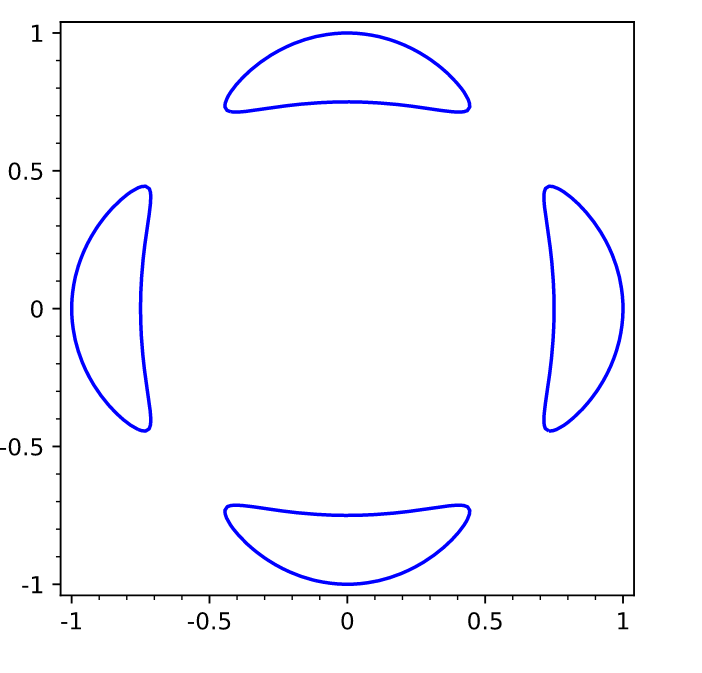
\includegraphics{figures/image_2021-04-09-16-40-49.png}
\caption{image\_2021-04-09-16-40-49}
\end{figure}

\end{remark}

\begin{example}[?]

Consider \(S \coloneqq{\mathbb{P}}^1 \times{\mathbb{P}}^1\), which is
homeomorphic to \(S^2 \times S^2\). The homology is given by
\({\mathbb{Z}}\) in degrees 0 and 4, \({\mathbb{Z}}^{\oplus 2}\) in
degree 3, and 0 elsewhere. What is the intersection form on
\({\mathbb{Z}}^{\oplus 2} = H^2({\mathbb{P}}^1 \times{\mathbb{P}}^1; {\mathbb{Z}})\)?
The two generators are
\(f_1 = [S^2 \times{\operatorname{pt}}], f_2 = [ {\operatorname{pt}}\times S^2]\).
We can compute

\begin{itemize}
\tightlist
\item
  \(f_1 \cdot f_1 = 0\)
\item
  \(f_1 \cdot f_2 = 1\)
\item
  \(f_2 \cdot f_2 = 0\)
\end{itemize}

This is because we can perturb these to be transverse:

\begin{figure}
\centering
\resizebox{\columnwidth}{!}{%
\begin{tikzpicture}
\fontsize{44pt}{1em} 
\node (node_one) at (0,0) { \import{/home/zack/SparkleShare/github.com/Notes/Class_Notes/2021/Spring/FourManifolds/sections/figures}{2021-04-07_14-39.pdf_tex} };
\end{tikzpicture}
}
\end{figure}

Since \(f_2 \cap f_2 ' = \emptyset\), we have
\(f_2 \cdot f_2' = f_2 \cdot f_2 = 0\), and similarly with 1. So the
Gram matrix is
\begin{align*}
G = 
\begin{bmatrix}
0 & 1 
\\
1 & 0
\end{bmatrix}
.\end{align*}

So setting \(C = {\mathbb{P}}^1 \times{\mathbb{P}}^1 = V(f_{2, 3})\), a
function of bidegree \((2, 3)\), writing the coordinates as
\([x: y], [z: w]\), we can write this as
\(x^2 z^3 + y^2 z^2 w + xy w^3 = 0\). We get
\begin{align*}
2g(C) - 2 = (K_{{\mathbb{P}}^1 \times{\mathbb{P}}^1} + 2f_1 + 3f_2) \cdot (2f_1 + 3f_2) = f_2 \cdot (2f_1 + 3f_2) = 2
,\end{align*}
since \(K_{{\mathbb{P}}^1} \circ = -2f_1 - 2f_2\) and so \(g(C) = 2\).

\end{example}

\hypertarget{friday-april-09}{%
\section{Friday, April 09}\label{friday-april-09}}

\begin{remark}

Recall the adjunction formula: for
\(D \subset X \in {\mathsf{Mfd}}_{\mathbb{C}}\) a codimension 1 complex
submanifold, we have
\begin{align*}
K_D = (K_x + {\mathcal{O}}_x(0)) { \left.{{}} \right|_{{D}} }
.\end{align*}
We'll apply this to curves \(C\) in a surface \(S\). Recall the genus
formula, which was given by \(2g(C) - 2= (C+ K_S)\cdot C\). For example,
a degree 4 equation in \({\mathbb{P}}^2\) carves out a genus
\(g(C) = 3\) complex curve.

\end{remark}

\begin{remark}

Recall that line bundles on \({\mathbb{CP}}^n\) were in bijection with
\({\mathbb{Z}}\), where send \(d\) to a bundle
\({\mathcal{O}}(d) \coloneqq{\mathcal{O}}_{{\mathbb{CP}}^N}(d)\). We
produced the tautological line bundle \({\mathcal{O}}(-1)\) whose fiber
over \(\mathbf{x} \subseteq {\mathbb{CP}}^n\) is the line in
\({\mathbb{C}}^n\) spanned by its coordinates. We have
\({\mathcal{O}}(-1)^\vee\coloneqq{\mathcal{O}}(1)\), and
\({\mathcal{O}}(n)\coloneqq{\mathcal{O}}(1)^{\otimes n}\).
Alternatively, it was characterized in terms of homogeneous functions,
where the fiber \({\mathcal{O}}(n)_{\mathbf{x}}\) are the linear
functions \(L\) on lines
\(\left\{{\lambda \mathbf{x}}\right\} \to {\mathbb{C}}\) such that
\(L(\lambda p) = \lambda^n L(p)\). Noting that these are linear
functions, such \(L\) form a 1-dimensional
\({\mathbb{C}}{\hbox{-}}\)vector space.

\end{remark}

\begin{example}[K3 Surfaces]

The classic example is \(x_0 \in {\mathcal{O}}(1)_{\mathbf{x}}\) since
\(x_0( \lambda p) = \lambda x_0 (p)\). Similarly,
\(x_0^2 + x_1 x_2 \in {\mathcal{O}}(2)_{\mathbf{x}}\) since
\begin{align*}
x_0^2 + x_1 x_2 (\lambda p) = \lambda^2 (x_0^2 + x_1 x_2(p))
.\end{align*}

\end{example}

\begin{remark}

Note that the global sections were given by
\(\Gamma^0({\mathbb{P}}^n, {\mathcal{O}}(d)) = H^0({\mathbb{P}}^n; {\mathcal{O}}(d))\)
was the span of degree \(d\) monomials in \(x_0, \cdots, x_n\). For
example \(x_0^2 + x_1 x_2\) is a well-defined element of
\({\mathcal{O}}(2)_p\) which varies holomorphically with \(p\), yielding
a section:

\begin{figure}
\centering
\resizebox{\columnwidth}{!}{%
\begin{tikzpicture}
\fontsize{43pt}{1em} 
\node (node_one) at (0,0) { \import{/home/zack/SparkleShare/github.com/Notes/Class_Notes/2021/Spring/FourManifolds/sections/figures}{2021-04-09_14-11.pdf_tex} };
\end{tikzpicture}
}
\end{figure}

\end{remark}

\begin{example}[?]

For a K3 surface, consider
\(S = \left\{{ \sum_{i=0}^4 x_i^4 = 0 }\right\} \subset {\mathbb{CP}}^3\).
By the adjunction formula,
\begin{align*}
K_S = { \left.{{\qty{ K_{{\mathbb{CP}}^3} \otimes{\mathcal{O}}_{{\mathbb{CP}}^3}(S) }}} \right|_{{S}} }
.\end{align*}
Note that if \(s\in H^0(\mathcal{L})\), we can recover
\({\mathcal{O}}(\operatorname{Div}S) = \mathcal{L}\). Moreover,
\(K_{{\mathbb{CP}}^3} = {\mathcal{O}}(-4)\) and
\({\mathcal{O}}_{{\mathbb{CP}}^3}(S) = {\mathcal{O}}(4)\) since we can
view the formula as a function on the tautological line, which yields a
section. So we get
\(K_S = {\mathcal{O}}(-4) \otimes{\mathcal{O}}(4) = {\mathcal{O}}(0) = {\mathcal{O}}\),
i.e.~these yield actual functions on \({\mathbb{CP}}^n\) since they're
products of functions that scale by \(\lambda^{-4}\) and functions that
scale by \(\lambda^4\). We're using the fact that
\({\mathcal{O}}_{\mathbf{p} = [x_0: \cdots : x_n]}\) are functions \(L\)
such that \(L(\lambda p) = \lambda^0 L(p) = L(p)\), which yields a
well-defined function on \({\mathbb{CP}}^n\). So quartics in
\({\mathbb{P}}^3\) have trivial canonical bundle,
i.e.~\(K_S = {\mathcal{O}}_S\) for
\(S = V(x_0^4 + x_1^4 + x_2^4 + x_3^4)\).

\end{example}

\begin{remark}

We know that \(H^0(S, K_S)\) are the globally holomorphic 2-forms on
\(S\), and here this is isomorphic to
\(H^0(S, {\mathcal{O}}_S) = {\mathbb{C}}\Omega_S\) for some single
holomorphic 2-form. Moreover \(\operatorname{Div}(\Omega_S) = 0\) since
\({\mathcal{O}}( \operatorname{Div}( \Omega_S)) = K_S = {\mathcal{O}}_S\).
So these are the analogs of elliptic curves in dimension 2, since for
example \(E \coloneqq{\mathbb{C}}/ \Lambda\) has a nonvanishing section
\(\,dz\in H^0(E, K_E)\), and we can write \(E = V(f)\) for \(f\) a cubic
in \({\mathbb{P}}^3\), and we computed the genus of cubics. Moreover,
every genus 1 curve is \({\mathbb{C}}\) mod a lattice.

\end{remark}

\begin{remark}

Recall an exercise from the notes: computing the Hodge diamond of a
genus 5 curve. We'll compute the diamond for a K3 surface:

\begin{center}
\begin{tikzcd}
    && {h^{2, 2}} \\
    & {h^{3, 1}} && {h^{1, 3}} \\
    {h^{2, 0}} && {h^{1, 1}} && {h^{0, 2}} \\
    & {h^{1, 0}} && {h^{0, 1}} \\
    && {h^{0, 0}}
\end{tikzcd}
\end{center}

\begin{quote}
\href{https://q.uiver.app/?q=WzAsOSxbMiwwLCJoXnsyLCAyfSJdLFsxLDEsImheezMsIDF9Il0sWzMsMSwiaF57MSwgM30iXSxbMCwyLCJoXnsyLCAwfSJdLFsyLDIsImheezEsIDF9Il0sWzQsMiwiaF57MCwgMn0iXSxbMSwzLCJoXnsxLCAwfSJdLFszLDMsImheezAsIDF9Il0sWzIsNCwiaF57MCwgMH0iXV0=}{Link
to Diagram}
\end{quote}

We know \(h^{2, 0} = H^0( S, \Omega_S^2)\), which yields 1s:

\begin{center}
\begin{tikzcd}
    && 1 \\
    & {h^{3, 1}} && {h^{1, 3}} \\
    1 && {h^{1, 1}} && 1 \\
    & {h^{1, 0}} && {h^{0, 1}} \\
    && 1
\end{tikzcd}
\end{center}

\begin{quote}
\href{https://q.uiver.app/?q=WzAsOSxbMiwwLCIxIl0sWzEsMSwiaF57MywgMX0iXSxbMywxLCJoXnsxLCAzfSJdLFswLDIsIjEiXSxbMiwyLCJoXnsxLCAxfSJdLFs0LDIsIjEiXSxbMSwzLCJoXnsxLCAwfSJdLFszLDMsImheezAsIDF9Il0sWzIsNCwiMSJdXQ==}{Link
to Diagram}
\end{quote}

We'll use the following theorem:

\begin{theorem}[Lefschetz Hyperplane Theorem]

Let \(X \subset {\mathbb{P}}^n\) with \(\dim X > 3\). Then
\(\pi_1(X) \cong \pi_1(X \cap H)\) for \(H\) a hypersurface intersection
\(X\) at a smooth codimension 1 complex manifold.

\end{theorem}

\begin{remark}

Applying this to \(X = {\mathbb{P}}^3\), we have
\(V(x_0^4 + \cdots + x_3^4) = S\), we have
\(\pi_1({\mathbb{P}}^3) = \pi_1(S)\). We can write
\({\mathbb{P}}^3 = {\mathbb{C}}\cup{\mathbb{C}}^2 \cup{\mathbb{C}}^4\),
which is a cell decomposition with cells only in degrees 0,2,4, and so
in fact \(\pi_1({\mathbb{P}}^n) = 0\).

\end{remark}

\begin{corollary}[?]

K3 surfaces are simply connected, and \(h^1(S; {\mathbb{C}}) = 0\).

\end{corollary}

Note that anything embedded in projective space as a complex submanifold
is Kähler by restricting the Fubini-Study form. Using simple
connectedness and Serre duality, we have

\begin{center}
\begin{tikzcd}
    && 1 \\
    & 0 && 0 \\
    1 && {h^{1, 1}} && 1 \\
    & 0 && 0 \\
    && 1
\end{tikzcd}
\end{center}

\begin{quote}
\href{https://q.uiver.app/?q=WzAsOSxbMiwwLCIxIl0sWzEsMSwiMCJdLFszLDEsIjAiXSxbMCwyLCIxIl0sWzIsMiwiaF57MSwgMX0iXSxbNCwyLCIxIl0sWzEsMywiMCJdLFszLDMsIjAiXSxbMiw0LCIxIl1d}{Link
to Diagram}
\end{quote}

We know \(\chi({\mathcal{O}}_S) = (1/12)(K^2+\chi_{\mathsf{Top}})\), and
since \(K_S = {\mathcal{O}}_S\) is trivial, we have
\(c_1({\mathcal{O}}_S) = 0\). Noting that \(h^{p, q} = H^( \Omega^p)\),
so we can sum the lower-right part of the diamond to get
\(\chi({\mathcal{O}}_S) = 1 - 0 + 1 = 2\), since we take \(p=0\) to get
\(\Omega^p = {\mathcal{O}}\). Computing \(\chi_{\mathsf{Top}}\), we get
\(h_{1, 1} = 20\).

\end{remark}

\hypertarget{monday-april-12}{%
\section{Monday, April 12}\label{monday-april-12}}

\begin{remark}

Last time: the Lefschetz hyperplane theorem. Intersecting a projective
variety of dimension \(d\geq 3\) with a hypersurface \(S\), the map
\(\pi_1({\mathbb{P}}^3) \to \pi_1(S)\) is an isomorphism. We saw that K3
surfaces were thus simply connected, and \(h^1(S; {\mathbb{C}}) = 0\),
so we could compute the Hodge diamond.

\end{remark}

\begin{example}[?]

What is the Hodge diamond for a cubic surface
\(S \subseteq {\mathbb{P}}^3\), such as \(\sum x_i^3 = 0\)? We first
need to compute the canonical bundle \(K\), for which we have a useful
tool: the adjunction formula. This say
\(K_S = \qty{K_{{\mathbb{P}}^3} \otimes{\mathbb{P}}_{{\mathbb{P}}^3}(S) } { \left.{{}} \right|_{{S}} } = \qty{ {\mathcal{O}}(-4) \otimes{\mathcal{O}}(3) }{ \left.{{}} \right|_{{S}} } = { \left.{{ {\mathcal{O}}(-1)}} \right|_{{S}} }\).

\begin{proposition}[?]

Let \(\mathcal{L} \to X\) be a holomorphic line bundle. If
\(h^0( \mathcal{L} ^{-1}) > 0\), then either
\(\mathcal{L} = {\mathcal{O}}\) or \(h^0(\mathcal{L}) = 0\).

\end{proposition}

\begin{slogan}

If a line bundle has a section, its inverse does not.

\end{slogan}

\begin{proof}[?]

Suppose that both \(\mathcal{L}, \mathcal{L}^{-1}\) have a section, so
\(h^0(\mathcal{L}), h^0( \mathcal{L} ) > 0\). Let \(s, t\) be sections
of each, then
\(st\in H^0( \mathcal{L} \otimes\mathcal{L}^{-1}) = H^0({\mathcal{O}}) = {\mathbb{C}}\).
So taking zero loci yields
\(\operatorname{Div}(s) + \operatorname{Div}(t) = 0\) Writing these as
\(\operatorname{Div}(s) \coloneqq\sum n_D D, \operatorname{Div}(t) \coloneqq\sum n_C C\),
we have \(n_D, n_C \geq 0\), which implies that
\(\operatorname{Div}(s) = \operatorname{Div}(t) = 0\). So \(s, t\) are
nowhere vanishing, making
\({\mathcal{O}}\xrightarrow{\cdot s} \mathcal{L}\) is an isomorphism.

\end{proof}

\begin{corollary}[?]

For \(S\) a cubic surface, \(H^0(S; K_S) = 0\).

\end{corollary}

\begin{proof}[?]

This follows because \(K_S = {\mathcal{O}}_S(-1)\), so
\(K_S^{-1}= {\mathcal{O}}_S(1)\) which has a nontrivial section: namely
\({\mathcal{O}}_{{\mathbb{CP}}^1}(1)\) which has sections vanishing
along hyperplanes.

\begin{figure}
\centering
\resizebox{\columnwidth}{!}{%
\begin{tikzpicture}
\fontsize{43pt}{1em} 
\node (node_one) at (0,0) { \import{/home/zack/SparkleShare/github.com/Notes/Class_Notes/2021/Spring/FourManifolds/sections/figures}{2021-04-12_14-06.pdf_tex} };
\end{tikzpicture}
}
\end{figure}

Letting \(H\) be a hyperplane containing \(S\), there exists an
\(f\in H^0({\mathbb{P}}^3; {\mathcal{O}}_{{\mathbb{CP}}^3}(1))\). Since
\(\operatorname{Div}(f) = H\), the restriction
\({ \left.{{f}} \right|_{{S}} }\) is a section of
\({\mathcal{O}}_S(-1) = K_S^{-1}\) which is not identically zero and
vanishes along \(H \cap S\).

\end{proof}

We now know \(h^0(S; K_S) = 0\), and this equals
\(h^0(S, \Omega^2) = h^{2, 0}(S)\), so we have the following Hodge
diamond:

\begin{center}
\begin{tikzcd}
    && 1 \\
    & 0 && 0 \\
    0 && {h^{1, 1}} && 0 \\
    & 0 && 0 \\
    && 1
\end{tikzcd}
\end{center}

\begin{quote}
\href{https://q.uiver.app/?q=WzAsOSxbMiwwLCIxIl0sWzEsMSwiMCJdLFszLDEsIjAiXSxbMCwyLCIwIl0sWzIsMiwiaF57MSwgMX0iXSxbNCwyLCIwIl0sWzEsMywiMCJdLFszLDMsIjAiXSxbMiw0LCIxIl1d}{Link
to Diagram}
\end{quote}

We have \(h^{0, 1} + h^{1, 0} = h^1 = 0\) since \(S\) is simply
connected. We can now apply Noether's formula as before:
\(\chi({\mathcal{O}}_S) = {1\over 12} (K_S^2 + \chi_{\mathsf{Top}}(S))\).
We have \(K_S = {\mathcal{O}}_S(-1)\), so
\(K_S^2 = c_1( {\mathcal{O}}(-1))^2\), and
\(\chi({\mathcal{O}}_S) = 1-0+1 = 1\). We now want to compute
\(\int_S \qty{- c_1({\mathcal{O}}_S(1)) }^2\). We know
\(c_1(\mathcal{L}) = [ \operatorname{Div}s]\) where
\(s\in H^0( \mathcal{L} )\) is a section of a line bundle. This equals
\([H \cap S]\). On the other hand,
\(\int_S c_1 \qty{ {\mathcal{O}}_S(1)}^2\) is the self-intersection
number of \(H \cap S\).

\hfill\break

Take \(H_1 \coloneqq\left\{{ x_0 = 0 }\right\}\) and
\(H_2 \coloneqq\left\{{ x_1 = 0 }\right\}\). Points in this intersection
are of the form \([0:0:1:\zeta_6^a]\) where \(a=1,3,5\) since this is in
the triple intersection \(H_1 \cap H_2 \cap S\). So there are exactly 3
points here, and in fact \(\deg S =3\). This is the same as integrating
\(\int_{{\mathbb{P}}^3} c_1(S) c_1( {\mathcal{O}}(1)) c_1( {\mathcal{O}}(2))\),
which contains 3 elements in \(H^2\) and lands in \(H^6\), so this
yields a number.

\hfill\break

We thus have
\(K_S = {\mathcal{O}}_S(-1) \coloneqq{\mathcal{O}}_{{\mathbb{CP}}^3}(-1) { \left.{{}} \right|_{{S}} }\).
Thus \(\chi_{\mathsf{Top}}(S) = 9\) and \(h^{1, 1} = 7\).

\end{example}

\begin{example}[Hypersurfaces]

Note that a degree 5 surface (a quintic) such as \(x_0^5 + x_3^5 = 0\)
would be harder, since \(h^{2, 0} \neq 0\). We would get
\(K_S = {\mathcal{O}}(-4) \otimes{\mathcal{O}}(5) { \left.{{}} \right|_{{S}} } = {\mathcal{O}}_S(1)\),
and there are nontrivial sections so
\(h^0(K_S) = {\operatorname{span}}{x_0, x_1, x_2, x_3}\). This follows
because there is a map given by restriction which turns out to be an
isomorphism
\begin{align*}
0 \to H^0({\mathbb{P}}^3; {\mathcal{O}}(1)) & \xrightarrow{\mathop{\mathrm{res}}_S} H^0(S; {\mathcal{O}}(1)) \to 0 \\
f &\mapsto { \left.{{f}} \right|_{{S}} }
.\end{align*}

Injectivity isn't difficult, surjectivity is harder. We have a SES
\begin{align*}
0 \to {\mathcal{O}}_{{\mathbb{CP}}^3}(-S) \to {\mathcal{O}}_{{\mathbb{CP}}^3} \to {\mathcal{O}}_S \to 0
.\end{align*}
Tensor all of these with \({\mathcal{O}}(1)\) to obtain
\begin{align*}
0 \to {\mathcal{O}}_{\mathbb{CP}}^3(-4) \to {\mathcal{O}}_{{\mathbb{CP}}^3}(1) \to {\mathcal{O}}_S(1) \to 0
.\end{align*}
Taking the associated LES yields

\begin{center}
\begin{tikzcd}
    {H^1({\mathcal{O}}_{{\mathbb{CP}}^3}(-4)) =_? 0} \\
    \\
    {H^0({\mathcal{O}}_{{\mathbb{CP}}^3}(-4)) = 0} && \textcolor{rgb,255:red,92;green,92;blue,214}{H^0({\mathcal{O}}_{{\mathbb{CP}}^3}(-1)) = {\mathbb{C}}\left\langle{x_0, x_1, x_2, x_3}\right\rangle} && \textcolor{rgb,255:red,92;green,92;blue,214}{H^0({\mathcal{O}}_{S}(1))} \\
    0
    \arrow[from=4-1, to=3-1]
    \arrow[from=3-1, to=3-3]
    \arrow[color={rgb,255:red,92;green,92;blue,214}, from=3-3, to=3-5]
    \arrow[from=3-5, to=1-1, out=0, in=180]
\end{tikzcd}
\end{center}

\begin{quote}
\href{https://q.uiver.app/?q=WzAsNSxbMCwyLCJIXjAoXFxPT197XFxDUF4zfSgtNCkpID0gMCJdLFsyLDIsIkheMChcXE9PX3tcXENQXjN9KC0xKSkgPSBcXENDIFxcZ2Vuc3t4XzAsIHhfMSwgeF8yLCB4XzN9IixbMjQwLDYwLDYwLDFdXSxbNCwyLCJIXjAoXFxPT197U30oMSkpIixbMjQwLDYwLDYwLDFdXSxbMCwwLCJIXjEoXFxPT197XFxDUF4zfSgtNCkpID1fPyAwIl0sWzAsMywiMCJdLFs0LDBdLFswLDFdLFsxLDIsIiIsMCx7ImNvbG91ciI6WzI0MCw2MCw2MF19XSxbMiwzXV0=}{Link
to Diagram}
\end{quote}

This gives us a way to relate things back to the cohomology of
\({\mathbb{CP}}^3\). Showing that the indicated term is zero involves
computing Čech cohomology.

It turns out that \(h^0(K_S) = 4\) here, and it turns out that the Hodge
diamond is the following:

\begin{center}
\begin{tikzcd}
    && 1 \\
    & 0 && 0 \\
    4 && {h^{1, 1} = 45} && 4 \\
    & 0 && 0 \\
    && 1
\end{tikzcd}
\end{center}

\begin{quote}
\href{https://q.uiver.app/?q=WzAsOSxbMiwwLCIxIl0sWzEsMSwiMCJdLFszLDEsIjAiXSxbMCwyLCI0Il0sWzQsMiwiNCJdLFsxLDMsIjAiXSxbMywzLCIwIl0sWzIsNCwiMSJdLFsyLDIsImheezEsIDF9ID0gNDUiXV0=}{Link
to Diagram}
\end{quote}

Here \(K_S^2 = c_1({\mathcal{O}}_S(1))^2 = 5\) and
\(\chi_{\mathsf{Top}}= 55\).

\end{example}

\begin{example}[Products]

Consider now a product of curves \(C \times D\) of genera \(g, h\)
respectively. Computing the Hodge diamond is easy here due to the
Kunneth formula:
\begin{align*}
H^k(S; {\mathbb{C}}) = \bigoplus_{i+j = k} H^i(C; {\mathbb{C}}) \otimes H^j(D; {\mathbb{C}})
.\end{align*}

What is the actual map? Take cohomology classes \([\alpha], [\beta]\),
closed \(i\) and \(j\) forms respectively. The surface has two maps:

\begin{center}
\begin{tikzcd}
    S && C \\
    \\
    D
    \arrow["{\pi_C}", from=1-1, to=1-3]
    \arrow["{\pi_D}"', from=1-1, to=3-1]
\end{tikzcd}
\end{center}

Here we send
\([\alpha] \otimes[ \beta] \mapsto [ \pi_C^* \alpha\wedge \pi_D^* \beta]\)
where we take pullbacks. Note that \(\pi_D, \pi_C\) are holomorphic
maps, and pullbacks of \((p, q)\) forms are still \((p, q)\) forms. Thus
the Kunneth formula gives a decomposition
\begin{align*}
H^{p, q}(S; {\mathbb{C}}) 
= \sum_{\substack{ i_1 + j_1 = p \\ i_2 + j_2 = q }} H^{i_1, j_1}(C) \oplus H^{i_2, j_2}(D)
.\end{align*}
So we can ``tensor'' the Hodge diamonds:

\begin{center}
\begin{tikzcd}
    & 1 &&&& 1 \\
    g && g && h && h \\
    & 1 &&&& 1 \\
    \\
    &&& 1 \\
    && {g+h} && {g+h} \\
    & gh && {2 + 2gh} && gh \\
    && {g+h} && {g+h} \\
    &&& 1
\end{tikzcd}
\end{center}

\begin{quote}
\href{https://q.uiver.app/?q=WzAsMTcsWzEsMCwiMSJdLFswLDEsImciXSxbMiwxLCJnIl0sWzEsMiwiMSJdLFs1LDAsIjEiXSxbNCwxLCJoIl0sWzYsMSwiaCJdLFs1LDIsIjEiXSxbMyw0LCIxIl0sWzIsNSwiZytoIl0sWzQsNSwiZytoIl0sWzIsNywiZytoIl0sWzQsNywiZytoIl0sWzEsNiwiZ2giXSxbNSw2LCJnaCJdLFszLDgsIjEiXSxbMyw2LCIyICsgMmdoIl1d}{Link
to Diagram}
\end{quote}

\end{example}

\begin{remark}

Check out complete intersections.

\end{remark}

\hypertarget{blowups-and-blowdowns-wednesday-april-14}{%
\section{Blowups and Blowdowns (Wednesday, April
14)}\label{blowups-and-blowdowns-wednesday-april-14}}

\begin{definition}[Blowup]

Let \(S \in {\mathsf{Mfd}}_{\mathbb{C}}^2\) be a complex surface and
\(p\in S\) a point, and let \((x, y)\) be local holomorphic coordinates
on a neighborhood of \(U\) containing \(p\). Without loss of generality,
\(p = (0, 0)\) in these coordinates. Set
\(U^* \coloneqq U \setminus\left\{{p}\right\}\), and consider the
holomorphic map
\begin{align*}
\phi: U^* &\to U \times{\mathbb{CP}}^2 \\
(x, y) & \mapsto ( (x, y), [x: y] )
.\end{align*}
We'll define the \textbf{blowup at \(p\)} to be
\(\mathop{\mathrm{Bl}}_p(U) { \operatorname{cl}} (\phi(U^*))\) to be the
closure of the image of \(U^*\).

\end{definition}

\begin{observation}

There is a map \(\mathop{\mathrm{Bl}}_p(U) \to U\) given by projection
onto the first coordinate which is the identity on \(U^*\).

\begin{figure}
\centering
\resizebox{\columnwidth}{!}{%
\begin{tikzpicture}
\fontsize{45pt}{1em} 
\node (node_one) at (0,0) { \import{/home/zack/SparkleShare/github.com/Notes/Class_Notes/2021/Spring/FourManifolds/sections/figures}{2021-04-14_13-56.pdf_tex} };
\end{tikzpicture}
}
\end{figure}

Here \(q\) maps to the pair \((q, s)\) where \(s\) is the slope of a
line through \(q\), and this will be continuous.

\todo[inline]{? Missed part}

We claim that
\(\pi_U^{-1}(0, 0) \subset \mathop{\mathrm{Bl}}_p(U) = \left\{{ p }\right\} \times{\mathbb{CP}}^1\),
and for a fixed \(9x_0, y_0) \in U^*\), considering
\(\phi(x_0 t, y_0 t)\) as \(t\to 0\), we can write
\begin{align*}
( (x_0 t, y_0 t), [x_0: y_0] ) \in U \times{\mathbb{CP}}^1 \\
\overset{t\to 0} ( (0, 0) [x_0: y_0] ) \subset { \operatorname{cl}} (\phi(U^*))
.\end{align*}
So approaching \((0, 0)\) along any slope \(s\) just yields the point
\((0, s)\) in the blowup.

\end{observation}

\begin{remark}

We can thus write
\begin{align*}
\mathop{\mathrm{Bl}}_pS S \setminus\left\{{p}\right\} {\coprod}_{U^*} \mathop{\mathrm{Bl}}_p U
.\end{align*}

Writing \(\pi: \mathop{\mathrm{Bl}}_pS\to S\), we have
\(\pi^{-1}(p) \cong {\mathbb{CP}}^1\) and \(\pi^{-1}(q)\) is a point for
all \(q\neq p\). Then all limits approaching \(p\) in \(S\) turn into
distinct limit points in \(\mathop{\mathrm{Bl}}_p(S)\)

\begin{figure}
\centering
\resizebox{\columnwidth}{!}{%
\begin{tikzpicture}
\fontsize{45pt}{1em} 
\node (node_one) at (0,0) { \import{/home/zack/SparkleShare/github.com/Notes/Class_Notes/2021/Spring/FourManifolds/sections/figures}{2021-04-14_14-06.pdf_tex} };
\end{tikzpicture}
}
\end{figure}

\end{remark}

\begin{slogan}

The blowup separates all tangent directions at \(p\).

\end{slogan}

\begin{example}[?]

Consider
\begin{align*}
\left\{{ y^2 = x^3 - x^2 }\right\} \subseteq {\mathbb{C}}^2
.\end{align*}

This yields a nodal curve with a double-point:

\begin{figure}
\centering
\resizebox{\columnwidth}{!}{%
\begin{tikzpicture}
\fontsize{45pt}{1em} 
\node (node_one) at (0,0) { \import{/home/zack/SparkleShare/github.com/Notes/Class_Notes/2021/Spring/FourManifolds/sections/figures}{2021-04-14_14-11.pdf_tex} };
\end{tikzpicture}
}
\end{figure}

Here we'll consider \(\mathop{\mathrm{Bl}}_{(0, 0)} {\mathbb{C}}^2\).

\begin{definition}[Strict Transform]

Letting \(C \subset S\) be a curve, define the \textbf{strict transform}
\begin{align*}
\widehat{C} \coloneqq{ \operatorname{cl}} ( \pi^{-1}(C \setminus\left\{{p}\right\} ) )
.\end{align*}

\end{definition}

Note that approaching by different sequences yields different limiting
slopes

\begin{figure}
\centering
\resizebox{\columnwidth}{!}{%
\begin{tikzpicture}
\fontsize{45pt}{1em} 
\node (node_one) at (0,0) { \import{/home/zack/SparkleShare/github.com/Notes/Class_Notes/2021/Spring/FourManifolds/sections/figures}{2021-04-14_14-15.pdf_tex} };
\end{tikzpicture}
}
\end{figure}

The curve in the blowup is called the \textbf{exceptional divisor}.

\end{example}

\begin{example}[?]

Consider all lines in \({\mathbb{CP}}^2\) through \([0:0:1]\), which we
can model in the following way:

\begin{figure}
\centering
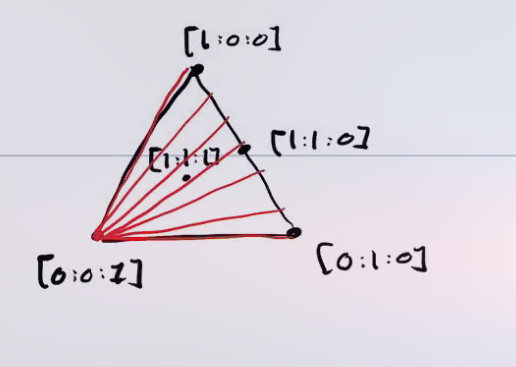
\includegraphics{figures/image_2021-04-14-14-18-15.png}
\caption{image\_2021-04-14-14-18-15}
\end{figure}

These are in bijection with \({\mathbb{CP}}^1\) since there is always a
unique line through \([0:0:1]\) and \([s:t:0]\), where the latter is a
copy of \({\mathbb{CP}}^1\) as \(s,t\) are allowed to vary. So consider
\(\mathop{\mathrm{Bl}}_{p}{\mathbb{CP}}^2\) for \(p=[0:0:1]\), and
consider the strict transforms of the lines \(L\) to obtain
\(\widehat{L} \subset \mathop{\mathrm{Bl}}_p {\mathbb{CP}}^2\). Any two
are disjoint since they pass through different slopes of the exceptional
divisor. Thus the red lines in the blowup go through distinct slopes,
yielding a fibration of \({\mathbb{CP}}^1\)s:

\begin{figure}
\centering
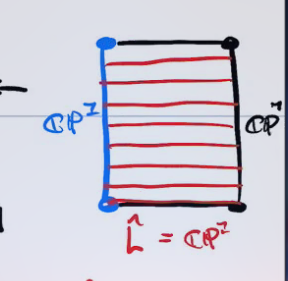
\includegraphics{figures/image_2021-04-14-14-24-31.png}
\caption{image\_2021-04-14-14-24-31}
\end{figure}

So consider the map
\begin{align*}
\sigma: \mathop{\mathrm{Bl}}_p {\mathbb{CP}}^2 &\to {\mathbb{CP}}^2 \\
p \in \widehat{L} &\mapsto [0:s:t]
.\end{align*}

which projects points to the boundary copy of \({\mathbb{CP}}^1\):

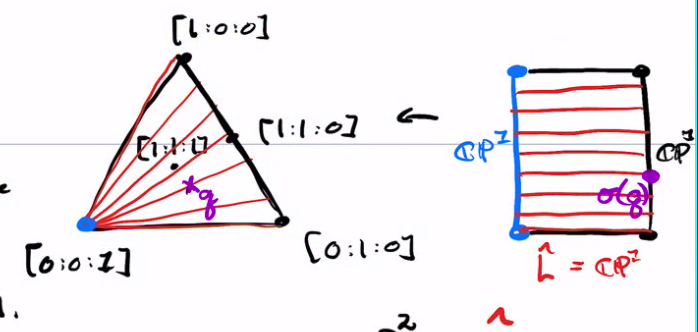
\includegraphics{figures/image_2021-04-14-14-25-44.png}

We can't necessarily project from the blue point itself, but if we add
in the data of a tangent vector at that point, the map becomes
well-defined. Thus the blowup makes projecting from a point in
\({\mathbb{CP}}^2\) to a line in \({\mathbb{CP}}^2\) a well-defined map
on \(\mathop{\mathrm{Bl}}{\mathbb{CP}}^2\).

\end{example}

\begin{remark}

This is referred to as \({\mathbb{F}}_1\), the \textbf{first Hirzebruch
surface}.

\end{remark}

\begin{proposition}[?]

For \(S\in {\mathsf{Mfd}}_{\mathbb{R}}(C^\infty)\) a smooth manifold, we
can identify
\begin{align*}
\mathop{\mathrm{Bl}}_p S = S \mathop{ \Large\scalebox{0.8}{\raisebox{0.4ex}{\#}}}\mkern 1.5mu\overline{\mkern-1.5mu{\mathbb{CP}}^2\mkern-1.5mu}\mkern 1.5mu
.\end{align*}

\end{proposition}

\begin{proof}[?]

It suffices to work in coordinate charts and prove this for \(p=0\).

\begin{claim}

\begin{align*}
\mathop{\mathrm{Bl}}_0 {\mathbb{C}}^2 = \mathop{\mathrm{Tot}}( {\mathcal{O}}_{{\mathbb{CP}}^1}(-1) )
.\end{align*}

\end{claim}

Recall that this was the tautological line bundle that whose fibers at a
point \(p\in {\mathbb{CP}}^1\) was the line in \({\mathbb{C}}^2\)
spanned by \(p\). We can write this as
\(\left\{{ [x:y] {~\mathrel{\Big|}~}(x, y) \in L_{[x:y]} }\right\}\):

\begin{figure}
\centering
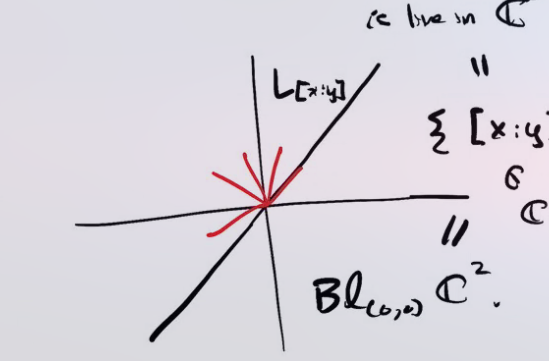
\includegraphics{figures/image_2021-04-14-14-32-58.png}
\caption{image\_2021-04-14-14-32-58}
\end{figure}

We have
\({\mathcal{O}}(-1) \xrightarrow{\sim} \mkern 1.5mu\overline{\mkern-1.5mu{\mathcal{O}}(1)\mkern-1.5mu}\mkern 1.5mu\),
where this map is a diffeomorphism that can be constructed using a
Hermitian metric. However we can identify \({\mathcal{O}}(1)\) with the
set of lines in \({\mathbb{CP}}^2\) through \([0:0:1]\), leaving out the
point \([0:0:1]\) itself. This follows by checking that there exists a
section that vanishes at only one point. In fact
\(\mathop{\mathrm{Tot}}{\mathcal{O}}(1)\) is diffeomorphic to the
complement of a ball in \({\mathbb{CP}}^2\), which ends up precisely
being taking a connect-sum. So we obtain
\(\mathop{\mathrm{Bl}}_{0} {\mathbb{C}}^2 \cong {\mathbb{C}}^2 \mathop{ \Large\scalebox{0.8}{\raisebox{0.4ex}{\#}}}\mkern 1.5mu\overline{\mkern-1.5mu{\mathbb{CP}}^2\mkern-1.5mu}\mkern 1.5mu\).

\end{proof}

\begin{proof}[Alternative]

Cut out a ball \(B^4 \subseteq {\mathbb{C}}^2\), so
\({{\partial}}B^4 = S^3 = \left\{{ {\left\lvert {x} \right\rvert}^2 + {\left\lvert {y} \right\rvert}^2 = \varepsilon}\right\}\).
Then \(\mathop{\mathrm{Bl}}_0 {\mathbb{C}}^2\) is the result of
collapsing \(S^3\) along an \(S^1{\hbox{-}}\)foliation
\((e^{i\theta} x, e^{i\theta}y)\). This has an \(S^2\) quotient,
yielding the Hopf fibration
\begin{align*}
S^1 \hookrightarrow S^3 \to S^2
.\end{align*}

\end{proof}

\begin{exercise}[?]

Show that the blowup over \({\mathbb{R}}\) is gluing in a mobius strip.

\end{exercise}

See the Tate curve!

\hypertarget{friday-april-16}{%
\section{Friday, April 16}\label{friday-april-16}}

\begin{remark}

Last time: we defined the blowup
\(\mathop{\mathrm{Bl}}_0{\mathbb{C}}^2\) as the closure of
\begin{align*} 
\mathop{\mathrm{Bl}}_0 {\mathbb{C}}^2 \coloneqq{ \operatorname{cl}} 
\left\{{ (x, y), [x:y] {~\mathrel{\Big|}~}(x, y) \neq 0 }\right\} \subseteq {\mathbb{C}}^2 \times{\mathbb{CP}}^2 
.\end{align*}
This had the effect of adding in all limits of slopes as points approach
\((0, 0) \in {\mathbb{C}}^2\). We defined this using local holomorphic
coordinate charts to \({\mathbb{C}}^2\). Why is this a complex manifold?
We can cover it with charts: given a point \((x, \mu)\) where
\(\mu = {y \over x}\in {\mathbb{P}}^1\) is a slope, we can form a first
chart by sending
\begin{align*}
(x, \mu) \mapsto \left\{{ (x, x\mu), [1: \mu] }\right\}
.\end{align*}
This yields the first chart, as long as the slope is not infinite, so
this applies to all finite slopes. The second chart will work for all
nonzero slopes, where we take
\begin{align*}
(v, y)\in {\mathbb{C}}^2 \mapsto \left\{{ (yv, y), [v: 1] }\right\}
.\end{align*}
Note that restricting to \((x, y) = (0, 0)\), these give the standard
\({\mathbb{C}}{\hbox{-}}\)charts on \({\mathbb{CP}}^2\). How do these
two charts glue? When \(\mu, \nu \neq 0\), we have well-defined
transition functions \(\mu = \nu ^{-1}\) and \(x=y\nu\).

\end{remark}

\begin{remark}

Recall that for a complex curve \(C \in {\mathsf{Mfd}}_{\mathbb{C}}^2\),
we have the blowup morphism \(\pi: \mathop{\mathrm{Bl}}_pS\to S\) and we
defined the \textbf{strict transform}
\(\widehat{C} \coloneqq{ \operatorname{cl}} \pi^{-1}(C\setminus\left\{{{\operatorname{pt}}}\right\})\).

\begin{figure}
\centering
\resizebox{\columnwidth}{!}{%
\begin{tikzpicture}
\fontsize{42pt}{1em} 
\node (node_one) at (0,0) { \import{/home/zack/SparkleShare/github.com/Notes/Class_Notes/2021/Spring/FourManifolds/sections/figures}{2021-04-16_14-02.pdf_tex} };
\end{tikzpicture}
}
\end{figure}

Here \(E={\mathbb{CP}}^1\) is the exceptional curve of the blowup, and
intersects the curve twice. This has the effect of changing \(D\) into
an embedded curve.

\begin{quote}
Note that here \(\pi^* D = \widehat{D} + 2E\), where we'll define this
next.
\end{quote}

\end{remark}

\begin{definition}[Pullback of a Curve]

The \textbf{pullback} of \(C\), denoted \(\pi^* C\), is constructed by
writing \(C = V(f)\) locally. We then set
\(\pi^* C \coloneqq V( \pi^* f)\).

\end{definition}

\begin{example}[?]

Take \(C \coloneqq\left\{{ y=x }\right\} \subset {\mathbb{C}}^2\) and
consider \(\mathop{\mathrm{Bl}}_0 {\mathbb{C}}^2\). Then
\begin{align*}
\widehat{C}  \coloneqq{ \operatorname{cl}} \left\{{ \qty{ (x, x), [x:x]} {~\mathrel{\Big|}~}x\neq 0  }\right\} = { \operatorname{cl}} \left\{{ \qty{ (x, x), [1:1] } {~\mathrel{\Big|}~}x\neq 0 }\right\} \subset \mathop{\mathrm{Bl}}_0 {\mathbb{C}}^2
.\end{align*}
By projecting onto the first component,
\(\pi:\widehat{C} \xrightarrow{\sim} C\) is an isomorphism. We can
compute the pullback: we first have
\(\pi^* C = \pi^* V(y-x) = V( \pi^*(y-x))\), so consider \(\pi^*(y-x)\)
in the coordinate chart \((x, \mu)\). In this chart, \(y=x\mu\), and so
\(\pi^*(y-x) = x\mu - x = x(\mu - 1)\), and so
\begin{align*}
V(\pi^*(y-x)) = V(x) + V(\mu -1) \implies \pi^* C = E + \widehat{C} \text{ as a divisor}
.\end{align*}

\end{example}

\begin{example}[A nodal curve]

Take the nodal curve \(C = \left\{{ y^2 - x^3 + x^2 }\right\}\):

\begin{figure}
\centering
\resizebox{\columnwidth}{!}{%
\begin{tikzpicture}
\fontsize{44pt}{1em} 
\node (node_one) at (0,0) { \import{/home/zack/SparkleShare/github.com/Notes/Class_Notes/2021/Spring/FourManifolds/sections/figures}{2021-04-16_14-15.pdf_tex} };
\end{tikzpicture}
}
\end{figure}

The pullback is then given by
\begin{align*}
\pi^* C 
&= V( \pi^* (y^2 - x^3 + x^2) ) \\
&= V(\mu^2x^2 -x^3 + x^2) \\
&= V(x^2) + V(\mu^2 - x + 1) \\
&= 2V(x) + V(\mu^2 -x + 1)
.\end{align*}

\begin{figure}
\centering
\resizebox{\columnwidth}{!}{%
\begin{tikzpicture}
\fontsize{44pt}{1em} 
\node (node_one) at (0,0) { \import{/home/zack/SparkleShare/github.com/Notes/Class_Notes/2021/Spring/FourManifolds/sections/figures}{2021-04-16_14-17.pdf_tex} };
\end{tikzpicture}
}
\end{figure}

In the second coordinate chart, we have
\begin{align*}
\pi^* C = V(y^2 - y^4 \nu^3 +y^2 \nu^2) = 2V(y) + V(1-y\nu^3 + \nu^2
.\end{align*}

\begin{figure}
\centering
\resizebox{\columnwidth}{!}{%
\begin{tikzpicture}
\fontsize{43pt}{1em} 
\node (node_one) at (0,0) { \import{/home/zack/SparkleShare/github.com/Notes/Class_Notes/2021/Spring/FourManifolds/sections/figures}{2021-04-16_14-21.pdf_tex} };
\end{tikzpicture}
}
\end{figure}

Gluing along \(\mu, \nu \neq 0\) we get the following picture for
\(\pi^* C\):

\begin{figure}
\centering
\resizebox{\columnwidth}{!}{%
\begin{tikzpicture}
\fontsize{45pt}{1em} 
\node (node_one) at (0,0) { \import{/home/zack/SparkleShare/github.com/Notes/Class_Notes/2021/Spring/FourManifolds/sections/figures}{2021-04-16_14-22.pdf_tex} };
\end{tikzpicture}
}
\end{figure}

Writing \(C = \left\{{ x=0 }\right\}\), note that \(\widehat{C}\)
doesn't intersect the first coordinate chart. In the \(\mu, x\)
coordinate chart, for example, we can't get an infinite slop:

\begin{figure}
\centering
\resizebox{\columnwidth}{!}{%
\begin{tikzpicture}
\fontsize{45pt}{1em} 
\node (node_one) at (0,0) { \import{/home/zack/SparkleShare/github.com/Notes/Class_Notes/2021/Spring/FourManifolds/sections/figures}{2021-04-16_14-25.pdf_tex} };
\end{tikzpicture}
}
\end{figure}

\end{example}

\hypertarget{change-in-canonical-bundle-formula}{%
\subsection{Change in Canonical Bundle
Formula}\label{change-in-canonical-bundle-formula}}

\begin{question}

Given \(\Omega^2_S = K_S \to S\) the canonical line bundle, can we
relate \(K_{\mathop{\mathrm{Bl}}_p S}\) to \(K_S\)?

\end{question}

\begin{proposition}[?]

\begin{align*}
K_{\mathop{\mathrm{Bl}}_p S} = \pi^* K_S \otimes{\mathcal{O}}_S(E)
.\end{align*}

\end{proposition}

\begin{proof}[?]

We'll abbreviate \(\widehat{S} \coloneqq\mathop{\mathrm{Bl}}_p(S)\). Let
\(\omega\) be a local section of \(K_S\) near \(p\), and in coordinate
charts \((x, y)\), write \(\omega = dx \wedge dy\). In the first
coordinate chart on the blowup, we can write
\begin{align*}
\pi^* \omega = dx \wedge d(x\mu) = dx \wedge (\mu dx + x d\mu) = x\,dx\wedge d\mu
.\end{align*}
Note that \(V(x) = E\), and that pulling back the canonical bundle
yields something vanishing to order 1 (?). So \(\pi^* K_S\) is
isomorphic to the subsheaf of \(K_{\widehat{S}}\) whose sections vanish
along \(E\), which is isomorphic to
\(K_{\widehat{S}} \otimes{\mathcal{O}}(-E)\), since the latter are the
functions which vanish along \(E\). Tensoring both sides with
\({\mathcal{O}}(E)\) yields
\begin{align*}
K_{\widehat{S}} = \pi^* K_S \otimes{\mathcal{O}}_{\widehat{S}}(E)
\end{align*}
as a line bundle, or in divisor notation
\(K_{\widehat{S}} = \pi^* K_S + E\) where we take the divisor
representing the line bundle instead.

\end{proof}

\begin{remark}

Using \(\pi: \widehat{S}\to S\), we get pullback maps
\begin{align*}
\pi^*: H^2(S; {\mathbb{Z}}) &\to H^2(\widehat{S}; {\mathbb{Z}}) \\
\pi^*: \operatorname{Div}(S) &\to \operatorname{Div}(\widehat{S})
.\end{align*}
These are compatible in the sense that
\begin{align*}
[\pi^* C] = \pi^* [C]
.\end{align*}
. This can be seen by expressing
\({\mathcal{O}}_S(C) \cong {\mathcal{O}}_S(A-b)\) for \(A, B\)
hyperplane section. We can assume \(A, B\) avoid \(p\) in their
projective embeddings, making \([C] = [A] - [B]\) since
\(c_1({\mathcal{O}}_S(c)) = [C]\) is the fundamental class of \(C\). So
it suffices to prove the formula for curves \emph{not} passing through
\(p\), but this is obvious! It follows from the fact that
\(\pi: \widehat{S} \setminus E \xrightarrow{\sim} S\setminus\left\{{p}\right\}\)
is an isomorphism.

\end{remark}

\begin{remark}

In fact,
\begin{align*}
H^2(\widehat{S}; {\mathbb{Z}}) \cong \pi^* H^2(S, {\mathbb{Z}}) \oplus {\mathbb{Z}}[E]
.\end{align*}
, which follows from Mayer-Vietoris. So this adds one to the rank.

\end{remark}

\hypertarget{monday-april-19}{%
\section{Monday, April 19}\label{monday-april-19}}

\begin{remark}

Recall that we have the following:
\begin{align*}
H^2(\widehat{S}; {\mathbb{Z}}) = \pi^* H^2(S; {\mathbb{Z}}) \oplus {\mathbb{Z}}[E]
,\end{align*}
where \(E\) is the exceptional curve, which follows from Mayer-Vietoris.
We can write
\(\widehat{S} = S \# \mkern 1.5mu\overline{\mkern-1.5mu{\mathbb{CP}}^2\mkern-1.5mu}\mkern 1.5mu\),
and by excision \(H^2(S\setminus{\mathbb{B}}^4) = H^2(S)\). So we get a
LES

\begin{center}
\begin{tikzcd}
    {H^3(S, S\setminus B)} \\
    \\
    {H^2(S\setminus{\mathbb{B}}^4)} && {H^2(S)} && \textcolor{rgb,255:red,214;green,92;blue,92}{H^2(S, S\setminus B)=0} \\
    \\
    && {H^1(S)} && \textcolor{rgb,255:red,214;green,92;blue,92}{H^1(S, S\setminus B)=0}
    \arrow[from=5-3, to=5-5]
    \arrow[from=5-5, to=3-1]
    \arrow["\sim", from=3-1, to=3-3]
    \arrow[from=3-3, to=3-5]
    \arrow[from=3-5, to=1-1]
\end{tikzcd}
\end{center}

\begin{quote}
\href{https://q.uiver.app/?q=WzAsNixbMiw0LCJIXjEoUykiXSxbNCw0LCJIXjEoUywgU1xcc20gQik9MCIsWzAsNjAsNjAsMV1dLFswLDIsIkheMihTXFxzbSBcXEJCXjQpIl0sWzIsMiwiSF4yKFMpIl0sWzQsMiwiSF4yKFMsIFNcXHNtIEIpPTAiLFswLDYwLDYwLDFdXSxbMCwwLCJIXjMoUywgU1xcc20gQikiXSxbMCwxXSxbMSwyXSxbMiwzLCJcXHNpbSJdLFszLDRdLFs0LDVdXQ==}{Link
to Diagram}
\end{quote}

We have
\(H^i(S, S\setminus{\mathbb{B}}^4) = H^i(T, T\setminus{\mathbb{B}}^4) = H^i( {\mathbb{B}}^4, {{\partial}})\),
and by Poincaré-Lefschetz duality, this is isomorphic to
\(H_{4-i}({\mathbb{B}}^4)\). This is equal to 0 if \(i\neq 0\) or \(4\).
Writing
\(\widehat{S} = (S\setminus{\mathbb{B}}^4) {\coprod}_{S^3} (\mkern 1.5mu\overline{\mkern-1.5mu{\mathbb{CP}}^2\mkern-1.5mu}\mkern 1.5mu\setminus{\mathbb{B}}^4)\)
and applying Mayer-Vietoris yields

\begin{center}
\begin{tikzcd}
    {H^2(\widehat{S})} && {H^2(S\setminus{\mathbb{B}}^4) \oplus H^2(\mkern 1.5mu\overline{\mkern-1.5mu{\mathbb{CP}}^2\mkern-1.5mu}\mkern 1.5mu \setminus{\mathbb{B}}^4)} && \textcolor{rgb,255:red,214;green,92;blue,92}{H^2(S^3) =0} \\
    \\
    && \cdots && \textcolor{rgb,255:red,214;green,92;blue,92}{H^1(S^3) =0 }
    \arrow[from=3-5, to=1-1]
    \arrow["\sim", from=1-1, to=1-3]
    \arrow[from=1-3, to=1-5]
    \arrow[from=3-3, to=3-5]
\end{tikzcd}
\end{center}

\begin{quote}
\href{https://q.uiver.app/?q=WzAsNSxbNCwyLCJIXjEoU14zKSA9MCAiLFswLDYwLDYwLDFdXSxbMCwwLCJIXjIoXFxoYXR7U30pIl0sWzIsMCwiSF4yKFNcXHNtIFxcQkJeNCkgXFxvcGx1cyBIXjIoXFxiYXJ7XFxDUF4yfSBcXHNtIFxcQkJeNCkiXSxbNCwwLCJIXjIoU14zKSA9MCIsWzAsNjAsNjAsMV1dLFsyLDIsIlxcY2RvdHMiXSxbMCwxXSxbMSwyLCJcXHNpbSJdLFsyLDNdLFs0LDBdXQ==}{Link
to Diagram}
\end{quote}

Combining this with the isomorphisms from earlier, we can write the
direct sum as
\(H^2(S) \oplus H^2( \mkern 1.5mu\overline{\mkern-1.5mu{\mathbb{CP}}^2\mkern-1.5mu}\mkern 1.5mu)\)
where the latter is equal to \({\mathbb{Z}}\ell = [E]\) for \(\ell\) a
line class.

\end{remark}

\begin{question}

What is the intersection form on \(H^2(\widehat{S}; {\mathbb{Z}})\)?

\end{question}

\begin{remark}

Using the proposition, along with the fact that

\begin{enumerate}
\def\labelenumi{\arabic{enumi}.}
\tightlist
\item
  its an orthogonal decomposition,
\item
  \(\pi^*\) is an isometry, and
\item
  \([E]^2 = -1\),
\end{enumerate}

we know that the Gram matrix for \(H^2(\widehat{S})\) is the same as
that for \(H^1(S) \oplus [-1]\), i.e.~it is of the form
\begin{align*}
\begin{bmatrix}
A & 0 
\\
0 & -1
\end{bmatrix}
.\end{align*}

\end{remark}

\begin{proof}[of 2]

Consider \([\Sigma_1], [\Sigma_2]\in H^2(S; {\mathbb{Z}})\) where the
\(\Sigma_i\) are real surfaces, and suppose
\(\Sigma_1 \pitchfork\Sigma_2\) and \(p\not\in \Sigma_1, \Sigma_2\). We
then have
\begin{align*}
[ \pi^{-1}( \Sigma_i ) ] = \pi^* [ \Sigma_i ] 
.\end{align*}

\begin{figure}
\centering
\resizebox{\columnwidth}{!}{%
\begin{tikzpicture}
\fontsize{35pt}{1em} 
\node (node_one) at (0,0) { \import{/home/zack/SparkleShare/github.com/Notes/Class_Notes/2021/Spring/FourManifolds/sections/figures}{2021-04-19_14-07.pdf_tex} };
\end{tikzpicture}
}
\end{figure}

The intersection number is preserved because \(\pi\) is generically
injective.

\end{proof}

\begin{proof}[of 1]

It also follows that if \(p\not\in \Sigma\),
\(\pi^*[\Sigma] = [\pi^{-1}\Sigma]\) where the latter is disjoint from
\(E\). So \(\pi^*[\Sigma] \cdot E = 0\).

\end{proof}

\begin{proof}[of 3]

Since
\([E] \sim [\text{line}] \in \mkern 1.5mu\overline{\mkern-1.5mu{\mathbb{CP}}^2\mkern-1.5mu}\mkern 1.5mu\setminus{\mathbb{B}}^4\),
and \(E^2 = [E] \cdot [E] = -1\) since the orientations disagree in
\(\mkern 1.5mu\overline{\mkern-1.5mu{\mathbb{CP}}^2\mkern-1.5mu}\mkern 1.5mu\).

\end{proof}

\begin{proposition}[?]

Let \(C \subset S\) be a curve on a surface and suppose \(C\) is locally
cut out by
\begin{align*}
f(x, y) = a_{m, 0} x^m + a_{n-1, 1} x^{m-1} y + \cdots + a_{0, m} y^m + O(x^{m+1}, y^{m+1})
,\end{align*}
near \(p\in S\), so the lowest order terms in the Taylor expansion are
degree \(m\). Then
\begin{align*}
\pi^* C = \widehat{C} + mE
.\end{align*}

\end{proposition}

\begin{proof}[?]

On the blowup, take local coordinates \((x, \mu)\) where \(y = x\mu\)
and write
\begin{align*}
V(\pi^* f) 
&= V( x^m \qty{a_{m, 0} + a_{m-1, 1} \mu + \cdots + a_{0, m} \mu^m + O(x^{m+1}, \mu^{m+1} )  } ) \\
&= m V(x) + V( a_{m, 0} + \cdots ) \\
&= E + \widehat{C}
.\end{align*}

\end{proof}

\begin{example}[?]

Take
\begin{align*}
C = \left\{{ y^2 = x^3-x^2 }\right\} \subseteq {\mathbb{C}}^2
,\end{align*}
where \(\mathop{\mathrm{Bl}}_0 {\mathbb{C}}^2 \to C\). Then
\(\pi^* C = \widehat{C} + 2E\), so
\begin{align*}
C = V(x^2 + y^2 + O(\deg(3))
.\end{align*}
.

\end{example}

\begin{corollary}[?]

\(\widehat{C}^2 = C^2 - m^2\).

\end{corollary}

\begin{proof}[?]

Write \(\pi^* C = \widehat{C} + mE\), then
\(\widehat{C} = \pi^* C - mE\) implies that
\(\widehat{C}^2 = (\pi^* C - mE)^2\). This equals
\begin{align*}
(\pi^* C)^2 - 2m \pi^* C\cdot E + m^2 E^2
&= C^2 - 0 - m^2 \\
&= C^2 - m^2
,\end{align*}
where we've used (2), (1), and (3) respectively to identity these terms.

\end{proof}

\begin{example}[?]

Let
\begin{align*}
C\coloneqq\left\{{ zy^2 = x^3 - x^2 z }\right\} \subset {\mathbb{CP}}^2
,\end{align*}
then \(C^2 = (3\ell)^2 = 9\). The multiplicity of \(C\) at the point
\([0:0:1]\) is 2. Taking the coordinate chart
\(\left\{{ z=1 }\right\} \cong {\mathbb{C}}^2\), we recover the curve
\(y^2 = x^3 - x^2\) which has multiplicity 2 at \((0, 0)\). We can
conclude
\(\widehat{C} = \mathop{\mathrm{Bl}}_{[0:0:1]} {\mathbb{CP}}^2\) has
self-intersection number \(\widehat{C}^2 = 9-2^2 = 5\).

\end{example}

\begin{theorem}[Castelnuovo Contractibility Criterion]

Let \(S\) be a complex surface and let \(E \subset S\) be a
holomorphically embedded \({\mathbb{CP}}^2\) such that \(E^2 = -1\) Then
there exists a smooth surface
\(\mkern 1.5mu\overline{\mkern-1.5muS\mkern-1.5mu}\mkern 1.5mu\) and
\(p\in \mkern 1.5mu\overline{\mkern-1.5muS\mkern-1.5mu}\mkern 1.5mu\)
such that
\(S = \mathop{\mathrm{Bl}}_p \mkern 1.5mu\overline{\mkern-1.5muS\mkern-1.5mu}\mkern 1.5mu\)
with \(E\) as the exceptional curve.

\end{theorem}

\begin{definition}[Blowdown]

This \(\mkern 1.5mu\overline{\mkern-1.5muS\mkern-1.5mu}\mkern 1.5mu\) is
called the \textbf{blowdown} of \(S\) along \(E\).

\end{definition}

\begin{remark}

Note that this is the exact situation when we blow things up. This is a
converse: if we have something that looks like a blowup, we can find
something that blows up to it.

\end{remark}

\begin{exercise}[?]

Show that the category \({\mathsf{Mfd}}_{\mathbb{C}}\) is not closed
under blowdowns, i.e.~there is no blowdown of a holomorphically embedded
\({\mathbb{CP}}^1\), say \(E\), with \(E^2 = 1\).

\begin{quote}
Hint: think about \({\mathbb{CP}}^2\).
\end{quote}

\end{exercise}

\begin{remark}

This is interesting because there does exist a blowdown in the smooth
category \({\mathsf{Mfd}}(C^\infty({\mathbb{R}}))\). This is because
\(S \to S\# \mkern 1.5mu\overline{\mkern-1.5mu{\mathbb{CP}}^2\mkern-1.5mu}\mkern 1.5mu\)
and \(S\to S\# {\mathbb{CP}}^2\) are indistinguishable here. One can
just reverse orientations.

\end{remark}

\begin{example}[?]

A complex surface with a holomorphically embedded \({\mathbb{CP}}^1\) of
self intersection \(-1\). Let \(p, q\in {\mathbb{CP}}^2\) be distinct
points, and let
\(\mathop{\mathrm{Bl}}_{p, q} {\mathbb{CP}}^2 \coloneqq\mathop{\mathrm{Bl}}_p \mathop{\mathrm{Bl}}_q {\mathbb{CP}}^2\).
Note that these two operations commute since these are distinct points
and blowing up is a purely local operation. Let
\(\ell \subset {\mathbb{CP}}^2\) be the unique line through \(p\) and
\(q\). Viewing \(p, q\) as lines in \({\mathbb{C}}^3\), they span a
unique plane, which is a line in projective space, so this makes sense
and we can write
\(\ell \approx {\operatorname{span}}\left\{{ p, q }\right\}\). Since
\(\ell\) is defined by a linear equation in local coordinates near
\(p, q\), we have
\({\operatorname{mult}}_p \ell = {\operatorname{mult}}_q \ell = 1\). We
hve
\begin{align*}
\widehat{\ell} = \pi^* \ell - E_p - E_q \\
\widehat{\ell}^2 = \ell^2 - 1^2 - 1^2 = 1-1-1 = - 1
.\end{align*}
Under
\(\pi: \mathop{\mathrm{Bl}}_{p, q} {\mathbb{CP}}^2 \to {\mathbb{CP}}^2\),
we have \(\widehat{\ell} \xrightarrow{\sim} \ell\).

\begin{figure}
\centering
\resizebox{\columnwidth}{!}{%
\begin{tikzpicture}
\fontsize{35pt}{1em} 
\node (node_one) at (0,0) { \import{/home/zack/SparkleShare/github.com/Notes/Class_Notes/2021/Spring/FourManifolds/sections/figures}{2021-04-19_14-40.pdf_tex} };
\end{tikzpicture}
}
\end{figure}

Here since all of the lower order terms have degree 1, there is a
well-defined tangent line. Since \(\ell \cong {\mathbb{CP}}^2\), we have
\(\widehat{\ell }\cong {\mathbb{CP}}^2\). Letting \(\sigma\) be the
blowdown of \(\widehat{\ell}\), we have

\begin{center}
\begin{tikzcd}
    & {\mathop{\mathrm{Bl}}_{p, q}{\mathbb{CP}}^2} \\
    \\
    {{\mathbb{CP}}^1 \times{\mathbb{CP}}^2} && {{\mathbb{CP}}^2}
    \arrow["\sigma"', from=1-2, to=3-1]
    \arrow["\pi", from=1-2, to=3-3]
\end{tikzcd}
\end{center}

\begin{quote}
\href{https://q.uiver.app/?q=WzAsMyxbMSwwLCJcXEJsX3twLCBxfVxcQ1BeMiJdLFsyLDIsIlxcQ1BeMiJdLFswLDIsIlxcQ1BeMSBcXGNyb3NzIFxcQ1BeMSJdLFswLDIsIlxcc2lnbWEiLDJdLFswLDEsIlxccGkiXV0=}{Link
to Diagram}
\end{quote}

\end{example}

\begin{remark}

There's a way to do this with Kirby Calculus.

\end{remark}

\hypertarget{wednesday-april-21}{%
\section{Wednesday, April 21}\label{wednesday-april-21}}

\begin{remark}

Why can't one blow down a curve \(E\cong {\mathbb{CP}}^1\) with
\(E^2 = 1\) in a complex surface? Disproof: consider
\(S\coloneqq{\mathbb{CP}}^2\) and \(E\) a line, where \(E^2 = 1\). If
there were a blowdown in the complex analytic category
\begin{align*}
S &\to \mkern 1.5mu\overline{\mkern-1.5muS\mkern-1.5mu}\mkern 1.5mu \\
E &\mapsto {\operatorname{pt}}
.\end{align*}
But
\(\mkern 1.5mu\overline{\mkern-1.5muS\mkern-1.5mu}\mkern 1.5mu \cong_{\mathsf{Top}}S^4\),
since \(S^4 \# {\mathbb{CP}}^2 \cong {\mathbb{CP}}^2\), and this would
yield a complex structure on \(S^4\) -- a contradiction. This also
follows because
\(\mkern 1.5mu\overline{\mkern-1.5muS\mkern-1.5mu}\mkern 1.5mu \in \mathbb{Z}\operatorname{HS}^4\),
and Noether's formula implies that every
\(\mathbb{Z}\operatorname{HS}^4\) has no complex structure.

\end{remark}

\begin{remark}

Recall that we were considering the following:

\begin{center}
\begin{tikzcd}
    & {\mathop{\mathrm{Bl}}_{p, q}{\mathbb{CP}}^2} \\
    \\
    {{\mathbb{CP}}^1 \times{\mathbb{CP}}^2} && {{\mathbb{CP}}^2}
    \arrow["\sigma"', from=1-2, to=3-1]
    \arrow["\pi", from=1-2, to=3-3]
\end{tikzcd}
\end{center}

\begin{quote}
\href{https://q.uiver.app/?q=WzAsMyxbMSwwLCJcXEJsX3twLCBxfVxcQ1BeMiJdLFsyLDIsIlxcQ1BeMiJdLFswLDIsIlxcQ1BeMSBcXGNyb3NzIFxcQ1BeMSJdLFswLDIsIlxcc2lnbWEiLDJdLFswLDEsIlxccGkiXV0=}{Link
to Diagram}
\end{quote}

Let
\(\mkern 1.5mu\overline{\mkern-1.5mu\ell\mkern-1.5mu}\mkern 1.5mu \subset \mathop{\mathrm{Bl}}_{p, q}({\mathbb{CP}}^2)\)
the strict transform of a line through \(p, q\) with
\(\widehat{\ell}^2 = -1\). Goal: we want to construct the map \(\sigma\)
sending \(\widehat{\ell}\) to a single point. Let
\(r\in \mathop{\mathrm{Bl}}_{p, q}{\mathbb{CP}}^2\), then there are
three possibilities:

\begin{enumerate}
\def\labelenumi{\arabic{enumi}.}
\tightlist
\item
  \(r\in {\mathbb{CP}}^2 \setminus\left\{{ p, q }\right\}\)
\item
  \(r\in E_p\)
\item
  \(r\in E_q\)
\end{enumerate}

If a point \(r \neq p, q\), we can take lines \(\ell_{pr}. \ell_{qr}\).
We can take slopes of these lines to get points in \({\mathbb{CP}}^1\),
and in fact it's the exceptional divisor (since these are sets of slopes
through a point).

So we can map
\begin{align*}
r \mapsto 
\begin{cases}
( {\mathrm{slope}}_p \ell_{pr}, {\mathrm{slope}}_q \ell_{qr} ) \in {\mathbb{CP}}^2 \times{\mathbb{CP}}^2
& \text{Case 1}
\\
(r, {\mathrm{slope}}_q \ell_{qp} ) 
& \text{Case 2}
\\
({\mathrm{slope}}_p \ell_{pq}, r)
&\text{Case 3}
.
\end{cases}
\end{align*}
This is clearly continuous, is this injective? The outputs will be the
same for any point on the line between \(p\) and \(q\):

\begin{figure}
\centering
\resizebox{\columnwidth}{!}{%
\begin{tikzpicture}
\fontsize{45pt}{1em} 
\node (node_one) at (0,0) { \import{/home/zack/SparkleShare/github.com/Notes/Class_Notes/2021/Spring/FourManifolds/sections/figures}{2021-04-21_14-16.pdf_tex} };
\end{tikzpicture}
}
\end{figure}

So this realizes the blowdown map, since
\(\Phi \widehat{\ell}_{pq} ) = {\operatorname{pt}}\) and restricting it
to the complement of the line is injective.

\end{remark}

\hypertarget{spin-and-spinc-groups}{%
\subsection{Spin and Spinc Groups}\label{spin-and-spinc-groups}}

\begin{remark}

Goal: show that \(3[\ell]\) can't be realized by a sphere, we'll need
Rohklin's theorem for this. Let
\((V, {\left\langle {{-}},~{{-}} \right\rangle})\) be an inner product
space, and assume the inner product is positive-definite. Recall that
the tensor algebra is defined as
\(T(V) \coloneqq\bigoplus _{n\geq 0} V^{\otimes n}\).

\end{remark}

\begin{definition}[Clifford Algebra]

Define the \textbf{Clifford Algebra} of \(V\) as
\begin{align*}
{ \operatorname{Cl}} (V) \coloneqq T(V) / \left\langle{ v\otimes v + {\left\lVert {v} \right\rVert}^2 1 }\right\rangle 
.\end{align*}

\end{definition}

\begin{example}[The reals]

Take \({\mathbb{R}}\) with the standard inner product, so
\({\left\langle {x},~{y} \right\rangle} \coloneqq xy\). Then
\(T({\mathbb{R}}) = \bigoplus _{n\geq 0} {\mathbb{R}}\). Letting
\(\left\{{ e }\right\}\) be a basis of \({\mathbb{R}}\), we have
\(T({\mathbb{R}}) = {\mathbb{R}}\oplus {\mathbb{R}}e \oplus {\mathbb{R}}(e^2) \oplus \cdots \cong {\mathbb{R}}[x]\)
by sending \(e^n\mapsto x^n\). Since
\({\left\lVert {e} \right\rVert} = 1\), and we mod out by
\(e^2 + {\left\lVert {e} \right\rVert}^2 1\) where \(e^2 = -1\) and thus
\begin{align*}
{ \operatorname{Cl}} ({\mathbb{R}}, {\left\langle {{-}},~{{-}} \right\rangle}_\text{std}) \cong {\mathbb{R}}[x] / \left\langle{ x^2 = -1 }\right\rangle\cong {\mathbb{C}}
.\end{align*}
The denominator is referred to as the \textbf{Clifford relation}.

\end{example}

\begin{example}[More reals]

Take \({\mathbb{R}}^2\) with the standard inner product and an
orthonormal basis \(\left\{{ e_1, e_2 }\right\}\). Then
\begin{align*}
T({\mathbb{R}}) = {\mathbb{R}}\oplus {\mathbb{R}}\left\langle{ e_1, e_2 }\right\rangle \oplus {\mathbb{R}}\left\langle{ e_1^2, e_1e_2, e_2 e_1, e_2^2 }\right\rangle \oplus \cdots  
.\end{align*}
Note that there are \(2^k\) terms in the \(k\)th graded piece. It
suffices to mod out only by the relations on the orthonormal basis. This
is of the form
\((v+w)^2 = - {\left\lVert {v+w} \right\rVert}^2 = -{\left\lVert {v} \right\rVert}^2 - 2{\left\langle {v},~{w} \right\rangle} - {\left\lVert {w} \right\rVert}^2\).
On the other hand, this equals \(v^2 + vw + wv + w^2\). So we obtain
\begin{align*}
vw + wv = 2{\left\langle {v},~{w} \right\rangle}
,\end{align*}
and setting \(v=w\) and dividing by 2 yields the original Clifford
relation.

For \({\mathbb{R}}^2\), we can explicitly check

\begin{enumerate}
\def\labelenumi{\arabic{enumi}.}
\tightlist
\item
  \(e_1^2 = -1\),
\item
  \(e_2^2 = -1\),
\item
  \(e_1e_2 + e_2 e_1 = -2e_1 e_2 = 0\),
\item
  \(e_1 e_2 = -e_2 e_1\).
\end{enumerate}

Here (1), (2), and (4) generate all of the relations, so
\begin{align*}
{ \operatorname{Cl}} ({\mathbb{R}}^2) - {\mathbb{R}}\left\langle{ e_1, e_2 }\right\rangle / \left\langle{ e_1^2 = -1, e_2^2 =-1, e_1e_2 = -e_2 e_1 }\right\rangle \cong HH
.\end{align*}
We can form this map by
\begin{align*}
1 &\mapsto 1 \\
e_1 &\mapsto i \\
e_2 &\mapsto j \\
e_1 e_2 &\mapsto k
,\end{align*}
and then checking that the appropriate relations hold. These hold since
\(i^2 = j^2 = -1\) and \(ij=-ji = k\). These suffice, but you can check
the rest: for example, does \(jk=i\) hold? We can write this as
\begin{align*}
e_2(e_1e_2) = -e_2 (e_2 e_1) = -e_2^2 e_1 = -(-1)e_1 = e_1
.\end{align*}

\end{example}

\begin{exercise}[?]

Check that
\(\dim_{\mathbb{R}}{ \operatorname{Cl}} (V) = 2^{\dim V} < \infty\).

\end{exercise}

\hypertarget{friday-april-23}{%
\section{Friday, April 23}\label{friday-april-23}}

\begin{definition}[Clifford algebra]

Given \((V, \cdot)\) an inner product space, we defined
\begin{align*}
{ \operatorname{Cl}} (V) \coloneqq{ \bigoplus _{n\geq 0} V^{\otimes n} \over \left\langle{ v\otimes w + w\otimes v = 2v\cdot w }\right\rangle }
.\end{align*}

\end{definition}

\begin{example}[?]

We saw that\\
\begin{align*}
{ \operatorname{Cl}} ({\mathbb{R}}, \cdot) 
&\cong {\mathbb{R}}[e] / e^2 
=-1 \cong {\mathbb{C}}\\
{ \operatorname{Cl}} ({\mathbb{R}}^2, \cdot) 
&= {\mathbb{R}}\left\langle{ e_1, e_2 }\right\rangle / \left\langle{ e_1^2 = e_2^2 = -1, e_1e_2 = -e_2 e_1 -}\right\rangle \cong {\mathbb{H}}
\end{align*}
where \(e_1\mapsto i, e_2\mapsto j, e_3 = e_1 e_2 \mapsto k\). Can we
describe \({ \operatorname{Cl}} ({\mathbb{R}}^n, \cdot)\) in general?
Choose an orthonormal basis \(\left\{{ e_i }\right\}\), then
\begin{align*}
{ \operatorname{Cl}} ({\mathbb{R}}^n, \cdot) = { {\mathbb{R}}\left\langle{ e_1, \cdots, e_n }\right\rangle \over \left\langle{ e_i^2 = -1, e_i e_j = -e_j e_i {~\mathrel{\Big|}~}i\neq j }\right\rangle }
.\end{align*}
We saw that replacing \(2\) with \(\epsilon\) in the defining relation
recovers \(\bigwedge\).

\end{example}

\begin{definition}[Degree Filtration]

Define the \textbf{degree filtration} on
\({ \operatorname{Cl}} (V, \cdot)\) as the filtration induced by the
degree filtration on
\(T(V) \coloneqq\bigoplus _{n\geq 0} V^{\otimes n}\).

\end{definition}

\begin{example}[?]

Consider \({ \operatorname{Cl}} ({\mathbb{R}}^2, \cdot)\). Then

\begin{itemize}
\tightlist
\item
  Degree 0: \({\mathbb{R}}\).
\item
  Degree 1:
  \({\mathbb{R}}\oplus {\mathbb{R}}e_1 \oplus {\mathbb{R}}e_2\)
\item
  Degree 2:
  \({\mathbb{R}}\oplus {\mathbb{R}}e_1 \oplus {\mathbb{R}}e_2 \oplus {\mathbb{R}}e_1 e_2\)
\end{itemize}

\end{example}

\begin{definition}[Grading and Filtration]

Recall that there's a distinction between gradings and filtration:

\begin{itemize}
\tightlist
\item
  Gradings: \(R^i R^j \subset R^{i+j}\) and \(R = \bigoplus_i R^i\).
\item
  Filtrations: \(F^1 \subset F^2 \subset \cdots\) with
  \(F^i F^j \subseteq F^{i+j}\)
\end{itemize}

An algebra equipped with a grading is a \textbf{graded algebra}, and
similarly an algebra equipped with a filtration is a \textbf{filtered
algebra}.

\end{definition}

:::\{.remark\}\& Note that

\begin{itemize}
\tightlist
\item
  \(k[x_1, \cdots, x_n]\) is graded (by monomials of uniform degree) and
  filtered (by polynomials of a bounded degree)
\item
  \(T(V)\) is graded and filtered, since multiplying a pure \(p\) tensor
  with a pure \(q\) tensor yields a pure \(p+q\) tensor
\item
  \({ \operatorname{Cl}} (V)\) is a quotient of \(T(V)\), but one can't
  simply define
  \({ \operatorname{Cl}} (V, \cdot)^i = \operatorname{im}T(V)^i\) since
  the relations have mixed degree: for example \(e_1^2 = -1\) So
  \({ \operatorname{Cl}} (V)\) isn't graded, but is still filtered: take
  the filtration \(F\) on \(T(V)\) defined by
  \(F^i \coloneqq\bigoplus _{j\leq i} V^{\otimes j}\) and descend it
  through the quotient map. The relations can only decrease degree, so
  this is well defined.
\end{itemize}

\end{remark}

\begin{definition}[Filtration on the Clifford Algebra]

Define a filtration \(F^{-}\) on \({ \operatorname{Cl}} (V)\) by the
following:
\begin{align*}
F^i { \operatorname{Cl}} (V) \coloneqq{\operatorname{span}}\left\{{ { {e_j}_1, {e_j}_2, \cdots, {e_j}_{i}} }\right\} 
.\end{align*}

\end{definition}

\begin{definition}[The associated graded]

The \textbf{associated graded} ring \({\mathsf{gr}\,}_{F^{-}} R\) is the
graded ring defined by
\begin{align*}
({\mathsf{gr}\,}_{F^{-}})^i \coloneqq F^i R / F^{i-1} R
.\end{align*}
This induces a decomposition
\begin{align*}
{\mathsf{gr}\,}_{F^{-}} \cong \bigoplus _{i\geq 0} F^i R/ F^{i-1} R = \bigoplus _{i\geq 0} ({\mathsf{gr}\,}_{F^{-}})^i
,\end{align*}
which has a multiplicative structure
\begin{align*}
F^i/F_{i-1} \cdot F^j/F_{j-1} \to F^{i+j} / F^{i+j-1}
.\end{align*}

\end{definition}

\begin{remark}

Note that if \(R \in {\mathsf{gr}\,}\mathsf{Ring}\), then
\({\mathsf{gr}\,}(R) = R\), so taking the associated graded recovers the
ring itself. What's happening: taking the smallest homogeneous ideal.

\end{remark}

\begin{fact}

If one has relations of mixed degree, the associated graded also has the
top degree part of each relation.

\end{fact}

\begin{remark}

In our case, the Clifford relation relates degree \(k\) pieces to degree
\(k-2\) pieces, so we obtain
\begin{align*}
{\mathsf{gr}\,}_{F^{-}} { \operatorname{Cl}} (V) \cong T(V) / \left\langle{ v\otimes w + w\otimes v = 0 }\right\rangle \coloneqq\bigwedge^* V
.\end{align*}
There is an isomorphism of \(k{\hbox{-}}\)vector spaces
\begin{align*}
{ \operatorname{Cl}} (V) & \xrightarrow{\sim} {\mathsf{gr}\,}{ \operatorname{Cl}} (V) \\
x\in F^i &\mapsto \mkern 1.5mu\overline{\mkern-1.5mux\mkern-1.5mu}\mkern 1.5mu \in F^i / F^{i-1}
.\end{align*}
This is because \(F^0 \subseteq \cdots \subseteq \cdots\) with
\(\cup_i F^i = { \operatorname{Cl}} (V)\). We can conclude
\(\dim_{\mathbb{R}}{ \operatorname{Cl}} (V) = \dim_{\mathbb{R}}\bigwedge^* V = 2^{\dim_k V}\)
and use this to construct a basis for \({ \operatorname{Cl}} (V)\). The
relevant map is
\begin{align*}
{ {e_j}_1, {e_j}_2, \cdots, {e_j}_{i}} &\mapsto e_{j_1} \wedge \cdots \wedge e_{j_i}
.\end{align*}

\end{remark}

\begin{corollary}[of the fact]

The following set forms an \({\mathbb{R}}{\hbox{-}}\)basis for
\({ \operatorname{Cl}} ({\mathbb{R}}^n, \cdot)\):
\begin{align*}
\left\{{ { {e_j}_1, {e_j}_2, \cdots, {e_j}_{i}} {~\mathrel{\Big|}~}j_1 < j_2 < \cdots < j_i,\, i\leq n }\right\} 
.\end{align*}

\end{corollary}

\begin{example}[?]

Consider
\begin{align*}
{ \operatorname{Cl}} ({\mathbb{R}}^3, \cdot) \cong {\operatorname{span}}_{\mathbb{R}}\left\{{ 1, e_1, e_2, e_3, e_1e_2, e_1 e_3, e_1 e_2 e_3 }\right\} 
.\end{align*}
Then
\begin{align*}
e_1 e_2 \cdot e_1 e_3 
&= -e_1 e_1 e_3 e_3 
  && e_2 e_1 = -e_1 e_2 \\
&= e_2 e_3 
  && e_1^2 = - 1
.\end{align*}

\end{example}

\begin{exercise}[?]

Show that
\({ \operatorname{Cl}} ({\mathbb{R}}^3) \cong {\mathbb{H}}\oplus {\mathbb{H}}\).

\end{exercise}

\begin{definition}[Even and odd parts of the Clifford algebra]

\({ \operatorname{Cl}} (V)\) has a \({\mathbb{Z}}/2\) (``super'')
grading, so
\begin{align*}
{ \operatorname{Cl}} (V) \circ { \operatorname{Cl}} _0(V) \oplus { \operatorname{Cl}} _1(V) && { \operatorname{Cl}} _i(V) \cdot { \operatorname{Cl}} _j(V) \subset { \operatorname{Cl}} _{i+j\pmod 2}(V)
.\end{align*}
The \textbf{even} subalgebra is given by
\begin{align*}
{ \operatorname{Cl}} _0(V) = {\operatorname{span}}_k \left\{{ { {e_i}_1, {e_i}_2, \cdots, {e_i}_{2k}} {~\mathrel{\Big|}~}2k\leq n }\right\} 
,\end{align*}
where we take an even number of basis elements, which makes sense
because the Clifford relation \(vw + 2v = -2v\cdot w\) preserves degree
mod 2. This is still an algebra. The \textbf{odd} sub-vector space (not
an algebra) is given by
\begin{align*}
{ \operatorname{Cl}} _1(V) = {\operatorname{span}}_k \left\{{ { {e_i}_1, {e_i}_2, \cdots, {e_i}_{2k+1}} {~\mathrel{\Big|}~}2k+1\leq n }\right\} 
.\end{align*}

\end{definition}

\begin{example}[?]

\begin{align*}
{ \operatorname{Cl}} ({\mathbb{R}}^3) = {\operatorname{span}}_{\mathbb{R}}\left\{{ 1, e_1 e_2, e_1 e_3, e_2 e_3 }\right\} 
,\end{align*}
and we saw \(e_1 e_2 = e_1 e_3 = e_2 e_3\). This product has degree 4,
and when we applied the relation \(e_1^2=1\) we dropped the degree by 2.
For the odd part, \(e_3 \in Cl_1({\mathbb{R}}^3)\) and
\(e_1 e_2 \in { \operatorname{Cl}} _0({\mathbb{R}}^3)\), and we have
\begin{align*}
e_3 \cdot (e_1 e_2) = -e_1 e_3 e_2 = e_1 e_2 e_3 \in { \operatorname{Cl}} _1({\mathbb{R}}^3)
.\end{align*}

\end{example}

\begin{proposition}[?]

\begin{align*}
{ \operatorname{Cl}} (V) \cong { \operatorname{Cl}} _0(V \oplus {\mathbb{R}})
.\end{align*}

\end{proposition}

\begin{proof}[?]

Let \(e\in {\mathbb{R}}\) be a unit vector. Given
\(x\in { \operatorname{Cl}} (V)\), decompose
\(x = x_0 + x_1 \in { \operatorname{Cl}} _0(V) \oplus { \operatorname{Cl}} _1(V)\).
Define an isomorphism
\begin{align*}
\phi: { \operatorname{Cl}} (V) &\to { \operatorname{Cl}} _0(V \oplus {\mathbb{R}}) \\
x &\mapsto x_0 + x_1 e
,\end{align*}
which is well-defined since \(x_0\) was odd degree, and both \(x_1, e\)
were odd degree and thus \(x_1 e\) is even. One checks that this
preserves multiplication:
\begin{align*}
x\cdot y = (x_0 + x_1) \cdot (y_0 + y_1) = (x_0 y_0 + x_1 y_1) + (x_0 y_1 + x_1 y_0) \in { \operatorname{Cl}} _0(V) \oplus { \operatorname{Cl}} _1(V)
,\end{align*}
and so
\begin{align*}
\phi(x) \cdot \phi(y) 
&= (x_0 +x_1 e)(y_0 + y_1 e) \\
&= x_0 y_0 + x_0 y_1 e + x_1 e y_0 + x_1 e y_1 e_1
.\end{align*}
The question is if this equals
\begin{align*}
\phi(xy) \coloneqq(x_0 y_0 + x_1 y_1) + (x_0 y_1 + x_1 y_0)e
.\end{align*}
But for example, \(x_1 e y_0 = (-1)^{|y_0|} x_1 y_0 e\), and \(y_0\) is
even. Similarly, \(x_1 e y_1 e = -x_1 y_1 e^2 = x_1 y_1\).

\end{proof}

\hypertarget{wednesday-april-28}{%
\section{Wednesday, April 28}\label{wednesday-april-28}}

\begin{remark}

Last time: we defined
\({\operatorname{Pin}}(n) \subseteq { \operatorname{Cl}} ({\mathbb{R}}^n)\)
which was generated by \(S^1({\mathbb{R}}^n)\). These were units because
\(v^2 = -{\left\lVert {v} \right\rVert}^2 = -1\), so \(v^{-1}= -v\), and
formed a group contained in
\({ \operatorname{Cl}} ({\mathbb{R}}^n)^{\times}\). There is a
decomposition
\({ \operatorname{Cl}} (V) = { \operatorname{Cl}} _0(V) \oplus { \operatorname{Cl}} _1(V)\)
with a \({\mathbb{Z}}/2{\hbox{-}}\)grading, and we defined
\begin{align*}
{\operatorname{Spin}}(V) \coloneqq{\operatorname{Pin}}(V) \cap{ \operatorname{Cl}} _0(V) = \left\langle{ vw {~\mathrel{\Big|}~}v,w\in S^1({\mathbb{R}}^n) }\right\rangle 
.\end{align*}
There is a map
\begin{align*}
{\operatorname{Pin}}(n) &\twoheadrightarrow O(n) \\
v & \mapsto (u\mapsto vuv^{-1}) = -R_{v^\perp}
,\end{align*}
which preserves \(V^{\otimes 1} \subset { \operatorname{Cl}} (V)\), and
was reflection about the hyperplane \(v^\perp\). There is also a SES
\begin{align*}
0 \to {\mathbb{Z}}/2 \to {\operatorname{Spin}}(n) \xrightarrow{\pi}  {\operatorname{SO}}(n) \to 0
,\end{align*}
where we used the fact that
\(\ker \pi \subset Z{ \operatorname{Cl}} ({\mathbb{R}}^n)\). It turns
out that
\({\operatorname{Spin}}(n) = \overline{ {\operatorname{SO}}(n) }\),
using that
\(\pi_1( {\operatorname{SO}}(n), {\operatorname{pt}}) = {\mathbb{Z}}/2\)
and checking that \(\pm 1\in {\operatorname{Spin}}(n)\), yielding a
nontrivial kernel.

\end{remark}

\begin{remark}

This is local, at a single vector space, so we'll now try to globalise
this to the tangent space of a manifold.

\end{remark}

\begin{definition}[Clifford Bundle]

Let \((V, g)\) be an oriented smooth Riemannian manifold where \(g\) is
a metric on \(TX\). Define the \textbf{Clifford bundle} of \(X\) by
\begin{align*}
{ \operatorname{Cl}} (X) \coloneqq{ \operatorname{Cl}} (T^\vee X, g^\vee)
,\end{align*}
where we've used the dual metric \(g^\vee\) on the cotangent bundle.

\end{definition}

\begin{remark}

We showed that
\({\mathsf{gr}\,}{ \operatorname{Cl}} ({\mathbb{R}}^n) = \bigwedge{\mathbb{R}}^n\),
and so there is a bundle isomorphism
\begin{align*}
{ \operatorname{Cl}} (X) \xrightarrow{\sim} \bigwedge^* T^\vee X
,\end{align*}
but the ring structure is different. On the right, we have a way of
multiplying sections, namely \(\omega_1 \wedge \omega_2\), but on the
left we have the Clifford multiplication \(\alpha_1 \cdot \alpha_2\).
Note that \(\omega^{\wedge 2} = 0\), but
\(\alpha^{\cdot 2} \in {\mathbb{R}}\) is some scalar. We define
\(\omega\cdot \omega= g^*( \omega, \omega)\), so we use the metric
fiberwise to define a Clifford multiplication.

\end{remark}

\begin{definition}[The principal oriented frame bundle]

Given an oriented bundle with a metric, there is a principal
\({\operatorname{SO}}(n)\) bundle
\(P \coloneqq\mathop{\mathrm{OFrame}}\), the space of orthogonal
oriented frames.

\end{definition}

\begin{remark}

This is principal since any two elements are related by a unique element
of \({\operatorname{SO}}(n)\). Recall that we had an \emph{associated
bundle} construction, so taking the standard representation
\(\rho: {\operatorname{SO}}(n) \to ({\mathbb{R}}^n, g)\) where elements
act by their transformations (?), there is an oriented bundle
\(P \underset{\scriptscriptstyle {\rho} }{\times} {\mathbb{R}}^n\). If
the bundle is \(TX\) with a metric \(g\), this yields a distinguished
\({\operatorname{SO}}(n)\) bundle \(P\to X\).

\end{remark}

\begin{definition}[Spin Structures]

A \textbf{spin structure} is a lift \(\tilde P\) of \(P\) to a principal
\({\operatorname{Spin}}(n)\) bundle.

\end{definition}

\begin{proposition}[Spin iff nontrivial $w_2$]

\(X\) admits a spin structure iff the second Stiefel--Whitney class
\(w_2(X) = 0\) in \(H^2(X; {\mathbb{Z}}/2)\). If \(w_2(X) = 0\), then
the spin structures are torsors over \(H^1(X; {\mathbb{Z}}/2)\).

\end{proposition}

\begin{remark}

Recall that a \(G{\hbox{-}}\)torsor is a set with a free transitive
\(G{\hbox{-}}\)action. For example, the fibers of a principal bundle are
torsors. Given any two torsors, we can compare them using elements of
\(G\), but there is no distinguished element. For example,
\({\mathbb{A}}_n\) is a torsor over the vector space \(k^n\).

\end{remark}

\begin{proof}[?]

Consider transitions for \(P\to X\):
\begin{align*}
t_{ij}: U_i \cap U_j \to {\operatorname{SO}}(n) \\
,\end{align*}
where \(t_{ij} = t^{-1}_{ji}\) and the cocycle condition
\(t_{ij} t_{jk} t_{ki} = 1\) is satisfied. We want a lift:

\begin{center}
\begin{tikzcd}
    && {{\mathbb{Z}}/2 \in Z{\operatorname{Spin}}(n)} \\
    \\
    {U_i \cap U_j} && {{\operatorname{Spin}}(n)} \\
    \\
    {U_i \cap U_j} && {{\operatorname{SO}}(n)}
    \arrow["\one", from=3-1, to=5-1]
    \arrow["{t_{ij}}", from=5-1, to=5-3]
    \arrow["{\tilde t_{ij}}", from=3-1, to=3-3]
    \arrow["{2:1}", from=3-3, to=5-3]
    \arrow[hook, from=1-3, to=3-3]
\end{tikzcd}
\end{center}

\begin{quote}
\href{https://q.uiver.app/?q=WzAsNSxbMCwyLCJVX2kgXFxpbnRlcnNlY3QgVV9qIl0sWzIsMiwiXFxTcGluKG4pIl0sWzIsNCwiXFxTTyhuKSJdLFsyLDAsIlxcWlovMiBcXGluIFpcXFNwaW4obikiXSxbMCw0LCJVX2kgXFxpbnRlcnNlY3QgVV9qIl0sWzAsNCwiXFxvbmUiXSxbNCwyLCJ0X3tpan0iXSxbMCwxLCJcXHRpbGRlIHRfe2lqfSJdLFsxLDIsIjI6MSJdLFszLDEsIiIsMCx7InN0eWxlIjp7InRhaWwiOnsibmFtZSI6Imhvb2siLCJzaWRlIjoidG9wIn19fV1d}{Link
to Diagram}
\end{quote}

We can always lift to \emph{some} \(\tilde t_{ij}\) using the
path-lifting property of covers if \(U_i \cap U_j\) is contractible,
using that \({\mathbb{Z}}/2\) is discrete. We can arrange
\(\tilde t_{ij} = \tilde t_{ji}^{-1}\) since
\(U_i \cap U_j = U_j \cap U_i\), but we may not have the cocycle
condition on the lift. We have \(t_{ij} t_{jk} t_{ki} = 1\), so
\(\tilde t_{ij} \tilde t_{jk} \tilde t_{ki} \in \ker ({\operatorname{Spin}}(n) \to {\operatorname{SO}}(n)) = \left\{{ \pm 1 }\right\}\)
using that everything in sight needs to be a group morphism. So define
\begin{align*}
\tilde t_{ijk} \coloneqq( \tilde t_{ij} \tilde t_{jk} \tilde t_{ki} )_{i,j,k} \in {\check{C}}^2_{\mathcal{U}}(X, \underline{{\mathbb{Z}}/2})
.\end{align*}
The claim is that \({{\partial}}^2( \tilde t_{ijk}) = 0\), but it turns
out that regardless of choice of lift we obtain
\begin{align*}
{{\partial}}^2(\tilde t_{ijk}) = \tilde t_{ijk} \tilde t_{ikl}^{-1}\tilde t_{ijl} \tilde t_{ijk}^{-1}= 0 \implies [ \tilde t_{ijk} ] \in {\check{H}}^2(X, \underline{{\mathbb{Z}}/2})
.\end{align*}

Is this class well-defined? Consider replacing \(\tilde t_{ij}\) with
\(-\tilde t_{ij}\). In general, we have
\begin{align*}
i, j\in \left\{{ a,b,c }\right\} \implies \tilde t_{abc} \mapsto -\tilde t_{abc}
,\end{align*}
and so this is a Čech coboundary in
\({{\partial}}^1(1, \cdots, 1, -1, 1, \cdots, 1)\) where the \(-1\)
occurs in the \(t_{ij}\) coordinate. Thus \(\tilde t_{ijk}\) is
well-defined moduli
\({{\partial}}^1 C_{\mathcal{U}}^1(X, \underline{{\mathbb{Z}}/2})\).\\

Note that \(w_2(X)\) was produced from the pair \((X, g)\), but the
space of metrics is connected and thus \(w_2(X)\) depends only on \(X\).
Suppose \(w_2(X) = 0\), then \([ \tilde t_{ijk} ] = 0\) which implies
that there is some \((s_{ij})\) with
\({{\partial}}^1 (s_{ij}) = (\tilde t_{ijk})\). So replace each
\(\tilde t_{ij}\) with
\(\tilde{ \tilde t}_{ij} \coloneqq s_{ij} \tilde t_{ij}\) is a new lift
which satisfies the cocycle condition. Thus they define the transition
functions of a principal \({\operatorname{Spin}}(n)\) bundle lifting
\(P \to X\).

\hfill\break
To see the claim about torsors, given any
\(\ell_{ij} \in \ker {{\partial}}^1\), note that any
\(\tilde{ \tilde t}_{ij} \ell_{ij}\) also satisfies the cocycle
condition. There is a map
\begin{align*}
\left\{{ \text{Spin structures} }\right\} &\leftarrow\ker {{\partial}}^1 \\
\tilde{\tilde t}_{ij} \ell_{ij} &\mapsfrom \ell_{ij}
,\end{align*}
which is a torsor because we needed to start with a given lift
\(\tilde{\tilde t}_{ij}\). Then \(\tilde P_1 \cong \tilde P_2\) iff
there exists an
\((m_i) \in {\check{C}}^0_{\mathcal{U}}(X, \underline{{\mathbb{Z}}/2})\)
such that \((\ell_{ij})_1 = (\ell_{ij})_2 + {{\partial}}^0 (m_i)\),
which are different trivializations of the same bundle.

\end{proof}

\begin{remark}

This is a nice example to get a hang of the use and importance of Čech
cohomology. We then use the isomorphism
\({\check{H}}\to H_{{\operatorname{Sing}}}\).

\end{remark}

\begin{theorem}[?]

Assume \(n \coloneqq\dim V\) is even, then \({ \operatorname{Cl}} (V)\)
has a unique nontrivial irreducible finite dimensional complex
representation \(S\) of dimension \(\dim S = 2^{n/2}\), the \textbf{spin
representation}.

\end{theorem}

\begin{remark}

It turns out that
\({ \operatorname{Cl}} (V) \otimes_{\mathbb{R}}{\mathbb{C}}\cong \mathop{\mathrm{End}}(S)\).
The left-hand side contains \({\operatorname{Spin}}(n)\), so given
\(\rho: { \operatorname{Cl}} (V) \to \mathop{\mathrm{End}}(S)\) a
representation (i.e.~a ring homomorphism) in matrices, we can restrict
\(\rho\) to \({\operatorname{Spin}}(n)\) to get
\(\rho { \left.{{}} \right|_{{{\operatorname{Spin}}(n)}} }: {\operatorname{Spin}}(n) \to \operatorname{GL}(S)\).
Next time: spin representations. Spinor bundle will be sections of
associated bundle of the Clifford bundle.

\end{remark}

\hypertarget{friday-april-30}{%
\section{Friday, April 30}\label{friday-april-30}}

\begin{remark}

Last time: we defined
\({ \operatorname{Cl}} (V, \cdot) \coloneqq\bigoplus_n V^{\otimes n} / \left\langle{ v\otimes v = -{\left\lVert {v} \right\rVert}^2 1 }\right\rangle\)
and
\({\operatorname{Pin}}(V) \coloneqq\left\langle{ v {~\mathrel{\Big|}~}{\left\lVert {v} \right\rVert} = 1 }\right\rangle \subseteq { \operatorname{Cl}} (V)\).
There is a \({\mathbb{Z}}/2\) grading
\({ \operatorname{Cl}} (V) = { \operatorname{Cl}} _0(V) \oplus { \operatorname{Cl}} _1(V)\)
where \({ \operatorname{Cl}} _0(V)\) is the image of even tensors and
\({ \operatorname{Cl}} _1(V)\) is the image of odd tensors. We also had
\begin{align*}
{\operatorname{Spin}}(V) \coloneqq{\operatorname{Pin}}(V) \cap{ \operatorname{Cl}} _0(V) = \left\langle{ v\cdot w {~\mathrel{\Big|}~}v,w \in V, \, {\left\lVert {v} \right\rVert} = {\left\lVert {w} \right\rVert} = 1 }\right\rangle
.\end{align*}
There was a map
\begin{align*}
{\operatorname{Pin}}(V) &\to O(V) \\
v &\mapsto -R_v
,\end{align*}
where \(R_v\) was reflection about \(v^\perp\), where we identified this
as an action on \(V^{\otimes 1} \subset { \operatorname{Cl}} (V)\) where
\(u\to vuv^{-1}\). For any Riemannian manifold \((X, g)\), we could
define the Clifford bundle
\({ \operatorname{Cl}} (X) = { \operatorname{Cl}} (T^\vee X, g^\vee)\)
to globalise this from vector spaces to bundles with metrics. We defined
a spin structure on \(X\) as any lift of the principal
\({\operatorname{SO}}(n)\) bundle over \((T^\vee X, g)\) (namely
\(\mathop{\mathrm{Frame}}(X)\)) to a \({\operatorname{Spin}}(n)\)
bundle.

\end{remark}

\begin{warnings}

Each fiber is a metric space, so what happens if you just try to
define\\
\begin{align*}
Y \coloneqq\displaystyle\coprod_{x\in X} \left\langle{ v {~\mathrel{\Big|}~}{\left\lVert {v} \right\rVert}^2 = 1,\, v\in T_x^\vee X }\right\rangle
.\end{align*}
This seems to be isomorphic to a spin structure, but we do not have a
distinguished action of any \emph{fixed} group
\({\operatorname{Spin}}(n)\). We would have to choose isomorphisms to
the standard spin group at each fiber, but the isomorphisms are not
unique -- there is ambiguity up to the entire spin group. So this does
not define a spin structure.

\end{warnings}

\begin{remark}

We showed that there exists a spin structure iff some cohomology class
\(w_2(K) \in H^2(X; {\mathbb{Z}}/2)\) vanishes.

\end{remark}

\begin{theorem}[?]

If \(\dim_k V\) is even, there is a unique finite-dimensional complex
irreducible \({ \operatorname{Cl}} (V)\) representation of dimension
\(2^{n/2}\). If \(\dim_k V\) is odd, there are two complex conjugate
representations of dimension \(2^{{\left\lfloor n/2 \right\rfloor}}\).

\end{theorem}

\begin{example}[?]

Consider \({ \operatorname{Cl}} ({\mathbb{R}}^2) \cong {\mathbb{H}}\).
There is an irreducible complex representation of dimension 2:
\begin{align*}
1 &\mapsto {
\begin{bmatrix}
1 & 0 
\\
0 & 1
\end{bmatrix}
} \\
i &\mapsto \sigma_1 \coloneqq{
\begin{bmatrix}
0 & i 
\\
i & 0
\end{bmatrix}
} \\
j &\mapsto \sigma_2 \coloneqq{
\begin{bmatrix}
i & 0 
\\
0 & -i
\end{bmatrix}
} \\
k &\mapsto \sigma_3 \coloneqq{
\begin{bmatrix}
0 & 1 
\\
-1 & 0
\end{bmatrix}
}
.\end{align*}
The \(\sigma_i\) are sometimes referred to as \textbf{Pauli matrices}.

\end{example}

\begin{example}[?]

Consider \({ \operatorname{Cl}} ({\mathbb{R}}^4)\). By the theorem,
there is a unique complex representation of \(2^{4/2} = 2^2 = 4\),
although the 4 here matching the dimension of \({\mathbb{R}}^4\) is
coincidental. We'd like to find an isomorphism
\begin{align*}
{ \operatorname{Cl}} ({\mathbb{R}}^4) \xrightarrow{ \sim} \mathop{\mathrm{End}}( ({\mathbb{C}}^2)^{\otimes 2} ) \cong \mathop{\mathrm{End}}({\mathbb{C}}^4) = \operatorname{Mat}(4\times 4; {\mathbb{C}})
.\end{align*}
Note that
\({ \operatorname{Cl}} ({\mathbb{R}}^4) \xrightarrow{\sim} \mathop{\mathrm{End}}( ({\mathbb{C}}^2)^{\otimes 3})\),
which is why the dimensions multiply. We can write
\begin{align*}
{ \operatorname{Cl}} ({\mathbb{R}}^4) = { {\mathbb{R}}\left\langle{ e_1, e_2, e_3 ,e_4 }\right\rangle \over e_i e_j + e_j e_i = 2\delta_{ij} }
.\end{align*}
So define a map
\begin{align*}
e_1 &\mapsto \gamma_1 \coloneqq 1\otimes\sigma_1 \\
e_2 &\mapsto \gamma_2 \coloneqq 1\otimes\sigma_2 \\
e_3 &\mapsto \gamma_3 \coloneqq\sigma_1 \otimes i \sigma_3 \\
e_4 &\mapsto \gamma_4 \coloneqq\sigma_2 \otimes i \sigma_3 
.\end{align*}
The matrices appearing here are called the \textbf{Dirac matrices}.

\begin{exercise}[?]

Determine a similar map for \({ \operatorname{Cl}} ({\mathbb{R}}^6)\)
continuing this pattern.

\end{exercise}

We can check that this is a representation. Note that we can tensor
matrices in a simple way:

\begin{center}
\begin{tikzcd}
    & {e_1} & {e_2} && {} & {f_1} & {f_2} \\
    {e_1} & a & b && {f_1} & e & f \\
    {e_2} & c & d && {f_2} & g & h
\end{tikzcd}
\end{center}

\begin{quote}
\href{https://q.uiver.app/?q=WzAsMTcsWzAsMSwiZV8xIl0sWzAsMiwiZV8yIl0sWzEsMCwiZV8xIl0sWzIsMCwiZV8yIl0sWzEsMSwiYSJdLFsyLDEsImIiXSxbMSwyLCJjIl0sWzIsMiwiZCJdLFs0LDBdLFs1LDAsImZfMSJdLFs2LDAsImZfMiJdLFs0LDEsImZfMSJdLFs0LDIsImZfMiJdLFs1LDEsImUiXSxbNiwxLCJmIl0sWzUsMiwiZyJdLFs2LDIsImgiXV0=}{Link
to Diagram}
\end{quote}

Checking \(e_2 \cdot e_2 = -1\), we have

\begin{align*}
(1 \otimes\sigma_2) \cdot (1 \otimes\sigma_2) &= ? \\
1_2 \otimes\sigma_2^2 &= -I_2 \oplus I_2 \\
\gamma_2 \gamma_3 &= - \gamma_3 \gamma_2
.\end{align*}

\begin{quote}
Todo: messed up!
\end{quote}

One can similarly check
\begin{align*}
(1 \otimes\sigma_2 ) \cdot (\sigma_1 \otimes i \sigma_3) = - ( \sigma_1 \otimes i \sigma_2) (1\otimes\sigma_2)
.\end{align*}

\end{example}

\begin{remark}

We thus have
\({ \operatorname{Cl}} ({\mathbb{R}}^4) \curvearrowright{\mathbb{C}}^4\)
by sending \(e_i \mapsto \delta_i\), the Dirac matrices. Using that
\({\operatorname{Pin}}(4) \cap{ \operatorname{Cl}} ({\mathbb{R}}^4) = {\operatorname{Spin}}(4) \subseteq { \operatorname{Cl}} ({\mathbb{R}}^4)\),
we can a spin representation, but this may no longer be irreducible. In
fact, as a \({\operatorname{Spin}}(4)\) representation this splits into
two irreducible representations. We know that
\({\operatorname{Spin}}(4) \subseteq { \operatorname{Cl}} _0({\mathbb{R}}^4) = { \operatorname{Cl}} ({\mathbb{R}}^3)\)
which has two complex conjugate irreducible representations. The key is
to define an element
\(\omega_{\mathbb{C}}\in { \operatorname{Cl}} (V) \otimes_{\mathbb{R}}{\mathbb{C}}\)
with \(\omega_{\mathbb{C}}^2 = 1\), which yields a decomposition of
\({\mathbb{S}}= {\mathbb{S}}^+ \oplus {\mathbb{S}}^-\) as the \(\pm 1\)
eigenspaces of the action. Here
\(\omega_C \coloneqq-e_1 e_2 e_3 e_4 \mapsto \gamma_5\). One can define
\(\gamma_5 \coloneqq\operatorname{im}(\omega_{\mathbb{C}}) = - \gamma_1 \gamma_2 \gamma_3 \gamma_4 = - \sigma_3 \otimes\sigma_3\)
and one obtains the matrix
\begin{align*}
-\sigma_3 \otimes\sigma_3 = 
\begin{bmatrix}
0 & 0 & 0 & -1 
\\
0 &  0& 1 & 0
\\
0 &  1& 0 & 0 
\\
-1 & 0 & 0 & 0
\end{bmatrix}
.\end{align*}
One can check that \(\gamma_5\) anticommutes with the \(\delta_i\) for
\(1\leq i \leq 4\), and thus commutes with
\({ \operatorname{Cl}} _0({\mathbb{R}}^4)\). We can write
\({\mathbb{S}}^+\), the positive 1 eigenspace of \(\gamma_5\), as
\({\mathbb{C}}(s_1 - s_4 ) \oplus {\mathbb{C}}(s_1 + s_2)\). So we have
\({\operatorname{Spin}}(4) = { \operatorname{Cl}} ({\mathbb{R}}^4) \curvearrowright{\mathbb{C}}^2 \oplus {\mathbb{C}}^2 = {\mathbb{S}}\),
which splits into \(\gamma_5{\hbox{-}}\)eigenspaces
\({\mathbb{S}}^+ \oplus {\mathbb{S}}^-\), the \textbf{positive and
negative spinors}. This means that \(\gamma_5\) commutes with the image
of
\({\operatorname{Spin}}(4) \hookrightarrow\operatorname{GL}( {\mathbb{C}}^2 \oplus {\mathbb{C}}^2)\).

\end{remark}

\begin{fact}

If the action commutes with everything in the representation, the
representation splits. (??? missed)

\end{fact}

\begin{remark}

Let \(g\in {\operatorname{Spin}}(4)\), and
\(v^+ \in {\mathbb{S}}^+ \subseteq {\mathbb{S}}\). Question: is it true
that \(g\cdot v^+ \in {\mathbb{S}}^+\)? If so, this yields a
subrepresentation. If so, \(\gamma_5 v^+ = v^+\) since we're in the
\(+1\) eigenspace, and on the other hand,
\(g\cdot v^+ = g \cdot \gamma_5 v^+ = g \omega_{\mathbb{C}}\cdot v^+\)
where the last identification comes from the map
\(\gamma_5 \mapsto \omega_{\mathbb{C}}\), and this is equal to
\(\omega_{\mathbb{C}}g \cdot v^+\) using commutativity. So
\(g\cdot v^+\) is in the \(+1\) eigenspace of \(\gamma_5\).

\end{remark}

\begin{remark}

Now take \(\gamma_i\). This actually switches spinors: by
anticommutativity of the \(\gamma_i\) with \(\gamma_5\), we have
\begin{align*}
\gamma_i \cdot v^+ = \gamma_i \gamma_5 v^+ = - \gamma_5 \gamma_i v^+
,\end{align*}
which means \(\gamma_i v^+\) is in the \(-1\) eigenspace for
\(\gamma_5\), i.e.~\(\gamma_i v^+ \in {\mathbb{S}}^-\).

\end{remark}

\begin{remark}

Suppose one has a spin structure and \(\tilde P \to X\) is a principal
\({\operatorname{Spin}}(n)\) bundle. There are bundles over this of the
form
\(\rho: {\operatorname{Spin}}(n) \to \operatorname{GL}({\mathbb{S}}^\pm)\),
yielding the \textbf{spinor bundle}
\begin{align*}
\tilde P \underset{\scriptscriptstyle {{\operatorname{Spin}}(n)} }{\times} {\mathbb{S}}= {\mathbb{S}}_x^+ \oplus {\mathbb{S}}_x^-
.\end{align*}

\end{remark}

\begin{remark}

Let \(G \xrightarrow{\rho} \operatorname{GL}(V)\) be any representation.
If \(\phi \in \mathop{\mathrm{End}}(V)\) commutes with \(\rho(G)\), then
the eigenspaces of \(\phi\) are subrepresentations. In other words,
\(G\curvearrowright V = \bigoplus _{i=1}^n V_{\lambda_i}\), then
\(G\curvearrowright V_{\lambda_i}\) is a subrepresentation, using that
\begin{align*}
\phi(v) = \lambda v \implies gv = g\phi(\lambda ^{-1}v) = \phi \rho(g) \lambda^{-1}v 
,\end{align*}
which says
\(\phi( \rho(g) \cdot v) = \lambda (\rho(g) \cdot v) \implies \rho(g) \cdot v \in V_{\lambda}\).
We used it here by This rephrases Schur's lemma!

\end{remark}

\hypertarget{spin-bundles-and-dirac-operators-monday-may-03}{%
\section{Spin Bundles and Dirac Operators (Monday, May
03)}\label{spin-bundles-and-dirac-operators-monday-may-03}}

\begin{remark}

Last time: we defined a Spin structure on an oriented manifold \(M\) as
a lift of the principal \({\operatorname{SO}}(n)\) bundle \(P\to M\)
(\emph{unassociated} to \(TM\)) to a \({\operatorname{Spin}}(n)\) bundle
\(\tilde P\). There was a \textbf{spin representation}
\({\operatorname{Spin}}(n) \curvearrowright{\mathbb{S}}\), which is
irreducible for \({ \operatorname{Cl}} ({\mathbb{R}}^n)\) and splits as
\({\mathbb{S}}= {\mathbb{S}}^+ \oplus {\mathbb{S}}^-\), which are
\({\operatorname{Spin}}(n)\) subrepresentations. We defined
\textbf{spinor bundles}
\begin{align*}
\tilde P \underset{\scriptscriptstyle {{\operatorname{Spin}}(n)} }{\times} {\mathbb{S}}= {\mathbb{S}}_M = {\mathbb{S}}_M^+ \oplus {\mathbb{S}}_M^-
.\end{align*}

\end{remark}

\begin{example}[Dimension 4]

If \(\dim_{\mathbb{R}}M = 4\), then
\({\mathbb{S}}_M^\pm \in {\mathsf{Vect}}_{\mathbb{C}}^{{\operatorname{rank}}= 2}\),
i.e.~they are complex vector bundles of rank 2. Consider the eigenspaces
\(-e_1e_2 e_3 e_4 \curvearrowright{\mathbb{S}}\), then
\(e_i\cdot({-}): {\mathbb{S}}^{\pm} \to {\mathbb{S}}^{\mp}\).

\end{example}

\begin{remark}

Principal bundle: fibers are left \(G{\hbox{-}}\)torsors. In the fiber
product, the group sits in the middle and acts on each factor. So
\(\tilde P\) eats the right \(G{\hbox{-}}\)action, and \({\mathbb{S}}\)
eats the left action. Remarkably, for Spin bundles, there is an action
leftover.

\end{remark}

\begin{proposition}[?]

The spin bundle \({\mathbb{S}}_M\) naturally has the structure of a
\({ \operatorname{Cl}} (M){\hbox{-}}\)module.

\end{proposition}

\begin{proof}[?]

We have a Clifford action
\begin{align*}
{ \operatorname{Cl}} ({\mathbb{R}}^n) \otimes{\mathbb{S}}&\to {\mathbb{S}}\\
x\otimes s &\mapsto x\cdot s
.\end{align*}

Recall that we have a natural conjugation action
\({\operatorname{Spin}}(n) \curvearrowright{ \operatorname{Cl}} ({\mathbb{R}}^n)\)
where \(g \mapsto g({-})g^{-1}\), and similarly
\({\operatorname{Spin}}(n) \curvearrowright{\mathbb{S}}\) by
\(g\mapsto g\cdot({-})\). Given any \(V\to W\) of
\(G{\hbox{-}}\)modules, any
\(P\in \mathop{\mathrm{Bun}}_G^{\mathop{\mathrm{Prin}}}\) yields an
induced module
\begin{align*}
P \underset{\scriptscriptstyle {G} }{\times} V \to P \underset{\scriptscriptstyle {G} }{\times} W
,\end{align*}
and moreover
\(\tilde P \underset{\scriptscriptstyle {{\operatorname{Spin}}(n)} }{\times} { \operatorname{Cl}} ({\mathbb{R}}^n) = { \operatorname{Cl}} (M)\).
We then conclude that there is an action
\({ \operatorname{Cl}} (M) \otimes{\mathbb{S}}_M \to {\mathbb{S}}_M\),
the \textbf{Clifford multiplication}.

\end{proof}

\begin{remark}

We have an isomorphism of bundles (not of algebras)
\({ \operatorname{Cl}} (M) \cong \bigwedge T^\vee M\), and any one form
\(\omega\) is an analogue of an element of \(V^{\otimes 1}\), and
\(\omega \cdot ({\mathbb{S}}^+, {\mathbb{S}}^-) \in {\mathbb{S}}_M^- \oplus {\mathbb{S}}_M^+\).

\end{remark}

\begin{definition}[Clifford connection]

A connection \(\nabla\) on \({\mathbb{S}}\) is a \textbf{Clifford
connection} if
\begin{align*}
\nabla(x\cdot s) = x \cdot \nabla (s) + d(x) \cdot s 
&& x\in H^0 { \operatorname{Cl}} (M) = H^0\qty{ \bigwedge^* T^\vee M} ,\,\, s\in H^0 ({\mathbb{S}}_M)
,\end{align*}
where \(d\) is the de Rham differential.

\end{definition}

\begin{remark}

It is not obvious that a Clifford connection exists! We have
\({\mathbb{S}}_M = \tilde P \underset{\scriptscriptstyle {{\operatorname{Spin}}(n)} }{\times} {\mathbb{S}}\),
so it suffices to give a connection on \(\tilde P\) which is
\({\operatorname{Spin}}(n)\) invariant, since any associated bundle will
inherit the connection. Idea: we need a notion of parallel transport.
This is a principal \({\operatorname{Spin}}(n)\) bundle, so the fibers
look like \({\operatorname{Spin}}(n)\), and we want to lift paths in
\(M\) to paths in \(\tilde P\):

\begin{figure}
\centering
\resizebox{\columnwidth}{!}{%
\begin{tikzpicture}
\fontsize{45pt}{1em} 
\node (node_one) at (0,0) { \import{/home/zack/SparkleShare/github.com/Notes/Class_Notes/2021/Spring/FourManifolds/sections/figures}{2021-05-03_14-16.pdf_tex} };
\end{tikzpicture}
}
\end{figure}

It suffices to give a connection on \(P\), and using that
\(\tilde P\to P\) is a 2 to 1 covering map, we can take a connecting on
\(P\) coming from \(\mathop{\mathrm{OFrame}}(T^\vee M, g^\vee)\). So it
further suffices to produce a connection on \(T^\vee M\) preserving
orthogonality of frames under parallel transport, which is essentially
the definition of the Levi-Cevita connection \(\nabla^{\mathrm{LC}}\).
Then the \(\nabla\) associated to \(\nabla^{\mathrm{LC}}\) on \(P\) is a
Clifford connection, yielding existence.

\end{remark}

\begin{remark}

The set of Clifford connections is a torsor over \(\Omega^1(M)\). The
association is \(\nabla \mapsto \nabla - \nabla^{\mathrm{LC}}\), and one
can compute
\begin{align*}
(\nabla - \nabla^{\mathrm{LC}})(x\cdot s) = x \cdot( \nabla - \nabla^{\mathrm{LC}})(s)
,\end{align*}
which exactly says that this is a
\({ \operatorname{Cl}} (M){\hbox{-}}\)linear map
\({\mathbb{S}}_M \to {\mathbb{S}}_M \otimes\Omega^1\). We can write
\({ \operatorname{Cl}} (M) \cong \mathop{\mathrm{End}}({\mathbb{S}}_M)\),
and one can check that
\([\mathop{\mathrm{End}}{\mathbb{S}}_M, \mathop{\mathrm{End}}{\mathbb{S}}_M]\)
consists only of scalars.

\end{remark}

\begin{definition}[?]

Let \(\nabla\) be a Clifford connection on \({\mathbb{S}}_M\) and
\(s\in H^0({\mathbb{S}}_M)\), so
\(\nabla(s) \in {\mathbb{S}}_M \otimes\Omega^1(M)\). Then the
\textbf{Dirac operator} is defined as
\begin{align*}
{\enclose{horizontalstrike}{ \partial}} : H^0({\mathbb{S}}) &\to H^0({\mathbb{S}}) \\
s &\mapsto \sum _{e_i \in \mathop{\mathrm{Fr}}(T^\vee M) } e_i \cdot \nabla_{e_i^\vee}(s)
\end{align*}
where

\begin{itemize}
\tightlist
\item
  \(\nabla(s) = H^0({\mathbb{S}}_M \otimes\Omega^1)\)
\item
  \(\nabla_{e_i^\vee}(s) = \nabla(s)(e_i^\vee) \in H^0({\mathbb{S}}_M)\)
\end{itemize}

\end{definition}

\begin{remark}

This makes sense locally, and is well-defined independent of choice of
frame. Henceforth, we'll take \(\nabla = \nabla^{\mathrm{LC}}\) -- in
this case, if \(s^+ \in H^0({\mathbb{S}}^\pm)\) then
\(\nabla_v^{{\mathrm{LC}}}(s^\pm) \in H^0({\mathbb{S}}^\pm)\). This is
an order 1 differential operator:
\begin{align*}
{\enclose{horizontalstrike}{ \partial}} _{ \nabla^{\mathrm{LC}}} = {\enclose{horizontalstrike}{ \partial}} : H^0({\mathbb{S}}^\pm) \to H^p({\mathbb{S}}^{\mp})
.\end{align*}

\end{remark}

\begin{proposition}[?]

\begin{align*}
{\enclose{horizontalstrike}{ \partial}} ^2 = - \Delta
.\end{align*}

\end{proposition}

\begin{proof}[?]

Given \(\psi \in H^0({\mathbb{S}})\), write
\(\psi = \sum_{i=1}^4 \psi_i s_i\) with the \(s_i\) forming a local
frame of \({\mathbb{S}}= {\mathbb{S}}^+ \oplus {\mathbb{S}}^-\). We can
write
\begin{align*}
{\enclose{horizontalstrike}{ \partial}} \psi = \sum e_i \partial_{x_i} \psi = \sum_{i=1}^4 \gamma_i \psi_{x_i}
.\end{align*}
where
\(\psi_{x_i} = {\left[ { (\psi_1)_{x_i}, (\psi_2)_{x_i}, \cdots } \right]}\).
We then have
\begin{align*}
{\enclose{horizontalstrike}{ \partial}} ^2 \psi
&= \sum_{i, j} \gamma_i \gamma_j \psi_{x_i x_j} \\
&= -\sum_{ij} 2 (e_i \cdot_g e_j) \psi_{x_i x_j} \\
&= -2 \sum_{ij} \delta_{ij} \psi_{x_i x_j} \\
&= -2 \sum_i \psi_{x_i x_i} \\
&= -2 \qty{ \sum_{i=1}^4 \partial^2_{x_i} }\psi \\
&= -2 \Delta
.\end{align*}
where we sum over \emph{all} \(i, j\) and can pair terms, and we use
that \(\gamma_i \gamma_j + \gamma_j \gamma_i = -2 e_1 \cdot e_j\)\\

Upshot: \({\enclose{horizontalstrike}{ \partial}} \in \sqrt{ \Delta}\),
which is why the Dirac is an invariant in quantum mechanics. This
reduces the 2nd order Schrödinger operator a 1st order operator. Note
that \({\enclose{horizontalstrike}{ \partial}} \psi = 0\) is the
equation for a massless particle.

\end{proof}

\begin{quote}
See maybe Lawson's spin geometry? Or Salamon.
\end{quote}

\hypertarget{wednesday-may-05}{%
\section{Wednesday, May 05}\label{wednesday-may-05}}

\hypertarget{fun-physics-aside}{%
\subsection{Fun Physics Aside}\label{fun-physics-aside}}

\begin{remark}

Last time: we showed
\({ \operatorname{Cl}} (X) \coloneqq{ \operatorname{Cl}} (T^\vee X, g^\vee)\)
acts on the spinor bundle
\({\mathbb{S}}_X \coloneqq\tilde P \underset{\scriptscriptstyle {{\operatorname{Spin}}(n)} }{\times} {\mathbb{S}}\)
by Clifford multiplication. For \(\dim_{\mathbb{R}}X = 4\), we have a
spliutting \({\mathbb{S}}^+ \oplus {\mathbb{S}}^-\) as complex rank 2
vector bundles. If \(\omega\in H^0 \CL(X)\) is a one form, then
\(\omega{\mathbb{S}}_X^\pm \subset {\mathbb{S}}^{\mp}\) .

\end{remark}

\begin{definition}[Clifford Connection]

A \textbf{Clifford connection} is a map
\begin{align*}
\nabla: {\mathbb{S}}_X \to {\mathbb{S}}_X \otimes\Omega^1 \\
.\end{align*}
where \(\alpha \cdot s \mapsto \alpha\cdot \nabla s + dx \cdot s\).

\end{definition}

\begin{remark}

There is a distinguished Clifford connection associated to
\(\nabla^{\mathrm{LC}}\). Also recall that we defined a Dirac operator
\({\enclose{horizontalstrike}{ \partial}}\) and showed
\({\enclose{horizontalstrike}{ \partial}} ^2 = -2 \Delta\).

\end{remark}

\begin{definition}[The Dirac Equation]

The \textbf{Diract equation} is define on
\(\psi\in H^0(X, {\mathbb{S}})\) as
\begin{align*}
(i \diract + m \omega)\psi = 0
.\end{align*}

Here \(m\) denotes a mass,
\(\omega = \omega_{\mathbb{C}}= \prod_{i=1}^4 \gamma_i\).

\end{definition}

\begin{remark}

This describes fermions in a vacuum, e.g.~an electron where \(\psi\) is
its wave function. Applying this to \({\mathbb{R}}^4\) with
\(g = (dt)^2 - (dx)^2 - (dy)^2 - (dz)^2\), then this equation in
\(\psi\) is invariant under the Lorentz group \(O({\mathbb{R}}^4, g)\).

\end{remark}

\hypertarget{rohklins-theorem}{%
\subsection{Rohklin's Theorem}\label{rohklins-theorem}}

\begin{theorem}[Rohklin's Theorem]

Let \(X\) be a smooth closed oriented spin 4-manifold. Then the
signature \(\sigma(X) \coloneqq b_2^+(X) - b_2^-(X)\) (the dimensions of
positive/negative definite subspaces of \$H\^{}2(X; {\mathbb{R}})) is
divisble by 16.

\end{theorem}

\begin{remark}

This restricts what topological manifolds can admit smooth structures.
Freedman constructed a topological manifold of dimension 4 with
signature 8, which thus can not admit a smooth structure. Recall that
having a spin structure was having a lift

\begin{center}
\begin{tikzcd}
P
  \ar[r] 
& 
X
  \ar[d] 
\\
\tilde P
\ar[i, "\exists]"
& 
\end{tikzcd}
\end{center}

\end{remark}

\hypertarget{proof-1}{%
\subsubsection{Proof}\label{proof-1}}

Consider
\({\mathbb{S}}_X \coloneqq\tilde P \fiberprod_{{\operatorname{Spin}}(n)} {\mathbb{S}}\),
then define
\begin{align*}
{\enclose{horizontalstrike}{ \partial}} ^\pm: H^o({\mathbb{S}}_X^\pm) \to H^0({\mathbb{S}}^{\mp})
.\end{align*}
Note that we can write
\({\enclose{horizontalstrike}{ \partial}} = {\enclose{horizontalstrike}{ \partial}} ^+ + \diract^-\);

\begin{itemize}
\tightlist
\item
  Step 1: Show
  \(\mathop{\mathrm{ind}}{\enclose{horizontalstrike}{ \partial}} ^+ = -\sigma(X) / 8\),
\item
  Step 2: Show \(\mathop{\mathrm{ind}}\diract^+\) is even.
\end{itemize}

\hypertarget{step-1-1}{%
\subsubsection{Step 1}\label{step-1-1}}

What is the symbol \(\Symb({\enclose{horizontalstrike}{ \partial}} )\)?
By definition
\begin{align*}
\Symb {\enclose{horizontalstrike}{ \partial}} : \pi^* {\mathbb{S}}\to \pi^* {\mathbb{S}}
.\end{align*}
where \(\pi:T^\vee X\to X\), and the symbol was defined by replacing
\({\frac{\partial }{\partial x_i}\,}\) with a
function\(y_i: T^\vee X\to {\mathbb{R}}\). We can write
\begin{align*}
\diract \phi = \sum_{e_i \in \mathop{\mathrm{Fr}}} e_i \cdot \nabla_{e_i^\vee} \psi
,\end{align*}
and so
\begin{align*}
\Symb \diract(\psi) = \sum_i y_i e_i = \psi
.\end{align*}

We have a tautological form \(\alpha\in H^0(T^\vee X, \pi^* \Omega^1)\)
where \((p, \alpha) \mapsto \alpha\), and so
\(\Symmb({\enclose{horizontalstrike}{ \partial}} )({-}) = \alpha\cdot({-})\).

\begin{claim}

\begin{align*}
{\enclose{horizontalstrike}{ \partial}} : H^0({\mathbb{S}}) {\circlearrowleft}&& \text{is an elliptic operator}
.\end{align*}

\end{claim}

We need to check that the map \(\alpha\cdot({-})\) is exact if
\(\alpha\neq 0\).

We have \(\alpha\cdot({-}): {\mathbb{S}}\to {\mathbb{S}}\) and
\begin{align*}
  (- \alpha)({-}) \, \alpha({-}) = (- \alpha \cdot \alpha) = {\left\lVert { \alpha} \right\rVert}^2 \neq 0
,\end{align*}
which makes the operator invertible away from zero. Thus we can apply
Atiyah-Singer.

\begin{lemma}[?]

There is a nice formula for Chern characters:
\begin{align*}
\operatorname{ch}{\mathbb{S}}^+ - \operatorname{ch}{\mathbb{S}}^- = \prod_{i=1}^n( e ^{x_i/2} - e^{-x_i/2})
.\end{align*}
where \(\left\{{ \pm x_i }\right\}\) are the Chern roots of
\(T^\vee X\).

\end{lemma}

\begin{proof}[?]

Use the splitting principle to write
\(T^\vee X \otimes_{\mathbb{R}}{\mathbb{C}}= \bigoplus _{i=1}^n L_i \otimes L_i^{-1}\)
Then \({\mathbb{S}}^+\) is a sum of all tensor products of
\(L_i \otimes L_i^{-1}\) where the number of \(-1\)s appearing is even.

\end{proof}

\begin{remark}

Note there is ambiguity up to 2-torsion in the formula, but this gets
moved into the choice of spin structure, which amounts to choice of a
square root of each of these line bundles.

\end{remark}

Setting \(2n\coloneqq\dim X\), we have
\begin{align*}
\mathop{\mathrm{ind}}\diract^+ 
&= (-1)^n \int_X { \operatorname{ch}{\mathbb{S}}^+ - \operatorname{ch}{\mathbb{S}}^- \over {\operatorname{eul}}X} \mathrm{td}(TX\otimes{\mathbb{C}}) \\
&= \int_X { \prod e^{x_i/2} - e^{-x_i /2} \over (-1)^n \prod x_i} \prod {x_i \over 1 - e^{x_i} } \prod {x_i \over 1 - e^{-x_i}} \\
&= \int_X \prod { (e^{x_i/2} - e^{-x_i / 2 )} x_i \over (1-e^{x_i} ) (1 - e^{-x_i}) } \\
&= (-1)^n \int_X \prod_I {x_i \over e^{x_i/2} - e^{-x_i/2}} \\
&= \int_X \qty{ 1 - {x_1^2 \over 24} } \qty{ 1 - {x_2^2 \over 24}} \\
&= {-1\over 24} \int_X x_1^2 + x_2^2 + (x_1 + x_2)^2 - 2x_1 x_2 \\
&= {-1\over 24} \qty{c_1^2 - 2c_2}
.\end{align*}

\begin{remark}

See Ahat genus.

\end{remark}

\begin{claim}

\begin{align*}
c_1^2 - 2c^2 = 3\cdot \sigma(X)
.\end{align*}

\end{claim}

This is another application of Atiyah-Singer, applied to a slightly
different operator. Recall the Hodge star operator,
\begin{align*}
\star: \Omega^k(X) \to \Omega^{4-k}(X)
.\end{align*}

Defining \(\tau \coloneqq i^{k(k-1) + 4 \over 2}\), we get
\(\tau^2 = 1\), so define an operator \(\tau \star\). This yields a
splitting into \(\pm 1\) eigenspaces:
\begin{align*}
\Omega(X) = \Omega^+(X) \oplus \Omega^-(X)
.\end{align*}
Recalling that \(d^\dagger\) was the adjoint of \(d\), one can check
that \(d+d^\dagger: \Omega^{\pm}(X) \to \Omega^{\mp}(X)\) interchanges
these. It turns out that
\(\mathop{\mathrm{ind}}(d + d^\dagger) = \sigma(X)\), which by
Atiyah-Singer and Hermite forms will equal \(c_1^2 -2 c_2 \over 3\).
This yields the desired formula for step 1.

\hypertarget{step-2-1}{%
\subsection{Step 2}\label{step-2-1}}

We now want to show
\(\mathop{\mathrm{ind}}{\enclose{horizontalstrike}{ \partial}} ^+\) is
divisible by 2. The key point is that
\(\ker {\enclose{horizontalstrike}{ \partial}} ^+\) and
\(\operatorname{coker}{\enclose{horizontalstrike}{ \partial}} ^+ = \ker {\enclose{horizontalstrike}{ \partial}} ^-\)
admit a quaternionic vector space structure. This comes from the fact
that
\({\operatorname{Spin}}(4) \cong {\operatorname{SU}}(2) \times{\operatorname{SU}}(2) \cong S^1({\mathbb{H}}) \oplus S^1({\mathbb{H}}) \coloneqq{\mathbb{S}}^+ \oplus {\mathbb{S}}^-\),
so have a splitting into subspaces of unit quaternions. It turns out
that \({\enclose{horizontalstrike}{ \partial}}\) is
\({\mathbb{H}}{\hbox{-}}\)linear. So we get an equality
\begin{align*}
-\sigma(X) / 8 = \mathop{\mathrm{ind}}{\enclose{horizontalstrike}{ \partial}} ^+ = 2\lambda
\end{align*}
for some \(\lambda\), yielding \(8\bigm|\sigma(X)\).

\hypertarget{remarks}{%
\subsection{Remarks}\label{remarks}}

\begin{remark}

If \(H_1(X; {\mathbb{Z}})\) has no 2-torsion, e.g.~if \(\pi_1X = 0\),
then \(w_2(X) = 0\) iff the intersection form on \(H^2\) is even, where
\(w_2\) is the obstruction to existence of spin structures. Note that
this makes sense for topological manifolds and not just smooth
manifolds, and in this case \(\sigma(X)\) is divisible by 8. This
restriction comes from number theory: since we have a unimodular
lattice,it breaks into sums of \(E_8, -E_8\), and \(H\) if indefinite,
and any even unimodular lattice has signature divisble by 8. So this can
work as an obstruction to the existence of smooth structures.

\end{remark}

\begin{remark}

Note that \({\mathbb{CP}}^2\) has no spin structure, and
\(\sigma({\mathbb{CP}}^2) = 1\). There's a way to modify the invariant
to set \(\sigma(X)/8 = ? \pmod 2\).

\end{remark}

\addsec{ToDos}
\listoftodos[List of Todos]
\cleardoublepage

% Hook into amsthm environments to list them.
\addsec{Definitions}
\renewcommand{\listtheoremname}{}
\listoftheorems[ignoreall,show={definition}, numwidth=3.5em]
\cleardoublepage

\addsec{Theorems}
\renewcommand{\listtheoremname}{}
\listoftheorems[ignoreall,show={theorem,proposition}, numwidth=3.5em]
\cleardoublepage

\addsec{Exercises}
\renewcommand{\listtheoremname}{}
\listoftheorems[ignoreall,show={exercise}, numwidth=3.5em]
\cleardoublepage

\addsec{Figures}
\listoffigures
\cleardoublepage


\printbibliography[title=Bibliography]


\end{document}
